\documentclass[]{tufte-book}

% ams
\usepackage{amssymb,amsmath}

\usepackage{ifxetex,ifluatex}
\usepackage{fixltx2e} % provides \textsubscript
\ifnum 0\ifxetex 1\fi\ifluatex 1\fi=0 % if pdftex
  \usepackage[T1]{fontenc}
  \usepackage[utf8]{inputenc}
\else % if luatex or xelatex
  \makeatletter
  \@ifpackageloaded{fontspec}{}{\usepackage{fontspec}}
  \makeatother
  \defaultfontfeatures{Ligatures=TeX,Scale=MatchLowercase}
  \makeatletter
  \@ifpackageloaded{soul}{
     \renewcommand\allcapsspacing[1]{{\addfontfeature{LetterSpace=15}#1}}
     \renewcommand\smallcapsspacing[1]{{\addfontfeature{LetterSpace=10}#1}}
   }{}
  \makeatother

\fi

% graphix
\usepackage{graphicx}
\setkeys{Gin}{width=\linewidth,totalheight=\textheight,keepaspectratio}

% booktabs
\usepackage{booktabs}

% url
\usepackage{url}

% hyperref
\usepackage{hyperref}

% units.
\usepackage{units}


\setcounter{secnumdepth}{2}

% citations
\usepackage{natbib}
\bibliographystyle{plainnat}

% pandoc syntax highlighting

% longtable
\usepackage{longtable,booktabs}

% multiplecol
\usepackage{multicol}

% strikeout
\usepackage[normalem]{ulem}

% morefloats
\usepackage{morefloats}


% tightlist macro required by pandoc >= 1.14
\providecommand{\tightlist}{%
  \setlength{\itemsep}{0pt}\setlength{\parskip}{0pt}}

% title / author / date
\title{Atlas of Bacterial and Archaeal Cell Structure}
\author{Catherine M. Oikonomou and Grant J. Jensen}
\date{2020-08-24}

\usepackage{booktabs}
\usepackage{amsthm}
\makeatletter
\def\thm@space@setup{%
  \thm@preskip=8pt plus 2pt minus 4pt
  \thm@postskip=\thm@preskip
}
\makeatother

\begin{document}

\maketitle



{
\setcounter{tocdepth}{1}
\tableofcontents
}

\hypertarget{introduction}{%
\chapter*{Introduction}\label{introduction}}
\addcontentsline{toc}{chapter}{Introduction}

\begin{quote}
``It is very easy to answer many of these fundamental biological questions; you just \emph{look at the thing!}''
- Richard Feynman \citep{feynman1960}
\end{quote}

In the 1960s, electron microscopes were opening a new window in biology, allowing scientists to look not just \emph{at} cells, but \emph{into} them. This revealed a rich world of ultrastructures too small to resolve with light microscopes, including organelles inside eukaryotic cells. To share this new vista with scientists and medical students who did not have microscopes to look for themselves, authors like Don Fawcett \citep{fawcett1966} and John Dodge \citep{dodge1968} created atlases of electron microscopy images that remain valuable resources for biological and medical novices, as well as experts.

More than fifty years later, we are once again enjoying an expanded view of biology, thanks to another great advance in electron microscopy. The development of cryogenic electron microscopy, or cryoEM, allows us to look inside cells in their native state, without the sample dehydration, staining and resin-embedding required previously. This has opened up even the smallest cells for examination, and revealed some surprising things. In particular, bacteria and archaea, orders of magnitude smaller than eukaryotic cells and lacking prominent organelles, previously seemed to be relatively unstructured bags of nucleic acids and protein. In the last decade, cryoEM has challenged this idea, revealing a startling degree of structure in these tiny cells. And so, inspired by the atlases of eukaryotic cell structure from the 1960s, we offer an atlas of bacterial and archaeal cell structure.

Just as the technology of electron microscopy has advanced in the intervening decades, the technology of sharing information has similarly evolved. Taking advantage of a digital medium, we can share not just two-dimensional slices through cells, but their full three-dimensional volumes. This medium also allows you to tailor your experience. If you want a basic overview, simply follow the main narrative. If you want to go into more depth on a topic, follow the ``More'' links to see additional examples and details. If you are interested in a particular species, navigate from the \protect\hyperlink{tree}{Phylogenetic Tree}. If you are interested in a particular structure, try out the \protect\hyperlink{feature-index}{Feature Index}.

If you are new to cryoEM, we suggest starting with Chapter 1, which describes the methods used in structural biology, particularly cryoEM. If you are already an expert, or pressed for time, go straight to the cells in Chapter 2. Before you do, though, please watch this short introductory video.



\hypertarget{htmlwidget-74b6b12fbbbfdd6c7f67}{}

\label{fig:0-1}Campylobacter jejuni Collected by: \protect\hyperlink{morgan_beeby}{Morgan Beeby} Movie DOI: \href{https://doi.org/10.22002/D1.1462}{10.22002/D1.1462}

As Charles Darwin wrote in 1837, ``I shall always feel respect for every one who has written a book, let it be what it may, for I had no idea of the trouble which trying to write common English could cost one'' \citep{darwin1888}. The task was made immeasurably easier for us by the help of many minds and hands \protect\hyperlink{acknowledgments}{Acknowledgments}.

\hypertarget{acknowledgments}{%
\section*{Acknowledgments}\label{acknowledgments}}
\addcontentsline{toc}{section}{Acknowledgments}

We are grateful to Rob Phillips, our colleague at Caltech, for introducing Grant to Fawcett's \emph{Atlas} and encouraging him to create another. Readers of early drafts gave us useful feedback to improve this experience. In particular, we thank Lydia Jensen and Natalie Jensen, who served as test readers, as well as many past and present Jensen Lab members for advice and feedback. We are grateful to Ashley Jensen and Tony Kukavica for help with research. We are deeply grateful to Travis Alvarez, Camille Ogilvie, Natalie Jensen and Aditee Prabhutendolkar, who created most of the movies. And we are most grateful of all to our colleagues whose work at the microscope filled these pages. Click on their names throughout the book to learn a little bit more about them.

All of the images in this book were acquired in the course of research projects. Major funding for these projects in the Jensen Lab has come from the National Institutes of Health (NIH), Howard Hughes Medical Institute, Beckman Institute, Gordon and Betty Moore Foundation, Agouron Institute, and John Templeton Foundation. Most of these projects were also collaborative, and we thank the researchers who provided the cells we imaged, from the groups of Gladys Alexandre, Yannick Bomble, Sean Crosson, Mike Dyall-Smith, Moh El-Naggar, Robert Gunsalus, Alan Hauser, Chris Hayes, Bill Hickey, Matthias Horn, Jack Johnson, Marina Kalyuzhnaya, Arash Komeili, Jared Leadbetter, Eric Matson, Sarkis Mazmanian, John Mekalanos, Dianne Newman, Victoria Orphan, Tracy Palmer, Kit Pogliano, Eric Reynolds, Carrie Shaffer, Nicholas Shikuma, Liz Sockett, Lotte Sogaard-Andersen, David Stahl, Ronald Taylor, Martin Thanbichler, Kasthuri Venkateswaran, Joseph Vogel, Matthew Waldor, Kylie Watts, Douglas Weibel, and Patricia Zambryski.

We used the IMOD software package (developed by David Mastronarde, Rick Gaudette, Sue Held, Jim Kremer, Quanren Xiong, John Heumann and others at the University of Colorado with support from the NIH) to create and visualize tomographic datasets, and we are grateful to David Mastronarde for his tireless support of the software, including improving a function to help us make these movies. We used UCSF Chimera (developed by the Resource for Biocomputing, Visualization, and Informatics at the University of California, San Francisco, with support from NIH grant P41 GM103311) to create the visualizations of atomic models from the Worldwide Protein Data Bank (wwPDB). We generated and visualized the phylogenetic tree with phyloT and iTOL \citep{letunic2019}. We thank Lam Nguyen for generating the atomic model of a lipid bilayer. Schematics and atomic models of proteins are the work of many labs; references appear at the end of each chapter, along with suggestions for further reading.

The Caltech Library, particularly Thomas Morrell, Kristin Briney, Stephen Davison, Donna Wrublewski and Gail Clement, supported and enabled our vision of open access publishing and we are enormously grateful for their work and ingenuity in creating a platform tailored to the content and our shared vision of open accessibility. The textbook is built on the bookdown platform from Rstudio \citep{xie2016}.

\hypertarget{methods}{%
\chapter{Methods}\label{methods}}

\begin{quote}
``No doubt, man will continue to weigh and to measure, watch himself grow, and his Universe around him and with him, according to the ever growing power of his tools.''
- Albert Claude \citep{claude1974}
\end{quote}

\hypertarget{light-microscopy}{%
\section{Light Microscopy}\label{light-microscopy}}

To understand a picture, it helps to know how it was made. So before we start looking at the structures of cells, let us quickly cover some of the techniques we use to see them.

Cell biology occurs over a vast scale, from angstrom-level (0.1 nm) rearrangements of molecules inside cells to millimeter-level (1,000,000 nm) interactions between cells. The tools of structural biology cover more limited ranges of this scale, complementing one another to provide a more complete view \protect\hyperlink{Structural_biology_toolkit}{Schematic: Structural biology toolkit}. To discuss them, we will start at the ``big'' end of the scale and work our way down.

Bacteria and archaea are, with very few exceptions, invisible to our eyes. As you can see with these \emph{Staphylococcus aureus} being chased through a field of human blood cells by an immune cell, they are orders of magnitude smaller even than eukaryotic cells. As a consequence, they were unknown to us until about 350 years ago, in the seventeenth century, when Antonie van Leeuwenhoek created the first microscopes capable of revealing such tiny cells. The simplest microscope is a magnifying glass which, combined with the lens of your eye, produces a magnified image on your retina. A compound microscope has two or more lenses, whose magnifications multiply, and this is what we commonly mean when we refer to a ``light microscope.''

The cells here were imaged by light microscopy, captured on film by David Rogers in the 1950s \citep{hillInternet}. They illustrate how light microscopy can reveal general properties, such as the shape, of cells.



\hypertarget{htmlwidget-47f30a4efedddfbcb13d}{}

\label{fig:1-1}\protect\hyperlink{tree}{Staphylococcus aureus} Collected by: \protect\hyperlink{david_rogers}{David Rogers} Movie DOI: \href{https://doi.org/10.22002/D1.1463}{10.22002/D1.1463}

\hypertarget{Structural_biology_toolkit}{%
\subsection*{Schematic: Structural biology toolkit}\label{Structural_biology_toolkit}}
\addcontentsline{toc}{subsection}{Schematic: Structural biology toolkit}

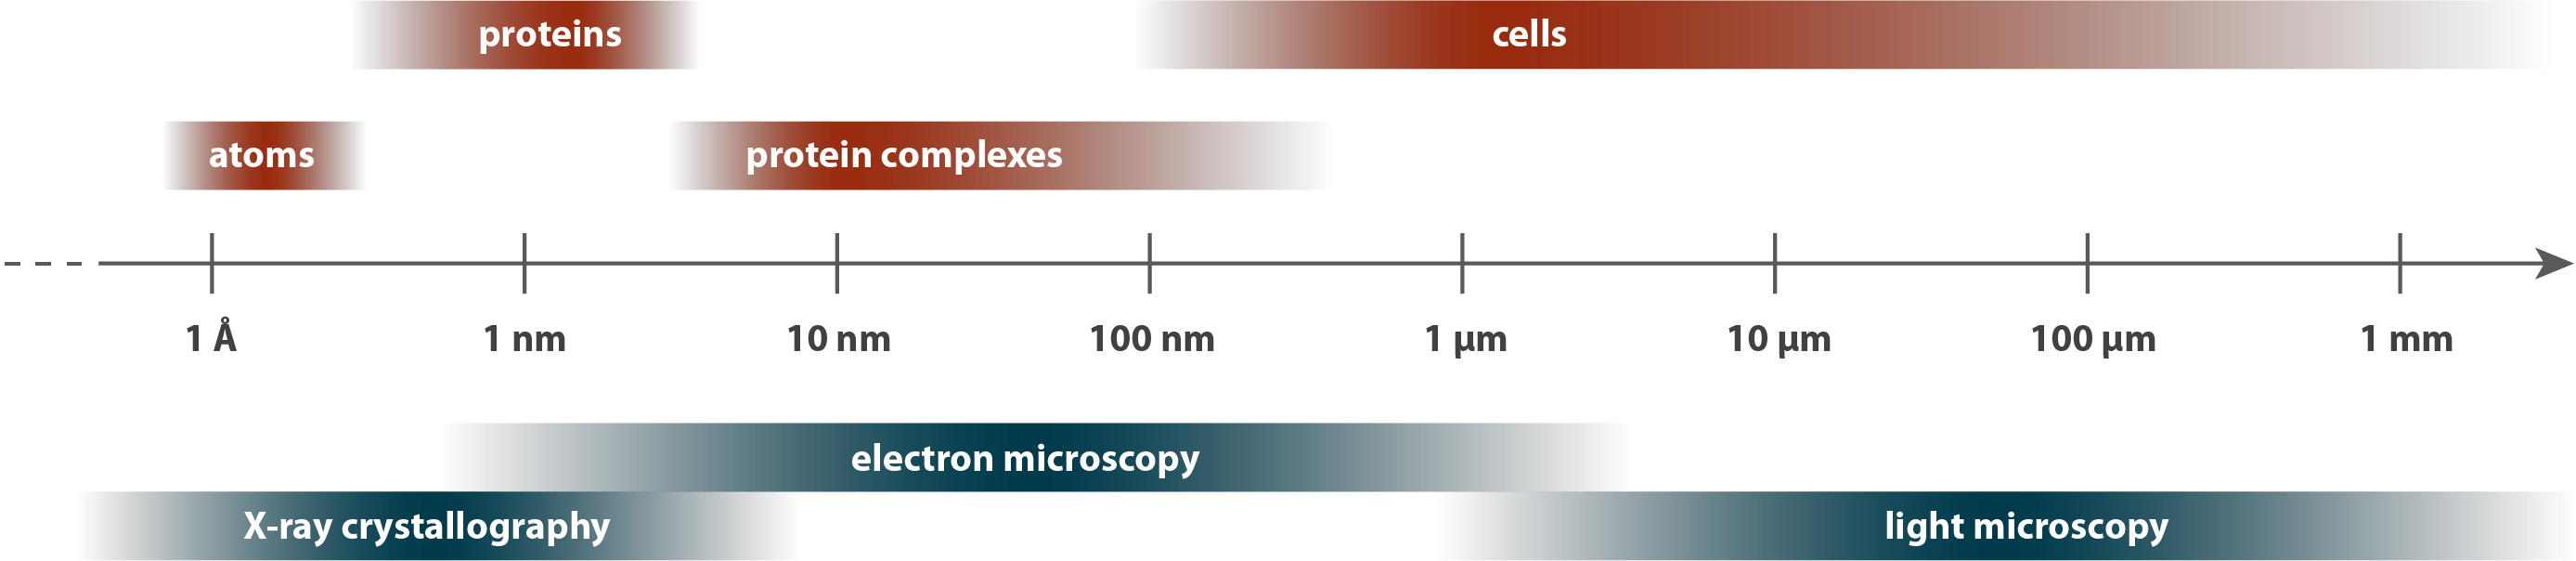
\includegraphics[width=38.54in]{img/schematics/1_1_1}

Cell biology occurs on a length scale that spans seven orders of magnitude. Different visualization techniques cover various sections of this span, as shown here with a few examples. Keep in mind that there are more techniques than these; we touch only on those you will see in the coming pages.

\hypertarget{fluorescence-light-microscopy}{%
\section{Fluorescence Light Microscopy}\label{fluorescence-light-microscopy}}

The addition of fluorescence to light microscopy allows us to look not just \emph{at} cells, but \emph{for} things inside them. Specific cellular components can be fluorescently labeled, with a stain or antibody that binds a particular molecule. Alternatively, a protein of interest can be genetically linked to a fluorescent protein such as Green Fluorescent Protein (GFP, isolated from a bioluminescent jellyfish off the Pacific coast in the 1970s and adapted as a revolutionary molecular biology tool in the 1990s). While tagging a protein can sometimes change its properties (e.g.~affecting its function or altering its localization), this technique often enables us to identify where in the cell a protein is found, and what it might be doing there.

As an example, this movie from Howard Berg's lab \citep{bergInternet} \citep{turner2000} shows \emph{Escherichia coli} cells stained by a fluorescent dye that binds to and highlights their flagella -- long, thin appendages that propel them through their environment. (We will discuss this and other ways cells move in Chapter 6.)



\hypertarget{htmlwidget-648949b5a0834a6111ef}{}

\label{fig:1-2}\protect\hyperlink{tree}{Escherichia coli} Collected by: \protect\hyperlink{howard_berg}{Howard Berg} Movie DOI: \href{https://doi.org/10.22002/D1.1464}{10.22002/D1.1464}

\hypertarget{scanning-electron-microscopy}{%
\section{Scanning Electron Microscopy}\label{scanning-electron-microscopy}}

While fluorescence allows us to highlight subcellular structures, we still cannot resolve much of their detail. This is because the resolution of microscopy is limited by the wavelength of the imaging beam. For light microscopy, the wavelength of the photons limits the resolution to a few hundred nanometers (more powerful for higher-energy blue light and less for lower-energy red). This resolving power is on the order of the width of many bacterial and archaeal cells. There are some technical ``super-resolution'' tricks to more finely pinpoint fluorescent molecules, but the overall subcellular details of bacteria and archaea are beyond the resolution of light microscopy.

One way to get around the resolution barrier is to use an imaging beam of higher-energy/shorter-wavelength particles. The discovery in the early 1900s that electrons have wave-like properties, and the subsequent realization that they can be focused by a ``lens'' consisting of a toroidal magnetic field, led to the development of electron microscopes in the 1930s.

There are two main types of electron microscopes \protect\hyperlink{Electron_microscopy_modes}{Schematic: Electron microscopy modes}. In a Scanning Electron Microscope (SEM), we detect electrons that are scattered backward from the sample, producing an image of the surface of the sample. The \emph{Shewanella oneidensis} cells you see here were imaged by SEM. Note the magnified details of the cells' shape and flagella compared to the light microscopy you just saw.



\hypertarget{htmlwidget-66dc37519f0f8974b112}{}

\label{fig:1-3}\protect\hyperlink{tree}{Shewanella oneidensis} Collected by: \protect\hyperlink{sahand_pirbadian}{Sahand Pirbadian} Movie DOI: \href{https://doi.org/10.22002/D1.1465}{10.22002/D1.1465}

\hypertarget{Electron_microscopy_modes}{%
\subsection*{Schematic: Electron microscopy modes}\label{Electron_microscopy_modes}}
\addcontentsline{toc}{subsection}{Schematic: Electron microscopy modes}

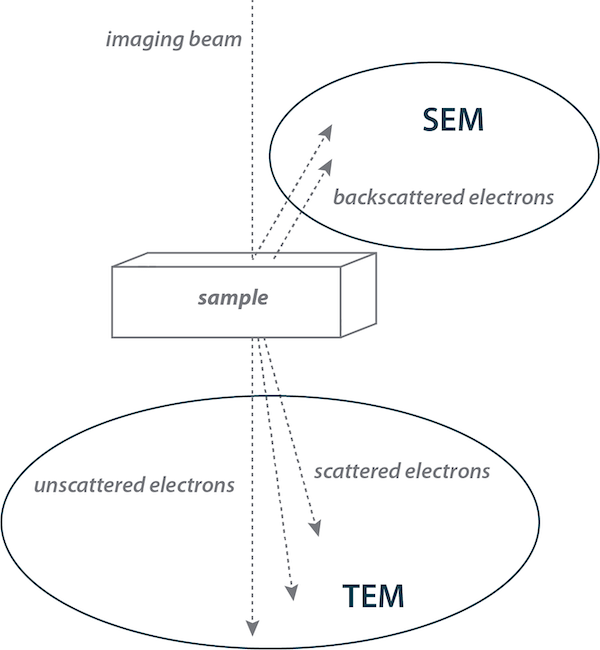
\includegraphics[width=8.33in]{img/schematics/1_3_1}

\hypertarget{transmission-electron-microscopy}{%
\section{Transmission Electron Microscopy}\label{transmission-electron-microscopy}}

In a Transmission Electron Microscope (TEM), we detect electrons that have interacted with atoms in the sample as they passed through it, producing a ``projection'' image of the 3D object onto a 2D plane, similar to a medical X-ray image. This shows details throughout the cell, not just on the surface.

Electron microscopy, whether SEM or TEM, relies on the interactions of electrons with biological material to create an image. These interactions, however, also present some problems. First, they damage the sample, so exposure has to be limited, which in turn limits the contrast of images, or how much signal we see relative to noise. Second, electrons interact not just with the sample, but also with anything else in their path, so imaging has to be conducted in a vacuum. This is problematic for biological material, which is mostly water that instantly boils away in a vacuum. To circumvent these problems, we can dehydrate samples to remove the water (changing the structure in the process) and coat them with metal to increase contrast. The \emph{Shewanella oneidensis} cells you saw on the last page were coated with platinum before imaging. In TEM, samples are often coated with a ``negative stain'' such as uranyl acetate; the electron-dense (dark in an image) metal pools around the sample, leaving the interior lighter and thereby creating a negative image. This \emph{S. oneidensis} cell was negative-stained this way before imaging. The resulting projection image again shows the shape of the cell and its flagellum, but not many internal details.

There are more elaborate (and structure-altering) sample preparation methods for TEM, involving fixing the sample by chemical crosslinking or freezing under high pressure, dehydrating it, embedding it in resin, staining it, and slicing it into thin sections. With these methods, electron microscopists were able to discover many details of eukaryotic cells such as their internal organelles. Bacteria and archaea are much smaller, though, and lack many robust prominent structures like organelles. As a result, until the twenty-first century, we thought bacteria and archaea were structurally unexciting, little more than water balloons filled with small molecules. How wrong we were.



\hypertarget{htmlwidget-687db3812cf2fb5f4153}{}

\label{fig:1-4}\protect\hyperlink{tree}{Shewanella oneidensis} Collected by: \protect\hyperlink{mohammed_kaplan}{Mohammed Kaplan} Movie DOI: \href{https://doi.org/10.22002/D1.1466}{10.22002/D1.1466}

\hypertarget{cryogenic-electron-microscopy}{%
\section{Cryogenic Electron Microscopy}\label{cryogenic-electron-microscopy}}

We are able to visualize the native structure of bacterial and archaeal cells thanks to a breakthrough in TEM sample preparation. Instead of getting rid of the water, why not just freeze it, since ice sublimates very slowly in a vacuum? Normally, the water would expand as it freezes into ice, damaging the cell in the process. But in the 1980s scientists discovered that freezing a sample quickly enough (done by rapidly plunging a small volume into a very efficient cryogen like liquid ethane) creates a very different kind of ice. The water molecules are immobilized so abruptly that they do not have a chance to find binding partners to form a crystal. The result, called ``vitreous'' ice for its glass-like properties, preserves cells in their native, fully-hydrated state. The frozen sample can then be inserted directly into the vacuum of the TEM without needing additional treatment or staining. This technique is called cryogenic electron microscopy, or cryoEM.

Here you see a projection image of a \emph{Caulobacter crescentus} cell imaged by cryoEM. Let's quickly go through how it was prepared. First a drop of culture was placed onto an EM grid. Instead of the glass slides used to support samples in a light microscope, EM sample supports are small circular grids of metal, \textasciitilde{}3 mm across, overlaid by thin mesh of carbon with 2 µm-wide holes. Excess liquid was then blotted away with paper, leaving a thin film of sample across the grid. The grid was then plunged into a cryogen, and the frozen sample was imaged in a special TEM that kept the sample in cryogenic conditions (at or below the temperature of liquid nitrogen) so that the vitreous ice didn't warm and transition to a more damaging (and opaque) crystalline state. In this image, you can see the edge of one of the holes in the carbon mesh of the grid; note the slightly increased clarity in the hole where there is nothing but culture media compared to the region with an additional layer of carbon. Whenever possible, we choose to image cells lying at least partially in holes. You will also notice many small dark circles -- these are gold beads that were added to the sample; you will see why on the next page.

With cryoEM, we can start to see the true structure of cells. Compared to the images you have already seen, note the added level of detail visible here, including the cell's multi-layered envelope, and the braided texture of its flagellum.



\hypertarget{htmlwidget-e89612e975fe4c8f075c}{}

\label{fig:1-5}\protect\hyperlink{tree}{Caulobacter crescentus} Collected by: \protect\hyperlink{steven_wang}{Steven Wang} Movie DOI: \href{https://doi.org/10.22002/D1.1467}{10.22002/D1.1467}

\hypertarget{electron-cryotomography}{%
\section{Electron Cryotomography}\label{electron-cryotomography}}

To truly understand a three-dimensional object, we need to be able to visualize it in three dimensions. To do that, we can use tomography (from the Greek for ``writing slices''). The process may be familiar from medical Computed Tomography, or CT, scans. Simply, the object is imaged from different angles (in a CT scan, the camera moves around the patient; in our case we keep the imaging path constant and simply rotate the small sample). This produces a ``tilt-series'' of projection images that can be digitally processed into a reconstruction of the 3D object--a tomogram. To do the reconstruction, we need to be able to precisely align the images, which is difficult because of the low contrast from cryoEM samples (unstained and sensitive to exposure). This is where the gold beads come in. As you saw on the previous page, they provide clear markers in the images to guide the alignment.

Here you see a tomogram of a \emph{Caulobacter crescentus} cell, which we view as a series of slices scanning (or ``writing'') from bottom to top. Note the further level of detail that this technique provides, separating the cell's structures into their three-dimensional locations. We can also rotate the tomogram and slice along a different axis to view structures from different angles, although not all angles are visible \protect\hyperlink{Missing_wedge}{Schematic: Missing wedge}.

Since the early 2000s, cryoET has transformed our understanding of microbial cells, revealing their structural richness and diversity, as you will see in the chapters that follow.



\hypertarget{htmlwidget-260b8bc69195686b6a00}{}

\label{fig:1-6}\protect\hyperlink{tree}{Caulobacter crescentus} Collected by: \protect\hyperlink{steven_wang}{Steven Wang} Movie DOI: \href{https://doi.org/10.22002/D1.1468}{10.22002/D1.1468}

\hypertarget{Missing_wedge}{%
\subsection*{Schematic: Missing wedge}\label{Missing_wedge}}
\addcontentsline{toc}{subsection}{Schematic: Missing wedge}

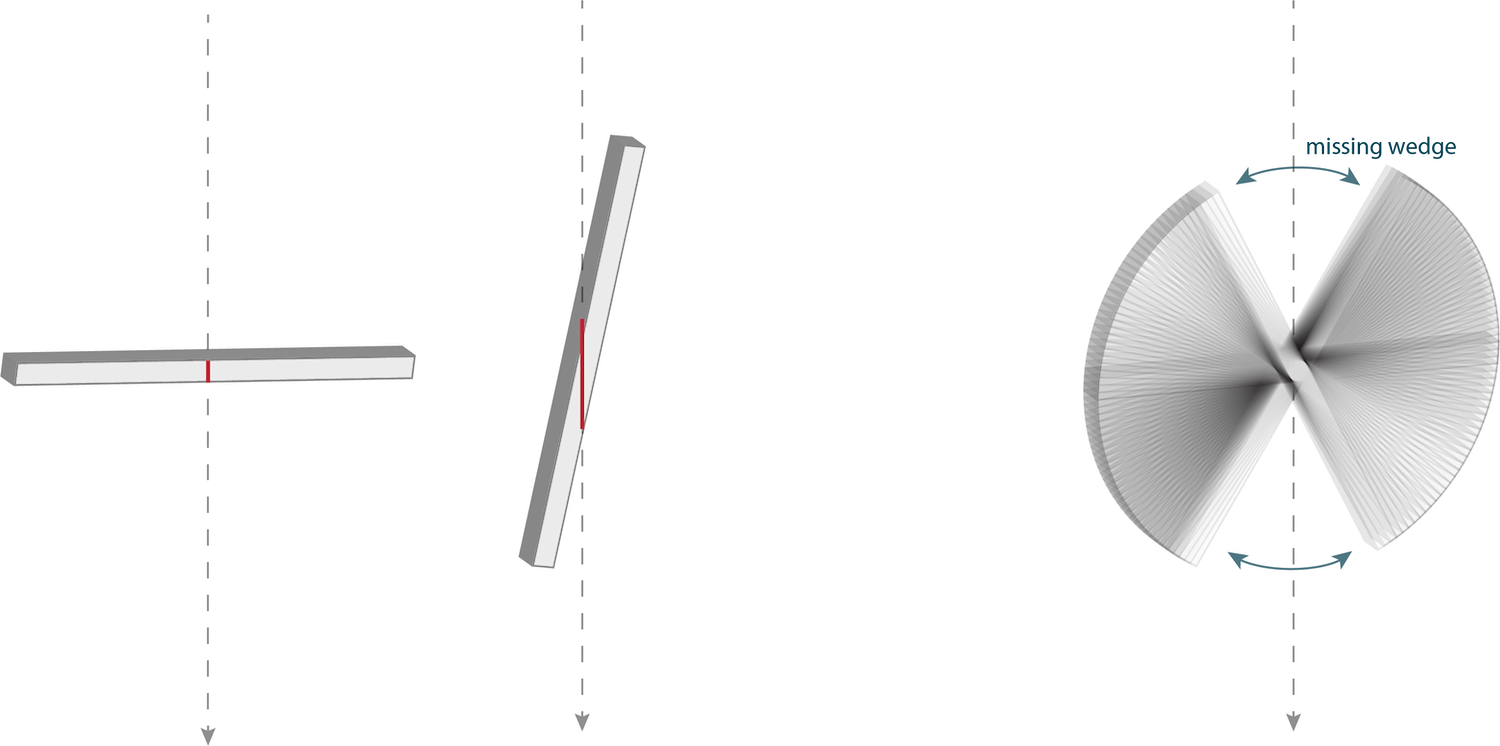
\includegraphics[width=20.83in]{img/schematics/1_6_1}

Think again about how a tilt-series is made: by taking images from different angles. If we could tilt the sample all the way to 90º, we would have information from every angle. But the sample gets effectively thicker as we tilt it, since the beam has to pass through more and more of the surrounding material. This effect usually becomes prohibitive beyond 60º, so a typical tilt-series spans only \textasciitilde{}2/3 of the possible angles, leaving a ``missing wedge'' of information corresponding to those high tilt angles, as you can see in this diagram. In practice, the missing wedge means that features at the top and bottom of the sample disappear. For instance, if we look at a cross-section of a cell, we cannot trace the membrane all the way around. For an example of this effect, check out the \emph{Caulobacter crescentus} cell in Chapter 5--FtsZ (cont'd.).

\hypertarget{sub-tomogram-averaging}{%
\section{Sub-Tomogram Averaging}\label{sub-tomogram-averaging}}

What if we want to zoom in further to examine a particular structure more closely? While in theory electron microscopy can resolve atoms, in practice the resolution is limited by the thickness of the sample. For relatively thick samples like the (small) bacterium on the last page, we can achieve \textasciitilde{}5 nm resolution, enough to see the shapes and arrangement of large macromolecular complexes. To boost our resolving power further, we can gather strength in numbers. By averaging multiple copies of a structure, either from the same tomogram, or from multiple cells in different tomograms, we can build up the signal relative to the noise. Here you see an example of this approach, called sub-tomogram averaging, applied to the motor that spins the flagellum. Hundreds of \emph{Campylobacter jejuni} cells were imaged by cryoET and their individual flagellar motors were extracted from the resulting tomograms and averaged to produce a higher-resolution view \citep{beeby2016}. Note how densities that vary between motors, indicating that they are not stably associated with the structure, get washed out, while densities that appear in the same place in each motor reinforce one another. This approach only works for structures, and parts of structures, that are fairly rigid, but it can be a powerful tool to study structures inside the cell. \href{https://www.ebi.ac.uk/pdbe/entry/emdb/emd-3150}{\emph{EMD-3150}}



\hypertarget{htmlwidget-4620334bc7f588c5ca37}{}

\label{fig:1-7}\protect\hyperlink{tree}{Campylobacter jejuni} Collected by: \protect\hyperlink{morgan_beeby}{Morgan Beeby} Movie DOI: \href{https://doi.org/10.22002/D1.1469}{10.22002/D1.1469}

\hypertarget{single-particle-reconstruction}{%
\section{Single Particle Reconstruction}\label{single-particle-reconstruction}}

If a structure can be purified out of the cell, we can zoom in even further. For a large, complex machine like the flagellar motor you just saw, particularly if it is embedded in the cell's membranes, the complete structure can only be studied in situ, inside the cell. But parts of it can be purified out of the cell and visualized by cryoEM single particle reconstruction. This technique is conceptually similar to sub-tomogram averaging, with many identical copies of a structure of interest averaging to produce a higher-resolution view. Instead of using tomography to see different angles, we take advantage of the fact that a random snapshot will capture individual copies in different orientations to provide all the views we need from just one or a few projection images. Usually tens of thousands of copies are averaged, often yielding resolutions of a few angstroms, sufficient to see the placement of each amino acid so that we can construct an atomic model of the structure like you see here. This structure, composed of 11 copies of a single protein, is the building block of the hook (the curved joint at the base of the flagellar filament) from \emph{Campylobacter jejuni} \citep{matsunami2016}. The next unit will stack into this one, and the next into that, and so on. Each complete hook contains about 100 copies of the protein monomer. \href{http://rcsb.org/structure/5JXL}{\emph{PDB: 5JXL}}

You will see many examples of high-resolution structures solved by this technique in the pages to come. It is mainly applied to large proteins and complexes, since most of the individual proteins in the cell are too small to be accurately aligned for reconstruction.



\hypertarget{htmlwidget-3e43d2f678cb04f2dd40}{}

\label{fig:1-8}\protect\hyperlink{tree}{Campylobacter jejuni} Collected by: \protect\hyperlink{matthias_wolffadel_samatey}{Matthias WolfFadel Samatey} Movie DOI: \href{https://doi.org/10.22002/D1.1470}{10.22002/D1.1470}

\hypertarget{x-ray-crystallography}{%
\section{X-Ray Crystallography}\label{x-ray-crystallography}}

For smaller protein complexes, we can use a different technique, based on photons produced by electron interactions: X-rays. This technique, too, relies on a kind of averaging of many particles, in this case identical molecules that have been purified from the cell and conditioned to form a 3D crystal. The wavelength of X-rays (\textasciitilde{}0.01 - 10 nm) is on the order of the distances between atoms in the crystal, which means that the atoms' electrons scatter the X-rays into a diffraction pattern that can be used to deduce the precise arrangement of each atom in the crystal. Beginning in the 1950s, X-ray crystallography has been enormously successful in revealing the structure of biological macromolecules like proteins and, famously, deoxyribonucleic acid (DNA) polymers \protect\hyperlink{Structural_biology_timeline}{Schematic: Structural biology timeline}.

Not every protein can be induced to form large, well-ordered crystals, but many can, and as of 2020, X-ray crystallography has been used to solve nearly 150,000 structures, including the one you see here, of a protein called FlgK from \emph{Campylobacter jejuni} \citep{bulieris2017}. 11 copies of this protein form a ring that caps the flagellar hook, acting as an adaptor between the hook joint and the long filament. \href{http://rcsb.org/structure/5XBJ}{\emph{PDB: 5XBJ}}



\hypertarget{htmlwidget-ecb9faa46ba3838af59a}{}

\label{fig:1-9}\protect\hyperlink{tree}{Campylobacter jejuni} Collected by: \protect\hyperlink{fadel_samatey}{Fadel Samatey} Movie DOI: \href{https://doi.org/10.22002/D1.1471}{10.22002/D1.1471}

\hypertarget{Structural_biology_timeline}{%
\subsection*{Schematic: Structural biology timeline}\label{Structural_biology_timeline}}
\addcontentsline{toc}{subsection}{Schematic: Structural biology timeline}

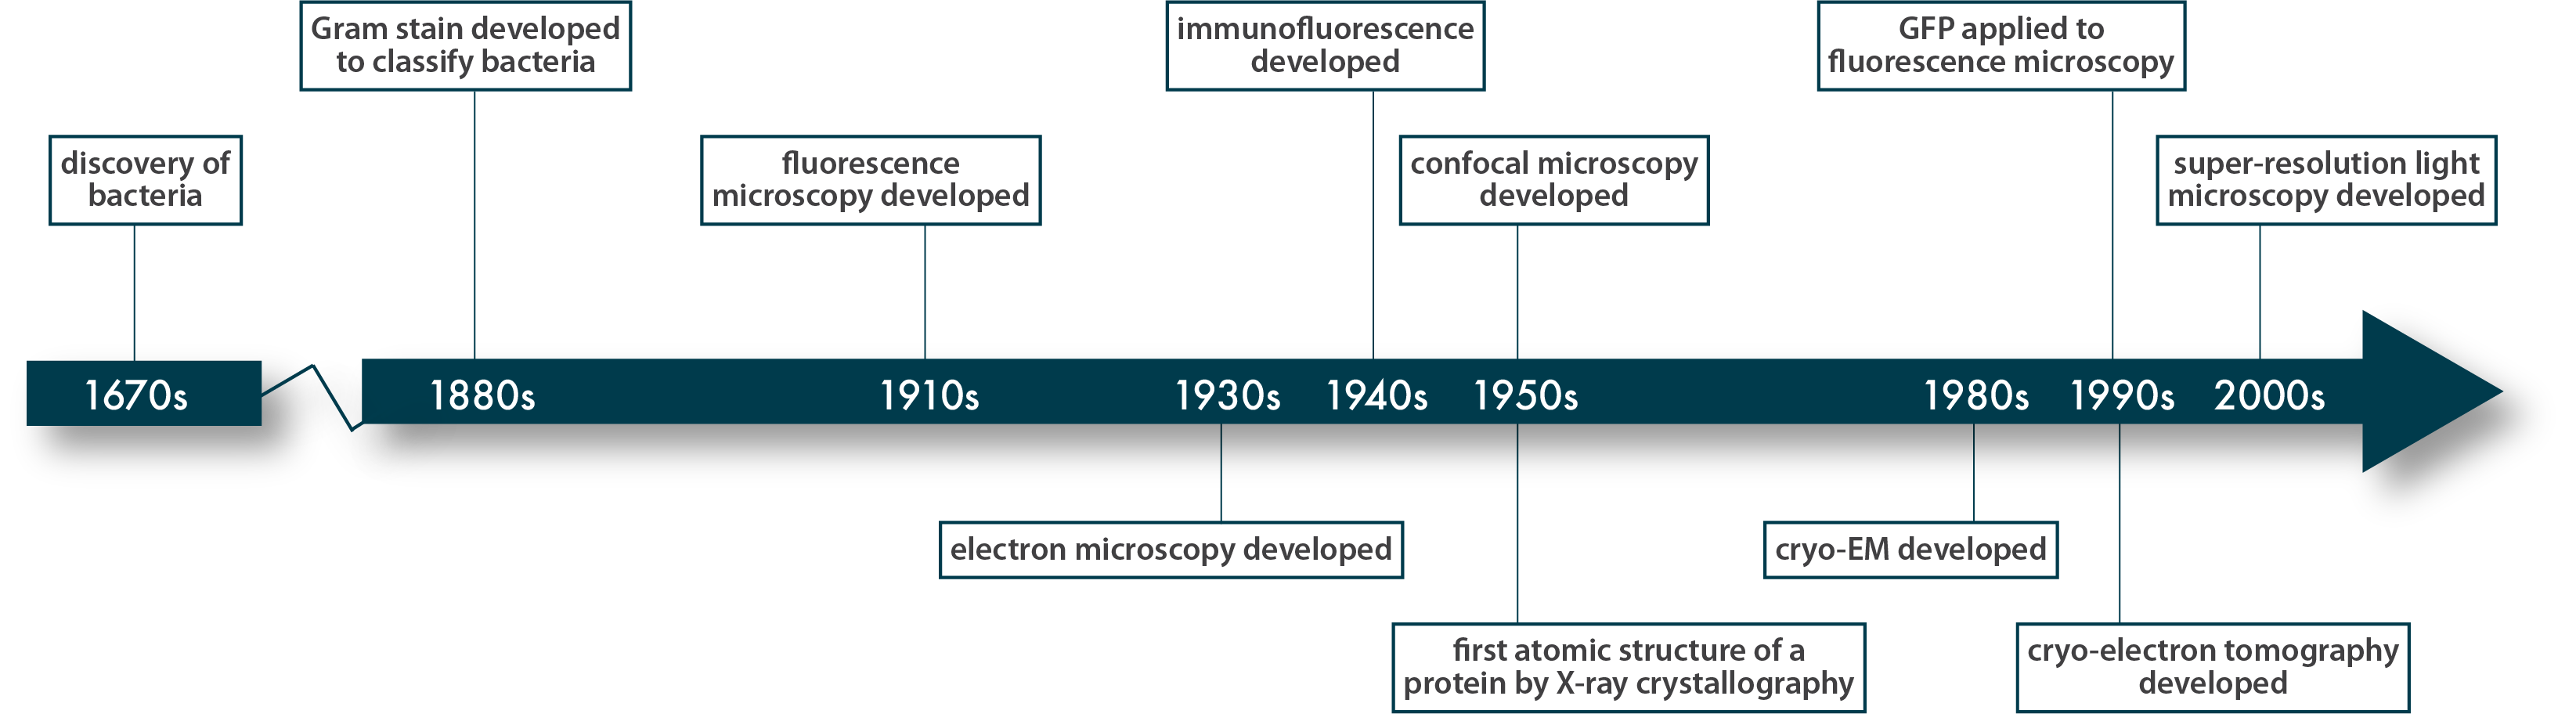
\includegraphics[width=45.69in]{img/schematics/1_9_1}

\hypertarget{putting-it-all-together}{%
\section{Putting It All Together}\label{putting-it-all-together}}

Science benefits from collaboration, and structural biology is no exception. This extends to our tools. To understand cells across their full length scale, we need to combine what we learn from different techniques. Consider this \emph{Bdellovibrio bacteriovorus} cell. We can visualize its overall structure by cryoET. We can identify particular substructures with the help of fluorescence light microscopy (this approach is called ``correlated light and electron microscopy''). We can get a higher-resolution view of an individual substructure by sub-tomogram averaging. We can then use genetics to identify the rough locations of individual components in that substructure by imaging mutants \protect\hyperlink{Difference_mapping}{More: Difference mapping}. Combining this analysis with positional clues from other biochemistry methods, we can place high-resolution structures of components solved by X-ray crystallography and single particle reconstruction into their correct context. In this way, we can begin to build up a full picture, from individual atoms to complete cells. We still have a long way to go, but someday we hope to be able to map the location and interactions of every protein in a bacterium or archaeon, creating a true atlas of the cell.



\hypertarget{htmlwidget-7f2fde3c8151634b64c9}{}

\label{fig:1-10}\protect\hyperlink{tree}{Bdellovibrio bacteriovorus} Collected by: \protect\hyperlink{yi-wei_chang}{Yi-Wei Chang} Movie DOI: \href{https://doi.org/10.22002/D1.1472}{10.22002/D1.1472}

\hypertarget{Difference_mapping}{%
\subsection*{More: Difference mapping}\label{Difference_mapping}}
\addcontentsline{toc}{subsection}{More: Difference mapping}

To identify the location of a component within a large macromolecular complex, difference mapping can be helpful. In this approach, the gene corresponding to that component is either knocked out or a tag is added, like GFP, that will make the protein larger. A subtomogram average of the complex is produced, and compared to a subtomogram average of the complex from wild-type (unmodified) cells. Often, a difference in the structure is visible, corresponding to the missing or altered component. Here you see an example of how this was used to locate a component of the flagellar motor, a protein called FliI, in \emph{Campylobacter jejuni} \citep{henderson2020}. \href{https://www.ebi.ac.uk/pdbe/entry/emdb/emd-5300}{\emph{EMD-5300}}; \href{https://www.ebi.ac.uk/pdbe/entry/emdb/emd-10457}{EMD-10457}



\hypertarget{htmlwidget-a63468cbe0eb1480f5db}{}

\label{fig:1-10a}\protect\hyperlink{tree}{Campylobacter jejuni} Collected by: \protect\hyperlink{morgan_beeby}{Morgan Beeby} Movie DOI: \href{https://doi.org/10.22002/D1.1473}{10.22002/D1.1473}

\hypertarget{further-reading}{%
\section{Further Reading}\label{further-reading}}

Chalfie et al. (1994). \emph{Green fluorescent protein as a marker for gene expression} \citep{chalfie1994}.

Jensen. \emph{Getting Started in Cryo-EM} Video Lectures \citep{jensenInternet}.

Oikonomou and Jensen (2017). \emph{Cellular electron cryotomography: toward structural biology in situ} \citep{oikonomou2017}.

Ruska (1987). \emph{Nobel Lecture: The development of the electron microscope and of electron microscopy} \citep{ruska1987}.

\hypertarget{envelope}{%
\chapter{Envelope}\label{envelope}}

\begin{quote}
``It is not a simple life to be a single cell, although I have no right to say so, having been a single cell so long ago myself that I have no memory at all of that stage of my life.''
- Lewis Thomas \citep{thomas1990}
\end{quote}

\hypertarget{membrane}{%
\section{Membrane}\label{membrane}}

The fundamental unit of life is the cell--a contained self-replicating assembly. For many species, including all bacteria and archaea, the organism consists of a single cell. And for nearly all species, no matter how many cells an organism eventually contains (probably around 10 trillion in your case), it started life as a single cell. The details vary, but every cell on Earth is the same at heart--a DNA-based replicating machine built from just four macromolecules: nucleic acids, proteins, lipids and carbohydrates.

Imagine for a moment that you are a structural engineer tasked with building one of these cells. Where would you start? How about the container? No matter what the first self-replicating molecules were (likely ribonucleic acid, or RNA), they were not a cell until they acquired a container. You would probably want a flexible container that allowed you to sort certain kinds of molecules from the environment. Evolution agrees. All cells are enclosed by a selectively permeable membrane, made of lipids and proteins \protect\hyperlink{Lipid_bilayer}{Schematic: Lipid bilayer}, that allows them to differentiate their contents from the environment. The selectivity of this membrane is a critical feature for the life of the cell \protect\hyperlink{ATP_synthase_and_energy_production}{Schematic: ATP synthase}.

Now your cell has a clearly delineated exterior and interior. The interior is called the cytoplasm (``cell mold,'' the membrane being the container that shapes the mold). Almost all archaea and many bacteria, like these \emph{Mycoplasma genitalium} cells, are monoderms (``single skin''). This means that their cytoplasm is enclosed by a single membrane. At this resolution, the membrane looks like a single dark line, but remember that it is really a bilayer, as you will be able to see in some later examples.



\hypertarget{htmlwidget-85e465c879532a216fb9}{}

\label{fig:2-1}\protect\hyperlink{tree}{Mycoplasma genitalium} Collected by: \protect\hyperlink{gregory_henderson}{Gregory Henderson} Movie DOI: \href{https://doi.org/10.22002/D1.1350}{10.22002/D1.1350}

\hypertarget{Lipid_bilayer}{%
\subsection*{Schematic: Lipid bilayer}\label{Lipid_bilayer}}
\addcontentsline{toc}{subsection}{Schematic: Lipid bilayer}

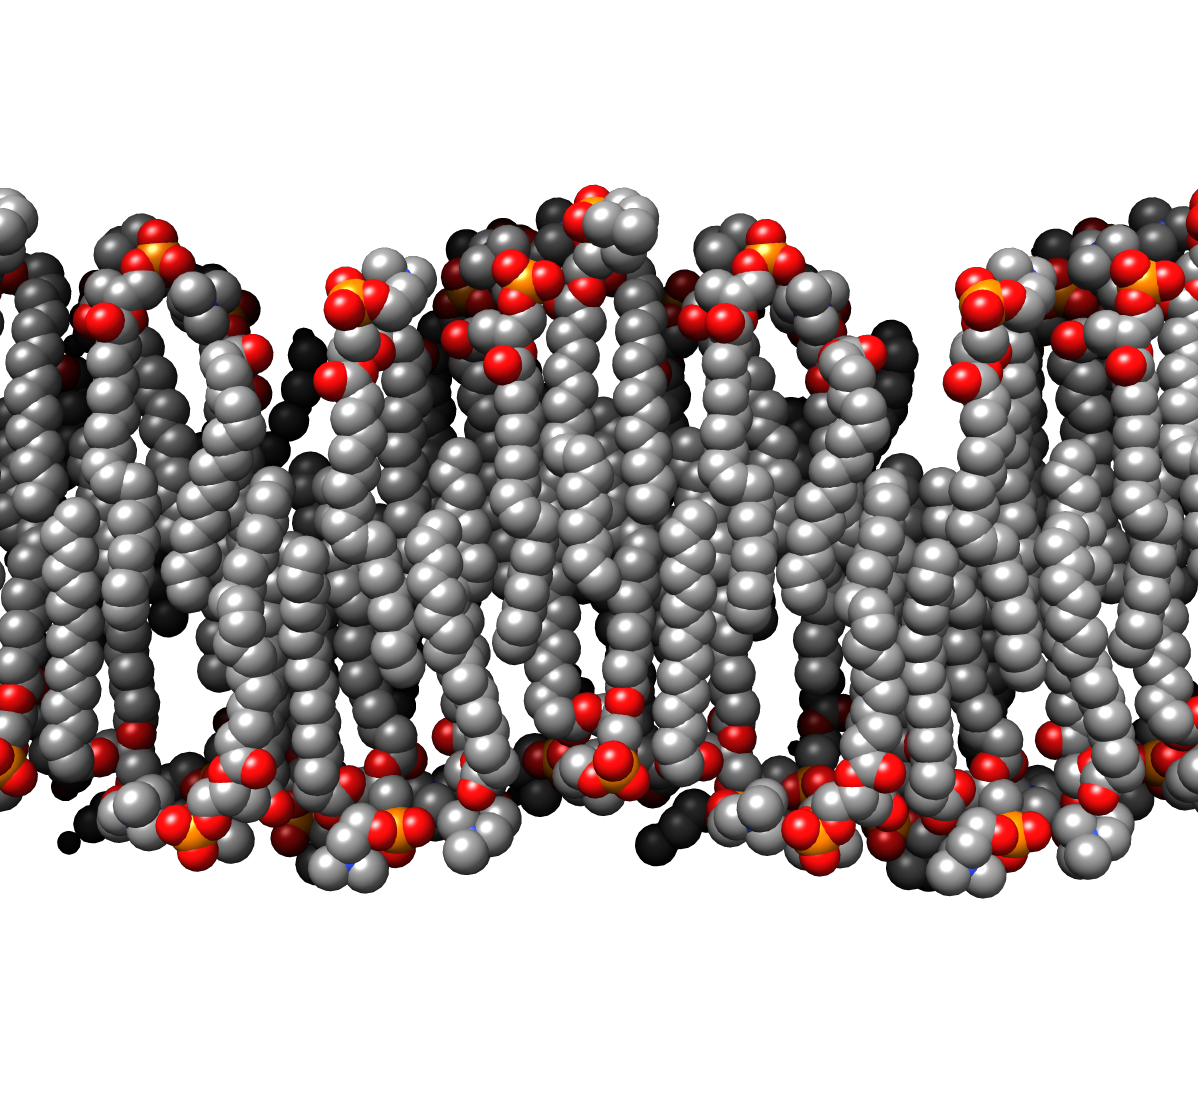
\includegraphics{img/schematics/2_1_1}

Lipids have a hydrophilic head (blue here) and hydrophobic tails (grey); in water they spontaneously pack side-by-side and tail-to-tail to shield their tails from unfavorable interactions with water. This results in closed double-layered bags--membranes. One key difference between archaea and bacteria (and with them, eukaryotes) is the kind of lipid in their membranes. Hybrid membranes containing both these lipid types can be made artificially, and it is possible that the last universal common ancestor of all cells on Earth contained both types, with specialization occurring later.

Membranes also contain many proteins. Some have hydrophobic regions that embed them into the lipid bilayer. Other proteins are fused, or tethered, to the lipids. In fact, cells' ``lipid'' membranes are made up of roughly equal parts lipids and proteins.

\hypertarget{ATP_synthase_and_energy_production}{%
\subsection*{Schematic: ATP synthase and energy production}\label{ATP_synthase_and_energy_production}}
\addcontentsline{toc}{subsection}{Schematic: ATP synthase and energy production}

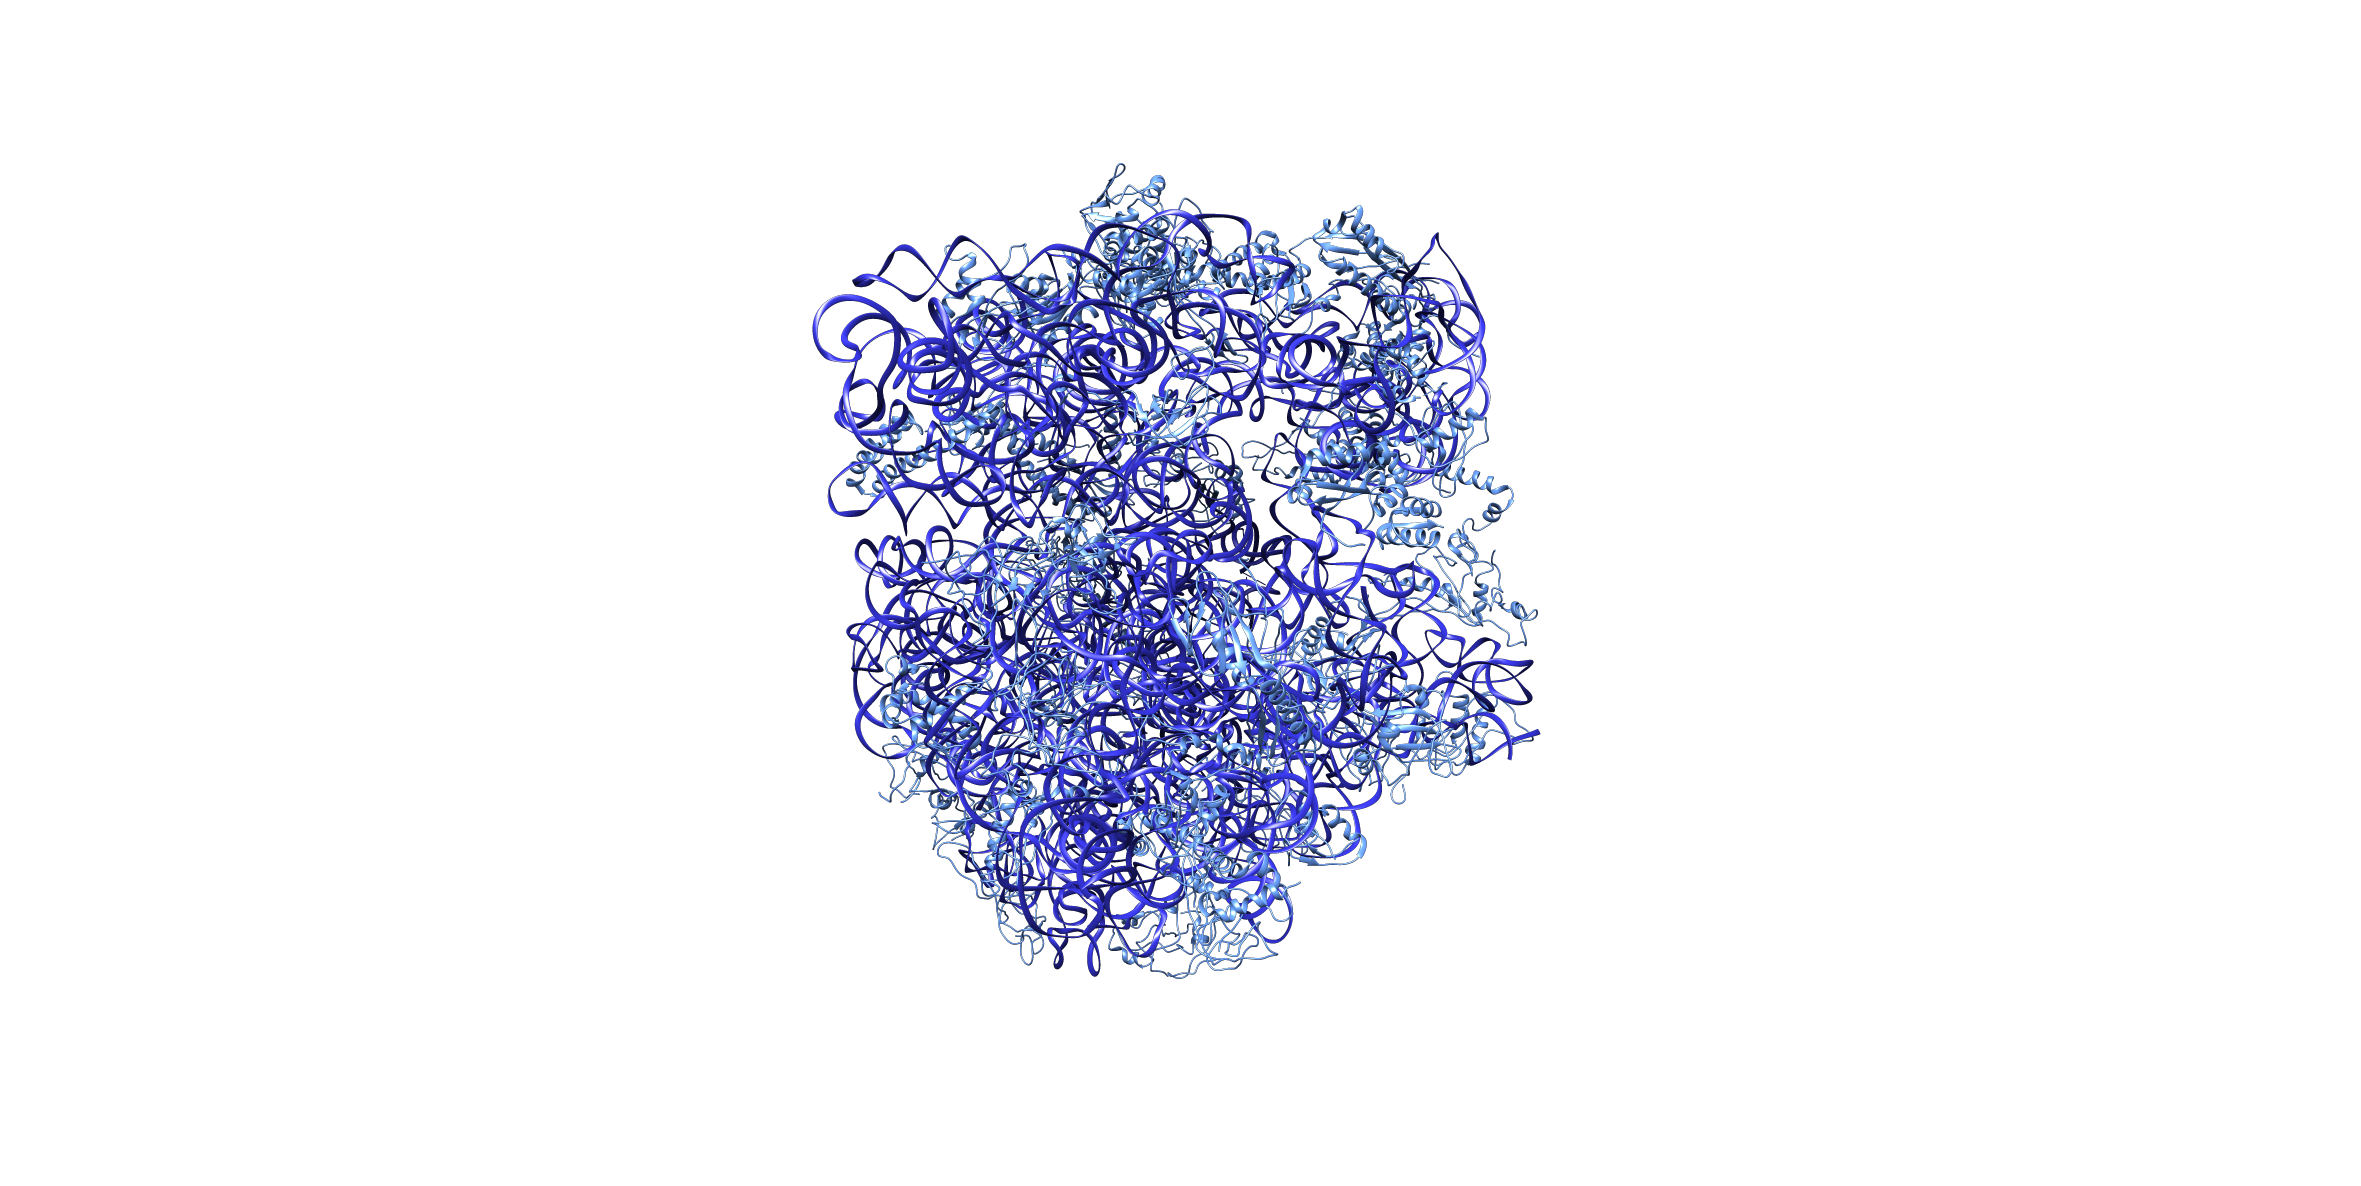
\includegraphics{img/schematics/2_1_2}

\href{http://rcsb.org/structure/5T4O}{\emph{PDB: 5T4O}}
The chemical properties of lipids make membranes impermeable to ions and large or hydrophilic molecules (but not to water). Cells take advantage of this property to establish an ion gradient across the membrane, using a chain of electron-carrying proteins in the membrane to pump protons out of the cell. Protein complexes in the membrane called ATP synthases (like this one from \emph{Escherichia coli} \citep{sobti2016}) use the resulting ion potential to generate energy. The machine provides a conduit for protons to flow down their potential, producing a ``proton-motive force'' that spins the machine's rotor, generating energy that is chemically stored in ATP, the energetic currency of the cell. For this reason, we say that the membrane is ``energized.'' Holes in the membrane allow the ion gradient to equilibrate, destroying the cell's means of generating energy, and thus its life.

\hypertarget{cell-wall}{%
\section{Cell Wall}\label{cell-wall}}

Being able to selectively move things into your cell enables it to do some powerful things. It also poses a structural problem. Remember that water can pass freely through the membrane, which means that increasing the solute concentration inside relative to the environment outside will cause water to rush in as well, introducing a pressure (known as turgor pressure) on the membrane. Lipid bilayers, unfortunately, are unable to withstand much pressure. If your cell lives exclusively in a constant, and fairly high-osmolarity, environment (like our bodies, in the case of the pathogenic \emph{Mycoplasma genitalium} you just saw), it can balance internal and external osmolarity to minimize turgor pressure on its membrane. But most cells experience more variable, and dilute, environments. How could you keep your cell from bursting in such conditions?

You might want to add some rigid scaffolding outside the membrane to buttress it against turgor pressure. Nearly all bacteria do this with a material called peptidoglycan: long stiff polymers of glycan sugars crosslinked by short peptides into a chain-mail-like mesh. The full scaffold of this material surrounding the cell is called its sacculus, or cell wall. In monoderm bacteria like this \emph{Listeria monocytogenes}, the cell wall is significantly thicker than the membrane. It comprises several layers of peptidoglycan, which are indistinguishable at this resolution, so the cell wall appears as a uniformly textured layer \protect\hyperlink{Peptidoglycan_architecture}{More: Peptidoglycan architecture}. It remains a mystery how large molecules can pass through this dense layer on their way to and from the cell.

While most bacteria build their walls from peptidoglycan, some use slightly different materials \protect\hyperlink{Methanobacterium_formicicum}{More: Methanobacterium formicicum}. Some archaea also have cell walls, also made of a molecule similar to peptidoglycan, but chemically distinct. Most archaea, though, rely on a different structure for support, which you will see in a few pages.

A wall can be a boon to your cell, but it can also prove a liability in certain conditions. For instance, many antibiotics target the cell wall. Some bacteria have developed the ability to jettison their walls in such conditions, taking on a so-called ``L-form'' (named for the Lister Institute where it was discovered). L-form bacteria give us a fascinating window into how early cells--prior to the evolution of the cell wall--might have looked and behaved.



\hypertarget{htmlwidget-e3f254b1bd354f7577b8}{}

\label{fig:2-2}\protect\hyperlink{tree}{Listeria monocytogenes} Collected by: \protect\hyperlink{ariane_briegel}{Ariane Briegel} Movie DOI: \href{https://doi.org/10.22002/D1.1351}{10.22002/D1.1351}

\hypertarget{Peptidoglycan_architecture}{%
\subsection*{More: Peptidoglycan architecture}\label{Peptidoglycan_architecture}}
\addcontentsline{toc}{subsection}{More: Peptidoglycan architecture}

The sacculus is so robust that it persists even after cells are lysed and their other components digested. This sacculus isolated from a \emph{Bacillus subtilis} cell has retained its shape, simply flattening with the release of contents and pressure from inside. The long glycan strands are oriented in hoops running parallel to the short axis of the cylindrical cell and the short peptide crosslinks are more or less aligned with the long axis.



\hypertarget{htmlwidget-053667247b8eb8339b7d}{}

\label{fig:2-2a}\protect\hyperlink{tree}{Bacillus subtilis} Collected by: \protect\hyperlink{morgan_beeby}{Morgan Beeby} Movie DOI: \href{https://doi.org/10.22002/D1.1360}{10.22002/D1.1360}

\hypertarget{Methanobacterium_formicicum}{%
\subsection*{More: Methanobacterium formicicum}\label{Methanobacterium_formicicum}}
\addcontentsline{toc}{subsection}{More: Methanobacterium formicicum}

These methane-producing bacteria, found in the rumen of animals like cows, build their walls with a polymer that has a slightly different chemical composition than peptidoglycan, but which forms a similar structure, as you can see.



\hypertarget{htmlwidget-1f73f0d3ffe616f601c5}{}

\label{fig:2-2b}\protect\hyperlink{tree}{Methanobacterium formicicum} Collected by: \protect\hyperlink{elitza_tocheva}{Elitza Tocheva} Movie DOI: \href{https://doi.org/10.22002/D1.1361}{10.22002/D1.1361}

\hypertarget{outer-membrane}{%
\section{Outer Membrane}\label{outer-membrane}}

Why stop at one membrane? Eukaryotic cells use internal membranes to form specialized compartments like the nucleus and mitochondria. While bacteria lack such organelles, many create an additional compartment \emph{outside} the cell with a second, outer, membrane. Such bacteria, like the \emph{Cupriavidus necator} cell you see here, are called diderms (``double skin''). The extra compartment between their membranes is known as the periplasm (``mold between''). This antechamber contains a unique subset of proteins, many of which function in escorting things into and out of the main cell.

Compared to the inner membrane, the outer membrane has some unique properties. It is more permeable and not proton-tight (so it cannot be used to generate ATP). It is often asymmetric, with a different composition of lipids and proteins in each of the two leaflets. A few species of bacteria, particularly pathogens, have labile outer membranes (for an example, check out the \emph{Helicobacter pylori} in Chapter 8--Genome Protection). Most, however, firmly anchor their outer membrane to the cell wall \protect\hyperlink{Brauns_lipoprotein}{Schematic: Braun's lipoprotein}. Rather than containing many layers of peptidoglycan like in the \emph{Listeria monocytogenes} cell you just saw, the cell wall of diderms is usually composed of a single layer of peptidoglycan mesh \protect\hyperlink{Diderm_sacculus_architecture}{More: Diderm sacculus architecture}, which is visible here as a thin line in the periplasm. This minimal sacculus presents a considerable challenge for growth: how can you remodel a single-layered wall that is under pressure? The answer, as we are beginning to figure out, is very carefully \protect\hyperlink{Sacculus_remodeling}{Schematic: Sacculus remodeling}.

The difference in thickness of monoderm and diderm cell walls enables a well-known classification system: the Gram stain, which binds peptidoglycan. Gram-positive bacteria, typically monoderm, contain much more peptidoglycan than Gram-negative bacteria, which are typically diderm.



\hypertarget{htmlwidget-2e9482130b1f9bc1c506}{}

\label{fig:2-3}\protect\hyperlink{tree}{Hydrogenovibrio crunogenus} Collected by: \protect\hyperlink{cristina_iancu}{Cristina Iancu} Movie DOI: \href{https://doi.org/10.22002/D1.1352}{10.22002/D1.1352}

\hypertarget{Brauns_lipoprotein}{%
\subsection*{Schematic: Braun's lipoprotein}\label{Brauns_lipoprotein}}
\addcontentsline{toc}{subsection}{Schematic: Braun's lipoprotein}

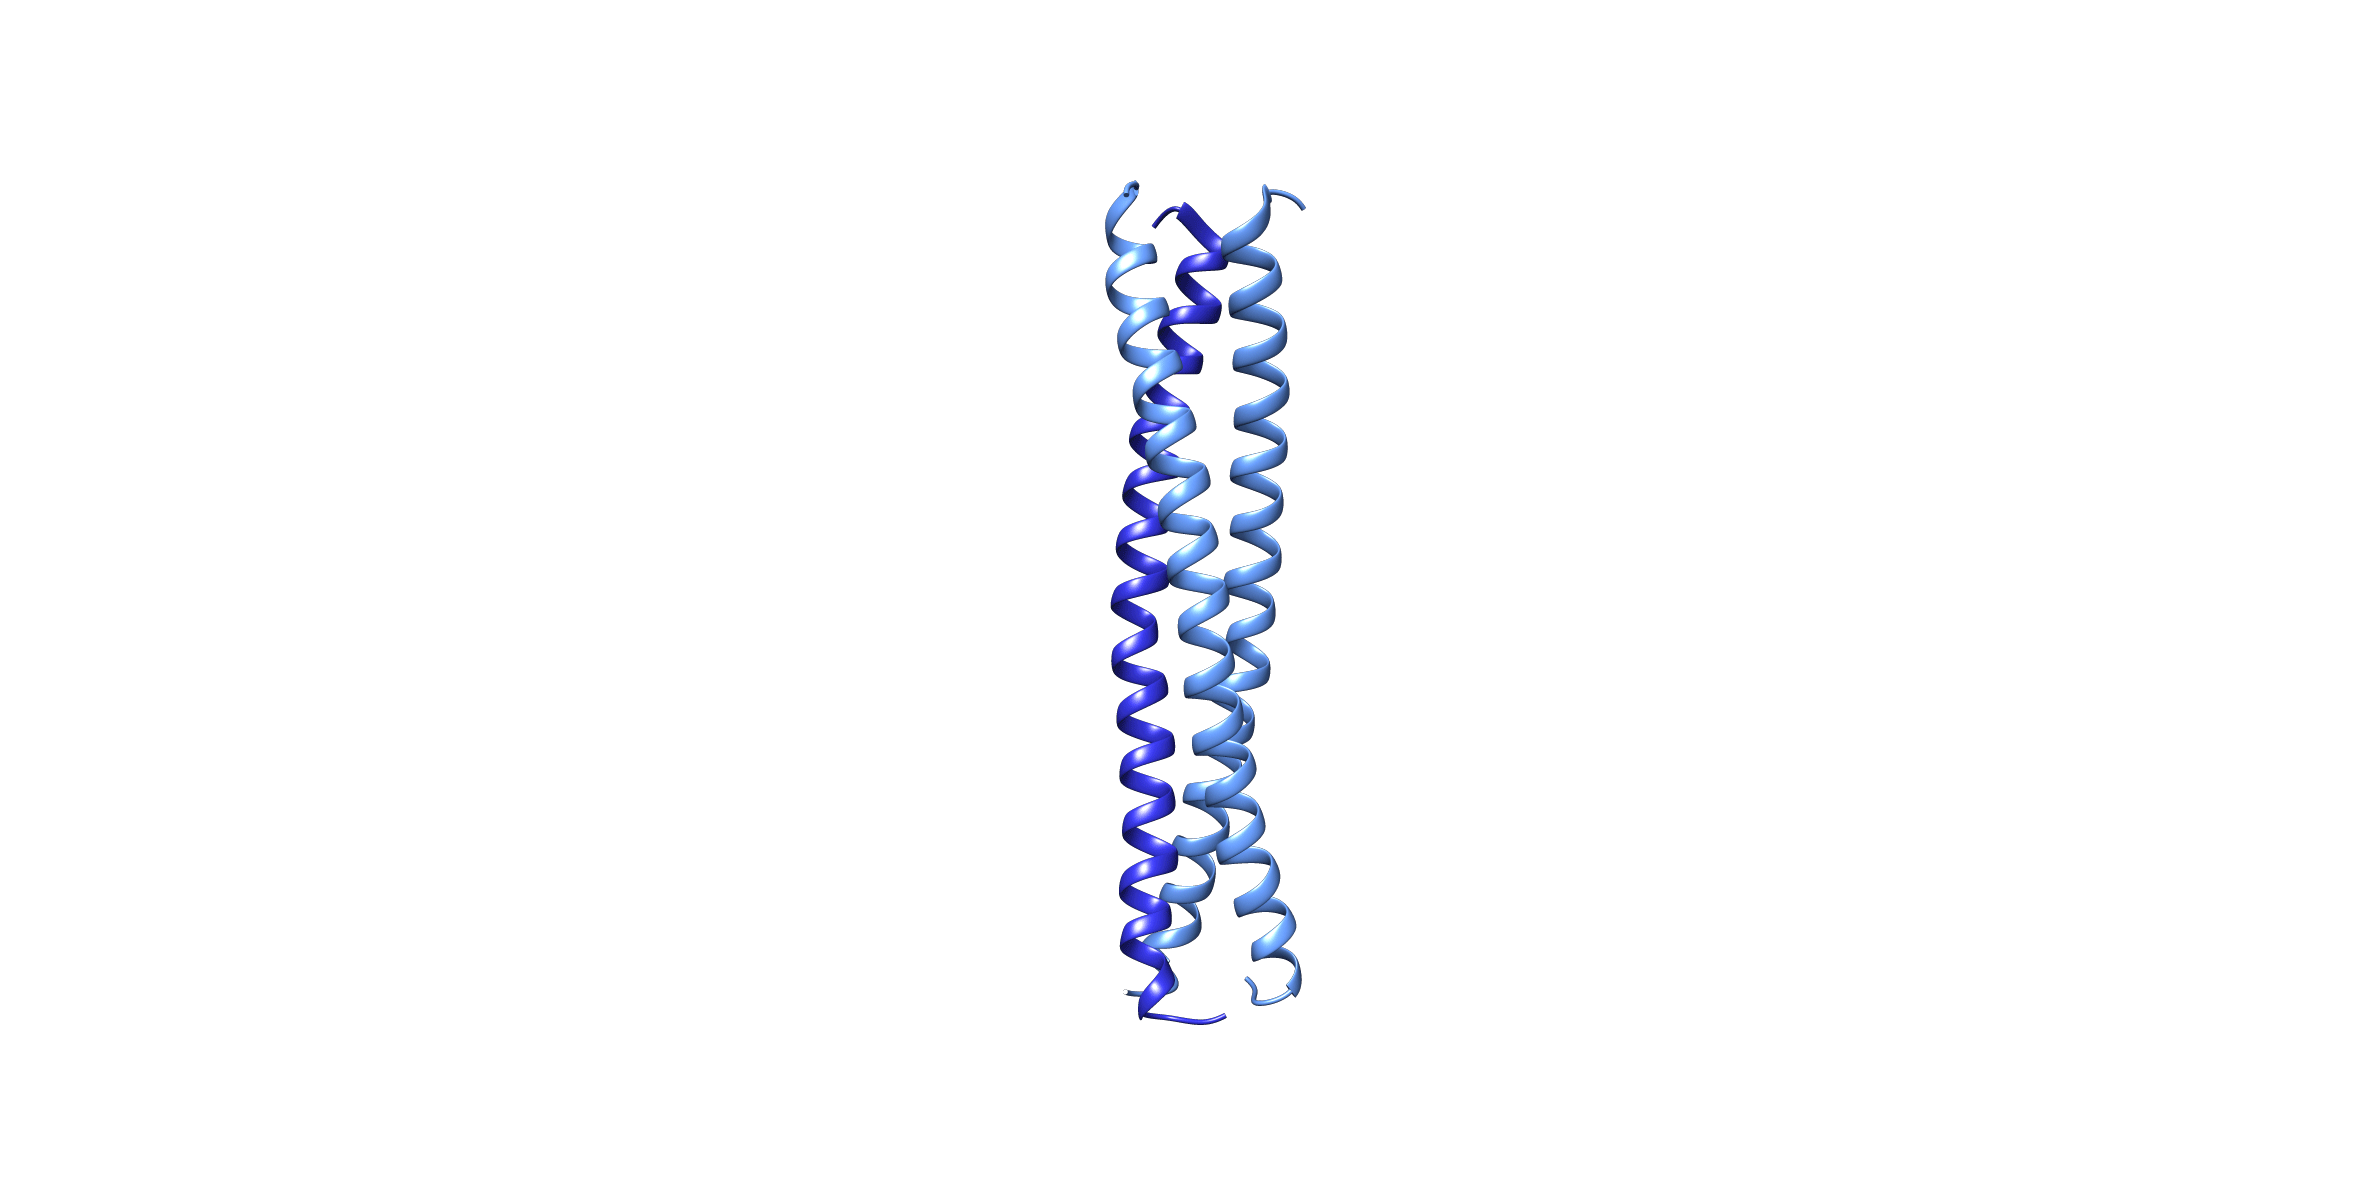
\includegraphics{img/schematics/2_3_1}

\href{http://rcsb.org/structure/1EQ7}{\emph{PDB: 1EQ7}}
Lipoproteins are hybrid molecules, formed by covalently-linked lipid and protein pieces. The lipid allows them to embed into a membrane, tethering the attached protein to function nearby. Braun's lipoprotein, or Lpp \citep{shu2000}, is one of the most abundant molecules in the outer membrane of cells like \emph{Escherichia coli}. The top of the trimeric protein ``coiled-coil'' shown here contains the lipid tether. The bottom binds the peptidoglycan cell wall, creating a link between the outer membrane and the cell wall (adding up, for a typical \emph{E. coli} cell, to about 100,000 links). These links set the distance between the two layers.

\hypertarget{Diderm_sacculus_architecture}{%
\subsection*{More: Diderm sacculus architecture}\label{Diderm_sacculus_architecture}}
\addcontentsline{toc}{subsection}{More: Diderm sacculus architecture}

Compare this diderm sacculus purified from \emph{Escherichia coli} to the monoderm sacculus on the last page. Since this one is thinner, we can make out more details, like the glycan strands running around the circumference of the cell. The main difference between the two types of sacculi seems to be whether they have largely a single layer of peptidoglycan (diderm) or many layers (monoderm). So even though the two types of wall look different, their architecture is fundamentally the same. In some circumstances, as you will see in Chapter 8, cells can even switch between the two forms.



\hypertarget{htmlwidget-8307057cff1c493c65be}{}

\label{fig:2-3a}\protect\hyperlink{tree}{Escherichia coli} Collected by: \protect\hyperlink{lu_gan}{Lu Gan} Movie DOI: \href{https://doi.org/10.22002/D1.1362}{10.22002/D1.1362}

\hypertarget{Sacculus_remodeling}{%
\subsection*{Schematic: Sacculus remodeling}\label{Sacculus_remodeling}}
\addcontentsline{toc}{subsection}{Schematic: Sacculus remodeling}

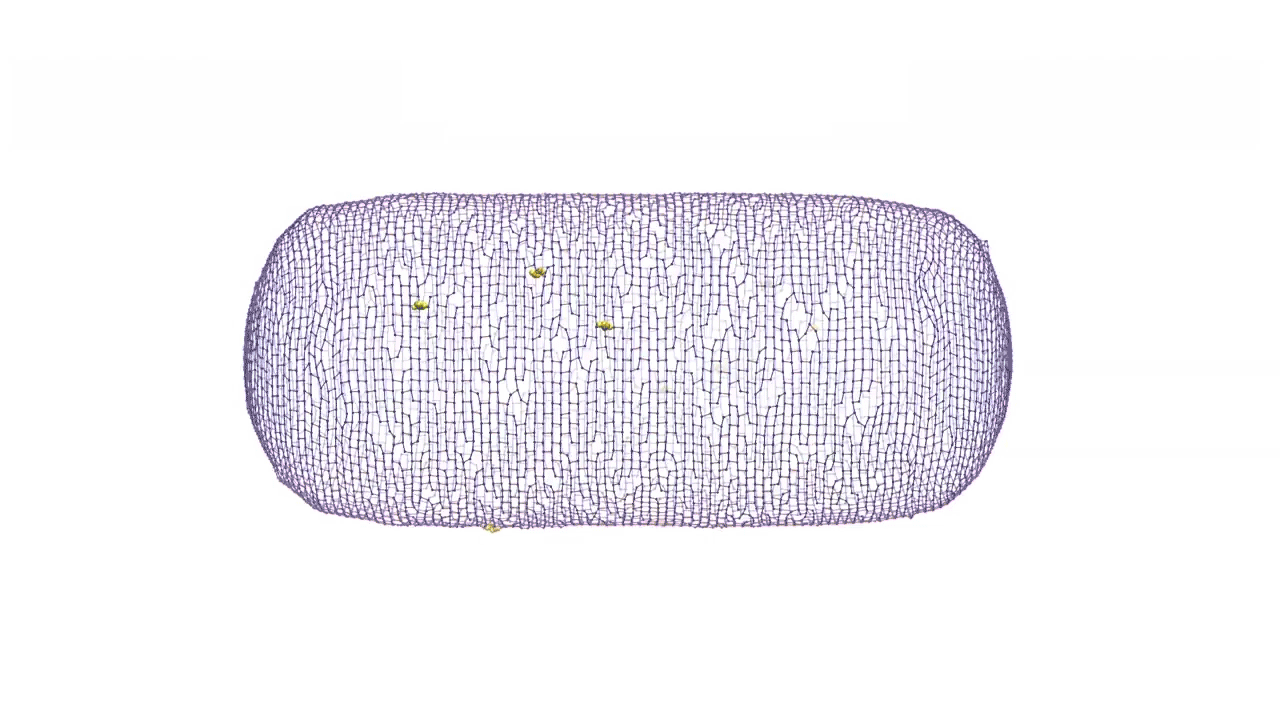
\includegraphics{img/schematics/2_3_2}

Encasing your cell in a rigid scaffold presents a problem: how can it grow? It is easy to make membranes larger simply by adding more lipids. But to add more peptidoglycan strands, they must be linked into the existing network, which means breaking existing links to accommodate them. To do this, cells use three tools: an enzyme that links glycan sugars into strands, an enzyme that links glycan strands together with peptide bonds, and an enzyme that cuts these peptide links to allow new strands to be incorporated. Remember, though, that your cell, with its solute-rich interior, has a turgor pressure pushing outward with a force of perhaps 3 atmospheres, equivalent to what we would feel at a depth of 20 meters in the ocean. This is more than enough pressure to lyse an exposed membrane, so the tools must be wielded with care or the cell would burst. We are still figuring out how this works, with help from computer simulations like this one. Here you see a model of an \emph{Escherichia coli} sacculus being enlarged using the three enzyme tools we just described (the colored balls). This simulation was run to test whether just having the tools function in a complex rather than separately might provide enough coordination for smooth, safe growth \citep{nguyen2015}. (The answer was yes.)

\hypertarget{vesicles}{%
\section{Vesicles}\label{vesicles}}

What else can your cell do with an extra membrane? Since membranes make such excellent containers for molecules, why not get into the shipping business? In the coming chapters (especially Chapter 9), you will see some of the ways that cells interact with each other and their environment. For diderm bacteria, many of these interactions are made possible by outer membrane vesicles (``little bladders'')--self-contained pockets budded off the membrane. The vesicles may carry cargo of antibiotics to inhibit competitors' growth, or toxins to lyse neighboring cells. Or enzymes to digest those lysed remains into nutrients that your cell can easily take up as food. Alternatively, they may carry emergency kits, first aid and survival factors for other members of a community biofilm. The appearance of these vesicles can vary as much as their contents \protect\hyperlink{Pearled_vesicles}{More: Pearled vesicles}; \protect\hyperlink{Tubular_vesicles}{More: Tubular vesicles}. They are usually spherical, though, of a fairly consistent size, and often come off the cell at one or a few sites, forming chains, as you can see in this \emph{Myxococcus xanthus} cell.

Not all diderms produce outer membrane vesicles, and even for those that do, we still do not know exactly how they do it. Maybe it happens spontaneously due to the physics of lipids and proteins in a certain configuration. Or maybe there is a dedicated protein machine in the membrane, blowing bubbles. Vesicles can also bud from the cytoplasmic or (for monoderms) inner membrane into the cytoplasm or periplasm \protect\hyperlink{Cytoplasmic_vesicles}{More: Cytoplasmic vesicles}. This seems to be a less regulated process than outer membrane vesicle formation, and we see it in many species when they are stressed by low nutrients or high cell density, suggesting that it is a general phenomenon. Cells shrink in harsh conditions (more on that in Chapter 8), so cytoplasmic or periplasmic vesicles may simply offer a place to put the extra membrane until the time comes to grow again. Just as with outer membrane vesicles, the appearance of cytoplasmic vesicles varies widely \protect\hyperlink{Cytoplasmic_vesicle_variety}{More: Cytoplasmic vesicle variety}. Archaea also produce membrane vesicles, both extracellular and cytoplasmic \protect\hyperlink{Archaeal_vesicles}{More: Archaeal vesicles}. They have been studied less than their bacterial counterparts, but likely serve similar roles in metabolism and community interactions.



\hypertarget{htmlwidget-e40733d741a83a2afcfe}{}

\label{fig:2-4}\protect\hyperlink{tree}{Myxococcus xanthus} Collected by: \protect\hyperlink{yi-wei_chang}{Yi-Wei Chang} Movie DOI: \href{https://doi.org/10.22002/D1.1474}{10.22002/D1.1474}

\hypertarget{Pearled_vesicles}{%
\subsection*{More: Pearled vesicles}\label{Pearled_vesicles}}
\addcontentsline{toc}{subsection}{More: Pearled vesicles}

Different species can produce outer membrane vesicles that look very different. Even vesicles from the same species can look very different. Sometimes they come off the cell as a chain of spheres; sometimes the spheres remain connected, like a string of pearls, as in this \emph{Borrelia burgdorferi} cell. Sometimes vesicles form long tubes instead \protect\hyperlink{Tubular_vesicles}{More: Tubular vesicles}. Sometimes the same chain can be tubular in one section (usually at the base, connected to the cell), and a string of spheres in another.



\hypertarget{htmlwidget-2ca696f089ddbcbb42d1}{}

\label{fig:2-4a}\protect\hyperlink{tree}{Borrelia burgdorferi 2} Collected by: \protect\hyperlink{ariane_briegel}{Ariane Briegel} Movie DOI: \href{https://doi.org/10.22002/D1.1363}{10.22002/D1.1363}

\hypertarget{Tubular_vesicles}{%
\subsection*{More: Tubular vesicles}\label{Tubular_vesicles}}
\addcontentsline{toc}{subsection}{More: Tubular vesicles}

Here, again from a \emph{Borrelia burgdorferi} cell, you can see extended, tubular outer membrane vesicles.



\hypertarget{htmlwidget-7a3c911f7c4df387c2d0}{}

\label{fig:2-4b}\protect\hyperlink{tree}{Borrelia burgdorferi} Collected by: \protect\hyperlink{ariane_briegel}{Ariane Briegel} Movie DOI: \href{https://doi.org/10.22002/D1.1353}{10.22002/D1.1353}

\hypertarget{Cytoplasmic_vesicles}{%
\subsection*{More: Cytoplasmic vesicles}\label{Cytoplasmic_vesicles}}
\addcontentsline{toc}{subsection}{More: Cytoplasmic vesicles}

Not all vesicles come from the outer membrane. The cytoplasmic or inner membrane can also form vesicles that are released into the cytoplasm, as in this \emph{Myxococcus xanthus} cell, or into the periplasm.



\hypertarget{htmlwidget-bce732e5e1aaa7d18081}{}

\label{fig:2-4c}\protect\hyperlink{tree}{Myxococcus xanthus} Collected by: \protect\hyperlink{matthew_swulius}{Matthew Swulius} Movie DOI: \href{https://doi.org/10.22002/D1.1364}{10.22002/D1.1364}

\hypertarget{Cytoplasmic_vesicle_variety}{%
\subsection*{More: Cytoplasmic vesicle variety}\label{Cytoplasmic_vesicle_variety}}
\addcontentsline{toc}{subsection}{More: Cytoplasmic vesicle variety}

Cytoplasmic vesicles exhibit a variety of sizes and shapes. Some are nested, with vesicles inside vesicles. In this \emph{Prosthecobacter debontii} cell, you can see two other morphologies. One resembles a flattened horseshoe. Another is a more typical spherical shape, but is decorated with what look like protein complexes.

This cell also has unusual structures on its surface that have yet to be identified.



\hypertarget{htmlwidget-676407a9a13e94f947c7}{}

\label{fig:2-4d}\protect\hyperlink{tree}{Prosthecobacter debontii} Collected by: \protect\hyperlink{martin_pilhofer}{Martin Pilhofer} Movie DOI: \href{https://doi.org/10.22002/D1.1365}{10.22002/D1.1365}

\hypertarget{Archaeal_vesicles}{%
\subsection*{More: Archaeal vesicles}\label{Archaeal_vesicles}}
\addcontentsline{toc}{subsection}{More: Archaeal vesicles}

Just like bacteria, archaea also produce both internal and external vesicles, as you can see in this \emph{Halomicrobium mukohataei} cell.



\hypertarget{htmlwidget-0f9d3b9bd3aa199fe484}{}

\label{fig:2-4e}\protect\hyperlink{tree}{Halomicrobium mukohataei} Collected by: \protect\hyperlink{ariane_briegel}{Ariane Briegel} Movie DOI: \href{https://doi.org/10.22002/D1.1475}{10.22002/D1.1475}

\hypertarget{variation}{%
\section{Variation}\label{variation}}

Evolution is endlessly creative, providing exceptions to nearly every classification rule. We just described a neat breakdown of bacteria into monoderms (one membrane, thick sacculus, positive Gram stain) and diderms (two membranes, thin sacculus, negative Gram stain). But some cells, like these \emph{Mycobacterium marinum}, defy such easy classification. \emph{Mycobacteria} are diderm, with an inner and an outer membrane, and a cell wall. But they have unique molecules (named mycolic acids in their honor) in the outer membrane. These acids interfere with Gram staining, yielding an intermediate result between positive and negative. And their sacculus comprises three layers of sugars, each with a unique molecular composition. The middle layer is the familiar peptidoglycan.

These cells illustrate another important point: we cannot always see everything that is there. In this case, we cannot see an additional layer outside the outer membrane called the capsule. The capsule, present in many bacteria (mostly diderm, but also some monoderm), is formed by an ``extracellular polymeric substance,'' or EPS: long chains of sugars, sometimes linked to the outer membrane and sometimes free-floating. These sugars help the cell attach to surfaces and offer an extra layer of protection, trapping water to prevent desiccation and making it more difficult for hydrophobic molecules like detergents to get through to disrupt the membrane(s). It also makes it more difficult for viruses to reach the cell, and for eukaryotic predators like macrophages to eat it. The EPS does not interact strongly with electrons, though, so the capsule is usually invisible by electron microscopy.



\hypertarget{htmlwidget-7f5e9c4c77b6cbad800e}{}

\label{fig:2-5}\protect\hyperlink{tree}{Mycobacterium marinum} Collected by: \protect\hyperlink{elitza_tocheva}{Elitza Tocheva} Movie DOI: \href{https://doi.org/10.22002/D1.1354}{10.22002/D1.1354}

\hypertarget{surface-layer}{%
\section{Surface Layer}\label{surface-layer}}

How else can you protect your cell from the rigors of a harsh world? What about encasing it in an armored shell a la the armadillo? Many bacteria (both monoderms and diderms) and archaea use modular proteins for this purpose, interlocking Lego-block-like pieces into a shell called the Surface Layer, or S-layer. This must offer a significant evolutionary advantage since up to 15\% of the total protein in the cell can be found in the structure. In fact, surface layers play many roles for cells, but one of their main functions for bacteria is as a gatekeeper, preventing large things like viruses from reaching the membrane.

Surface layers are crystalline lattices, and they can be striking in appearance, as on this \emph{Caulobacter crescentus} cell. Amazingly, the lattice is made from (many copies of) a single protein \protect\hyperlink{Surface_layer_architecture}{Schematic: Surface layer architecture}. The pinwheel-like subunits interact laterally, leaving pores large enough for nutrients to pass through, but too small for viruses. The modular nature of the lattice means that units can be popped in as the cell grows, or popped out to allow a cell appendage to poke through. They even accommodate vesicles \protect\hyperlink{Nanopods}{More: Nanopods}. Surface layer proteins are often chemically modified to alter their properties; for instance, a sugar may be added to stick the cell to a surface.



\hypertarget{htmlwidget-9cf8bc8404f01480a290}{}

\label{fig:2-6}\protect\hyperlink{tree}{Caulobacter crescentus} Collected by: \protect\hyperlink{ariane_briegel}{Ariane Briegel} Movie DOI: \href{https://doi.org/10.22002/D1.1355}{10.22002/D1.1355}

\hypertarget{Surface_layer_architecture}{%
\subsection*{Schematic: Surface layer architecture}\label{Surface_layer_architecture}}
\addcontentsline{toc}{subsection}{Schematic: Surface layer architecture}

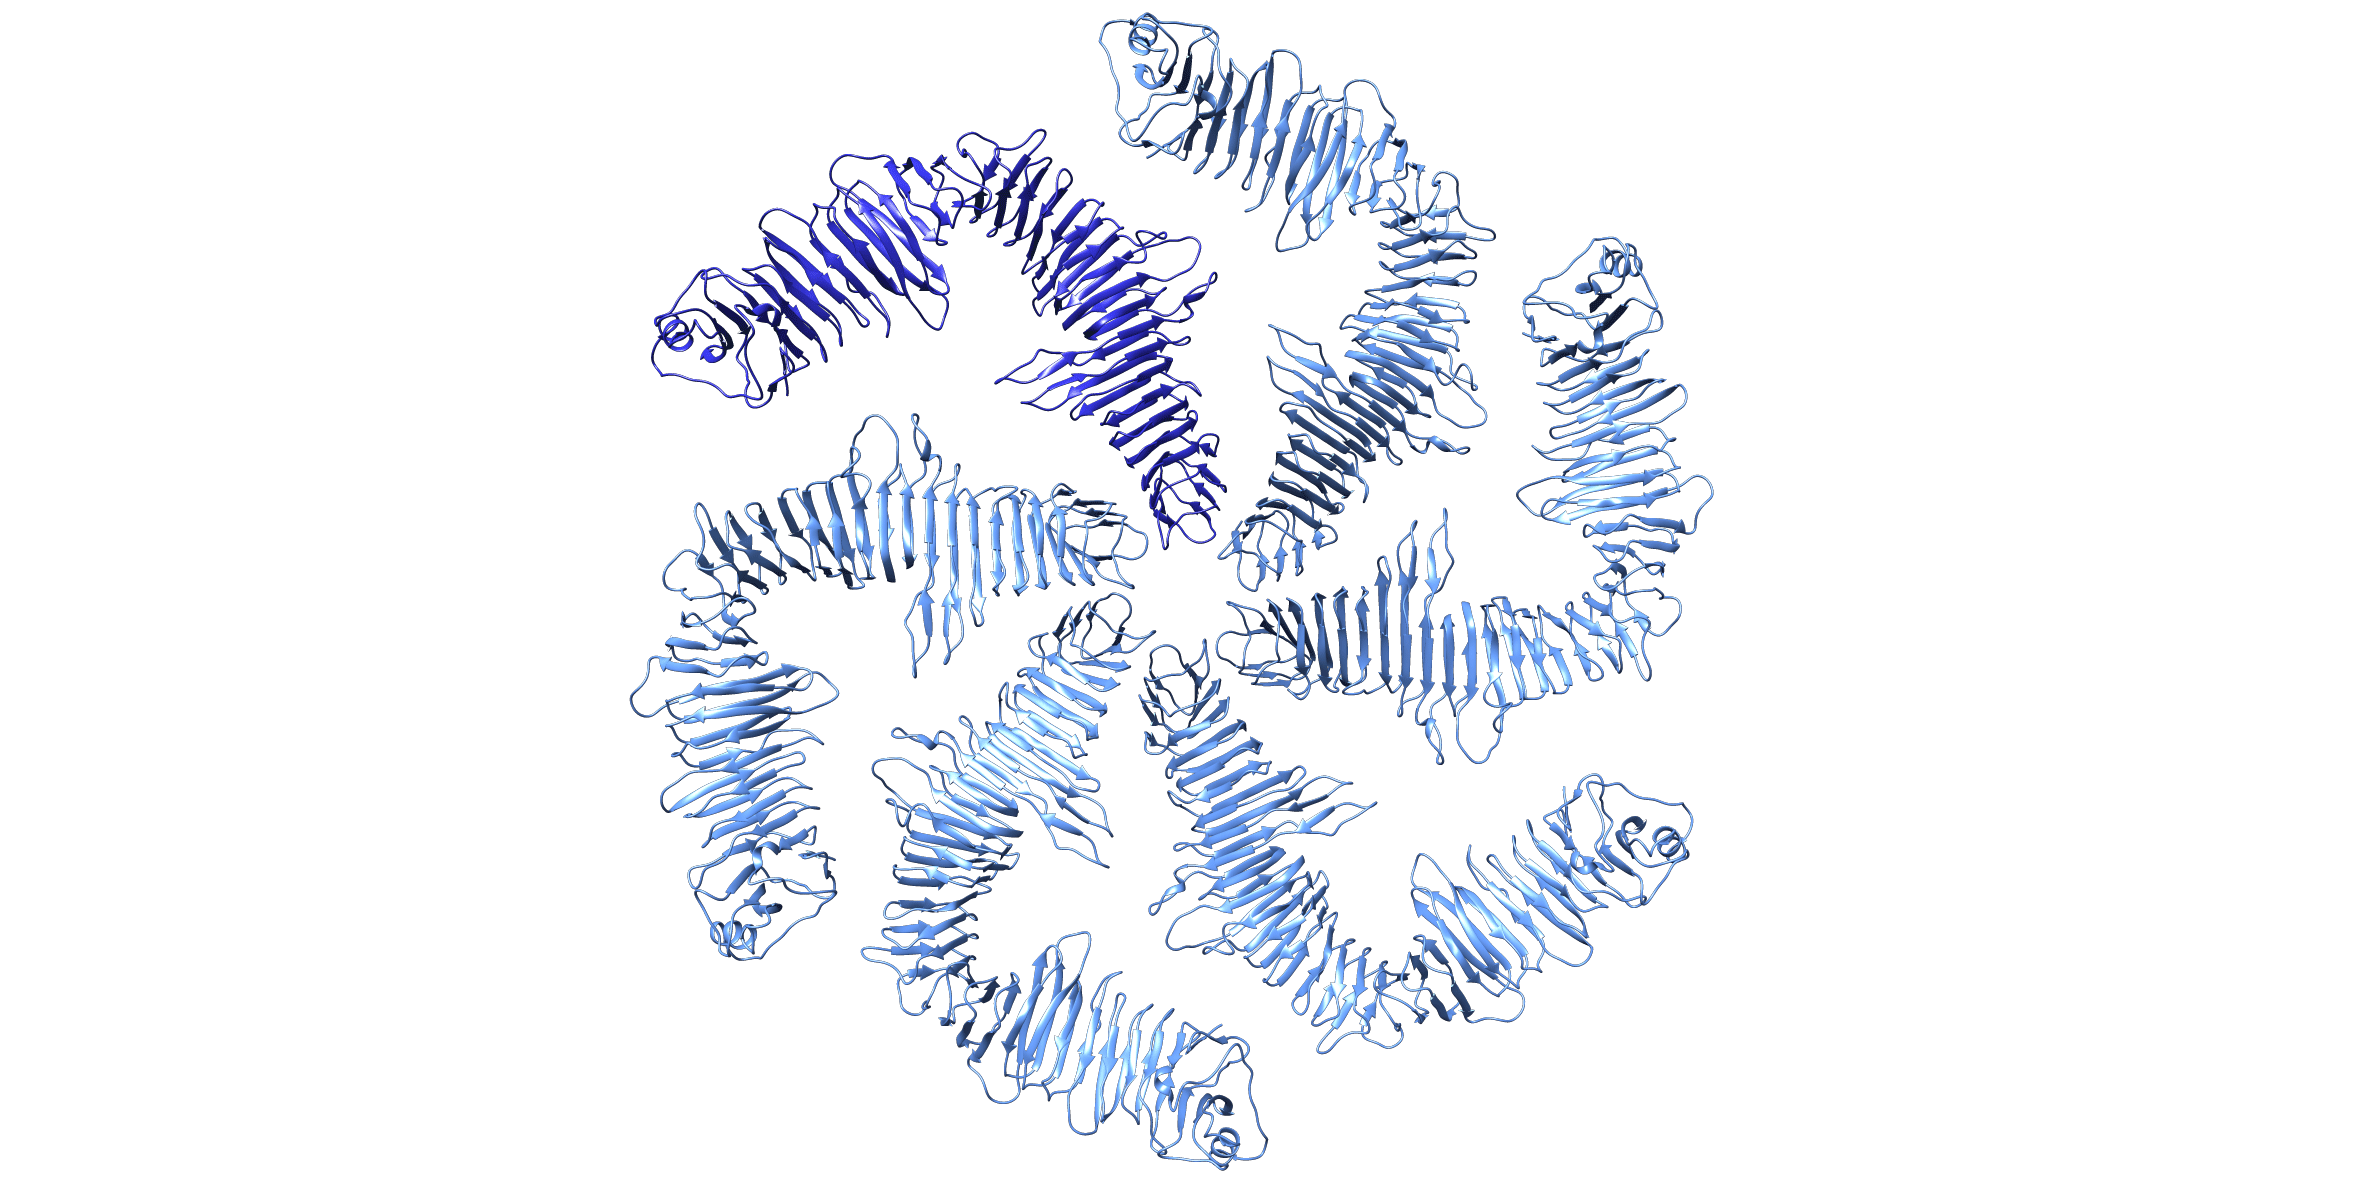
\includegraphics{img/schematics/2_6_1}

\href{http://rcsb.org/structure/5N97}{\emph{PDB: 5N97}}
A single protein forms the surface layer you just saw in \emph{Caulobacter crescentus}. The protein has two domains. The bottom domain anchors it to lipoproteins attached to the outer membrane. The top domain forms the canopy of the S-layer, organizing hierarchically into hexameric rosettes like this which in turn pack into a larger hexameric lattice \citep{bharat2017}. This lattice is flexible enough to curve around even narrow regions of the cell like the stalk discussed in Chapter 3.

\hypertarget{Nanopods}{%
\subsection*{More: Nanopods}\label{Nanopods}}
\addcontentsline{toc}{subsection}{More: Nanopods}

Archaea and bacteria with surface layers produce characteristic outer membrane vesicles: they bud off with the surface layer attached. You will see plenty of examples in the coming pages. \emph{Delftia acidovorans} like this produce so-called nanopods: chains of outer membrane vesicles ensheathed in surface layer.



\hypertarget{htmlwidget-f0420dc727b02c8bec6e}{}

\label{fig:2-6a}\protect\hyperlink{tree}{Delftia acidovorans} Collected by: \protect\hyperlink{elitza_tocheva}{Elitza Tocheva} Movie DOI: \href{https://doi.org/10.22002/D1.1366}{10.22002/D1.1366}

\hypertarget{surface-layer-variety}{%
\section{Surface Layer Variety}\label{surface-layer-variety}}

One of the most striking features of the surface layer is how different it can look in different species. For instance, compare this archaeal \emph{Sulfolobus solfataricus} cell to the bacterium on the last page, or to other diderm \protect\hyperlink{Methylomicrobium_alcaliphilum}{More: Methylomicrobium alcaliphilum} or monoderm \protect\hyperlink{Clostridium_thermocellum}{More: Clostridium thermocellum} bacteria, or archaea \protect\hyperlink{Nitrosopumilus_maritimus}{More: Nitrosopumilus maritimus}; \protect\hyperlink{Methanoregula_formicica}{More: Methanoregula formicica}. All surface layers are crystalline lattices of a single--or in a few cases, two--proteins, but the particular pattern of the lattice depends on the shape of this building block and how it multimerizes into a higher-order structure. The shape of the building block varies considerably; there is almost no sequence homology between S-layer proteins from different species. And shapes come together in different ways, forming repeating units of one, two, three (as on this cell), four, or six blocks.

S-layers are very common in archaea like this \emph{S. solfataricus}. Most archaea lack cell walls, so the surface layer functions as external scaffolding. Remember, too, that nearly all archaea are monoderms, lacking the extra periplasmic compartment that diderms have. Here again the surface layer serves a similar function, enclosing a space around the cell's membrane called the pseudo-periplasmic space. Just as with the bacterial periplasm, this space serves as an antechamber for the cell, restricting access by large molecules. In some cases, the pseudo-periplasmic space also contains proteins that function in metabolism.



\hypertarget{htmlwidget-2ca4060c2f8246ed941c}{}

\label{fig:2-7}\protect\hyperlink{tree}{Sulfolobus solfataricus} Collected by: \protect\hyperlink{lu_gan}{Lu Gan} Movie DOI: \href{https://doi.org/10.22002/D1.1356}{10.22002/D1.1356}

\hypertarget{Methylomicrobium_alcaliphilum}{%
\subsection*{More: Methylomicrobium alcaliphilum}\label{Methylomicrobium_alcaliphilum}}
\addcontentsline{toc}{subsection}{More: Methylomicrobium alcaliphilum}

In \emph{Methylomicrobium alcaliphilum}, V-shaped surface layer proteins come together to form cups that pack into a hexagonal pattern.



\hypertarget{htmlwidget-1836bccf1e84fb05ec60}{}

\label{fig:2-7a}\protect\hyperlink{tree}{Methylomicrobium alcaliphilum} Collected by: \protect\hyperlink{songye_chen}{Songye Chen} Movie DOI: \href{https://doi.org/10.22002/D1.1367}{10.22002/D1.1367}

\hypertarget{Clostridium_thermocellum}{%
\subsection*{More: Clostridium thermocellum}\label{Clostridium_thermocellum}}
\addcontentsline{toc}{subsection}{More: Clostridium thermocellum}

Not only diderm bacteria have surface layers, as you can see on this monoderm \emph{Clostridium thermocellum} cell. The main difference is that the proteins are anchored to the cell wall, rather than to the outer membrane (or associated lipoproteins).



\hypertarget{htmlwidget-1459161d99c8950ecfb9}{}

\label{fig:2-7b}\protect\hyperlink{tree}{Clostridium thermocellum} Collected by: \protect\hyperlink{william_nicolas}{William Nicolas} Movie DOI: \href{https://doi.org/10.22002/D1.1476}{10.22002/D1.1476}

\hypertarget{Nitrosopumilus_maritimus}{%
\subsection*{More: Nitrosopumilus maritimus}\label{Nitrosopumilus_maritimus}}
\addcontentsline{toc}{subsection}{More: Nitrosopumilus maritimus}

In \emph{Nitrosopumilus maritimus}, surface layer proteins form hexagonal rosettes that in turn pack into a hexagonal lattice.



\hypertarget{htmlwidget-ec5b118c2a8213827a0d}{}

\label{fig:2-7c}\protect\hyperlink{tree}{Nitrosopumilis maritimus} Collected by: \protect\hyperlink{rasika_ramdasi}{Rasika Ramdasi} Movie DOI: \href{https://doi.org/10.22002/D1.1368}{10.22002/D1.1368}

\hypertarget{Methanoregula_formicica}{%
\subsection*{More: Methanoregula formicica}\label{Methanoregula_formicica}}
\addcontentsline{toc}{subsection}{More: Methanoregula formicica}

The surface layer of \emph{Methanoregula formicica} is a hexagonal lattice of small, nearly circular subunits.



\hypertarget{htmlwidget-38a56b914518f77a8529}{}

\label{fig:2-7d}\protect\hyperlink{tree}{Methanoregula formicica} Collected by: \protect\hyperlink{ariane_briegel}{Ariane Briegel} Movie DOI: \href{https://doi.org/10.22002/D1.1369}{10.22002/D1.1369}

\hypertarget{sheath}{%
\section{Sheath}\label{sheath}}

Why stop at a single layer of protein? For proof that Nature is endlessly inventive, consider this \emph{Methanospirillum hungatei} cell. These archaea encase themselves in a surface layer, as well as an additional protein layer that forms a highly impermeable sheath. The sheath is also very resistant to pressure, which could be important in these cells' line of work. \emph{M. hungatei} were discovered in sewage, where they break down organic waste, producing methane. One theory is that the sheath acts as a pressure regulator; when enough methane builds up inside the cell, the pressure expands the sheath, opening its pores wide enough to allow the methane to dissipate and new metabolic substrates like hydrogen and carbon dioxide to enter.

The rules of architecture remain the same, though. Just as in the bacterial cell wall, sheath polymers are arranged as hoops perpendicular to the long axis of the rod-shaped cell. At the ends of the sheath, multiple protein layers stack into a thick plug. Cells divide within the sheath, and long chains of cells in a continuous sheath are often observed.



\hypertarget{htmlwidget-679af4ef716d3046dff3}{}

\label{fig:2-8}\protect\hyperlink{tree}{Methanospirillum hungatei} Collected by: \protect\hyperlink{ariane_briegel}{Ariane Briegel} Movie DOI: \href{https://doi.org/10.22002/D1.1357}{10.22002/D1.1357}

\hypertarget{dna}{%
\section{DNA}\label{dna}}

All the layers we just discussed collectively make up the container, or envelope, of a cell. As you have seen, different species use different combinations of these components to form their envelopes; the only constant is the cytoplasmic (or inner, for diderms) membrane.

Now consider what these envelopes contain. In addition to water and small molecules, you have already seen some large protein complexes like motility machines. You have also seen many ribosomes--the protein/RNA complexes responsible for translating RNA into proteins. But you might have been surprised \emph{not} to see something else: deoxyribonucleic acid, or DNA. The molecule containing the instructions for the life of the cell is of paramount importance, yet often invisible by microscopy. But not always. Thin filaments of DNA, only about 2 nm wide, blend in with the dense cytoplasm of the cell. When a cell lyses, though, its cytoplasm diffuses into the environment and the DNA filaments stand out against the now-much-reduced background. You can get an idea of the sheer abundance of DNA inside a cell from this \emph{Haloarcula argentinensis} whose envelope has ruptured and contents are spilling out.



\hypertarget{htmlwidget-469fea7074dd11c065e7}{}

\label{fig:2-9}\protect\hyperlink{tree}{Haloarcula argentinensis} Collected by: \protect\hyperlink{ariane_briegel}{Ariane Briegel} Movie DOI: \href{https://doi.org/10.22002/D1.1358}{10.22002/D1.1358}

\hypertarget{nucleoid}{%
\section{Nucleoid}\label{nucleoid}}

Cells contain enormous amounts of DNA. The single, circular chromosome of this \emph{Bdellovibrio bacteriovorus} cell contains 3,782,950 individual nucleotide pairs, which means that if the circle were cut and laid out as a long piece, it would be about \emph{one thousand times} longer than the cell itself. To fit and function inside the cell, the chromosome has to be extraordinarily organized and packed, a feat we still do not understand. Some of this packing is evident in nearly every cell: the center of the cell tends to have very few large macromolecular complexes like ribosomes, because they are excluded by the densely-packed chromosome(s). Look for these ribosome-excluding zones in the rest of the book; they indicate the location of the bulk of the cell's DNA. Since this region is not enclosed by an internal membrane, it is not called a nucleus (the ``karyon'' that defines eukaryotes). Instead, we use the term nucleoid to describe the cytoplasmic region where most of the DNA is concentrated.

At times, the nucleoid becomes easier to see. Imagine that your cell wanted to decrease its gene expression (we will discuss why in Chapters 8 and 9). One approach is simply to pack the chromosome so tightly that the transcriptional machinery cannot access the genes. This cell is doing just that, condensing its nucleoid into a dense twisted braid we can easily visualize.



\hypertarget{htmlwidget-5eb68b05192fb5be2005}{}

\label{fig:2-10}\protect\hyperlink{tree}{Bdellovibrio bacteriovorus} Collected by: \protect\hyperlink{yi-wei_chang}{Yi-Wei Chang} Movie DOI: \href{https://doi.org/10.22002/D1.1359}{10.22002/D1.1359}

\hypertarget{further-reading-1}{%
\section{Further Reading}\label{further-reading-1}}

Errington (2013). \emph{L-form bacteria, cell walls and the origins of life} \citep{errington2013}.

Ptacin and Shapiro (2013). \emph{Chromosome architecture is a key element of bacterial cellular organization} \citep{ptacin2013}.

Sleytr and Beveridge (1999). \emph{Bacterial S-layers} \citep{sleytr1999}.

Strahl and Errington (2017). \emph{Bacterial membranes: Structure, domains, and function} \citep{strahl2017}.

\hypertarget{shape}{%
\chapter{Shape}\label{shape}}

\begin{quote}
``To be brutally honest, few people care that bacteria have different shapes. Which is a shame, because the bacteria seem to care very much.''
- Kevin Young \citep{young2006}
\end{quote}

\hypertarget{coccoid}{%
\section{Coccoid}\label{coccoid}}

What kind of life do you envision for your cell? Just as the design of buildings reflects their purpose, different cell shapes suit different lifestyles. Does your cell need to soak up sunlight for photosynthesis? Burrow through the tissue of a host? Chase down prey? Each lifestyle is best served by a particular form.

How can you give your cell a particular form? The final shape of a building is determined by a shell erected around a system of internal beams and joists--its skeleton. Cells determine their shape using a similar system--the rigid exoskeleton of the cell wall and/or surface layer in concert with an internal cyto(``cell'')-skeleton. The cytoskeleton of bacteria and archaea comprises a set of proteins that form filaments or other superstructures that move or scaffold other material in the cell. In many cases, this cytoskeletal scaffolding is dynamic and ever-changing, appropriate for a living building.

Consider a cell like this \emph{Simkania negevensis}. It takes the form of a sphere--the default shape for a membrane in water, uniformly resistant to pressure, and the best shape if you want to maximize your volume relative to surface area. We refer to spherical cells as coccoid (``berry-like''). To grow, a coccoid cell can simply add lipids to its membrane(s) and randomly insert new glycan strands into its cell wall, expanding to a larger radius.



\hypertarget{htmlwidget-e8e61f6b0f26428609b0}{}

\label{fig:3-1}\protect\hyperlink{tree}{Simkania negevensis} Collected by: \protect\hyperlink{martin_pilhofer}{Martin Pilhofer} Movie DOI: \href{https://doi.org/10.22002/D1.1477}{10.22002/D1.1477}

\hypertarget{rod}{%
\section{Rod}\label{rod}}

Instead of a sphere, maybe you would like to make your cell cylindrical, like this \emph{Cupriavidus necator}. Rod-shaped cells (cylinders with hemispherical caps) are a very common form for bacteria and archaea, likely because they are efficient swimmers and swarmers (more on that in Chapter 6). Starting from a sphere, imagine that you had a construction contractor who could direct where workers lay in new cell wall. Instead of random insertion, you could, say, direct them to work around a single plane. As the workers laid in more and more hoops of peptidoglycan in this region, a cylinder would form with the same diameter as the initial sphere (which would now serve as the structure's end caps).

The contractor for most rod-shaped bacterial cells is a cytoskeletal protein named MreB, which is a homolog of the eukaryotic cytoskeletal protein actin. It remains unclear exactly how it works (cryoET imaging debunked a once-leading theory), but small patches of MreB seem to shuttle rapidly around the circumference of the cell, directing where the proteins you saw in the last chapter add new peptidoglycan to the sacculus. MreB's circuit is restricted to the cylindrical portion of the cell, expanding the rod without affecting the ends. This growth pattern has an interesting consequence: the peptidoglycan in the cell caps is older than the peptidoglycan in the cylindrical center. The two types, old and new, can thus serve as convenient landmarks, for instance allowing the cell to tether something to the end.

Not all rod-shaped bacteria use MreB, and we are still figuring out how the shape forms in many species \protect\hyperlink{Rod_variety}{More: Rod variety}. For rod-shaped archaea \protect\hyperlink{Archaeal_rods}{More: Archaeal rods}, the surface layer plays an important role in determining the shape.



\hypertarget{htmlwidget-fb70761d92ff3184dfd3}{}

\label{fig:3-2}\protect\hyperlink{tree}{Cupriavidus necator} Collected by: \protect\hyperlink{morgan_beeby}{Morgan Beeby} Movie DOI: \href{https://doi.org/10.22002/D1.1478}{10.22002/D1.1478}

\hypertarget{Rod_variety}{%
\subsection*{More: Rod variety}\label{Rod_variety}}
\addcontentsline{toc}{subsection}{More: Rod variety}

Not all rod-shaped cells are perfectly cylindrical. For instance, \emph{Brucella abortus} like this one are pear-shaped. This is one of the rod-shaped bacterial species that do not use MreB.



\hypertarget{htmlwidget-e0511119af84a14bcea4}{}

\label{fig:3-2a}\protect\hyperlink{tree}{Brucella abortus} Collected by: \protect\hyperlink{ariane_briegel}{Ariane Briegel} Movie DOI: \href{https://doi.org/10.22002/D1.1484}{10.22002/D1.1484}

\hypertarget{Archaeal_rods}{%
\subsection*{More: Archaeal rods}\label{Archaeal_rods}}
\addcontentsline{toc}{subsection}{More: Archaeal rods}

Some archaeal species, like this \emph{Methanoregula formicica}, are rod-shaped. The rigid surface layer seems to help define the shape, but the details are still unknown.



\hypertarget{htmlwidget-c9804181743554eea2e4}{}

\label{fig:3-2b}\protect\hyperlink{tree}{Methanoregula formicica} Collected by: \protect\hyperlink{ariane_briegel}{Ariane Briegel} Movie DOI: \href{https://doi.org/10.22002/D1.1485}{10.22002/D1.1485}

\hypertarget{length}{%
\section{Length}\label{length}}

Rod-shaped cells have a useful property: they can grow by extending their length without significantly changing the ratio of their surface area to volume, which would in turn change how efficiently they can take up nutrients from the environment. This property enables an impressive range of lengths for rod-shaped cells, from the short \emph{Cupriavidus necator} you just saw, to this much longer \emph{Hylemonella gracilis}.

The length of a cell (or, more generally, its size) varies depending on the environment or its stage of the lifecycle, but it does not vary much. Size tends to be strongly conserved within a species, ranging not much more than the factor of two dictated by replication. Sizes \emph{between} species vary much more widely, as you will see throughout this book. Keep in mind, too, that the species we are able to image directly by cryoET are relatively small. Other species can be much larger, in some exceptional cases up to 100 µm across.



\hypertarget{htmlwidget-94376f1ef010ecc840a7}{}

\label{fig:3-3}\protect\hyperlink{tree}{Hylemonella gracilis} Collected by: \protect\hyperlink{yi-wei_chang}{Yi-Wei Chang} Movie DOI: \href{https://doi.org/10.22002/D1.1479}{10.22002/D1.1479}

\hypertarget{vibrioid}{%
\section{Vibrioid}\label{vibrioid}}

What if you want to curve your rod-shaped cell into a comma? Vibrioid shape (named for the genus \emph{Vibrio}, where it is common) may help cells swim faster. For \emph{Caulobacter crescentus} like this one, it also helps them stay close to a surface as liquid flows past, increasing the chance that their progeny can attach before they are swept away. To make a vibrioid cell wall, you can imagine the contractor simply telling the workers to incorporate more material on one side of the rod relative to the other. In \emph{C. crescentus}, this is the function of two cytoskeletal proteins. The first, called (for an obvious reason) Crescentin, inhibits cell wall synthesis. It is kept in check by the second, called CTP synthase. (As its name implies, CTP synthase has another, metabolic, function in the cell \protect\hyperlink{CTP_synthase}{Schematic: CTP synthase}.) The balance between the two makes sure the cell curves, but not too much. Such checks and balances are a common theme in Nature. Both cytoskeletal proteins localize to one side of the cell, resulting in more cell wall growth on the opposite side, and a curved cell. Here you can see a bundle of CTP synthase filaments on the inner curvature of the cell. The form of Crescentin is more elusive; we only see obvious filaments when it is artificially overexpressed, so its exact structure in the cell remains unclear.

This system is only one way of making a curved cell. There must be others since many vibrioid species (including \emph{Vibrio}!) do not use Crescentin. As you will see throughout this book, there is no shortage of biological questions still to be figured out.



\hypertarget{htmlwidget-95d8db3b9d52493953a0}{}

\label{fig:3-4}\protect\hyperlink{tree}{Caulobacter crescentus} Collected by: \protect\hyperlink{prabha_dias}{Prabha Dias} Movie DOI: \href{https://doi.org/10.22002/D1.1480}{10.22002/D1.1480}

\hypertarget{CTP_synthase}{%
\subsection*{Schematic: CTP synthase}\label{CTP_synthase}}
\addcontentsline{toc}{subsection}{Schematic: CTP synthase}

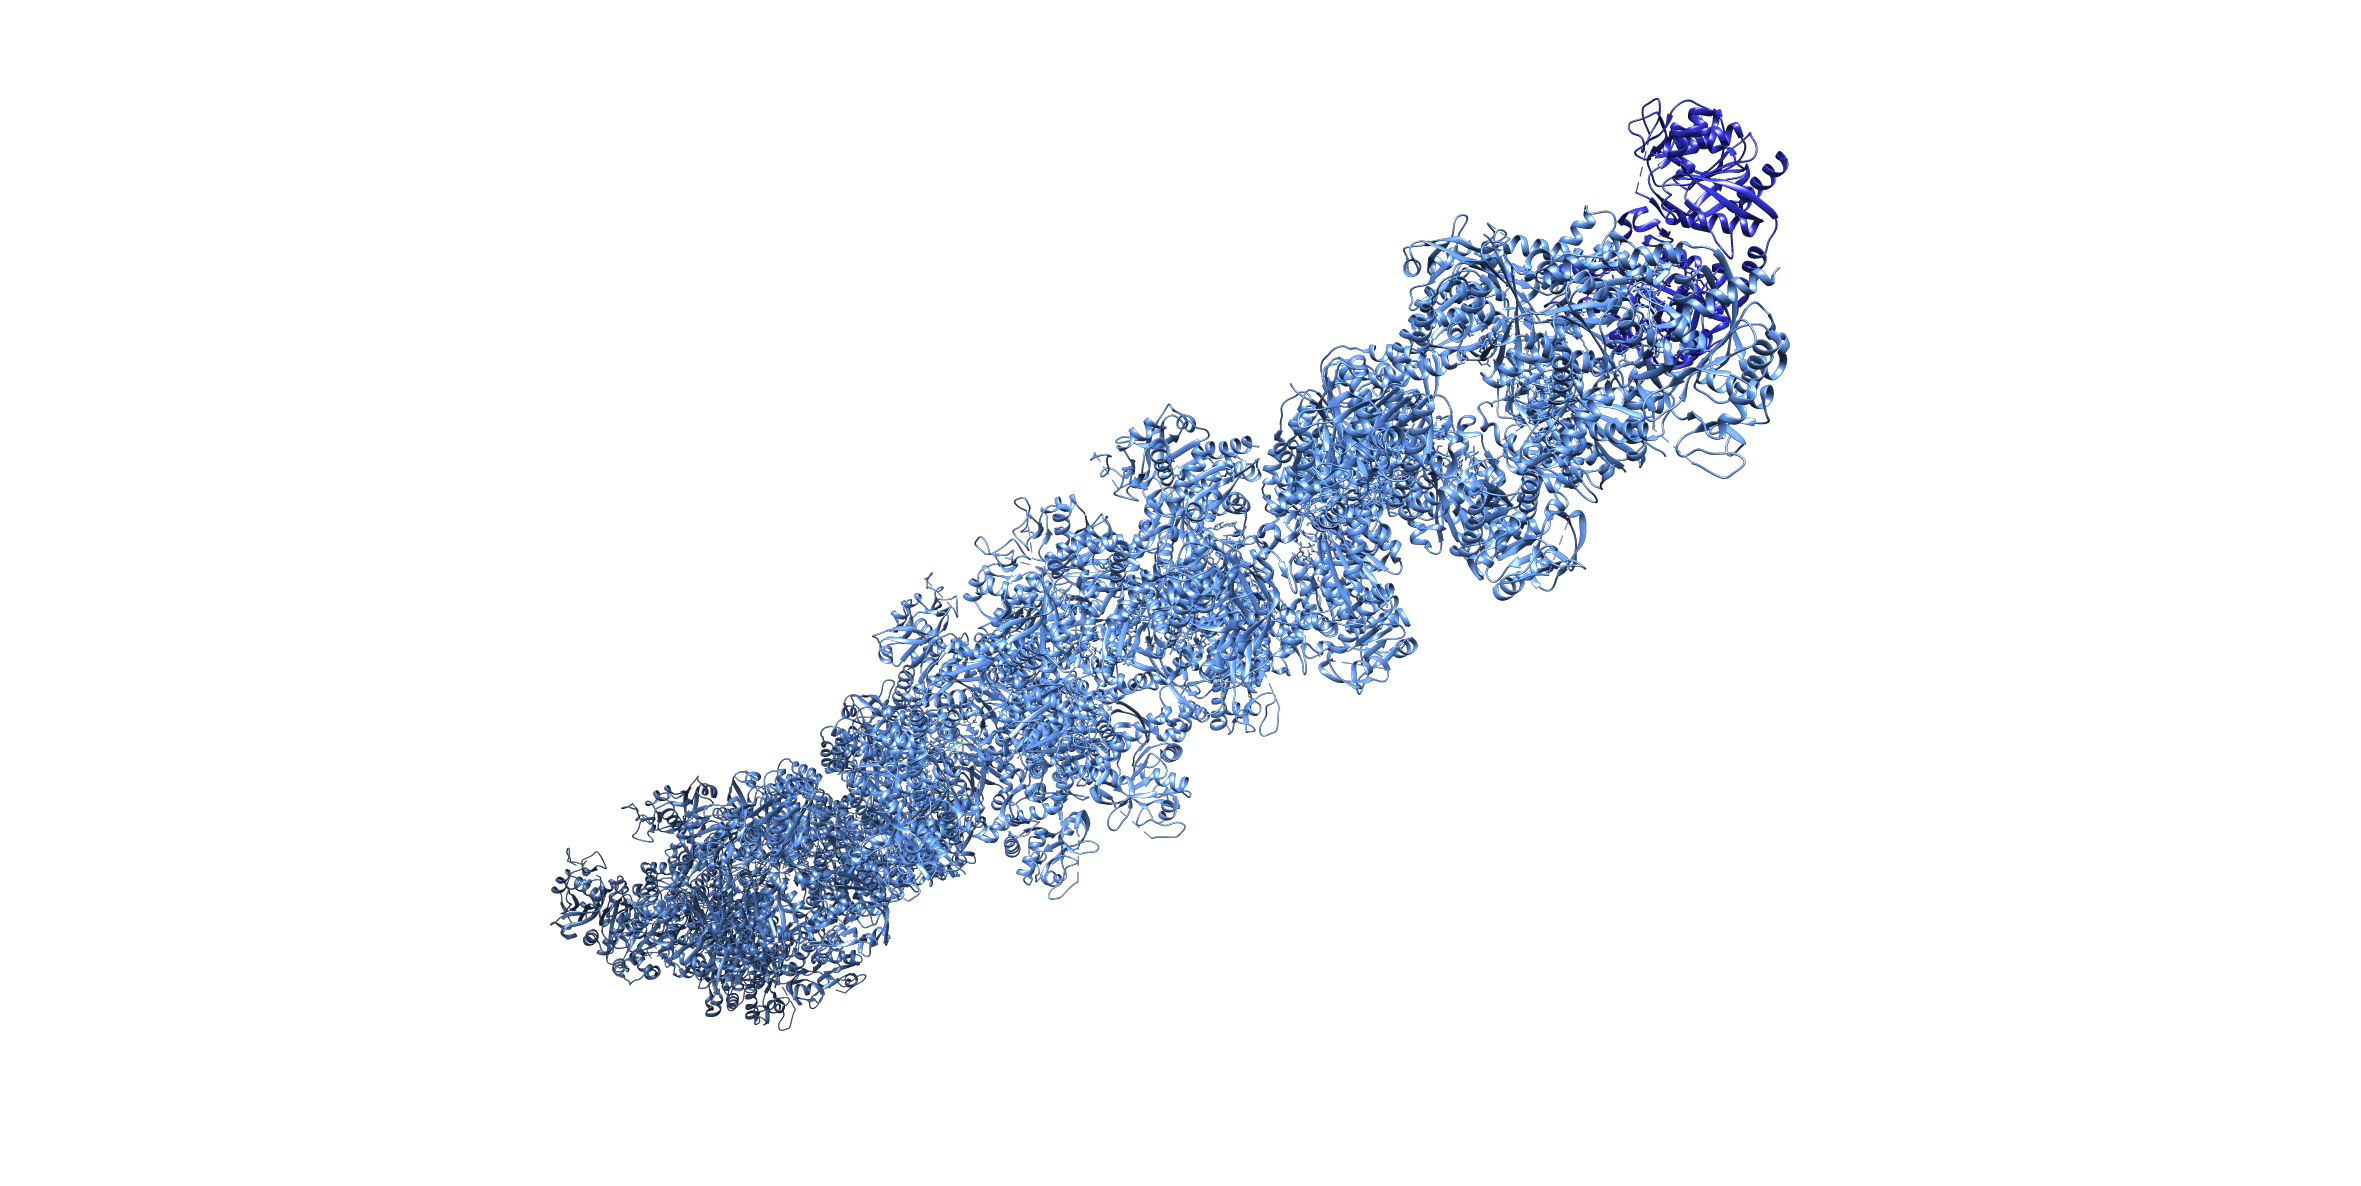
\includegraphics{img/schematics/3_4_1}

\href{http://rcsb.org/structure/5U3C}{\emph{PDB: 5U3C}}
CTP synthase is a fundamental metabolic protein across all domains of life, helping make the building blocks of RNA and DNA. It also polymerizes into filaments. In eukaryotes, the filament structure activates the enzyme. In bacteria, the filament structure (shown here for \emph{Escherichia coli} \citep{lynch2017}) inhibits the enzyme's metabolic function. Polymerization of enzymes is fairly common, providing an elegant way to quickly regulate the activity of a protein that may not always be needed, but would be costly or slow to degrade and synthesize again. You will see another example in Chapter 4. In the case of CTP synthase, the cytoskeletal role likely arose secondarily; once you have a long filament lying around, why not use it as a scaffold?

\hypertarget{helical}{%
\section{Helical}\label{helical}}

Why stop at a quarter turn when you can twist your cell into a full wave or even a corkscrew? Just as a corkscrew penetrates its target, helical pathogenic bacteria like this \emph{Campylobacter jejuni} can burrow efficiently into the tissue of their target.

It can be tempting to group species based on a common characteristic, but appearances are often deceiving about relatedness. Undulating shape, for instance, was not a one-shot invention; it evolved independently multiple times. This is true of other bacterial and archaeal cell shapes as well. For wavy shape, these independent origins are reflected in different mechanisms of creating it. Some species, including \emph{C. jejuni}, use dedicated proteins to regulate the pattern of peptidoglycan insertion--a continuation of the theme we've been discussing. Other species take different approaches \protect\hyperlink{Borrelia_burgdorferi}{More: Borrelia burgdorferi}.



\hypertarget{htmlwidget-11c4bcb0221e3fe34537}{}

\label{fig:3-5}\protect\hyperlink{tree}{Campylobacter jejuni} Collected by: \protect\hyperlink{morgan_beeby}{Morgan Beeby} Movie DOI: \href{https://doi.org/10.22002/D1.1481}{10.22002/D1.1481}

\hypertarget{Borrelia_burgdorferi}{%
\subsection*{More: Borrelia burgdorferi}\label{Borrelia_burgdorferi}}
\addcontentsline{toc}{subsection}{More: Borrelia burgdorferi}

\emph{Borrelia burgdorferi} like this cell use the long filaments of their motility machinery (flagella, discussed in Chapter 6) as a kind of cytoskeleton. A bundle of flagella wraps around the cell in the periplasm, between the cell wall and the outer membrane. Spun by motors at their base (more on that in Chapter 6), the filaments impart a wave pattern to the growing sacculus. Without the motors' rotation, the cells develop a rod shape. Note that \emph{B. burgdorferi} are not helical, but rather adopt a two-dimensional waveform.



\hypertarget{htmlwidget-b69f659f341ba3286bc3}{}

\label{fig:3-5a}\protect\hyperlink{tree}{Borrelia burgdorferi} Collected by: \protect\hyperlink{ariane_briegel}{Ariane Briegel} Movie DOI: \href{https://doi.org/10.22002/D1.1486}{10.22002/D1.1486}

\hypertarget{prosthecate}{%
\section{Prosthecate}\label{prosthecate}}

Motility is not everything. Another major force that shapes cells is metabolism. Nutrients are often scarce, and increasing your cell's ability to absorb them can give it a boost in the competitive game of life. So how can you do that? Remember that a sphere maximizes volume relative to surface area. To maximize surface area (for nutrient uptake) relative to volume, you would instead want something spikier. Some bacteria extend prosthecae (``add-ons'' or appendages) for this purpose. Some, like \emph{Caulobacter crescentus}, use a single prostheca, which is also called a stalk. Stalks are commonly located at the pole of the cell, where, as you'll see in Chapter 8, they can help cells attach to a surface and hang on even in turbulent flow in the freshwater lakes and streams where they live. Other species have a stalk on either end. Still others, like this \emph{Verrucomicrobium spinosum}, form astral shapes with prosthecae jutting out in all directions.

Prosthecae offer a challenge for the architect: thin extensions are delicate. Prosthecate cells use cytoskeletal proteins to form and stabilize their stalks, although exactly how this works remains unclear. One of these cytoskeletal proteins is Bactofilin \protect\hyperlink{Bactofilin}{Schematic: Bactofilin}, which is similar to the proteins that make intermediate filaments in eukaryotes. \emph{C. crescentus} use Bactofilin polymers to help make their stalks. \emph{Prosthecobacter} contain a different cytoskeletal element--microtubules--in their stalks, the function of which remains unclear \protect\hyperlink{Bacterial_microtubules}{More: Bacterial microtubules}.



\hypertarget{htmlwidget-cbb4e48926886e653aef}{}

\label{fig:3-6}\protect\hyperlink{tree}{Verrucomicrobium spinosum} Collected by: \protect\hyperlink{martin_pilhofer}{Martin Pilhofer} Movie DOI: \href{https://doi.org/10.22002/D1.1482}{10.22002/D1.1482}

\hypertarget{Bactofilin}{%
\subsection*{Schematic: Bactofilin}\label{Bactofilin}}
\addcontentsline{toc}{subsection}{Schematic: Bactofilin}

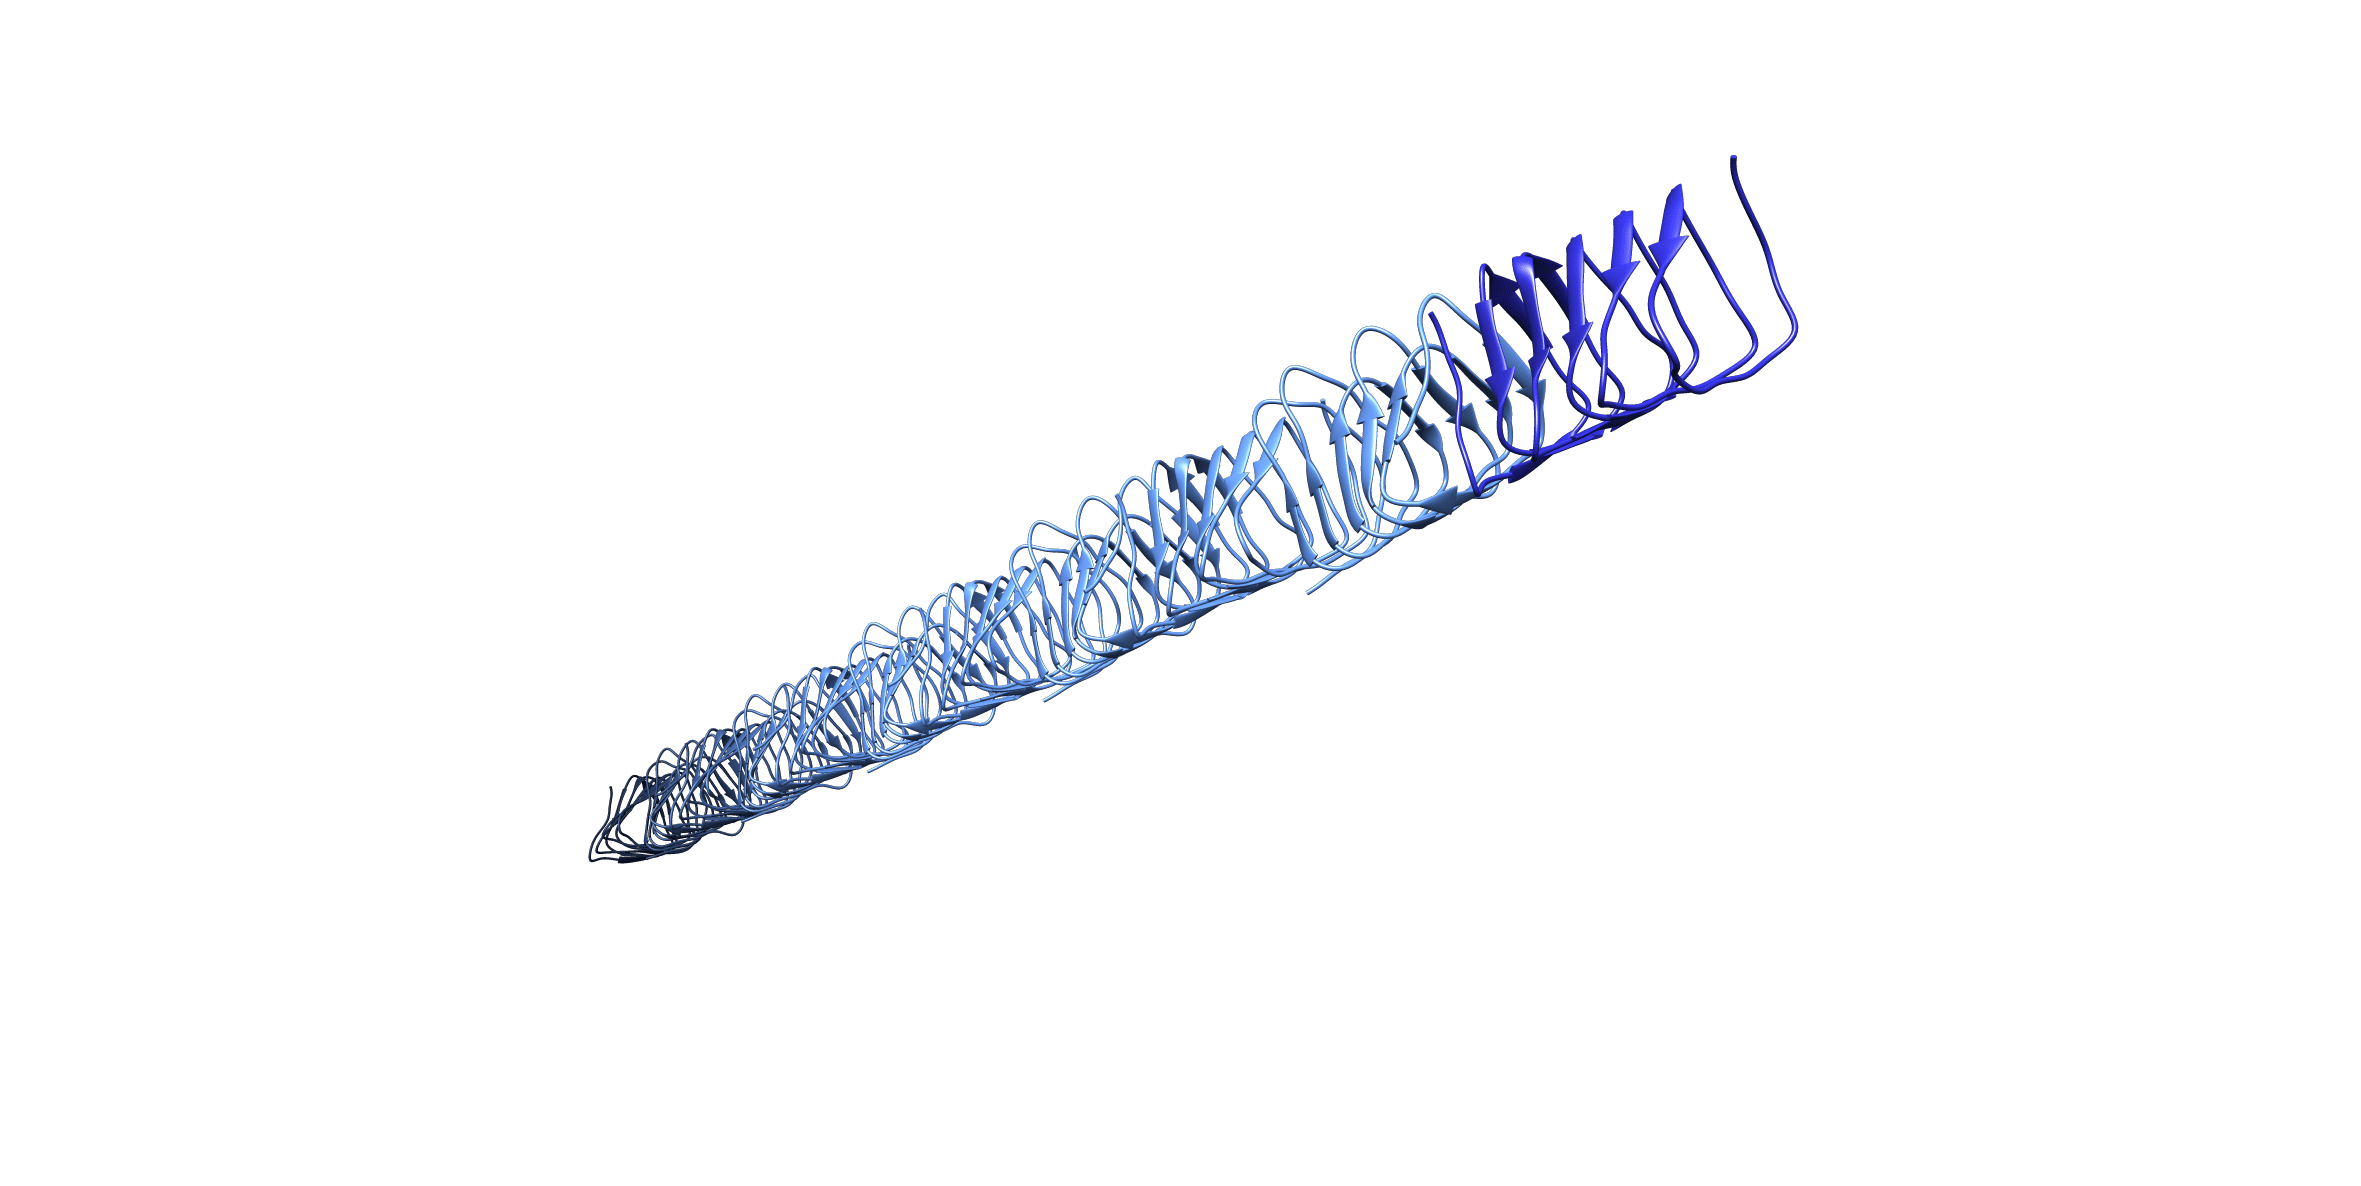
\includegraphics{img/schematics/3_6_1}

\href{http://rcsb.org/structure/6RIB}{\emph{PDB: 6RIB}}
Bactofilins are found in many species of bacteria and archaea, suggesting that they perform diverse (and currently unknown) functions. They polymerize into very stable filaments with a triangular beta-helical structure, like this one from \emph{Thermus thermophilus} \citep{deng2019}. Bactofilin filaments lack two hallmarks of actin- and tubulin-based cytoskeletal elements: polarity and dynamic assembly/disassembly. In this way, they are similar to intermediate filaments in eukaryotic cytoskeletons.

\hypertarget{Bacterial_microtubules}{%
\subsection*{More: Bacterial microtubules}\label{Bacterial_microtubules}}
\addcontentsline{toc}{subsection}{More: Bacterial microtubules}

Some bacterial species with prosthecae express structures similar to eukaryotic microtubules, made from two proteins called BtubA and BtubB to reflect their homology to eukaryotic tubulins. Eukaryotic microtubules are hollow tubes formed by 13 protofilaments; bacterial microtubules are smaller, with only \textasciitilde{}5 protofilaments. Cells commonly contain a bundle of microtubules in their prosthecae, like this \emph{Prosthecobacter vanneervenii} cell, which has a bundle of four.

\emph{Prosthecobacter} belong to an evolutionarily unique group of species that share characteristics unusual in the rest of the bacterial phylogenetic tree. We refer to the collective group as the PVC superphylum (because it contains \emph{Planctomycetes}, \emph{Verrucomicrobia}, and \emph{Chlamydiae}). Having homologs of eukaryotic microtubule proteins is one of these unique characteristics; so far, Btubs have only been identified in species of \emph{Prosthecobacter}. They seem to have come from a horizontal gene transfer from a eukaryotic cell (meaning that microtubules evolved first in eukaryotes and were later borrowed by the bacteria).



\hypertarget{htmlwidget-c169885ba2dde106f578}{}

\label{fig:3-6a}\protect\hyperlink{tree}{Prosthecobacter vanneervenii} Collected by: \protect\hyperlink{martin_pilhofer}{Martin Pilhofer} Movie DOI: \href{https://doi.org/10.22002/D1.1487}{10.22002/D1.1487}

\hypertarget{square}{%
\section{Square}\label{square}}

So far we have focused on bacteria, but archaea hold their own in the specialized shape competition. In fact, one of the most extreme examples of maximizing surface area relative to volume comes from this archaeon, \emph{Haloquadratum walsbyi}, which grows as thin, square tiles. \emph{Very} thin, square tiles. This property helps keep them oriented with their broad sides to the sun, whose light they rely on for photosynthesis. Gas vesicles \protect\hyperlink{Gas_vesicles}{More: Gas vesicles} keep the cells buoyant in the super-salty lakes where they live.

We still do not know exactly how this shape is determined, but at least part of the mechanism seems to involve glycoproteins on the cell's surface layer.



\hypertarget{htmlwidget-c85ca4ebbc0f17c73b52}{}

\label{fig:3-7}\protect\hyperlink{tree}{Haloquadratum walsbyi} Collected by: \protect\hyperlink{zhuo_li}{Zhuo Li} Movie DOI: \href{https://doi.org/10.22002/D1.1483}{10.22002/D1.1483}

\hypertarget{Gas_vesicles}{%
\subsection*{More: Gas vesicles}\label{Gas_vesicles}}
\addcontentsline{toc}{subsection}{More: Gas vesicles}

Some species of archaea and bacteria use gas vesicles to control their buoyancy. This can allow them to rise or fall in a water column, which can be a great advantage. \emph{Halobacterium salinarum} like this one produce gas vesicles in response to cues from the environment, lifting themselves out of the sediment and into more favorable conditions of oxygen or sunlight for photosynthesis. This cell has just started producing gas vesicles, so they are small and isolated. Later, the vesicles will elongate into cylinders with conical ends, as you saw in \emph{Haloquadratum walsbyi}. Each cell might contain dozens of vesicles, and they often cluster together.

Gas vesicles are microcompartments enclosed by a hydrophobic shell made of a single layer of protein. (Sometimes some additional proteins reinforce the shell.) Gas vesicles do not actively store gas; they simply allow gas dissolved in the cytoplasm to diffuse in, while forming a tight barrier against anything else, like water. They are fragile and prone to collapse with even a slight increase in the surrounding pressure.



\hypertarget{htmlwidget-9c10993e1e9ecc62bdd3}{}

\label{fig:3-7a}\protect\hyperlink{tree}{Halobacterium salinarum} Collected by: \protect\hyperlink{ariane_briegel}{Ariane Briegel} Movie DOI: \href{https://doi.org/10.22002/D1.1488}{10.22002/D1.1488}

\hypertarget{further-reading-2}{%
\section{Further Reading}\label{further-reading-2}}

Barry and Gitai (2011). \emph{Self-assembling enzymes and the origins of the cytoskeleton} \citep{barry2011}.

Pfeifer (2012). \emph{Distribution, formation and regulation of gas vesicles} \citep{pfeifer2012}.

Pilhofer and Jensen (2013). \emph{The bacterial cytoskeleton: More than twisted filaments} \citep{pilhofer2013}.

Young (2006). \emph{The selective value of bacterial shape} \citep{young2006}.

\hypertarget{growth}{%
\chapter{Growth}\label{growth}}

\begin{quote}
``Indeed, the entire cell can be viewed as a factory that contains an elaborate network of interlocking assembly lines, each of which is composed of a set of large protein machines.''
- Bruce Alberts \citep{alberts1998}
\end{quote}

\hypertarget{diffusion}{%
\section{Diffusion}\label{diffusion}}

The life of a cell is simple in theory, and complex in practice. The evolutionary purpose of your cell is to grow, amassing enough resources to eventually multiply itself. How best to grow, though, depends on the environment and what fuel is available. In a world of scarce resources and fierce competition, any adaptation that lets your cell grow more efficiently can have a big effect on its success. Often these adaptations are visible in the structure of the cell, as you will see in this chapter.

You have already seen how the shape of your cell can allow it to gather nutrients from the environment more efficiently. For example, prosthecate bacteria like this \emph{Caulobacter crescentus} use long, thin extensions to increase surface area relative to volume, allowing them to absorb more nutrients. The extra surface area of a stalk increases a cell's ability to absorb nutrients, but it also adds more membrane, diluting membrane proteins and increasing the time it takes them to diffuse around the cell. \emph{C. crescentus} stalks get longer throughout their lifetime, so the situation only gets worse with age. To solve this problem, you might want to separate the envelope of the stalk from the envelope of the rest of the cell. \emph{C. crescentus} has evolved a structure to do just this, called a stalk band. These protein structures form diffusion barriers for the membranes and periplasm, but not the cytoplasm, so nutrients can still diffuse into the cell body. Each cell division produces another band in the elongating stalk, so you can tell a cell's divisional age by counting its bands.



\hypertarget{htmlwidget-bfb332abcf2735729d2f}{}

\label{fig:4-1}\protect\hyperlink{tree}{Caulobacter crescentus} Collected by: \protect\hyperlink{zhuo_li}{Zhuo Li} Movie DOI: \href{https://doi.org/10.22002/D1.1489}{10.22002/D1.1489}

\hypertarget{anaerobic-respiration}{%
\section{Anaerobic Respiration}\label{anaerobic-respiration}}

Other cell extensions also aid metabolism. Non-photosynthetic cells break down nutrients into chemical energy (ATP) through respiration reactions. The chemistry is beyond our scope here, but it involves the ultimate transfer of electrons to an acceptor molecule, typically oxygen (the ``aer'' in aerobic respiration). When no oxygen is present, some cells can use an alternative electron acceptor, such as iron or sulfur, in a process called anaerobic respiration. This works well when the acceptor is soluble and can diffuse into the cell. You can see deposits of soluble metal on the membrane of this \emph{Shewanella oneidensis} cell which it is likely using for anaerobic respiration.

What if the only available acceptor is trapped in a mineral, though? \emph{S. oneidensis} have evolved a mechanism to take their metabolism to the mineral by extending chains of outer membrane vesicles. Electron-carrying proteins in the membrane shuttle electrons to metal oxide minerals in the environment, a conductive property that lends the appendages the name ``nanowires.'' The morphology of \emph{S. oneidensis} nanowires is similar to that of other outer membrane vesicle chains, with tubular and pearled sections, like the detached nanowire you see here.

Other species, like \emph{Geobacter sulfurreducens}, also use nanowires to transfer electrons to an insoluble acceptor in the environment, but the structure of those nanowires is very different: a long filament made from stacked cytochrome proteins, resembling a pilus (thin protein filaments you will see in Chapters 6 and 9).



\hypertarget{htmlwidget-fe02f9819ff5ecf9feef}{}

\label{fig:4-2}\protect\hyperlink{tree}{Shewanella oneidensis} Collected by: \protect\hyperlink{poorna_subramanian}{Poorna Subramanian} Movie DOI: \href{https://doi.org/10.22002/D1.1490}{10.22002/D1.1490}

\hypertarget{photosynthesis}{%
\section{Photosynthesis}\label{photosynthesis}}

Photosynthetic bacteria harvest energy from sunlight using protein complexes \protect\hyperlink{Photocomplexes}{Schematic: Photocomplexes} embedded in their membrane. An easy way to increase the light-gathering capability of such a cell would be to expand the membrane, but then the cell's volume would also increase. To get around this problem, why not stack the extra membrane inside the cell? Many (but not all) photosynthetic bacteria contain intracytoplasmic membrane, or ICM. In cells like this \emph{Rhodopseudomonas palustris}, the ICM is continuous with the inner membrane, forming stacks at the middle of the cell. These stacks grow and shrink as needed, depending on light conditions and the cell's metabolic state. Different species have different, and more extensive, arrangements \protect\hyperlink{ICM_variety}{More: ICM variety}.



\hypertarget{htmlwidget-c6a8e30a84f78f3f122b}{}

\label{fig:4-3}\protect\hyperlink{tree}{Rhodopseudomonas palustris} Collected by: \protect\hyperlink{alasdair_mcdowall}{Alasdair McDowall} Movie DOI: \href{https://doi.org/10.22002/D1.1491}{10.22002/D1.1491}

\hypertarget{Photocomplexes}{%
\subsection*{Schematic: Photocomplexes}\label{Photocomplexes}}
\addcontentsline{toc}{subsection}{Schematic: Photocomplexes}

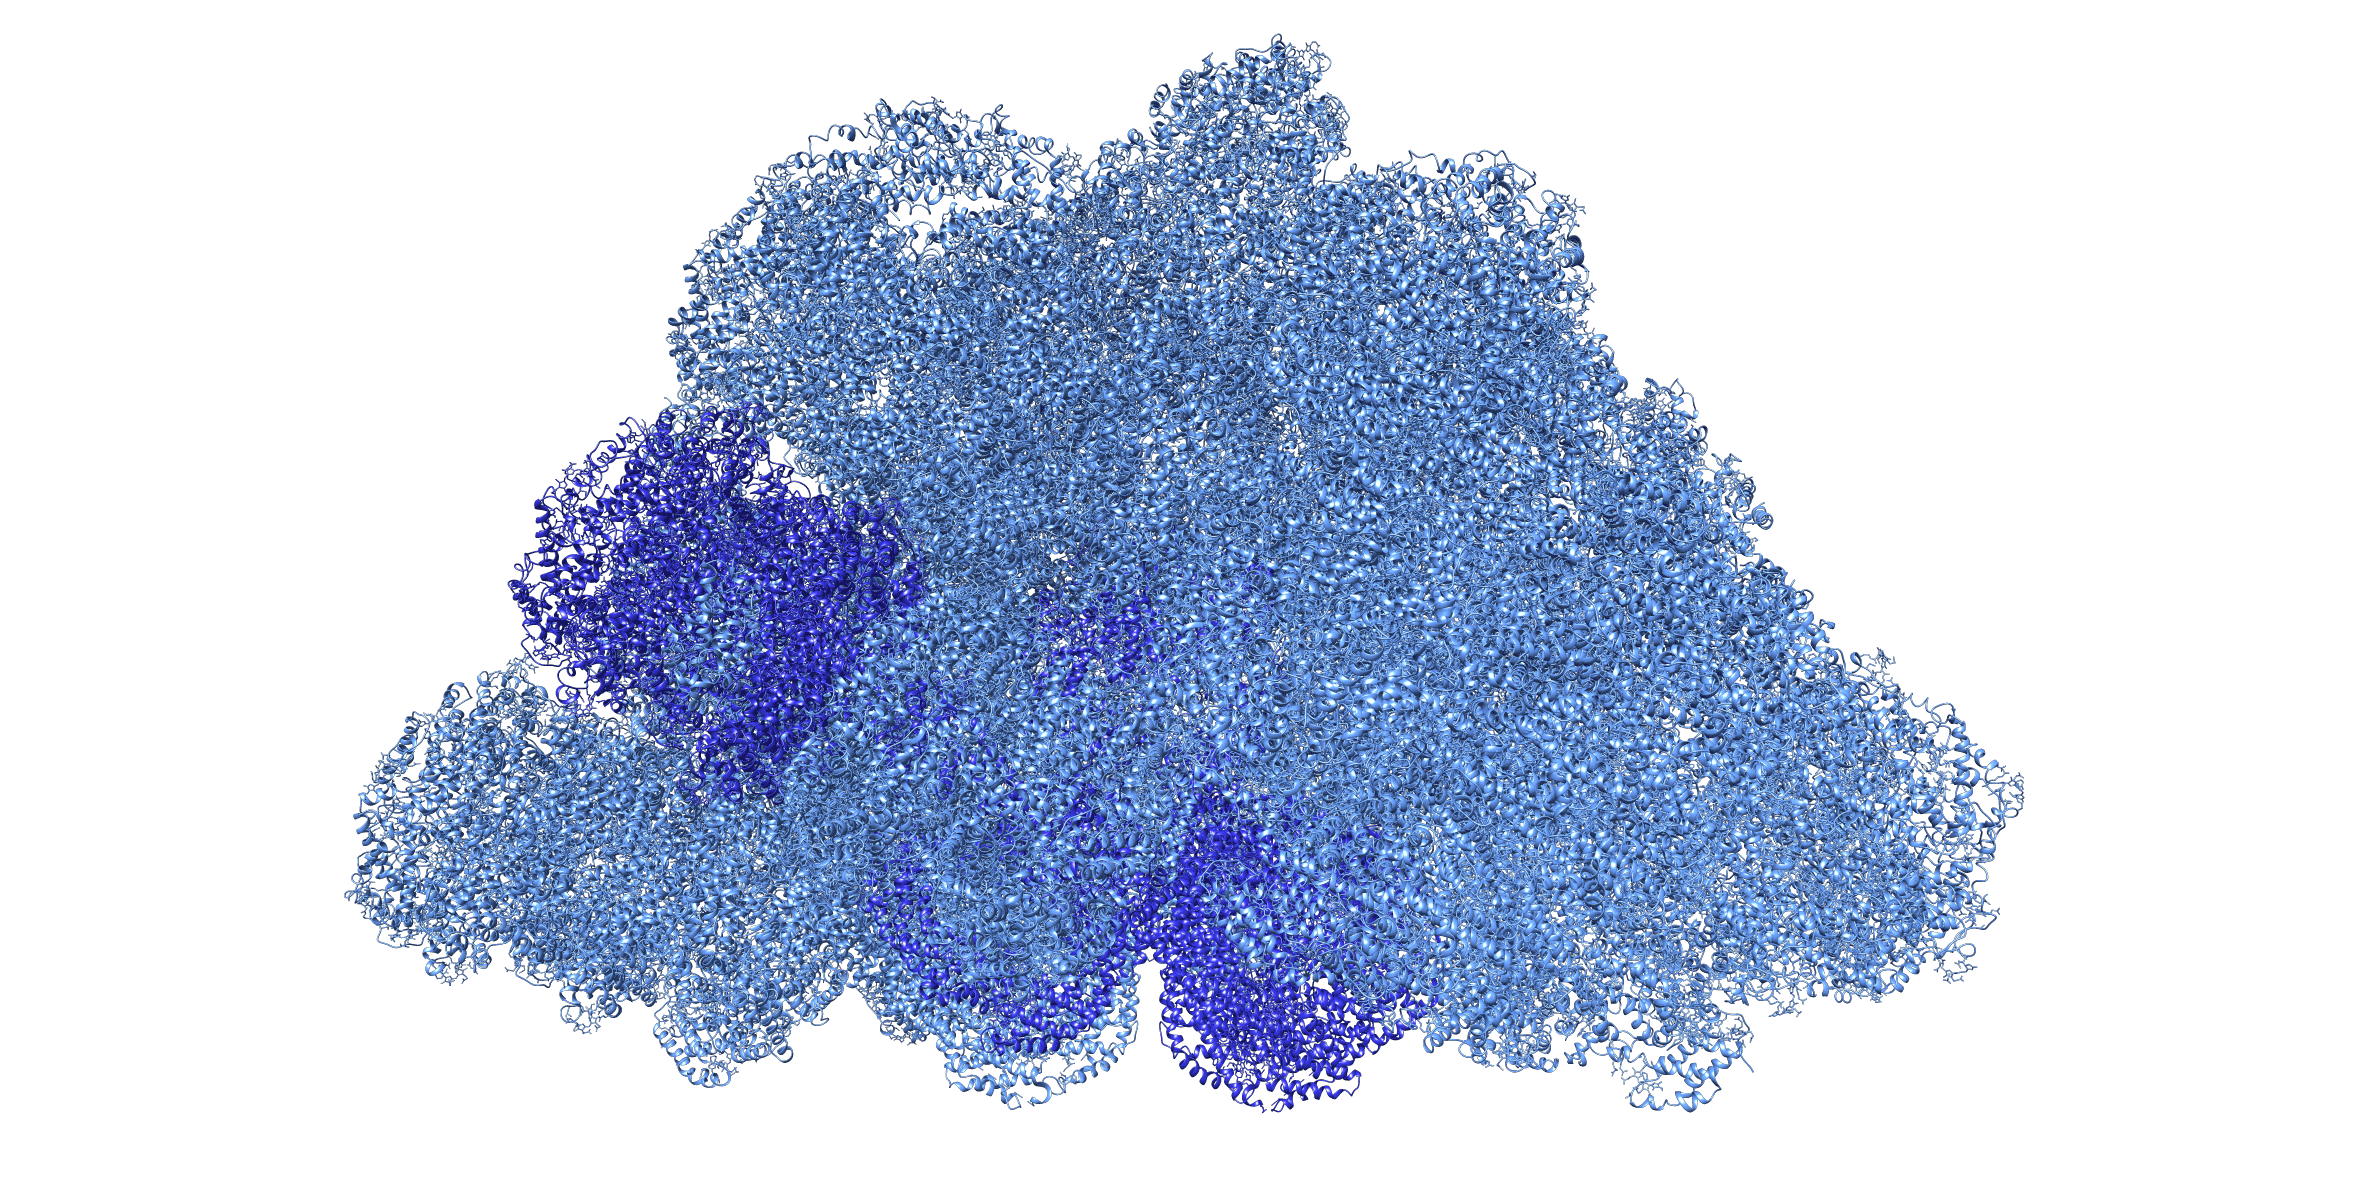
\includegraphics{img/schematics/4_3_1}

\href{http://rcsb.org/structure/6KGX}{\emph{PDB: 6KGX}}
Light-harvesting photocomplexes can comprise hundreds of individual proteins and reach tens of nanometers in size, as you can see in this complex from a red alga (the machinery is closely related to that found in cyanobacteria) \citep{ma2020}. Physically tethering enzymes that function in the same pathway increases efficiency by allowing enzymes that catalyze subsequent steps to hand off substrates. You will see more examples of this theme in the following pages; metabolic enzymes in the cell often cluster together into relay teams.

\hypertarget{ICM_variety}{%
\subsection*{More: ICM variety}\label{ICM_variety}}
\addcontentsline{toc}{subsection}{More: ICM variety}

In some species, like this \emph{Methyloprofundus sedimenti}, the intracytoplasmic membrane is very extensive and appears to be fully separated from the cell membrane. As you can see, it occupies much of the cytoplasmic space.



\hypertarget{htmlwidget-96858fde8a562e7e86cc}{}

\label{fig:4-3a}\protect\hyperlink{tree}{Methyloprofundus sedimenti} Collected by: \protect\hyperlink{elitza_tocheva}{Elitza Tocheva} Movie DOI: \href{https://doi.org/10.22002/D1.1499}{10.22002/D1.1499}

\hypertarget{photosynthesis-contd.}{%
\section{Photosynthesis (cont'd.)}\label{photosynthesis-contd.}}

Other photosynthetic bacteria have taken the specialization of their light-harvesting membranes a step further, expanding not the entire membrane, but simply the hydrophobic interior. The result is a sort of factory called a chlorosome. These structures consist of up to hundreds of thousands of photocomplexes packed tightly inside a lipid monolayer. The size and shape varies between species, from wide lozenges to the thin, curved rod in this \emph{Chloroflexi} cell. They are often tethered close to the membrane (and thus the light), and may be so abundant as to form a nearly continuous layer around the cell. As with intracytoplasmic membrane, their production is controlled in response to need. Chlorosomes, and other compartments you will see soon, challenge the idea that organelles exist only in eukaryotes.



\hypertarget{htmlwidget-7619f7ce8a7b9123d2dc}{}

\label{fig:4-4}\protect\hyperlink{tree}{Chloroflexi} Collected by: \protect\hyperlink{elitza_tocheva}{Elitza Tocheva} Movie DOI: \href{https://doi.org/10.22002/D1.1492}{10.22002/D1.1492}

\hypertarget{enzyme-regulation}{%
\section{Enzyme Regulation}\label{enzyme-regulation}}

Cells are subject to the vagaries of an environment in which conditions often change. To respond, they must be metabolically agile. The production of enzymes is dialed up and down to meet demand, but they can also be regulated in other ways. Degrading and resynthesizing proteins wastes resources and time. So why not just furlough workers when demand lags and call them back in when things pick up again? Cells across all domains of life have evolved an elegant furlough mechanism: enzyme polymerization. You already saw an example of this in Chapter 3: the metabolic enzyme CTP synthase. Another example is the alcohol-acetaldehyde dehydrogenase (AdhE) enzymes that allow \emph{Clostridium thermocellum} like this one to digest cellulose into ethanol. As you can see, AdhE polymerizes into helical filaments called spirosomes. Polymerization can either inactivate an enzyme (e.g.~by occluding its active site), or activate it (e.g.~by changing its conformation to open an active site). Filaments can also regulate activity by changing their conformation; for AdhE, it is thought that spirosomes torque between a compact, inactive form to a more extended, active form (what you see here) \protect\hyperlink{AdhE_spirosome_structure}{Schematic: AdhE spirosome structure}. Whatever the details, polymerization is a rapid way to mobilize (or demobilize) a large number of enzymes for a metabolic task.

Furloughed workers can also be recruited to other projects. Remember that CTP synthase filaments play a secondary, cytoskeletal role. (And perhaps many, if not all, cytoskeletal elements evolved this way.) AdhE spirosomes seem to have a secondary function in cell adhesion, although the details are not yet clear.



\hypertarget{htmlwidget-6afda54ecdc45e366f23}{}

\label{fig:4-5}\protect\hyperlink{tree}{Clostridium thermocellum} Collected by: \protect\hyperlink{elitza_tocheva}{Elitza Tocheva} Movie DOI: \href{https://doi.org/10.22002/D1.1493}{10.22002/D1.1493}

\hypertarget{AdhE_spirosome_structure}{%
\subsection*{Schematic: AdhE spirosome structure}\label{AdhE_spirosome_structure}}
\addcontentsline{toc}{subsection}{Schematic: AdhE spirosome structure}

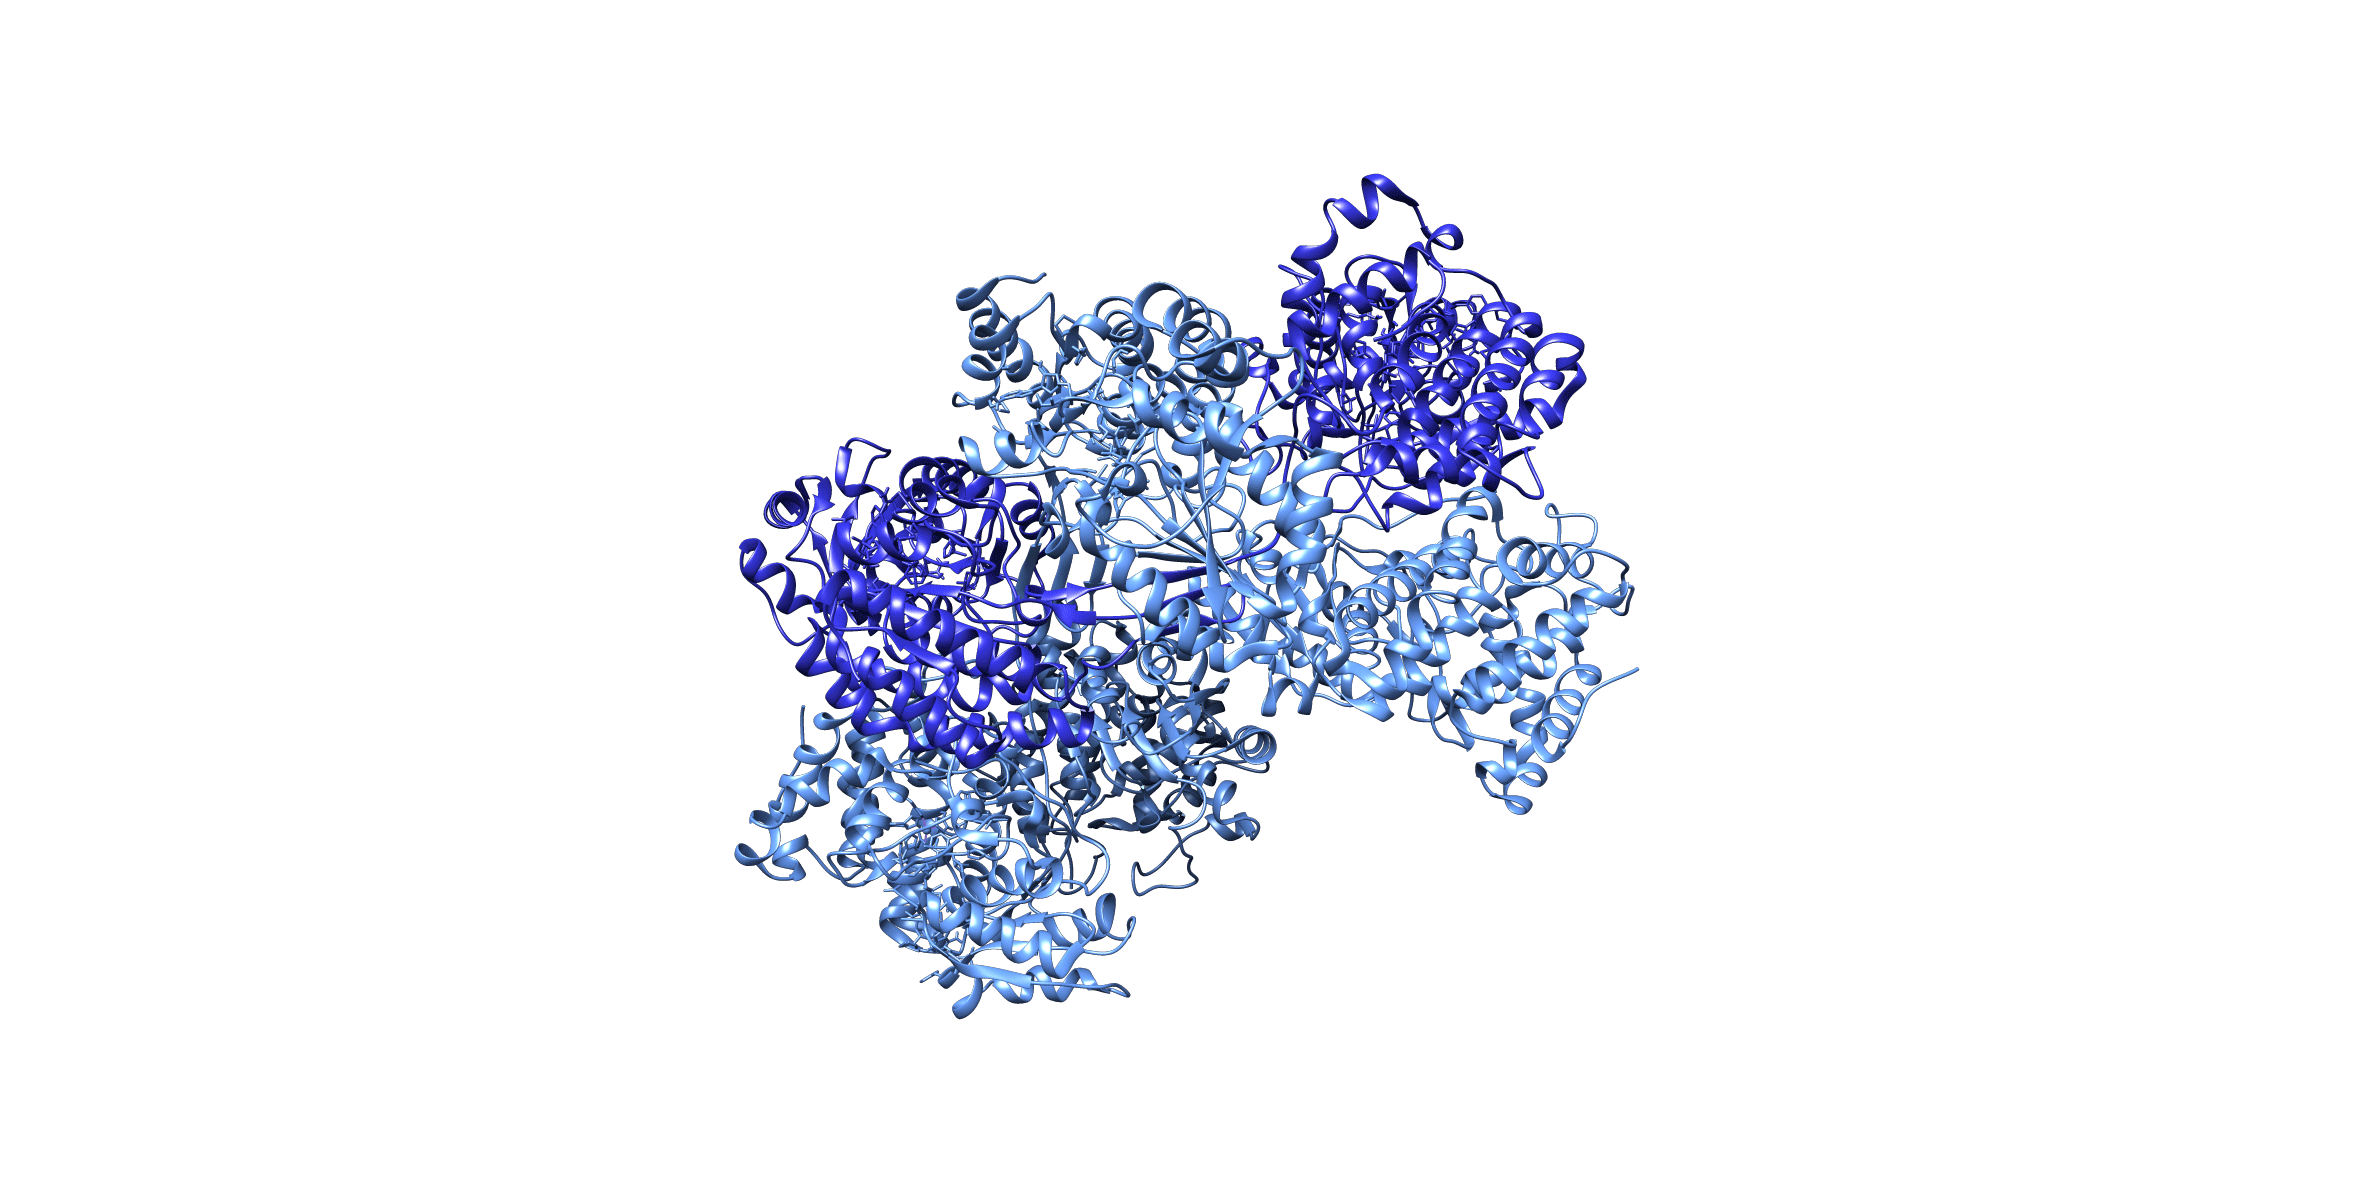
\includegraphics{img/schematics/4_5_1}

\href{http://rcsb.org/structure/6TQH}{\emph{PDB: 6TQH}}
Here you see a short segment of an AdhE spirosome from \emph{Escherichia coli} in the extended, active filament conformation \citep{pony2020}.

\hypertarget{microcompartments}{%
\section{Microcompartments}\label{microcompartments}}

In addition to increasing the number of active workers to boost metabolic output, you could also make them more efficient. One way to do this is by bringing enzymes that work in the same pathway together into an assembly (or disassembly) line. Such factories are common inside cells. You could even go a step further and enclose the factory in a dedicated building. Such structures, found in bacteria but not (as far as we know) archaea, are known as microcompartments--areas of the cytoplasm walled off by a protein shell \protect\hyperlink{Microcompartment_shells}{Schematic: Microcompartment shells}. For instance, \emph{Acetonema longum} like this use a factory called the propanediol utilization, or pdu, microcompartment to increase the efficiency of an enzymatic pathway that breaks down 1,2-propanediol. Illustrating the interlocking lives of microbial communities, 1,2-propanediol is itself the byproduct of the metabolism of other microbes, neighbors in \emph{A. longum}'s environment in the gut of an animal.



\hypertarget{htmlwidget-5e670c875169140aa476}{}

\label{fig:4-6}\protect\hyperlink{tree}{Acetonema longum} Collected by: \protect\hyperlink{elitza_tocheva}{Elitza Tocheva} Movie DOI: \href{https://doi.org/10.22002/D1.1494}{10.22002/D1.1494}

\hypertarget{Microcompartment_shells}{%
\subsection*{Schematic: Microcompartment shells}\label{Microcompartment_shells}}
\addcontentsline{toc}{subsection}{Schematic: Microcompartment shells}

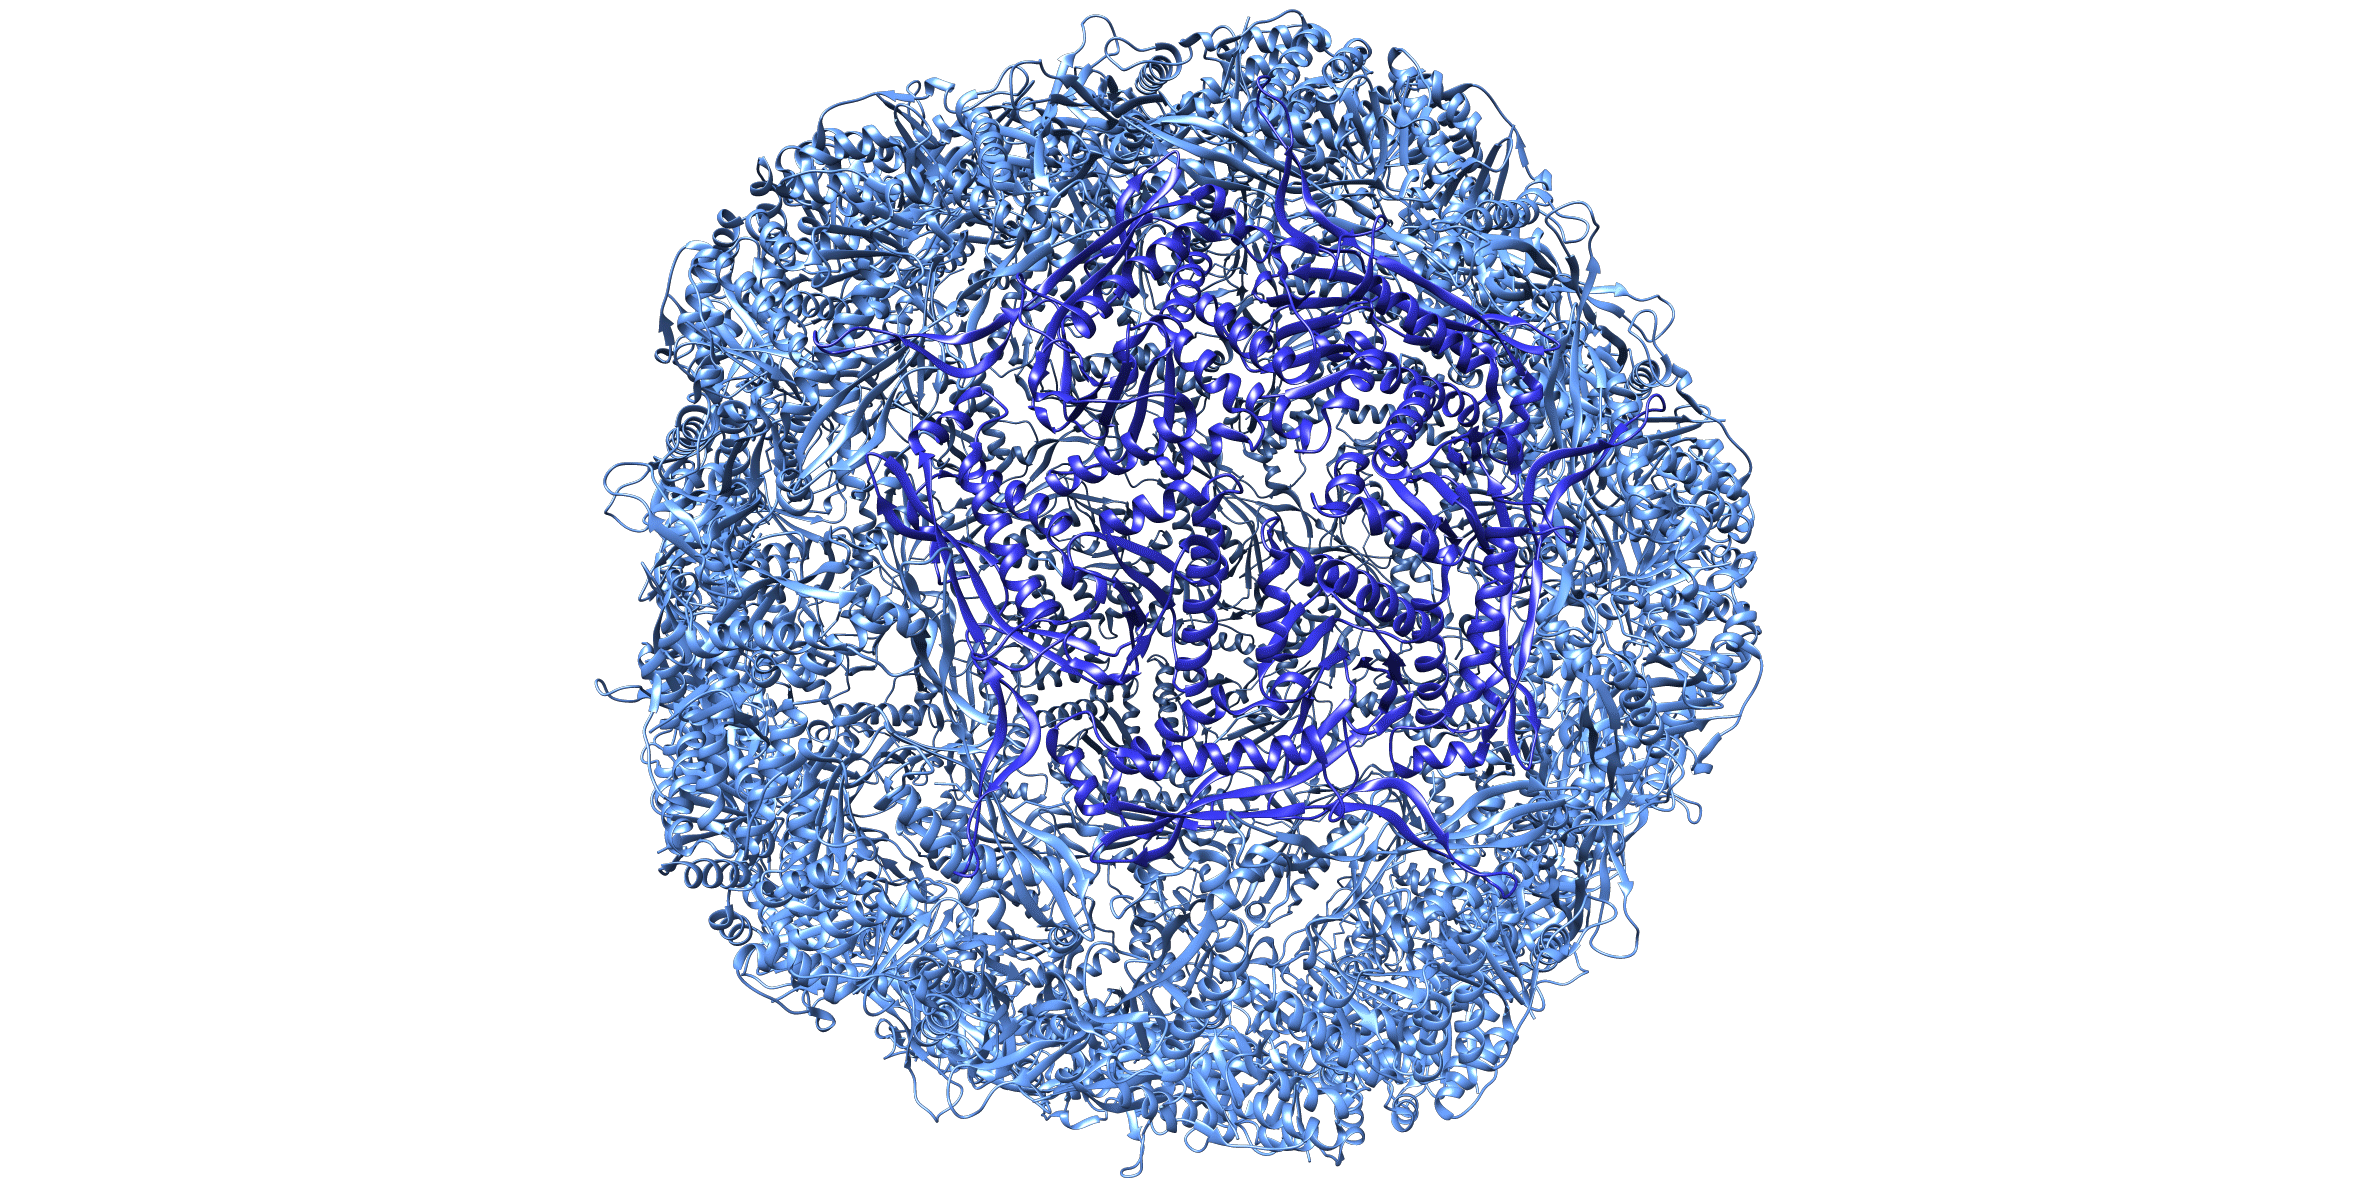
\includegraphics{img/schematics/4_6_1}

\href{http://rcsb.org/structure/3DKT}{\emph{PDB: 3DKT}}
Bacterial microcompartments are typically enclosed by a self-assembling shell formed by just a few proteins. The shell is icosahedral, consisting of hexameric units packed into flat planes, which are joined together by pentamers at the vertices. You can see this arrangement in the shell structure of a microcompartment called an encapsulin that helps \emph{Thermotoga maritima} respond to stress \citep{sutter2008}.

\hypertarget{carboxysomes}{%
\section{Carboxysomes}\label{carboxysomes}}

One of the most impressive bacterial microcompartments is the carboxysome that some species use for carbon fixation (the breakdown of carbon dioxide into usable fuel molecules). Carboxysomes contain tightly packed copies of an enzyme called ribulose bisphosphate carboxylase/oxygenase, or more simply, RuBisCO, which is the most abundant enzyme on Earth. In this case, the shell does more than simply concentrate the enzymes. Oxygen competes with carbon dioxide for binding RuBisCO, so the bacteria include another enzyme in the compartment which converts bicarbonate into CO2, increasing the local concentration and making it readily available to the RuBisCO. The shell may also slow down the diffusion of CO2 out, and O2 in. Carboxysomes were probably unnecessary in early cells because the oxygen level of the environment was much lower. Cells, like this \emph{Thiomonas intermedia}, can contain many carboxysomes. While most are icosahedral, there is significant variation in their forms \protect\hyperlink{Carboxysome_variety}{More: Carboxysome variety}; \protect\hyperlink{Long_carboxysomes}{More: Long carboxysomes}.

In this case, the microcompartment protects its contents from the rest of the cell, but they can also do the reverse. Some metabolic pathways generate toxic intermediates, and bacteria have evolved microcompartments that sequester them so that they do not interfere with other processes in the cell.



\hypertarget{htmlwidget-784a9fb1c4baf87d2669}{}

\label{fig:4-7}\protect\hyperlink{tree}{Thiomonas intermedia} Collected by: \protect\hyperlink{cristina_iancu}{Cristina Iancu} Movie DOI: \href{https://doi.org/10.22002/D1.1495}{10.22002/D1.1495}

\hypertarget{Carboxysome_variety}{%
\subsection*{More: Carboxysome variety}\label{Carboxysome_variety}}
\addcontentsline{toc}{subsection}{More: Carboxysome variety}

Most carboxysomes look like the ones you saw on the last page, but not all. Some are less regular polyhedra, as in this \emph{Halothiobacillus neapolitanus} cell. And some are stranger still \protect\hyperlink{Long_carboxysomes}{More: Long carboxysomes}.



\hypertarget{htmlwidget-fa17d7d85c52ecc4d156}{}

\label{fig:4-7a}\protect\hyperlink{tree}{Halothiobacillus neapolitanus} Collected by: \protect\hyperlink{cristina_iancu}{Cristina Iancu} Movie DOI: \href{https://doi.org/10.22002/D1.1500}{10.22002/D1.1500}

\hypertarget{Long_carboxysomes}{%
\subsection*{More: Long carboxysomes}\label{Long_carboxysomes}}
\addcontentsline{toc}{subsection}{More: Long carboxysomes}

The carboxysomes in this \emph{Hydrogenovibrio crunogenus} have grown abnormally long, extending across the full width of the cell. These are unusual, but less dramatic elongations are common.

This cell also highlights the lability in the outer membrane common in some bacterial species, particularly pathogens. Note how the cell has curled inside its loose outer membrane. You can also see part of it stretching across to another cell in a neighboring hole; they were probably just finishing division when they were pulled apart by sample preparation.



\hypertarget{htmlwidget-27ee8e0ae99dbb1a1a19}{}

\label{fig:4-7b}\protect\hyperlink{tree}{Hydrogenovibrio crunogenus} Collected by: \protect\hyperlink{cristina_iancu}{Cristina Iancu} Movie DOI: \href{https://doi.org/10.22002/D1.1501}{10.22002/D1.1501}

\hypertarget{storage}{%
\section{Storage}\label{storage}}

No matter how efficient your factories are, they need raw materials, and in an ever-changing environment, a cell cannot always depend upon a steady supply chain. How can you help your cell cope with occasional shortages? If you said stockpile, you are in good agreement with Nature. Both bacteria and archaea use storage granules to stockpile essential nutrients. The substrate is usually polymerized for easier packing, like poly-phosphate or the poly-hydroxybutyrate (a carbon store) in these \emph{Cupriavidus necator} granules. No matter what they pack, storage granules are generally spherical, and exhibit a range of sizes \protect\hyperlink{Storage_granule_growth}{More: Storage granule growth}. When the environment is rich in one nutrient but poor in another, cells may stop growing, but keep adding to their cellular stores. You can see that effect in this \emph{C. necator} cell, which has been cultured in a medium with carbon but not enough nitrogen; as a result, it has accumulated very large poly-hydroxybutyrate granules which take up much of the cytoplasmic space.

Storage granules are ubiquitous in bacteria, and you will see them in many of the cells in this book. The most common type is poly-phosphate, which has a characteristic dark appearance in electron microscopy images.



\hypertarget{htmlwidget-58a699e33d3295eda683}{}

\label{fig:4-8}\protect\hyperlink{tree}{Cupriavidus necator} Collected by: \protect\hyperlink{morgan_beeby}{Morgan Beeby} Movie DOI: \href{https://doi.org/10.22002/D1.1496}{10.22002/D1.1496}

\hypertarget{Storage_granule_growth}{%
\subsection*{More: Storage granule growth}\label{Storage_granule_growth}}
\addcontentsline{toc}{subsection}{More: Storage granule growth}

Storage granules expand and contract to accommodate their contents. This \emph{Lysobacter antibioticus} cell exhibits a typical range of sizes of poly-phosphate granules.



\hypertarget{htmlwidget-813ea4f4e68b73112c82}{}

\label{fig:4-8a}\protect\hyperlink{tree}{Lysobacter antibioticus} Collected by: \protect\hyperlink{morgan_beeby}{Morgan Beeby} Movie DOI: \href{https://doi.org/10.22002/D1.1502}{10.22002/D1.1502}

\hypertarget{storage-contd.}{%
\section{Storage (cont'd.)}\label{storage-contd.}}

Some types of storage granules, like poly-phosphate and poly-hydroxybutyrate, are very densely packed and clearly delineated from the rest of the cytoplasm. Others are less tightly packed and more amorphous, like the ones in this \emph{Agrobacterium tumefaciens} cell. We do not yet know what these contain.

In some species, like the \emph{Cupriavidus necator} on the last page, storage granules seem to be positioned randomly in the cell. Other species have more regulated arrangements. \emph{A. tumefaciens} cells always have one poly-phosphate storage granule located near the cell pole. Other species have one at each end of the cell. As we will discuss in Chapter 5, this arrangement can help mother cells deliver a storage granule to each of their daughters during division.

You might expect a close relationship between cellular factories and storage depots. In fact, there does seem to be a relationship between carboxysomes and storage granules, although the details remain unclear \protect\hyperlink{Granule-containing_carboxysomes}{More: Granule-containing carboxysomes}; \protect\hyperlink{Carboxysome-granule_connections}{More: Carboxysome-granule connections}.



\hypertarget{htmlwidget-dc94a18a3d1362e2f3cf}{}

\label{fig:4-9}\protect\hyperlink{tree}{Agrobacterium tumefaciens} Collected by: \protect\hyperlink{elitza_tocheva}{Elitza Tocheva} Movie DOI: \href{https://doi.org/10.22002/D1.1497}{10.22002/D1.1497}

\hypertarget{Granule-containing_carboxysomes}{%
\subsection*{More: Granule-containing carboxysomes}\label{Granule-containing_carboxysomes}}
\addcontentsline{toc}{subsection}{More: Granule-containing carboxysomes}

Small poly-phosphate storage granules are sometimes seen \emph{inside} carboxysomes, as in this \emph{Hydrogenovibrio crunogenus} cell. Their purpose is unknown.



\hypertarget{htmlwidget-e9a7cc297f73475e97a3}{}

\label{fig:4-9a}\protect\hyperlink{tree}{Hydrogenovibrio crunogenus} Collected by: \protect\hyperlink{cristina_iancu}{Cristina Iancu} Movie DOI: \href{https://doi.org/10.22002/D1.1503}{10.22002/D1.1503}

\hypertarget{Carboxysome-granule_connections}{%
\subsection*{More: Carboxysome-granule connections}\label{Carboxysome-granule_connections}}
\addcontentsline{toc}{subsection}{More: Carboxysome-granule connections}

We sometimes see comb-like structures connecting external poly-phosphate storage granules with carboxysomes, as in this \emph{Halothiobacillus neapolitanus} cell. The nature of the relationship between the structures, and the identity and function of the combs, remains a mystery.



\hypertarget{htmlwidget-6eba87fe24c2675a7058}{}

\label{fig:4-9b}\protect\hyperlink{tree}{Halothiobacillus neapolitanus} Collected by: \protect\hyperlink{cristina_iancu}{Cristina Iancu} Movie DOI: \href{https://doi.org/10.22002/D1.1504}{10.22002/D1.1504}

\hypertarget{archaeal-storage-granules}{%
\section{Archaeal Storage Granules}\label{archaeal-storage-granules}}

Archaea also use storage granules, and you will see many examples throughout the book. Compared to the typically-smooth edges of bacterial granules, the edges of many archaeal granules are spikier, giving them a rougher appearance, as in this \emph{Halorubrum litoreum} cell. Others are smooth and, just like in bacteria, they exhibit a range of morphologies depending on what they store. For instance, compare \protect\hyperlink{Haloferax_gibbonsii_granules}{More: Haloferax gibbonsii granules} and \protect\hyperlink{Halohasta_litchfieldiae_granules}{More: Halohasta litchfieldiae granules}.



\hypertarget{htmlwidget-f96b75382fd53a488124}{}

\label{fig:4-10}\protect\hyperlink{tree}{Halorubrum litoreum} Collected by: \protect\hyperlink{ariane_briegel}{Ariane Briegel} Movie DOI: \href{https://doi.org/10.22002/D1.1498}{10.22002/D1.1498}

\hypertarget{Haloferax_gibbonsii_granules}{%
\subsection*{More: Haloferax gibbonsii granules}\label{Haloferax_gibbonsii_granules}}
\addcontentsline{toc}{subsection}{More: Haloferax gibbonsii granules}

Some archaeal cells, like this \emph{Haloferax gibbonsii}, contain many small granules. We do not yet know what they store, but it may be a carbon source.



\hypertarget{htmlwidget-106d9461cf3649b248b6}{}

\label{fig:4-10a}\protect\hyperlink{tree}{Haloferax gibbonsii} Collected by: \protect\hyperlink{ariane_briegel}{Ariane Briegel} Movie DOI: \href{https://doi.org/10.22002/D1.1505}{10.22002/D1.1505}

\hypertarget{Halohasta_litchfieldiae_granules}{%
\subsection*{More: Halohasta litchfieldiae granules}\label{Halohasta_litchfieldiae_granules}}
\addcontentsline{toc}{subsection}{More: Halohasta litchfieldiae granules}

This \emph{Halohasta litchfieldiae} cell has more unusual granules. The high electron-density (darkness) of these punctate structures suggests that they contain metal.



\hypertarget{htmlwidget-9b258df8e1562e59fc7e}{}

\label{fig:4-10b}\protect\hyperlink{tree}{Halohasta litchfieldiae} Collected by: \protect\hyperlink{zhuo_li}{Zhuo Li} Movie DOI: \href{https://doi.org/10.22002/D1.1506}{10.22002/D1.1506}

\hypertarget{further-reading-3}{%
\section{Further Reading}\label{further-reading-3}}

Barry and Gitai (2011). \emph{Self-assembling enzymes and the origins of the cytoskeleton} \citep{barry2011}.

Hoppert and Mayer (1999). \emph{Principles of macromolecular organization and cell function in bacteria and archaea} \citep{hoppert1999}.

Kerfeld et al. (2018). \emph{Bacterial microcompartments} \citep{kerfeld2018}.

Oostergetel et al. (2010). \emph{The chlorosome: A prototype for efficient light harvesting in photosynthesis} \citep{oostergetel2010}.

\hypertarget{division}{%
\chapter{Division}\label{division}}

\begin{quote}
``\ldots{}la rêve de la bactérie : produire deux bactéries.'' (\emph{the dream of the bacterium: to generate two bacteria})
- François Jacob \citep{jacob2002a}
\end{quote}

\hypertarget{segregation}{%
\section{Segregation}\label{segregation}}

Growth only gets you so far. For a coccoid cell, growth increases volume more rapidly than surface area, which is a problem if the cell relies on nutrients imported from the environment. Even if a cell is rod-shaped (so its surface area to volume ratio remains relatively constant with growth), increased volume increases diffusion times, making metabolism less efficient. So what can you do to keep your cell thriving?

It may be time to divide. In essence, division simply splits a cell, the ``mother,'' into two ``daughters.'' Each daughter will be roughly half the size of the mother. A fair split, though, particularly of critical components like the genome, requires careful coordination. Think about the things in your cell. Some of them are present in many copies, like the lipids in the membrane(s) and most of the proteins. Others are present in very few copies, like the chromosome(s). Conceptually, we can sort components into two broad categories: high copy-number and low copy-number items. How would you split the high copy-number items? Easy, right? Just split the cell in the middle and each half will have plenty. This is true, for instance, for the ribosomes and carboxysomes you see in this \emph{Thiomonas intermedia} cell.

What about low copy-number components? Look at the poly-phosphate storage granules in the same cell. To ensure each daughter cell gets the same number, they are evenly spaced along the length of the cell, ready for division in the middle.



\hypertarget{htmlwidget-cac97a17befbc158f476}{}

\label{fig:5-1}\protect\hyperlink{tree}{Thiomonas intermedia} Collected by: \protect\hyperlink{cristina_iancu}{Cristina Iancu} Movie DOI: \href{https://doi.org/10.22002/D1.1507}{10.22002/D1.1507}

\hypertarget{chromosome-segregation}{%
\section{Chromosome Segregation}\label{chromosome-segregation}}

The most important low-copy number component in your cell is its genome; without the instructions, nothing gets built. Reflecting its importance, cells have evolved complex mechanisms to coordinate DNA replication and segregation in time as well as space. The details are beyond our scope here, but we can touch on some general structural principles.

If your cell divides by splitting in the middle, what is the easiest way to get one complete genome copy to each daughter? (Assume your cell has a single chromosome like most bacteria and archaea.) Why not just tether each copy of the chromosome to an opposite pole of the cell? Nearly all bacteria, and many archaea, have a protein called ParB (for Partitioning) that recognizes a specific sequence (ParS) on the chromosome, creating a molecular handle. In \emph{Caulobacter crescentus} like this, ParB also binds a scaffolding protein at the pole called PopZ, hooking the handle to the pole. The PopZ scaffold is not highly ordered, so we see it as a diffuse blob of DNA and protein, noticeable because it excludes other large protein complexes like ribosomes. Several species of bacteria use PopZ or other hub-organizing proteins to tether a genome copy, as well as other things like chemosensory machinery, to the cell pole. Other species use a different mechanism involving many copies of a dynamic protein called ParA that bind and release ParB, ratcheting the ParS handle of the chromosome across the cell. Other components, like the storage granules you just saw, piggyback on this machinery for segregation.

Remember that your cell's chromosome is colossal, so getting the ParS handle to one side is only part of the battle. An army of other proteins work to condense the chromosome to a more manageable volume and wrangle with the division machinery to make sure no straggling loops get caught off-sides.



\hypertarget{htmlwidget-fc4588be5f7944e257d2}{}

\label{fig:5-2}\protect\hyperlink{tree}{Caulobacter crescentus} Collected by: \protect\hyperlink{ariane_briegel}{Ariane Briegel} Movie DOI: \href{https://doi.org/10.22002/D1.1508}{10.22002/D1.1508}

\hypertarget{budding}{%
\section{Budding}\label{budding}}

What if your cell divides a different way? Some bacteria divide not by fission, but by budding, like this \emph{Hyphomonas neptunium} cell. These cells concentrate their growth at the end of a stalk \protect\hyperlink{Hyphomonas_stalk}{More: Hyphomonas stalk}, producing a daughter cell like blowing a bubble. When the bud becomes big enough, they divide at the end of the stalk to release it \protect\hyperlink{Hyphomonas_lifecycle}{More: Hyphomonas lifecycle}. First, though, they have to make sure all the necessary components make it into the bud. The process is most dramatic for the genome; here you can see a copy being transferred through the stalk. The chromosome here resembles a double-stranded DNA helix, but it is actually a higher-order structure of supercoiled DNA. (The crossbands are proteins that help pack the DNA, not hydrogen-bonded bases.)

Several other bacterial species divide by budding, although not all have stalks. Some simply bud from the main cell body; you will see an example later in this chapter.



\hypertarget{htmlwidget-3687d73d6807b6ed73f3}{}

\label{fig:5-3}\protect\hyperlink{tree}{Hyphomonas neptunium} Collected by: \protect\hyperlink{jian_shi}{Jian Shi} Movie DOI: \href{https://doi.org/10.22002/D1.1509}{10.22002/D1.1509}

\hypertarget{Hyphomonas_stalk}{%
\subsection*{More: Hyphomonas stalk}\label{Hyphomonas_stalk}}
\addcontentsline{toc}{subsection}{More: Hyphomonas stalk}

\emph{Hyphomonas neptunium} grow a single stalk from one end of their cell body, similar to the \emph{Caulobacter crescentus} you saw in Chapter 3. The function of the stalk, though, is different in this budding bacterium than in \emph{C. crescentus}, which divide by more conventional fission.



\hypertarget{htmlwidget-8972a2e084bf67f4e8ac}{}

\label{fig:5-3a}\protect\hyperlink{tree}{Hyphomonas neptunium} Collected by: \protect\hyperlink{jian_shi}{Jian Shi} Movie DOI: \href{https://doi.org/10.22002/D1.1519}{10.22002/D1.1519}

\hypertarget{Hyphomonas_lifecycle}{%
\subsection*{More: Hyphomonas lifecycle}\label{Hyphomonas_lifecycle}}
\addcontentsline{toc}{subsection}{More: Hyphomonas lifecycle}

\emph{Hyphomonas neptunium} have evolved a program of stages they pass through in the course of their life. When a newborn cell like this one is released, it is in the ``swarmer'' stage, using its flagellum (discussed in the next chapter) to swim away to a new location. After a while, it settles down, jettisoning its flagellum and growing a stalk with which to make its own bud--the next generation. Once a cell settles down into the stalked stage, it spends the rest of its life sending off buds as long as conditions are good. Only newborn cells are equipped with flagella to go adventuring. We will discuss more lifecycles in Chapter 8.



\hypertarget{htmlwidget-41c34c731a45c63e7277}{}

\label{fig:5-3b}\protect\hyperlink{tree}{Hyphomonas neptunium} Collected by: \protect\hyperlink{jian_shi}{Jian Shi} Movie DOI: \href{https://doi.org/10.22002/D1.1520}{10.22002/D1.1520}

\hypertarget{monoderm-cytokinesis}{%
\section{Monoderm Cytokinesis}\label{monoderm-cytokinesis}}

Once your cell has gotten everything where it needs to go, how can it actually divide? Just as fences separate neighbors, why not use the cell wall to build a septum (``fence'') between the two daughters? That's what this \emph{Staphylococcus aureus} cell is doing, using its cell wall to begin cytokinesis--the physical division of the cytoplasm. In monoderm bacteria like this, with a thick cell wall, the septum is easy to see.



\hypertarget{htmlwidget-da3bd78c198bd3cb956e}{}

\label{fig:5-4}\protect\hyperlink{tree}{Staphylococcus aureus} Collected by: \protect\hyperlink{georges_chreifi}{Georges Chreifi} Movie DOI: \href{https://doi.org/10.22002/D1.1510}{10.22002/D1.1510}

\hypertarget{monoderm-cytokinesis-contd.}{%
\section{Monoderm Cytokinesis (cont'd.)}\label{monoderm-cytokinesis-contd.}}

The division septum grows in from the periphery of the dividing cell toward the middle, drawing the membrane with it. When it reaches the middle, the membrane seals off on each side and the septum separates to release the two cells. The bottom \emph{Tetrasphaera remsis} cell here is at a fairly late stage of this process. This cell also illustrates another point about division: the division plane is not always in the exact middle of the cell. Depending on the species, division may produce daughter cells of unequal sizes.

There can also be more than two daughter cells. Some species undergo simultaneous divisions, with two or more septa forming more or less at the same time. The genus of \emph{Tetrasphaera remsis} gets its name from this property--cells can either divide into two (as in this case) or four roughly spherical cells.



\hypertarget{htmlwidget-087233b7dfef93cf4f69}{}

\label{fig:5-5}\protect\hyperlink{tree}{Tetrasphaera remsis} Collected by: \protect\hyperlink{ariane_briegel}{Ariane Briegel} Movie DOI: \href{https://doi.org/10.22002/D1.1511}{10.22002/D1.1511}

\hypertarget{diderm-cytokinesis}{%
\section{Diderm Cytokinesis}\label{diderm-cytokinesis}}

The cytokinesis process is similar for diderm bacteria, as you can see in this \emph{Idiomarina loihiensis} cell, with the cell wall and inner membrane growing inward. The process is almost complete here, with just a thin channel of cytoplasm in the very middle connecting the daughter cells. Notice the cell wall zippering apart at the edges of the septum. For another example slightly earlier in the process, check out \protect\hyperlink{Sphingopyxis_alaskensis_division}{More: Sphingopyxis alaskensis division}. For a later example, check out \protect\hyperlink{Chloroflexi_division}{More: Chloroflexi division}.



\hypertarget{htmlwidget-46f0e4e3cf0b99a06899}{}

\label{fig:5-6}\protect\hyperlink{tree}{Idiomarina loihiensis} Collected by: \protect\hyperlink{morgan_beeby}{Morgan Beeby} Movie DOI: \href{https://doi.org/10.22002/D1.1512}{10.22002/D1.1512}

\hypertarget{Sphingopyxis_alaskensis_division}{%
\subsection*{More: Sphingopyxis alaskensis division}\label{Sphingopyxis_alaskensis_division}}
\addcontentsline{toc}{subsection}{More: Sphingopyxis alaskensis division}

This diderm cell is about halfway through cytokinesis. The two daughter cells are still connected by a wide bridge of cytoplasm, but the inner membrane and cell wall are drawing in all around.



\hypertarget{htmlwidget-79fadc7ce2aae42d5b1a}{}

\label{fig:5-6a}\protect\hyperlink{tree}{Sphingopyxis alaskensis} Collected by: \protect\hyperlink{morgan_beeby}{Morgan Beeby} Movie DOI: \href{https://doi.org/10.22002/D1.1521}{10.22002/D1.1521}

\hypertarget{Chloroflexi_division}{%
\subsection*{More: Chloroflexi division}\label{Chloroflexi_division}}
\addcontentsline{toc}{subsection}{More: Chloroflexi division}

This diderm cell is in the final stage of cytokinesis. The cytoplasm of the two daughter cells is completely separated by inner membrane and cell wall. The outer membrane, though, has not yet divided.



\hypertarget{htmlwidget-b054d5544acb356ce243}{}

\label{fig:5-6b}\protect\hyperlink{tree}{Chloroflexi} Collected by: \protect\hyperlink{elitza_tocheva}{Elitza Tocheva} Movie DOI: \href{https://doi.org/10.22002/D1.1522}{10.22002/D1.1522}

\hypertarget{diderm-cytokinesis-contd.}{%
\section{Diderm Cytokinesis (cont'd.)}\label{diderm-cytokinesis-contd.}}

In some species, the outer membrane constricts at the same time as the inner membrane, as you saw, for instance, in the \emph{Thiomonas intermedia} cell at the beginning of this chapter. In others, including the cells you saw on the last page, the outer membrane is mainly remodeled at the end of the process, as the cells separate. Other species are intermediate. In \emph{Caulobacter crescentus}, the outer membrane constricts along with the inner membrane and cell wall. At the end of division, though, the inner membrane seals off before the outer membrane, as you can see in this cell, which is at a very late stage of division. For an even later stage, check out \protect\hyperlink{Caulobacter_division}{More: Caulobacter division}.



\hypertarget{htmlwidget-ec86fe3ce91eefb0d0b7}{}

\label{fig:5-7}\protect\hyperlink{tree}{Caulobacter crescentus} Collected by: \protect\hyperlink{zhuo_li}{Zhuo Li} Movie DOI: \href{https://doi.org/10.22002/D1.1513}{10.22002/D1.1513}

\hypertarget{Caulobacter_division}{%
\subsection*{More: Caulobacter division}\label{Caulobacter_division}}
\addcontentsline{toc}{subsection}{More: Caulobacter division}

This \emph{Caulobacter crescentus} cell has completely separated its inner membrane and cell wall, but not yet the outer membrane and surface layer.



\hypertarget{htmlwidget-cb6ba9eb73b57abf3fe5}{}

\label{fig:5-7a}\protect\hyperlink{tree}{Caulobacter crescentus} Collected by: \protect\hyperlink{qing_yao}{Qing Yao} Movie DOI: \href{https://doi.org/10.22002/D1.1523}{10.22002/D1.1523}

\hypertarget{budding-contd.}{%
\section{Budding (cont'd.)}\label{budding-contd.}}

Like monoderms, most diderms divide into roughly equally-sized daughter cells, but not all do. Just like the \emph{Tetrasphaera remsis} you saw earlier, some diderm species produce one larger, and one smaller, daughter, like this \emph{Agrobacterium tumefaciens} cell. In this case, this is because the smaller daughter is technically a bud. \emph{A. tumefaciens} concentrate their growth at one pole, pushing out a bud that, once it becomes large enough, is pinched off and released. The process is very similar to what you saw in \emph{Hyphomonas neptunium}, just without the intervening stalk.



\hypertarget{htmlwidget-bfe01de9947a7292cdd2}{}

\label{fig:5-8}\protect\hyperlink{tree}{Agrobacterium tumefaciens} Collected by: \protect\hyperlink{elitza_tocheva}{Elitza Tocheva} Movie DOI: \href{https://doi.org/10.22002/D1.1514}{10.22002/D1.1514}

\hypertarget{ftsz}{%
\section{FtsZ}\label{ftsz}}

Division can also be asymmetric in a different way: how constricted one side of the cell is relative to the other. You can see that in this \emph{Cupriavidus necator} cell. Asymmetric constriction is most common early in division, but it sometimes persists longer \protect\hyperlink{Asymmetric_constriction}{More: Asymmetric constriction}. To understand how this happens, we need to take a closer look at how cells divide.

To divide, your cell's membrane and cell wall constrict. But remember that the cell wall is resisting the non-trivial force of turgor pressure pushing outward. So how can it overcome this pressure and grow inward? For almost all bacteria and many archaea, the answer is a protein contractor called FtsZ (Filamenting Temperature-Sensitive mutant Z, named for a genetic screen for cells that failed to divide, and therefore grew into long filaments). FtsZ is another piece of your cell's cytoskeleton. Homologous to eukaryotic tubulin, FtsZ polymerizes into filaments that are linked to the cell membrane around the division plane \protect\hyperlink{FtsZ_structure}{Schematic: FtsZ structure}. The filaments are highly dynamic--forming, disassembling and reassembling within seconds.

How does FtsZ find the right spot? There are multiple mechanisms, but an elegant one in cells like this involves an inhibitor that localizes to the cell poles, making a repressive gradient that is strongest at the ends of the cell and weakest in the middle. As the rod-shaped cell grows, the inhibitor concentration at the middle eventually drops low enough that FtsZ can polymerize. Most cells also inhibit FtsZ polymerization when the genome is still in the way, a mechanism called ``nucleoid occlusion.'' Some species do this with an FtsZ-inhibiting protein called MipZ that grabs onto the ParB chromosomal handle, ensuring that FtsZ filaments do not form until the chromosome is clear.

Once everything is ready (the cell is long enough and the nucleoid out of the way), FtsZ filaments form at the division site. Initially, a single, short filament (or a few) appears. Already, this is enough to begin constricting the cell, which explains why many bacterial cells, including this one, start to constrict on one side only. FtsZ filaments run parallel to the cell membrane, so they appear as dots in cross-section; if we rotate the cell around to look down its long axis, we can see them.

\emph{Note: we cannot see the membrane (and any associated FtsZ filaments) all the way around the cell due to the ``missing wedge'' of information in cryoET imaging--see Chapter 1 for an explanation.}



\hypertarget{htmlwidget-dff048c815242ae19dde}{}

\label{fig:5-9}\protect\hyperlink{tree}{Cupriavidus necator} Collected by: \protect\hyperlink{morgan_beeby}{Morgan Beeby} Movie DOI: \href{https://doi.org/10.22002/D1.1515}{10.22002/D1.1515}

\hypertarget{Asymmetric_constriction}{%
\subsection*{More: Asymmetric constriction}\label{Asymmetric_constriction}}
\addcontentsline{toc}{subsection}{More: Asymmetric constriction}

This \emph{C. necator} cell is at a later stage of cytokinesis. In most cells, constriction would be more or less uniform around the circumference by now, but in some cells, including this one, the asymmetry persists.



\hypertarget{htmlwidget-4e7e333974f706339adb}{}

\label{fig:5-9a}\protect\hyperlink{tree}{Cupriavidus necator} Collected by: \protect\hyperlink{morgan_beeby}{Morgan Beeby} Movie DOI: \href{https://doi.org/10.22002/D1.1524}{10.22002/D1.1524}

\hypertarget{FtsZ_structure}{%
\subsection*{Schematic: FtsZ structure}\label{FtsZ_structure}}
\addcontentsline{toc}{subsection}{Schematic: FtsZ structure}

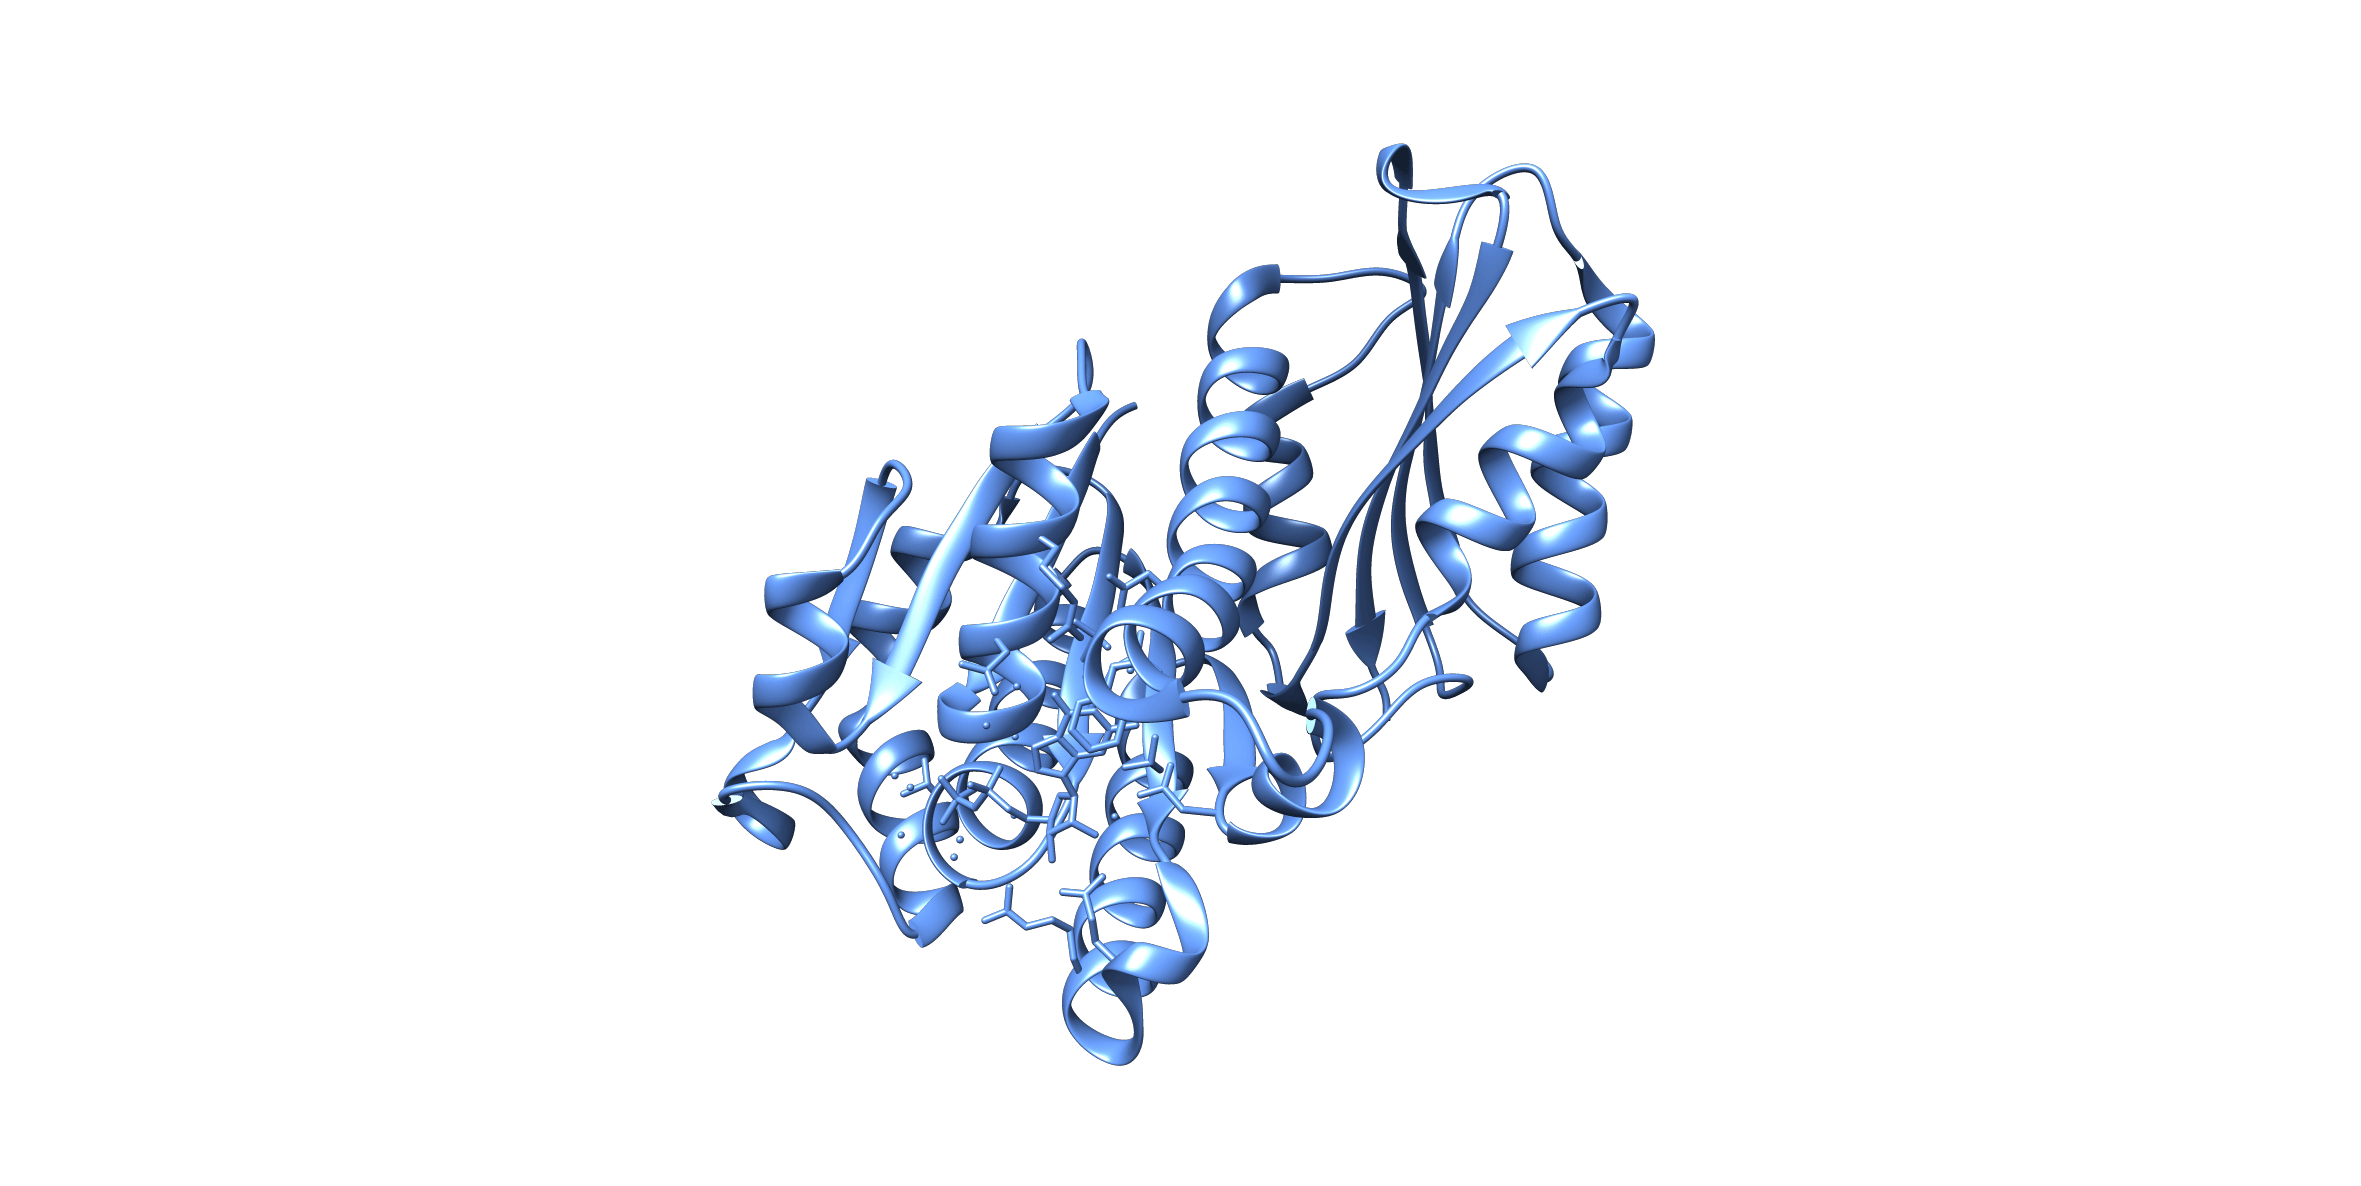
\includegraphics{img/schematics/5_9_1}

\href{http://rcsb.org/structure/5MN4}{\emph{PDB: 5MN4}}
While the structure of FtsZ is known, as seen here from \emph{Staphylococcus aureus} \citep{wagstaff2017}, its mechanism is not. It is an enzyme that hydrolyzes GTP, so one hypothesis is that the curvature of the filament changes as its subunits flip from one conformation to another as a result of the chemical reaction. This different filament conformation may pull inward on the attached membrane, allowing the cell wall to build inward behind it.

\hypertarget{ftsz-contd.}{%
\section{FtsZ (cont'd.)}\label{ftsz-contd.}}

As cytokinesis progresses, FtsZ filaments keep assembling and growing, soon forming a complete ring of long, overlapping filaments around the full circumference of the cell. This drives further constriction more or less uniformly. In this \emph{Caulobacter crescentus} cell in a later stage of division, you can see many FtsZ filaments lined up in cross-section--the dots on both sides of the division plane; if we rotate the cell around, you can see filaments extending on both sides as far as the membrane is visible. (\emph{See the note on the previous page about why we cannot trace the membrane and filaments all the way around.}) They will continue to pull the membrane inward, and direct cell wall to be built behind it, until cytokinesis is complete.



\hypertarget{htmlwidget-d96022d0f7c838e4b950}{}

\label{fig:5-10}\protect\hyperlink{tree}{Caulobacter crescentus} Collected by: \protect\hyperlink{qing_yao}{Qing Yao} Movie DOI: \href{https://doi.org/10.22002/D1.1516}{10.22002/D1.1516}

\hypertarget{escrt}{%
\section{ESCRT}\label{escrt}}

Nearly all bacteria, and many archaea, use FtsZ to divide. Other species of archaea, belonging to the Crenarchaeota phylum, use a different cytoskeletal system called Cdv (for Cell division). Cdv proteins are homologous to proteins of the Endosomal Sorting Complexes Required for Transport (ESCRT). ESCRT proteins were discovered in eukaryotes, where they are involved in many processes that involve cinching off membranes, from the final stage of cell division to virus budding to endocytosis (hence the name), by which cells engulf things from the environment. Again, despite its fundamental importance, we still do not know exactly \emph{how} the ESCRT machinery works to constrict membranes. In archaeal cells like this \emph{Sulfolobus acidocaldarius}, Cdv proteins form a belt of parallel filaments around the middle of the cell, defining the division plane. Notice that the rigid surface layer is dismantled outside the belt so that the membrane can be pulled inward.



\hypertarget{htmlwidget-8d16d41b62fcc035ceea}{}

\label{fig:5-11}\protect\hyperlink{tree}{Sulfolobus acidocaldarius} Collected by: \protect\hyperlink{shrawan_mageswaran}{Shrawan Mageswaran} Movie DOI: \href{https://doi.org/10.22002/D1.1517}{10.22002/D1.1517}

\hypertarget{escrt-contd.}{%
\section{ESCRT (cont'd.)}\label{escrt-contd.}}

The Cdv filaments then pull the membrane inward, constricting the cell, as you can see in this \emph{Sulfolobus acidocaldarius} cell in a later stage of division. Again, the mechanism is unknown, but it may be that the filaments slide against each other into a tightening hourglass-shaped spiral.

The majority of cells divide by one of these two mechanisms--FtsZ or Cdv--but not all do. Some bacterial and archaeal species have neither FtsZ nor Cdv, and we are still figuring out how they divide.



\hypertarget{htmlwidget-23dba7a2c233629aa558}{}

\label{fig:5-12}\protect\hyperlink{tree}{Sulfolobus acidocaldarius} Collected by: \protect\hyperlink{shrawan_mageswaran}{Shrawan Mageswaran} Movie DOI: \href{https://doi.org/10.22002/D1.1518}{10.22002/D1.1518}

\hypertarget{further-reading-4}{%
\section{Further Reading}\label{further-reading-4}}

Badrinarayanan et al. (2015). \emph{Bacterial chromosome organization and segregation} \citep{badrinarayanan2015}.

Hirsch (1974). \emph{Budding bacteria} \citep{hirsch1974}.

Laloux and Jacobs-Wagner (2014). \emph{How do bacteria localize proteins to the cell pole?} \citep{laloux2014}.

Reyes-Lamothe et al. (2012). \emph{Chromosome replication and segregation in bacteria} \citep{reyes-lamothe2012}.

\hypertarget{motility}{%
\chapter{Motility}\label{motility}}

\begin{quote}
``internal combustion engines do no better.''
- Howard Berg \citep{berg1988}
\end{quote}

\hypertarget{flagellum}{%
\section{Flagellum}\label{flagellum}}

Location, location, location. So far, we have focused on how your cell can take the best advantage of its spot in the world. But why not find a better spot? Some cells live stationary lives, attached to a surface or embedded in a biofilm. Many, though, are explorers, using an impressive variety of techniques to move through their environments, finding advantages in places with more food or fewer competitors. In this chapter, we explore how you might make your cell a mobile home.

Most bacteria and archaea live in liquid, so motility means swimming. When you are the size of a cell, though, the backstroke does not get you very far. A rough measure called the Reynolds number describes the relative influence of inertia and viscosity on liquid flow, and this parameter scales with an organism's size. In the low-Reynolds number world of microbes, inertia is virtually nonexistent. When a rod-shaped bacterium stops swimming, it gets to coast only about the diameter of a hydrogen atom (\textasciitilde{}1 Å) before stopping. In this molasses-like environment, rotary propellers work much better than paddles.

Nearly all bacteria that swim use the same propeller: a rotary motor embedded in their envelope that spins a long helical fiber called a flagellum \protect\hyperlink{Flagellum_structure}{Schematic: Flagellum structure}. A universal joint called the hook connects the filament to the motor, translating the rotation. Flagella, like the one on this \emph{Campylobacter jejuni}, are typically many times longer than the cell and take the form of a three-dimensional wave. The filament is highly dynamic, as you would expect, and throughout this book, you will see examples caught in various conformations: straight, curved, or in a typical loose helical waveform like this.



\hypertarget{htmlwidget-7a65905838e7adf0d57a}{}

\label{fig:6-1}\protect\hyperlink{tree}{Campylobacter jejuni} Collected by: \protect\hyperlink{morgan_beeby}{Morgan Beeby} Movie DOI: \href{https://doi.org/10.22002/D1.1525}{10.22002/D1.1525}

\hypertarget{Flagellum_structure}{%
\subsection*{Schematic: Flagellum structure}\label{Flagellum_structure}}
\addcontentsline{toc}{subsection}{Schematic: Flagellum structure}

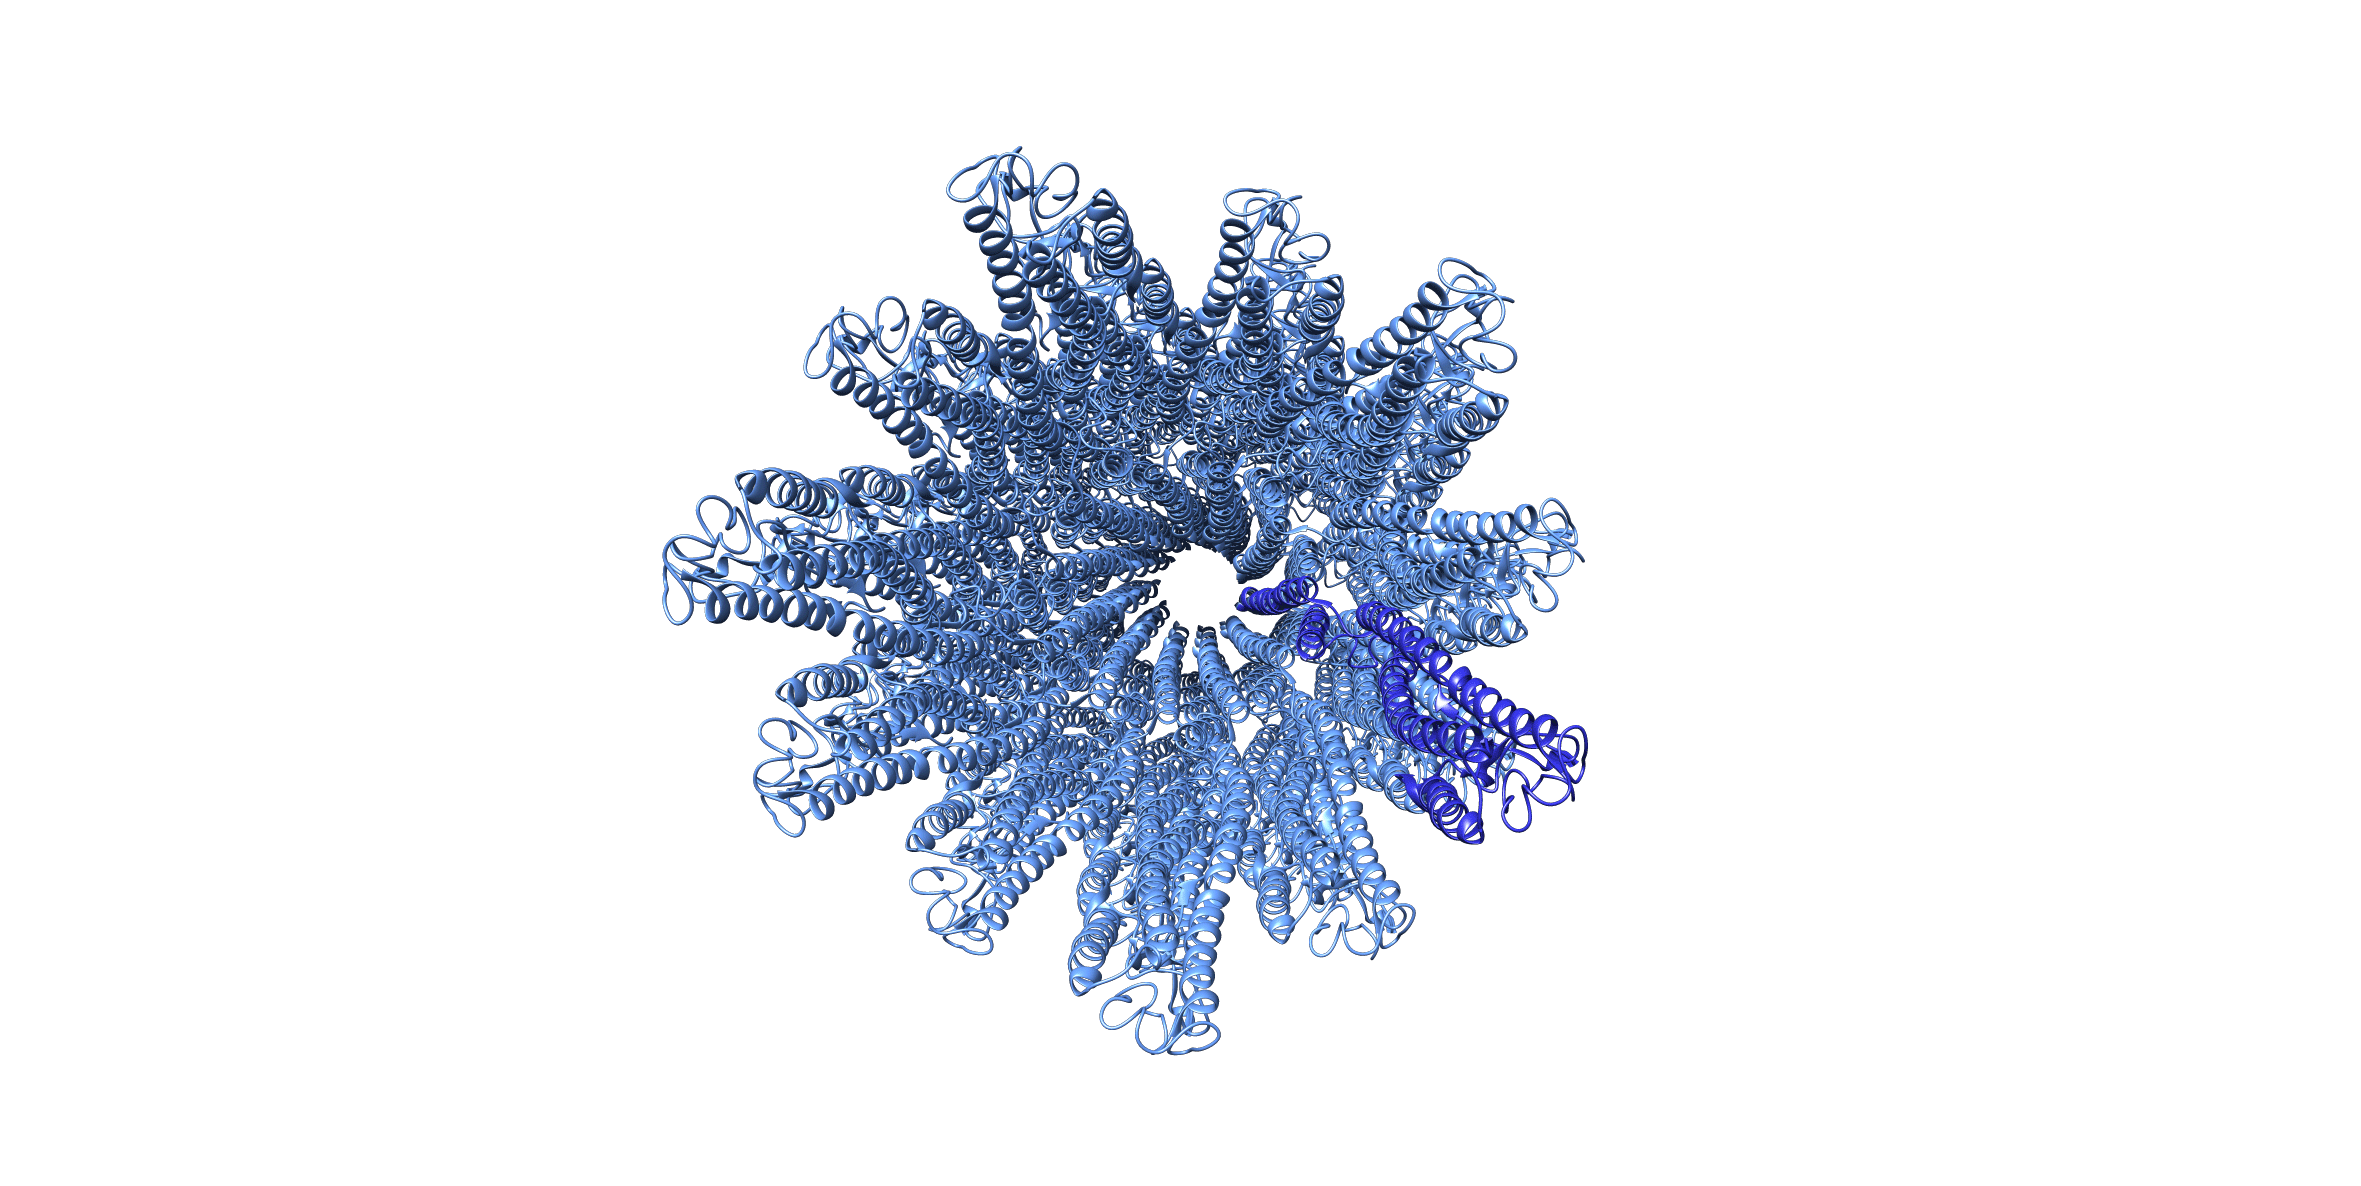
\includegraphics{img/schematics/6_1_1}

\href{http://rcsb.org/structure/5WJT}{\emph{PDB: 5WJT}}
The helical filament of the flagellum is made up of many copies of one or a few flagellin proteins. Each flagellin monomer has a soluble head domain and a hydrophobic alpha-helical tail that bundles together with the tails of other monomers to form a hollow tube. The tube comprises 11 twisting protofilaments, as you can see in this section of a flagellum from \emph{Bacillus subtilis} \citep{wang2017}.

\hypertarget{flagellar-motor}{%
\section{Flagellar Motor}\label{flagellar-motor}}

The motor that spins the flagellum is a complicated molecular machine made of many copies of dozens of different proteins, spanning the cell envelope with components in the cytoplasm, the periplasm (in diderms), and outside the cell, as you can see in this \emph{Bdellovibrio bacteriovorus}. To get a closer look, we can average the individual motors from many cells \protect\hyperlink{Flagellar_motor_structure}{More: Flagellar motor structure}. Broadly, the motor consists of a stationary part (the ``stators'') that anchors the machine in the cell and a rotating part (the ``rotor'') that spins the filament. The torque for spinning the flagellum comes from small movements in the stators that kick the rotor in a circle. The energy for these movements comes from the ion potential across the cell membrane that we discussed in Chapter 2; the stators provide a conduit for protons (in most species) or sodium ions (in some marine species) to diffuse down their chemical gradient into the cytoplasm, powering a conformational change in the stators in the process. The energy demands of the machine are high: a single rotation requires about 1,000 protons to flow through the stators, and the motor may spin at more than 6,000 rotations per minute. The fact that cells pay this energetic cost indicates a strong evolutionary selection for motility, or in other words, the powerful advantage your cell can gain by learning to swim.

While the basic plan of the motor is the same in different species, there are structural differences that reflect the different environments those species encounter \protect\hyperlink{Flagellar_motor_diversity}{Schematic: Flagellar motor diversity}.



\hypertarget{htmlwidget-62709ede1314b7aae67d}{}

\label{fig:6-2}\protect\hyperlink{tree}{Bdellovibrio bacteriovorus} Collected by: \protect\hyperlink{yi-wei_chang}{Yi-Wei Chang} Movie DOI: \href{https://doi.org/10.22002/D1.1526}{10.22002/D1.1526}

\hypertarget{Flagellar_motor_structure}{%
\subsection*{More: Flagellar motor structure}\label{Flagellar_motor_structure}}
\addcontentsline{toc}{subsection}{More: Flagellar motor structure}

This is an average of the flagellar motors from more than one thousand \emph{Bdellovibrio bacteriovorus} cells. Working upward from the base, the major parts of the rotor are the C-ring (for Cytoplasmic), the MS-ring (for Membrane and Supramembrane), the rod, the hook, and finally the filament. They are surrounded by stationary parts: the stator ring (which is dynamic, so we cannot resolve the stators as they cross the inner membrane and connect to the C-ring) and a series of bushings that allow rotation within the cell wall (the Periplasmic or P-ring) and outer membrane (Lipopolysaccharide or L-ring). Additional cytoplasmic components form the export apparatus, which is involved in assembly (discussed on the next page).



\hypertarget{htmlwidget-957400500e65eb36e62e}{}

\label{fig:6-2a}\protect\hyperlink{tree}{Bdellovibrio bacteriovorus} Collected by: \protect\hyperlink{yi-wei_chang}{Yi-Wei Chang} Movie DOI: \href{https://doi.org/10.22002/D1.1537}{10.22002/D1.1537}

\hypertarget{Flagellar_motor_diversity}{%
\subsection*{Schematic: Flagellar motor diversity}\label{Flagellar_motor_diversity}}
\addcontentsline{toc}{subsection}{Schematic: Flagellar motor diversity}

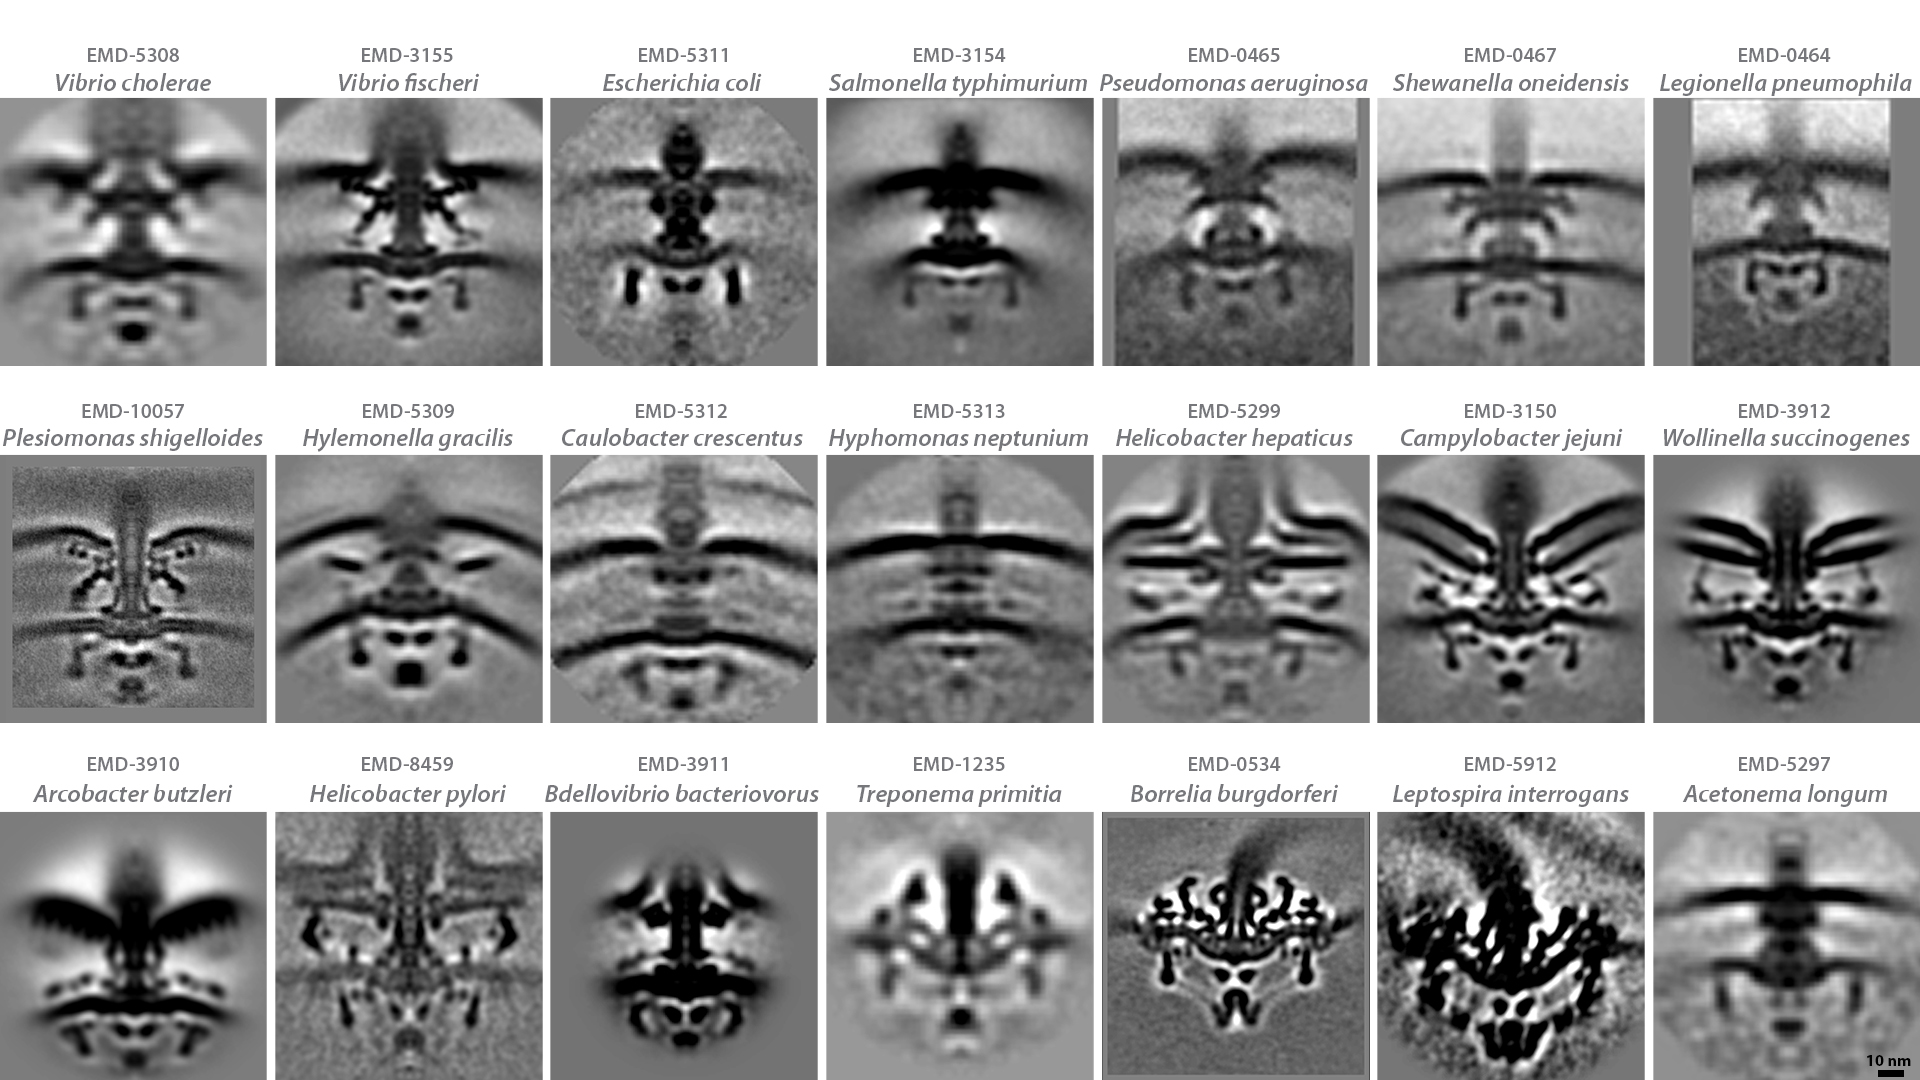
\includegraphics{img/schematics/6_2_1}

As you can see in these averages of flagellar motors from different species \citep{murphy2006} \citep{chen2011} \citep{zhao2014} \citep{beeby2016} \citep{qin2017} \citep{chaban2018} \citep{kaplan2019} \citep{ferreira2019} \citep{chang2019}, bacteria have evolved structural adaptations of their motors to better suit their environments. For instance, if your cell is a pathogen colonizing an animal's intestinal tract (like \emph{Campylobacter jejuni}), it will be swimming in more viscous conditions and may therefore have evolved a wider stator ring to generate more torque, along with reinforced anchors in the cell wall and outer membrane to withstand that added torque.

\hypertarget{flagellar-assembly}{%
\section{Flagellar Assembly}\label{flagellar-assembly}}

Operating the flagellar motor is impressive, but so is building it in the first place. Remember that the envelope of bacterial cells is a complicated multilayered barrier. The flagellar motor has about two dozen unique components, each present in many copies, embedded in every layer of the cell envelope. How can your cell get all hundred or more components (tens of thousands if you count the components of the filament) where they need to go? Making the feat even more impressive, the machine builds itself, assembling from the inside out. First the components associated with the inner membrane come together, forming an ``export apparatus'' which pumps subsequent components across the membrane to assemble in the periplasm and outer membrane (if the cell is a diderm). The energy for this process comes from an ATPase at the base of the machine. You can see a late stage in the assembly process in this \emph{Hylemonella gracilis} cell. The final piece to be assembled (still missing here) is the flagellar filament, which continues the pattern of outward assembly; flagellin monomers travel through the hollow tube to take their places at the tip. Flagellar motors can also disassemble, for instance when the filament is broken \protect\hyperlink{Flagellar_motor_disassembly}{More: Flagellar motor disassembly}, and cells may make many new flagella throughout their lifetime.

So the flagellar motor is not just a machine for motility; it is also a machine to secrete molecules outside the cell. Bacteria and archaea contain many such ``secretion systems,'' each specialized to transport specific macromolecules (e.g.~DNA or a protein toxin) across cell envelopes--both their own and sometimes others. Secretion systems are classified by evolutionary relatedness; there are currently \textasciitilde{}10 types recognized in bacteria, some of which are also present in archaea. The flagellar motor is an example of a Type III Secretion System. You will see another member of this family in Chapter 9, and examples of many other types in the rest of the book, starting in just a few pages.



\hypertarget{htmlwidget-38b415878041db865ccf}{}

\label{fig:6-3}\protect\hyperlink{tree}{Hylemonella gracilis} Collected by: \protect\hyperlink{yi-wei_chang}{Yi-Wei Chang} Movie DOI: \href{https://doi.org/10.22002/D1.1527}{10.22002/D1.1527}

\hypertarget{Flagellar_motor_disassembly}{%
\subsection*{More: Flagellar motor disassembly}\label{Flagellar_motor_disassembly}}
\addcontentsline{toc}{subsection}{More: Flagellar motor disassembly}

When flagella break (or in some species, like \emph{Caulobacter crescentus}, are ejected so the cell can attach to a surface), the motor is disassembled, usually beginning with the export apparatus. Not everything is dismantled, though; the P- and L-rings remain in place in the cell wall and outer membrane, respectively, as you can see in this \emph{Pseudomonas aeruginosa} cell. We do not know if the cell has a reason for leaving them there, but one possibility is that they may function as a plug for the outer membrane when the hook is no longer present.



\hypertarget{htmlwidget-07c6c1ee1a6c1cb5229f}{}

\label{fig:6-3a}\protect\hyperlink{tree}{Pseudomonas aeruginosa} Collected by: \protect\hyperlink{ariane_briegel}{Ariane Briegel} Movie DOI: \href{https://doi.org/10.22002/D1.1538}{10.22002/D1.1538}

\hypertarget{flagella-patterns}{%
\section{Flagella Patterns}\label{flagella-patterns}}

Once assembled, flagella can work in different ways. The motor is bidirectional, and can rotate either clockwise or counterclockwise. Depending on the number and location of flagella on the cell (and the cell's shape), this can push the cell, pull it, or give rise to even more complicated swimming behavior. Some bacterial species, like the \emph{Bdellovibrio bacteriovorus} you just saw, are monotrichous (``single haired''), with one flagellum located at one pole to push/pull the cell. Other species, like the \emph{Campylobacter jejuni} here, have bipolar flagella--one at each end. Still others are lophotrichous (``crest-haired''), with a clump of flagella \protect\hyperlink{Lophotrichous_bacteria}{More: Lophotrichous bacteria}.



\hypertarget{htmlwidget-b5347b983529eaa3a21b}{}

\label{fig:6-4}\protect\hyperlink{tree}{Campylobacter jejuni} Collected by: \protect\hyperlink{morgan_beeby}{Morgan Beeby} Movie DOI: \href{https://doi.org/10.22002/D1.1528}{10.22002/D1.1528}

\hypertarget{Lophotrichous_bacteria}{%
\subsection*{More: Lophotrichous bacteria}\label{Lophotrichous_bacteria}}
\addcontentsline{toc}{subsection}{More: Lophotrichous bacteria}

Many lophotrichous species, like the \emph{Hylemonella gracilis} you saw in Chapter 3--Length or this \emph{Helicobacter pylori}, have a tuft of flagella at their cell pole. In some species, though, the tuft is located elsewhere; for example, a clump of flagella on the concave side of banana-shaped \emph{Selenomonas artemidis} pushes the cells sideways in a seesawing swimming pattern.



\hypertarget{htmlwidget-d840b1fa6d51eba30329}{}

\label{fig:6-4a}\protect\hyperlink{tree}{Helicobacter pylori} Collected by: \protect\hyperlink{yi-wei_chang}{Yi-Wei Chang} Movie DOI: \href{https://doi.org/10.22002/D1.1539}{10.22002/D1.1539}

\hypertarget{flagella-patterns-contd.}{%
\section{Flagella Patterns (cont'd.)}\label{flagella-patterns-contd.}}

Still other species are peritrichous (``hair around''), with multiple flagella distributed randomly around the cell, as you can see on this \emph{Pseudomonas flexibilis}. The number of flagella varies between different species, from relatively few here to considerably more \protect\hyperlink{Proteus_mirabilis_flagella}{More: Proteus mirabilis flagella}. The well-known model system \emph{Escherichia coli} is also peritrichously flagellated. In this arrangement, when the flagellar motors are all rotating one direction (counter-clockwise), the flagella form a whip-like bundle that propels the cell to ``run'' in a straight line. When one or more motors switch to clockwise rotation, the flagella dissociate from the bundle and ``tumble'' the cell to face a new direction. In the next chapter, you will see how cells use this behavior to seek out favorable spots.



\hypertarget{htmlwidget-3eb55f1228b499733aff}{}

\label{fig:6-5}\protect\hyperlink{tree}{Pseudomonas flexibilis} Collected by: \protect\hyperlink{morgan_beeby}{Morgan Beeby} Movie DOI: \href{https://doi.org/10.22002/D1.1529}{10.22002/D1.1529}

\hypertarget{Proteus_mirabilis_flagella}{%
\subsection*{More: Proteus mirabilis flagella}\label{Proteus_mirabilis_flagella}}
\addcontentsline{toc}{subsection}{More: Proteus mirabilis flagella}

\emph{Proteus mirabilis} adapt their motility machinery to their environment. In liquid, the short rod-shaped cells swim with the help of a handful of flagella distributed peritrichously around their cell body. When they encounter a solid surface, the cells elongate and build many more flagella, as you can see on this cell. Instead of swimming, they now use their flagella to propel themselves in groups across the surface, a motility mode known as ``swarming.'' This is an example of a differentiated lifecycle, which will come up again in Chapter 8.



\hypertarget{htmlwidget-f45405f0d421045faac8}{}

\label{fig:6-5a}\protect\hyperlink{tree}{Proteus mirabilis} Collected by: \protect\hyperlink{qing_yao}{Qing Yao} Movie DOI: \href{https://doi.org/10.22002/D1.1540}{10.22002/D1.1540}

\hypertarget{sheathed-flagella}{%
\section{Sheathed Flagella}\label{sheathed-flagella}}

You may have noticed that some of the flagella in this chapter were enclosed within the outer membrane of the cell. We call these ``sheathed'' flagella. It is a common adaptation in pathogenic species, like this \emph{Helicobacter hepaticus}. Flagella offer pathogens a great advantage in colonizing their hosts; hosts in turn have learned to use them to identify potential invaders. As a result, the innate immune response of many eukaryotes, from plants to insects to humans, has evolved to recognize the telltale and abundant signal of flagellin proteins in the long filament. If your cell aims to take up residence in such a host, it could therefore benefit from cloaking this strongly antigenic feature.



\hypertarget{htmlwidget-2f28d0a6a86f0ad1d02d}{}

\label{fig:6-6}\protect\hyperlink{tree}{Helicobacter hepaticus} Collected by: \protect\hyperlink{ariane_briegel}{Ariane Briegel} Movie DOI: \href{https://doi.org/10.22002/D1.1530}{10.22002/D1.1530}

\hypertarget{periplasmic-flagella}{%
\section{Periplasmic Flagella}\label{periplasmic-flagella}}

If your cell \emph{is} a pathogen, swimming can be very useful, but so can burrowing, for instance between cells in host tissue. To do this, why not turn your cell into a corkscrew with the equipment at hand? Some cells do just this, wrapping their flagellum around their body to back out of a tight spot, or burrow into one. Other, diderm species like the \emph{Borrelia burgdorferi} here have turned the temporary adaptation into a permanent one: they assemble their flagella \emph{inside} the cell envelope, with the filaments wrapping around between the cell wall and outer membrane. These ``periplasmic'' flagella are usually multiple, arising from one or both ends of the cell, and pack together into a helical ribbon. The helical ribbon helps give these Spirochetes (``spiral haired'') their characteristic shape; mutants that cannot make flagella are simple rods. Some spirochetes also have additional features that may help them move around in animal hosts \protect\hyperlink{Treponema_primitia}{More: Treponema primitia}



\hypertarget{htmlwidget-dc18cde5c9a80ff9766d}{}

\label{fig:6-7}\protect\hyperlink{tree}{Borrelia burgdorferi} Collected by: \protect\hyperlink{ariane_briegel}{Ariane Briegel} Movie DOI: \href{https://doi.org/10.22002/D1.1531}{10.22002/D1.1531}

\hypertarget{Treponema_primitia}{%
\subsection*{More: Treponema primitia}\label{Treponema_primitia}}
\addcontentsline{toc}{subsection}{More: Treponema primitia}

\emph{Treponema primitia} like this are commensal residents of the termite gut, helping break down cellulose. In addition to two periplasmic flagella, the cells have arrays of bowl- and hook-like structures on their surface, the function of which, likely related to motility, remains mysterious.



\hypertarget{htmlwidget-8f1913eced485239f126}{}

\label{fig:6-7a}\protect\hyperlink{tree}{Treponema primitia} Collected by: \protect\hyperlink{gavin_murphy}{Gavin Murphy} Movie DOI: \href{https://doi.org/10.22002/D1.1541}{10.22002/D1.1541}

\hypertarget{archaellum}{%
\section{Archaellum}\label{archaellum}}

Archaea swim, too. And as you might expect, they use similar machinery to do so: an envelope-embedded motor that spins a long extracellular filament. Despite the structural similarity, the machinery evolved independently, another indication of the strong advantage conferred by swimming. To reflect this similar-but-not-the-same character, we call the archaeal analogue of the bacterial flagellum the archaellum. Unlike the flagellum, which is a Type III Secretion System, the archaellum is a Type II Secretion System. As you can see on this \emph{Methanoregula formicica} cell, archaella are narrower than flagella \protect\hyperlink{Archaellum_structure}{Schematic: Archaellum structure}. The motor is also different, and uses the ATPase at the base not just for assembly, but also to power rotation for swimming. Like flagella, archaellar motors can rotate in either direction, resulting in the filaments pushing or pulling the cell.



\hypertarget{htmlwidget-07d563b5a61b9b66b7a3}{}

\label{fig:6-8}\protect\hyperlink{tree}{Methanoregula formicica} Collected by: \protect\hyperlink{ariane_briegel}{Ariane Briegel} Movie DOI: \href{https://doi.org/10.22002/D1.1532}{10.22002/D1.1532}

\hypertarget{Archaellum_structure}{%
\subsection*{Schematic: Archaellum structure}\label{Archaellum_structure}}
\addcontentsline{toc}{subsection}{Schematic: Archaellum structure}

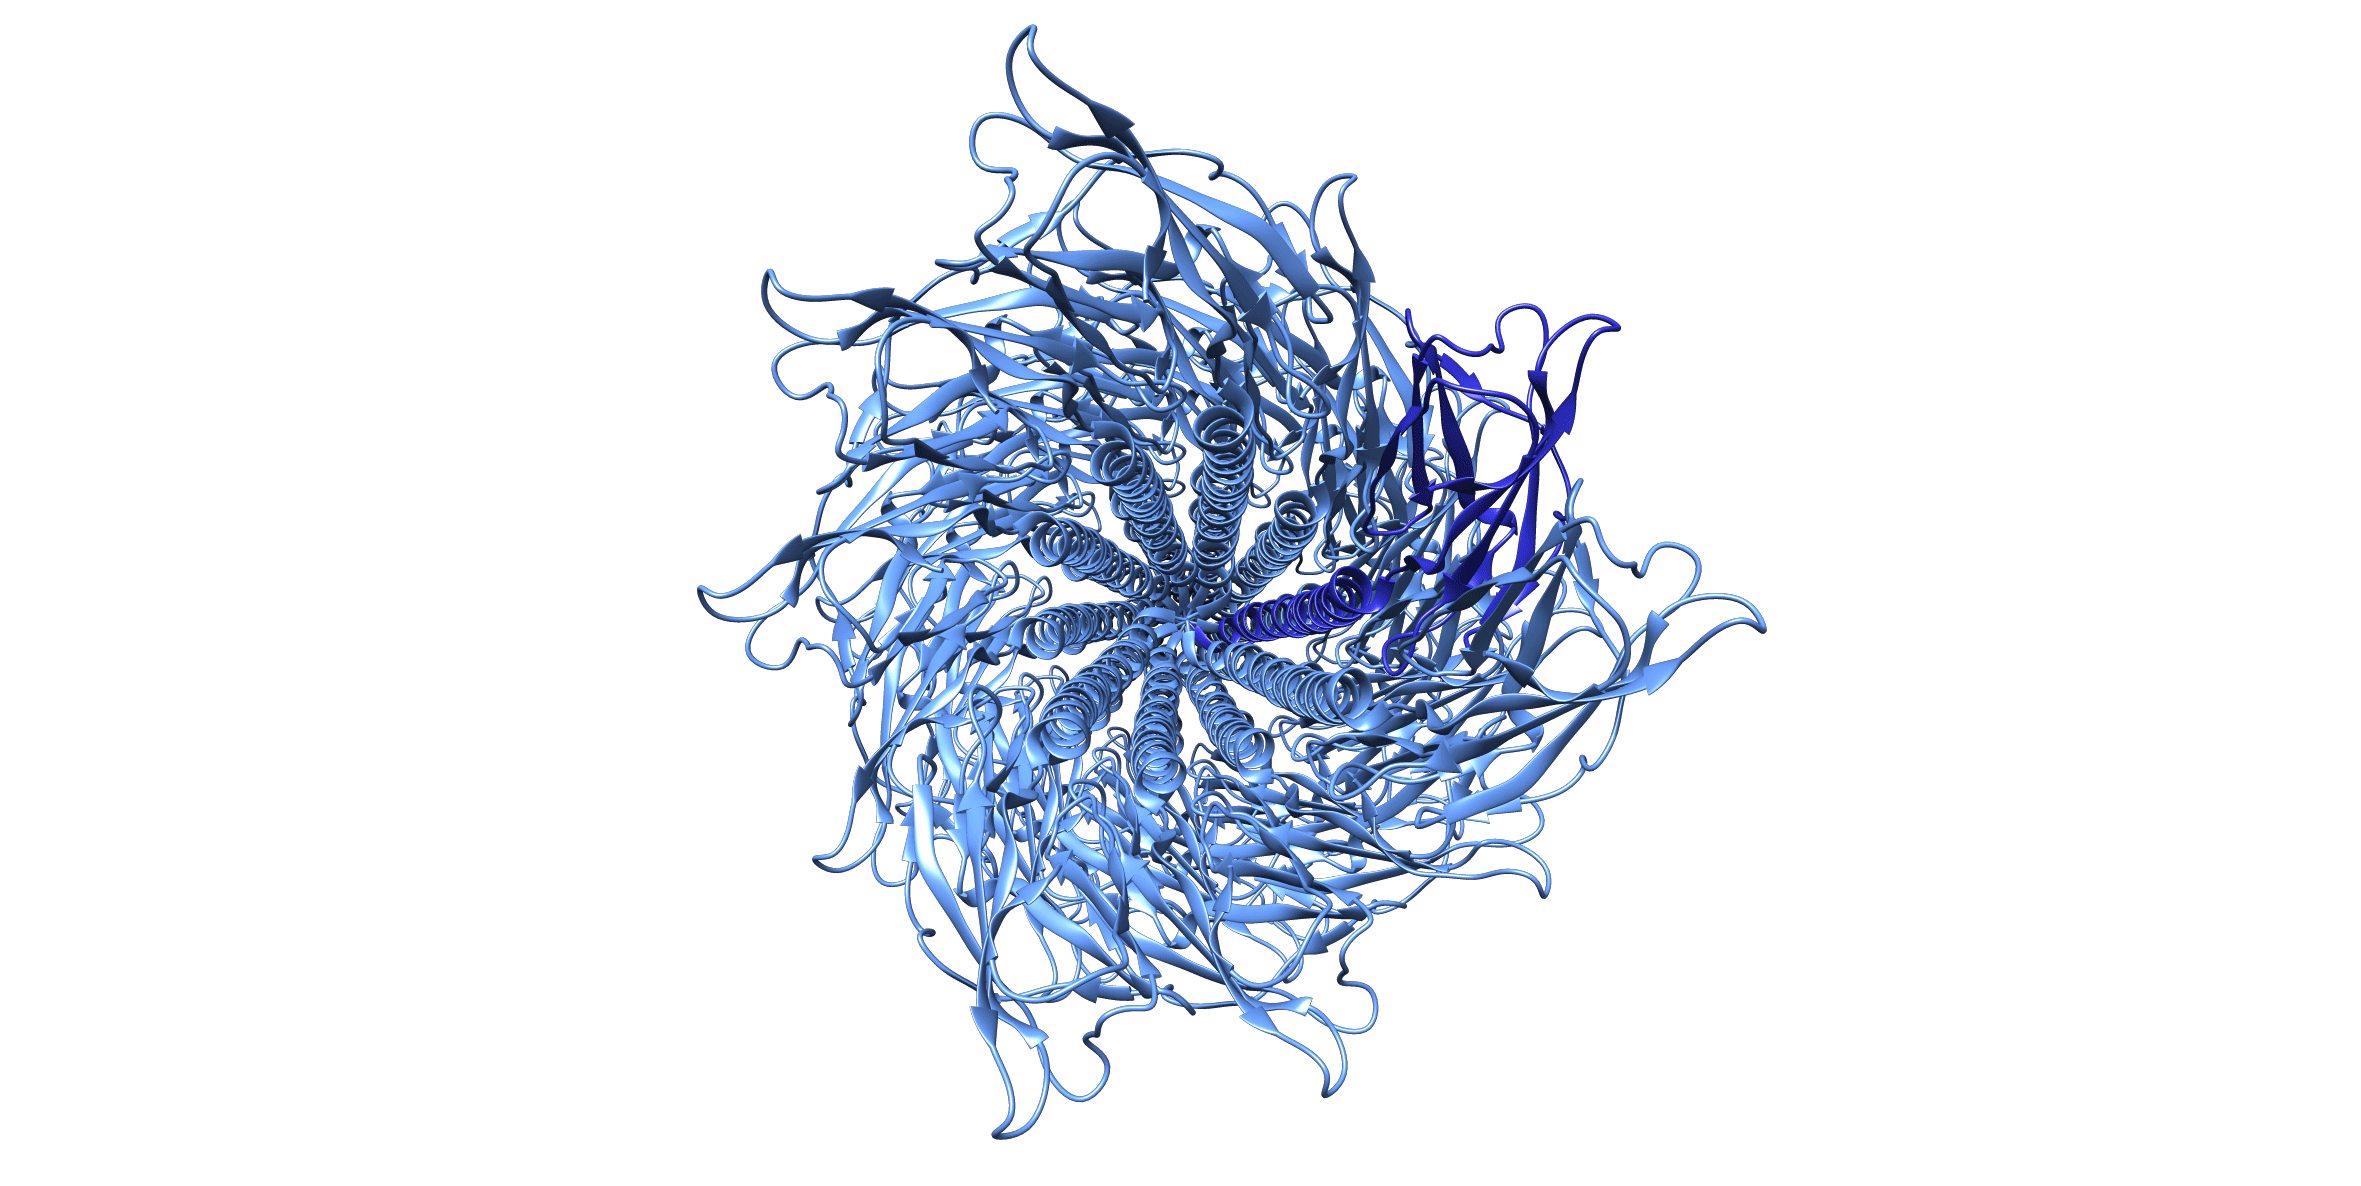
\includegraphics{img/schematics/6_8_1}

\href{http://rcsb.org/structure/5TFY}{\emph{PDB: 5TFY}}
The overall architecture of the helical archaellum is similar to that of the bacterial flagellum, as you can see in this structure from \emph{Methanospirillum hungatei} \citep{poweleit2016}. Each protein subunit is smaller, however, resulting in a narrower filament diameter: \textasciitilde{}10 nm, compared to \textasciitilde{}24 nm for the flagellum. They are also more tightly packed, so there is no central channel. And, unlike flagella, the filament assembles from the base.

\hypertarget{archaella-patterns}{%
\section{Archaella Patterns}\label{archaella-patterns}}

Similar to flagella in bacteria, different archaeal species employ different numbers and patterns of archaella. Some species have one, others have many, either distributed peritrichously (all around) as in the \emph{Methanoregula formicica} you just saw, or lophotrichously (clumped) as in this \emph{Thermococcus kodakaraensis}. In \emph{T. kodakaraensis} and related species, an additional structure--a large conical plate--is seen in the cytoplasm, perhaps providing leverage for the multiple motors. The plate has a unique structure \protect\hyperlink{Cone_structure}{More: Cone structure} and may act as an organizing center akin to the polar PopZ structure we discussed in the last chapter \protect\hyperlink{Organizing_center}{More: Organizing center}. Note the two peaks on this cone; it may be in the process of replicating in preparation for division.

A leveraging plate must not be essential, however, because not all lophotrichous archaea use one \protect\hyperlink{Lophotrichous_Halobacteria}{More: Lophotrichous Halobacteria}.



\hypertarget{htmlwidget-eb72c30d4192efa86ace}{}

\label{fig:6-9}\protect\hyperlink{tree}{Thermococcus kodakaraensis} Collected by: \protect\hyperlink{ariane_briegel}{Ariane Briegel} Movie DOI: \href{https://doi.org/10.22002/D1.1533}{10.22002/D1.1533}

\hypertarget{Cone_structure}{%
\subsection*{More: Cone structure}\label{Cone_structure}}
\addcontentsline{toc}{subsection}{More: Cone structure}

The archaellar plate does not come to a point at the tip, but rather is a conical frustum (open at the top), resembling a lampshade. In the center of the tip is a small ring, as you can see in a top view in this lysed, flattened \emph{Thermococcus kodakaraensis} cell. The function of the ring remains unknown; perhaps it helps nucleate the rest of the structure?



\hypertarget{htmlwidget-0ce057d53ccb3faf4564}{}

\label{fig:6-9a}\protect\hyperlink{tree}{Thermococcus kodakaraensis} Collected by: \protect\hyperlink{ariane_briegel}{Ariane Briegel} Movie DOI: \href{https://doi.org/10.22002/D1.1542}{10.22002/D1.1542}

\hypertarget{Organizing_center}{%
\subsection*{More: Organizing center}\label{Organizing_center}}
\addcontentsline{toc}{subsection}{More: Organizing center}

As you can see more clearly in this partially-lysed, flattened \emph{Thermococcus kodakaraensis} cell, the conical plate in the cytoplasm is attached to more than just the archaella. It is also associated with chemosensory arrays (discussed in the next chapter) and DNA, as you can see from the ribosome-excluding zone. This structure may therefore perform an analogous function to bacterial organizing proteins such as PopZ, tethering cellular components into a \emph{de facto} pole for the (in this case round) cell.



\hypertarget{htmlwidget-fbe81b218d6e49399612}{}

\label{fig:6-9b}\protect\hyperlink{tree}{Thermococcus kodakaraensis} Collected by: \protect\hyperlink{ariane_briegel}{Ariane Briegel} Movie DOI: \href{https://doi.org/10.22002/D1.1543}{10.22002/D1.1543}

\hypertarget{Lophotrichous_Halobacteria}{%
\subsection*{More: Lophotrichous Halobacteria}\label{Lophotrichous_Halobacteria}}
\addcontentsline{toc}{subsection}{More: Lophotrichous Halobacteria}

While a cytoplasmic plate may help distribute the force of multiple, closely-packed archaella, it is clearly not necessary since other species, like this \emph{Halobacterium salinarum}, do not use one.



\hypertarget{htmlwidget-28626628fcf7560863f7}{}

\label{fig:6-9c}\protect\hyperlink{tree}{Halobacterium salinarum} Collected by: \protect\hyperlink{ariane_briegel}{Ariane Briegel} Movie DOI: \href{https://doi.org/10.22002/D1.1544}{10.22002/D1.1544}

\hypertarget{type-iv-pili}{%
\section{Type IV Pili}\label{type-iv-pili}}

If your cell lives on a surface, what is the best way to get around? How about using a grappling hook? Some bacteria, like this \emph{Myxococcus xanthus}, use a Type II Secretion System related to the archaellar motor to pull themselves around their environment. As you can see, the structure looks familiar: a motor embedded in the envelope with a long extracellular filament. In this case the filament is called a pilus (``hair'' in Latin). Bacteria and archaea make many kinds of pili (also generically called fimbriae (``fringe'')) and you will see some of their other functions in later chapters. The \emph{M. xanthus} pili, classified as Type IV pili, function not as propellers like flagella or archaella, but rather extend, attach to a surface, and then retract to pull the cell toward the attachment point \protect\hyperlink{Type_IV_pilus_structure}{Schematic: Type IV pilus structure}. The pilus motors are the strongest known motors in nature, and can retract pili at up to 1 μm/s; the combined action of multiple pili leads to extremely rapid ``twitching'' motility of the cell over a surface. The motor structure, or basal body, remains intact even when no pilus is assembled. These rod-shaped cells have many basal bodies at both cell poles; to switch direction, the cell simply disassembles the pili on one end and builds new pili from the machines waiting on the other.

In addition to attaching to a surface, the pili can also attach to other \emph{M. xanthus} cells. This enables the cells to move over surfaces \emph{en masse}. Combined with their practice of eating other bacteria, this property has led them to be compared to packs of wolves hunting down their prey.



\hypertarget{htmlwidget-44e6c7bd680a180204c6}{}

\label{fig:6-10}\protect\hyperlink{tree}{Myxococcus xanthus} Collected by: \protect\hyperlink{yi-wei_chang}{Yi-Wei Chang} Movie DOI: \href{https://doi.org/10.22002/D1.1534}{10.22002/D1.1534}

\hypertarget{Type_IV_pilus_structure}{%
\subsection*{Schematic: Type IV pilus structure}\label{Type_IV_pilus_structure}}
\addcontentsline{toc}{subsection}{Schematic: Type IV pilus structure}

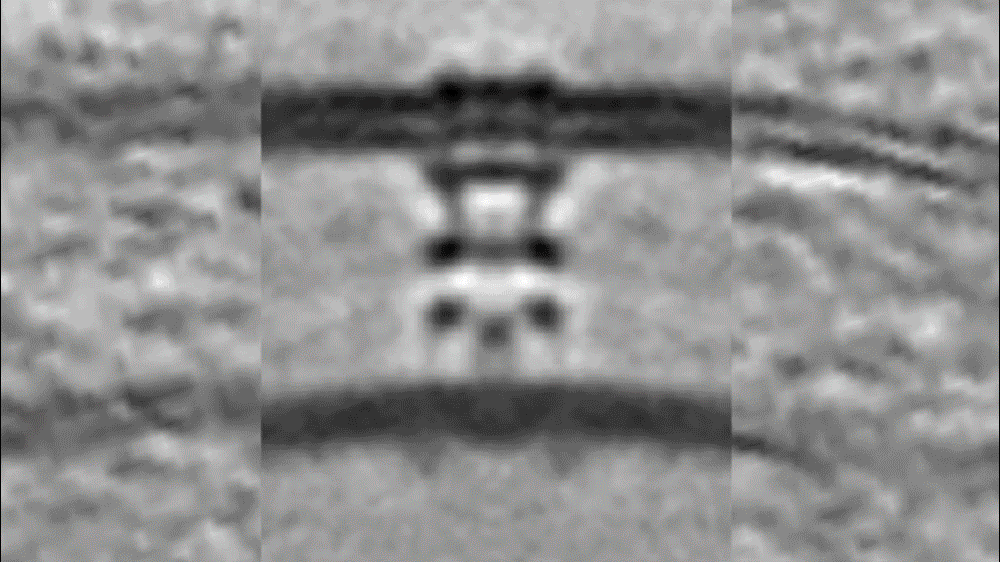
\includegraphics{img/schematics/6_10_1}

A series of rings anchors the Type IV Pilus basal body in the cell envelope. This rigid structure provides leverage for an ATPase at the base to rotate an adaptor in the inner membrane. We think that when it spins in one direction, the adaptor scoops pilin monomers diffusing in the inner membrane into the assembling pilus \citep{chang2016}. Once the pilus has reached its target, attachment is sensed by the basal body (we do not yet know how). As a result, the assembly ATPase dissociates and a second, homologous ATPase takes its place. This disassembly ATPase spins the adaptor in the opposite direction, escorting pilin monomers back into the inner membrane, ready to join the next growing pilus.

\hypertarget{type-ix-secretion-system}{%
\section{Type IX Secretion System}\label{type-ix-secretion-system}}

Other bacteria use different machinery to move over surfaces. \emph{Flavobacterium johnsoniae} like this cell use a Type IX Secretion System to secrete adhesive filaments. These filaments move on a helical track around the cell, and thereby the cell moves forward on a surface. The power for this gliding movement is thought to come from rotary motors anchored in the cell wall that propel the adhesive filaments along their track in a rack-and-pinion fashion, but we still do not understand the mechanism in detail.



\hypertarget{htmlwidget-f950c732218fa3e45840}{}

\label{fig:6-11}\protect\hyperlink{tree}{Flavobacterium johnsoniae} Collected by: \protect\hyperlink{gregory_henderson}{Gregory Henderson} Movie DOI: \href{https://doi.org/10.22002/D1.1535}{10.22002/D1.1535}

\hypertarget{terminal-organelle}{%
\section{Terminal Organelle}\label{terminal-organelle}}

Another, familiar, way to get across a surface is to walk. For this to work, though, you need to be able to change the conformation of your body. This is possible if your cell lacks a cell wall or surface layer, like this \emph{Mycoplasma pneumoniae}. Like the \emph{Mycoplasma genitalium} you saw in Chapter 2--Membrane, these cells are intracellular pathogens, so they do not need to buttress their membrane against differences in osmolarity. As a result, they are soft and flexible. This may allow them to use a leg-like internal structure called a terminal organelle to crawl, or more elegantly ``glide,'' across a surface. The exact mechanism is still unclear, but one possibility is that a hinge-like conformational change in the terminal organelle extends and contracts the back of the cell with respect to the front, similar to the movement of an inchworm (but less exaggerated). Combined with adhesion proteins on the cell surface, this might propel the cell forward.

The skeleton-like terminal organelle gives these cells their characteristic flask shape. In combination with their minimal cell envelope, it can also give rise to an unusual method of cell division. In some species (or genetically engineered strains) that lack the division protein FtsZ, \emph{Mycoplasma} cells still manage to divide. They replicate their terminal organelle normally, as you can see this cell has done, and then the two copies simply walk away from each other, stretching the mother cell between them until the membrane pinchess off to produce two daughters.

Keep in mind that these are simply \emph{some} of the ways we know bacteria and archaea get around, and we continue to discover new ones.



\hypertarget{htmlwidget-bcd0bc3f0c0be4c15395}{}

\label{fig:6-12}\protect\hyperlink{tree}{Mycoplasma pneumoniae} Collected by: \protect\hyperlink{gregory_henderson}{Gregory Henderson} Movie DOI: \href{https://doi.org/10.22002/D1.1536}{10.22002/D1.1536}

\hypertarget{further-reading-5}{%
\section{Further Reading}\label{further-reading-5}}

Albers and Jarrell (2018). \emph{The archaellum: An update on the unique archaeal motility structure} \citep{albers2018}.

Berg (2003). \emph{The rotary motor of bacterial flagella} \citep{berg2003}.

Jarrell and McBride (2008). \emph{The surprisingly diverse ways that prokaryotes move} \citep{jarrell2008}.

Muñoz-Dorado et al. (2016). \emph{Myxobacteria: Moving, killing, feeding, and surviving together} \citep{munoz-dorado2016}.

Shrivastava and Berg (2015). \emph{Towards a model for Flavobacterium gliding} \citep{shrivastava2015}.

\hypertarget{navigation}{%
\chapter{Navigation}\label{navigation}}

\begin{quote}
``\emph{E. coli} forgets where it is going in about 10 seconds.''
- Howard Berg \citep{berg1988}
\end{quote}

\hypertarget{chemotaxis}{%
\section{Chemotaxis}\label{chemotaxis}}

Now that your cell can move, it needs to figure out which way to go. Perhaps it should take a sniff. Chemosensory systems are ancient (they were already present in the common ancestor of bacteria and archaea) and widespread, reflecting their great utility. Chemosensory systems are two-component signaling systems. The first component is a receptor that binds a specific chemical, such as a sugar or amino acid. The binding results in a conformational change that propagates down the long receptor \protect\hyperlink{Chemoreceptor_structure}{Schematic: Chemoreceptor structure}, turning off a kinase bound at the other end that controls the state of the second component: a response regulator. These response regulator proteins then carry the signal elsewhere in the cell by diffusion.

For chemotaxis (``taxis,'' or ordered movement, in response to chemicals) the signal is carried to the cell's motility machinery, usually the flagellar motor, but also type IV pili. Phosphorylated response regulators bind the flagellar motor, switching the direction of rotation. This produces different results depending on the pattern of flagella on the cell. If there is a single flagellum, as on this \emph{Shewanella oneidensis} cell, it switches the flagellum between pushing and pulling the cell body, reorienting the cell in the process. In peritrichously-flagellated cells like \emph{Escherichia coli}, it brings the flagella into and out of a bundle. Remember that bundled flagella drive the cell forward in straight ``runs'' and dissociated flagella ``tumble'' the cell to try a new direction. Constant feedback from the chemosensory system switches the balance of phosphorylated/unphosphorylated response regulator and therefore keeps the cell heading in the general direction of an attractant chemical cue, or away from a repellant.

Chemosensory systems form arrays containing many copies of the proteins. As in this \emph{S. oneidensis} cell, arrays are usually located near the flagella they control, with the tips of the chemoreceptors sticking through the membrane into the periplasm or extracellular space where they can detect signals from the environment. At the other end of the array, the associated kinases interact with the response regulators. These kinases, along with an additional structural protein that helps organize the array, form a layer that we see as a dense line in the cytoplasm.



\hypertarget{htmlwidget-94ea1eddc08326e853c8}{}

\label{fig:7-1}\protect\hyperlink{tree}{Shewanella oneidensis} Collected by: \protect\hyperlink{mohammed_kaplan}{Mohammed Kaplan} Movie DOI: \href{https://doi.org/10.22002/D1.1545}{10.22002/D1.1545}

\hypertarget{Chemoreceptor_structure}{%
\subsection*{Schematic: Chemoreceptor structure}\label{Chemoreceptor_structure}}
\addcontentsline{toc}{subsection}{Schematic: Chemoreceptor structure}

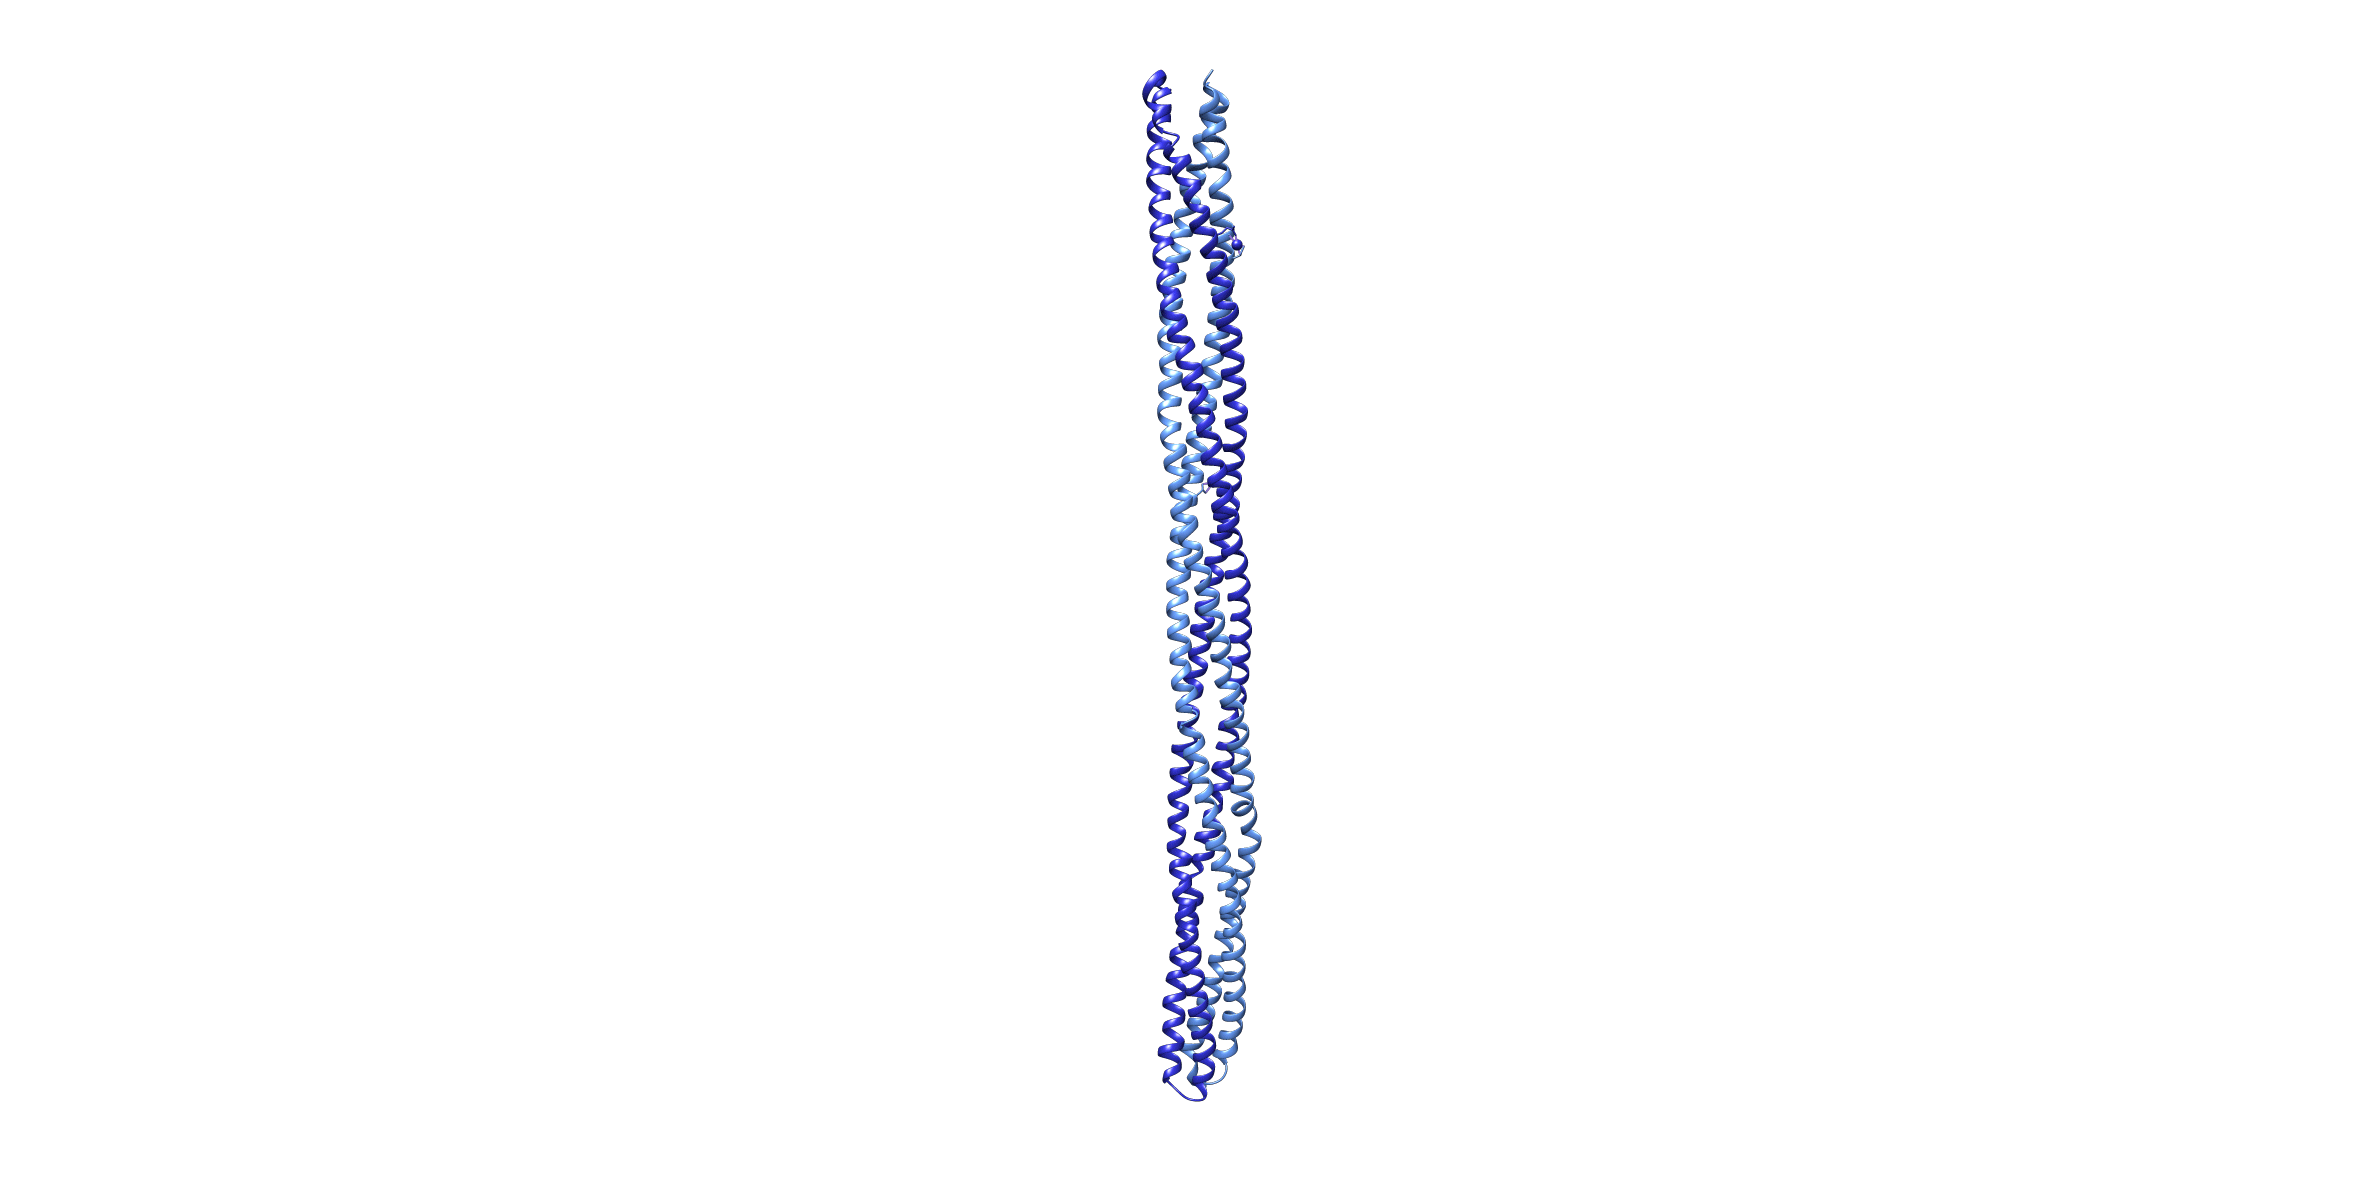
\includegraphics{img/schematics/7_1_1}

\href{http://rcsb.org/structure/2CH7}{\emph{PDB: 2CH7}}
Chemoreceptors take the form of long rods. A single protein zips back along itself, and then joins together with a second copy, forming a rigid bundle of four intertwining helices (two from each member of the dimer), as you can see in this dimer of receptors from \emph{Thermotoga maritima} \citep{park2006}. Only the cytoplasmic portion is shown here; in the cell, the receptors would also have a membrane-embedded anchor at the top and, beyond that, a small domain in the periplasm to bind the chemical of interest. Once a chemical binds, the signal is transmitted down the length of the receptor to a kinase waiting at the distal tip.

\hypertarget{chemosensory-arrays}{%
\section{Chemosensory Arrays}\label{chemosensory-arrays}}

Chemosensory arrays are highly ordered, as you can best see from a bird's-eye view, as in this lysed \emph{Salmonella typhimurium} cell. Chemoreceptors come together as dimers, which in turn organize into trimers, which are further packed into the extensive hexagonal honeycombed array you see here. The hexagonal arrangement comes from the baseplate, where the kinases and coupling proteins bind into an ordered array \protect\hyperlink{Chemosensory_array_architecture}{Schematic: Chemosensory array architecture}. In what should be a familiar theme by now, organization provides a great benefit. Bacteria and archaea have a tremendous sense of smell, responding to as few as one or two molecules of an attractant, or many more. In fact, the range of chemical concentrations they can sense extends over 5 orders of magnitude. But how can a single receptor transmit a signal efficiently? Perhaps it should pass on the message to its neighbors. The interlocking network of chemoreceptors enables just this kind of amplification; a target binding to one receptor may translate into activation of 36 adjacent receptors, enormously boosting the gain of the signal.



\hypertarget{htmlwidget-cff2c544052f750abd7a}{}

\label{fig:7-2}\protect\hyperlink{tree}{Salmonella typhimurium} Collected by: \protect\hyperlink{morgan_beeby}{Morgan Beeby} Movie DOI: \href{https://doi.org/10.22002/D1.1546}{10.22002/D1.1546}

\hypertarget{Chemosensory_array_architecture}{%
\subsection*{Schematic: Chemosensory array architecture}\label{Chemosensory_array_architecture}}
\addcontentsline{toc}{subsection}{Schematic: Chemosensory array architecture}

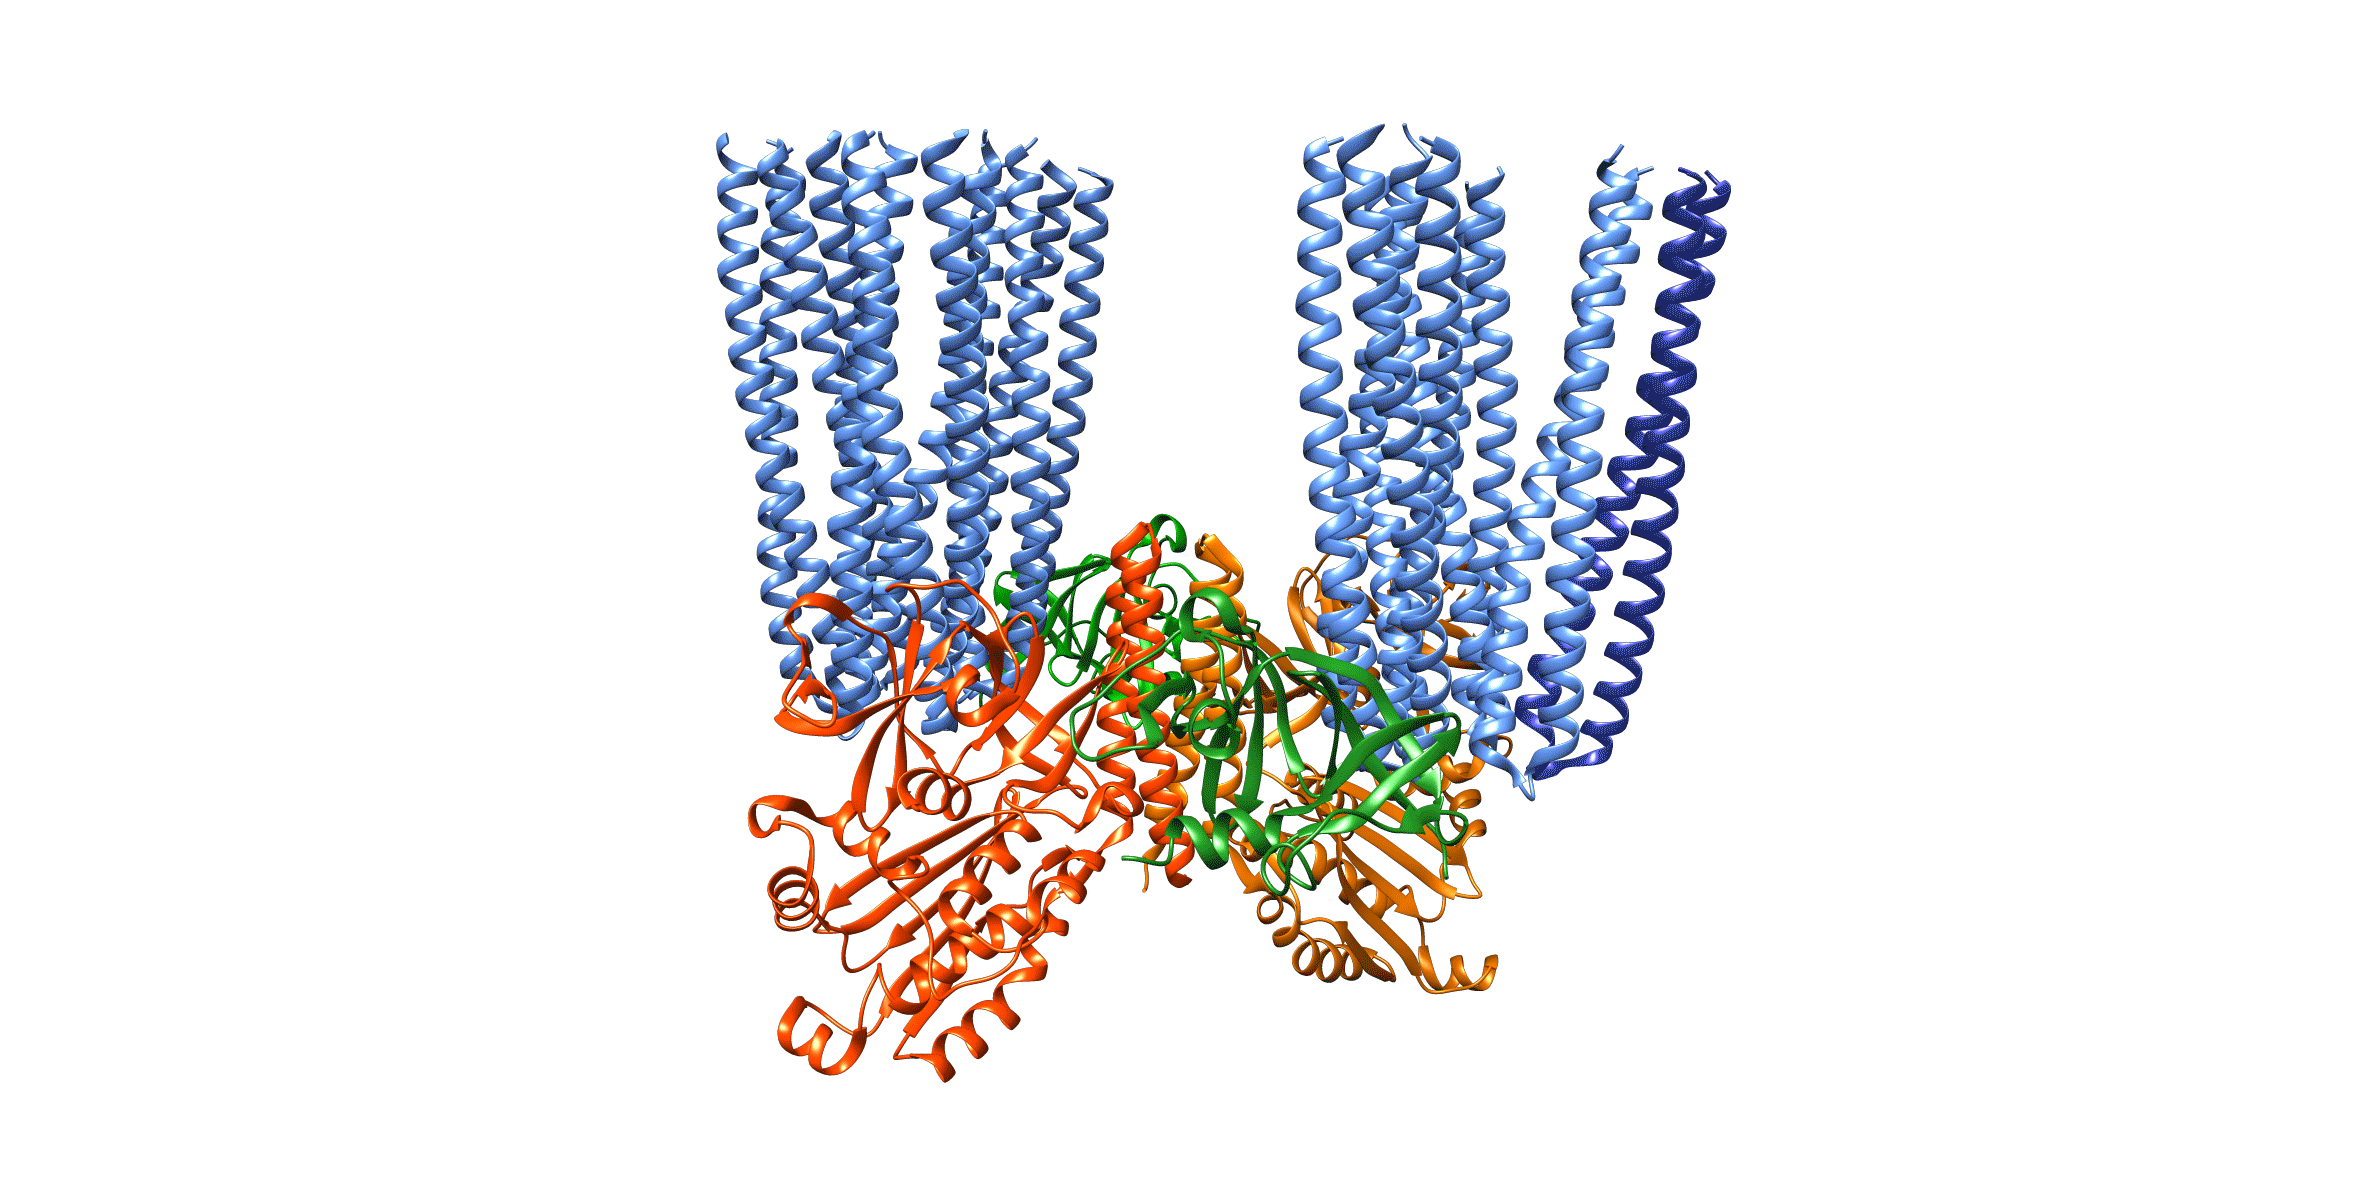
\includegraphics{img/schematics/7_2_1}

\href{http://rcsb.org/structure/6S1K}{\emph{PDB: 6S1K}}
Here you see two of the basic units of a chemosensory array from \emph{Escherichia coli} \citep{cassidy2020}. Each unit consists of a trimer of chemoreceptor dimers (a section of which is shown in blue), a kinase (in orange), and a coupling protein (in green). In the cell, these two units would further associate with four more into a rosette of six units, then with other rosettes, forming the extensive hexagonal array. Also keep in mind that these are just the stable components; additional proteins interact transiently with the receptors and kinases.

\hypertarget{chemosensory-array-conservation}{%
\section{Chemosensory Array Conservation}\label{chemosensory-array-conservation}}

The hexagonal array structure of chemosensory systems is invariant across species, and even across domains. As you can see in this \emph{Methanospirillum hungatei} cell, the arrays have the same architecture in archaea as in bacteria, with 12 nm center-to-center spacing between the hexagons. This strong conservation indicates the importance of chemotaxis for cells' fitness, and suggests that evolution had already honed it to a relatively optimal form in the common ancestor of all these cells.



\hypertarget{htmlwidget-2441dbd5b36d32939ab5}{}

\label{fig:7-3}\protect\hyperlink{tree}{Methanospirillum hungatei} Collected by: \protect\hyperlink{ariane_briegel}{Ariane Briegel} Movie DOI: \href{https://doi.org/10.22002/D1.1547}{10.22002/D1.1547}

\hypertarget{chemoreceptor-variety}{%
\section{Chemoreceptor Variety}\label{chemoreceptor-variety}}

While there is only one architectural style for chemosensory systems, there are many different building materials. Each chemoreceptor senses one, or perhaps two related, types of chemicals. This means that if your cell wants to sense multiple chemicals in its environment, it needs a matching assortment of chemoreceptors. This can quickly get complicated. Some signals need to go to the flagella, some to the pili, and others to the transcriptional machinery to turn on or off genes. How can you keep the wires from getting crossed? The simplest approach is just to separate them, and that seems to be exactly what cells do. Chemoreceptors that signal to different systems have different lengths, which sorts them into separate arrays in the cell, as you can see in this \emph{Vibrio cholerae}. The shorter arrays signal to the flagellar motor, and the longer array signals to a different target we have not yet identified. Even when multiple chemosensory systems signal to the same target, arrays that respond to different environmental cues are kept separate by length differences in the receptors \protect\hyperlink{Azospirillum_brasilense_aerotaxis}{More: Azospirillum brasilense aerotaxis}.



\hypertarget{htmlwidget-97f46afd054e376a8ddb}{}

\label{fig:7-4}\protect\hyperlink{tree}{Vibrio cholerae} Collected by: \protect\hyperlink{ariane_briegel}{Ariane Briegel} Movie DOI: \href{https://doi.org/10.22002/D1.1548}{10.22002/D1.1548}

\hypertarget{Azospirillum_brasilense_aerotaxis}{%
\subsection*{More: Azospirillum brasilense aerotaxis}\label{Azospirillum_brasilense_aerotaxis}}
\addcontentsline{toc}{subsection}{More: Azospirillum brasilense aerotaxis}

A length difference of as little as 2 nm is enough to separate receptors, like these in \emph{Azospirillum brasilense} that sense oxygen (28 nm array) and sources of energy like malate (30 nm array). Both receptors send signals to the single flagellar motor, promoting runs or direction switches to guide the bacterium through a combination of chemotaxis and aerotaxis (ordered movement in an oxygen gradient) to its target: plant roots. \emph{A. brasilense} fixes nitrogen, boosting the growth of plants it colonizes.



\hypertarget{htmlwidget-d6901b1c846a74b7bed5}{}

\label{fig:7-4a}\protect\hyperlink{tree}{Azospirillum brasilense} Collected by: \protect\hyperlink{ariane_briegel}{Ariane Briegel} Movie DOI: \href{https://doi.org/10.22002/D1.1551}{10.22002/D1.1551}

\hypertarget{cytoplasmic-chemosensory-arrays}{%
\section{Cytoplasmic Chemosensory Arrays}\label{cytoplasmic-chemosensory-arrays}}

In addition to their extensive repertoire of membrane-embedded chemoreceptors, cells may also have another type. Many species of bacteria and archaea, like this \emph{Methanoregula formicica}, contain cytoplasmic chemosensory arrays. The receptors lack membrane insertion patches. Instead, they interact end-to-end with each other at their chemical-sensing tips, zippering into a double-layered sandwich, with a baseplate of kinases and coupling proteins on either side. In some species, the arrays are curved like this; in others, they are straight. What these systems sense remains a mystery. One idea is that they monitor the internal state of the cell (e.g.~the levels of various metabolites) to fine-tune signaling responses to meet the current needs of the cell. They are often found along with, and often quite close to, membrane-embedded chemosensory arrays \protect\hyperlink{Vibrio_cholerae_chemosensory_arrays}{More: Vibrio cholerae chemosensory arrays}.



\hypertarget{htmlwidget-3ed42c8b472a2d326012}{}

\label{fig:7-5}\protect\hyperlink{tree}{Methanoregula formicica} Collected by: \protect\hyperlink{ariane_briegel}{Ariane Briegel} Movie DOI: \href{https://doi.org/10.22002/D1.1549}{10.22002/D1.1549}

\hypertarget{Vibrio_cholerae_chemosensory_arrays}{%
\subsection*{More: Vibrio cholerae chemosensory arrays}\label{Vibrio_cholerae_chemosensory_arrays}}
\addcontentsline{toc}{subsection}{More: Vibrio cholerae chemosensory arrays}

This \emph{Vibrio cholerae} cell showcases a full complement of chemosensory systems: an extensive membrane-embedded array (signaling to the flagellar motor) and a cytoplasmic array (signaling to a still-unknown target) . In each case, the basic architecture is identical: hexagonally-arranged trimers of chemoreceptor dimers.



\hypertarget{htmlwidget-132d311091088c502500}{}

\label{fig:7-5a}\protect\hyperlink{tree}{Vibrio cholerae} Collected by: \protect\hyperlink{ariane_briegel}{Ariane Briegel} Movie DOI: \href{https://doi.org/10.22002/D1.1552}{10.22002/D1.1552}

\hypertarget{magnetotaxis}{%
\section{Magnetotaxis}\label{magnetotaxis}}

Chemotaxis is not the only mode of navigation available to your cell. For a clue to others, think about how we orient ourselves in the world. In addition to our nose sniffing out food, we also use our eyes to sense light. Similarly, some photosynthetic bacteria have evolved phototaxis (ordered movement in response to light).

We may also use an external tool to navigate unfamiliar surroundings: a compass. Believe it or not, some bacteria have one, too. Magnetotactic species like this \emph{Magnetospirillum magneticum} have evolved specialized structures called magnetosomes. They are pockets of inner membrane filled with crystals of a magnetic iron mineral like magnetite. The cell organizes the magnetosomes into a line using filaments of a cytoskeletal protein called MamK \protect\hyperlink{MamK_structure}{Schematic: MamK structure}, which is related to eukaryotic actin. The linear chain of magnetosomes functions like the needle of a compass, aligning the cell in a magnetic field.

Magnetosomes first form with the creation of a pocket of inner membrane, as you can see in this cell. Multiple short chains of magnetosomes may form, which are then organized into a single chain by MamK filaments. As mineralization begins, the pockets enlarge to accommodate the growing crystals, ultimately reaching \textasciitilde{}60 nm in diameter. Magnetosome chains are inherited by daughter cells through division. Segregation is relatively easy: the chain spans the division plane so that the inward-growing wedge of cell wall simply splits the chain between magnetosomes, delivering half the chain to each daughter.

Much remains mysterious about these structures. For instance, what forms the membrane pockets? An even bigger question is how cells use their compasses. One theory is that magnetosomes guide the aquatic bacteria vertically to the optimal height in the water column for, e.g.~a certain oxygen level. However, these species are also found at the magnetic equator, where the Earth's field is horizontal. Another hypothesis is that magnetic orientation improves the efficiency of navigation by buffering the cell against Brownian motion that would knock it off course.



\hypertarget{htmlwidget-e0bbd8135ba9af609eec}{}

\label{fig:7-6}\protect\hyperlink{tree}{Magnetospirillum magneticum} Collected by: \protect\hyperlink{zhuo_li}{Zhuo Li} Movie DOI: \href{https://doi.org/10.22002/D1.1550}{10.22002/D1.1550}

\hypertarget{MamK_structure}{%
\subsection*{Schematic: MamK structure}\label{MamK_structure}}
\addcontentsline{toc}{subsection}{Schematic: MamK structure}

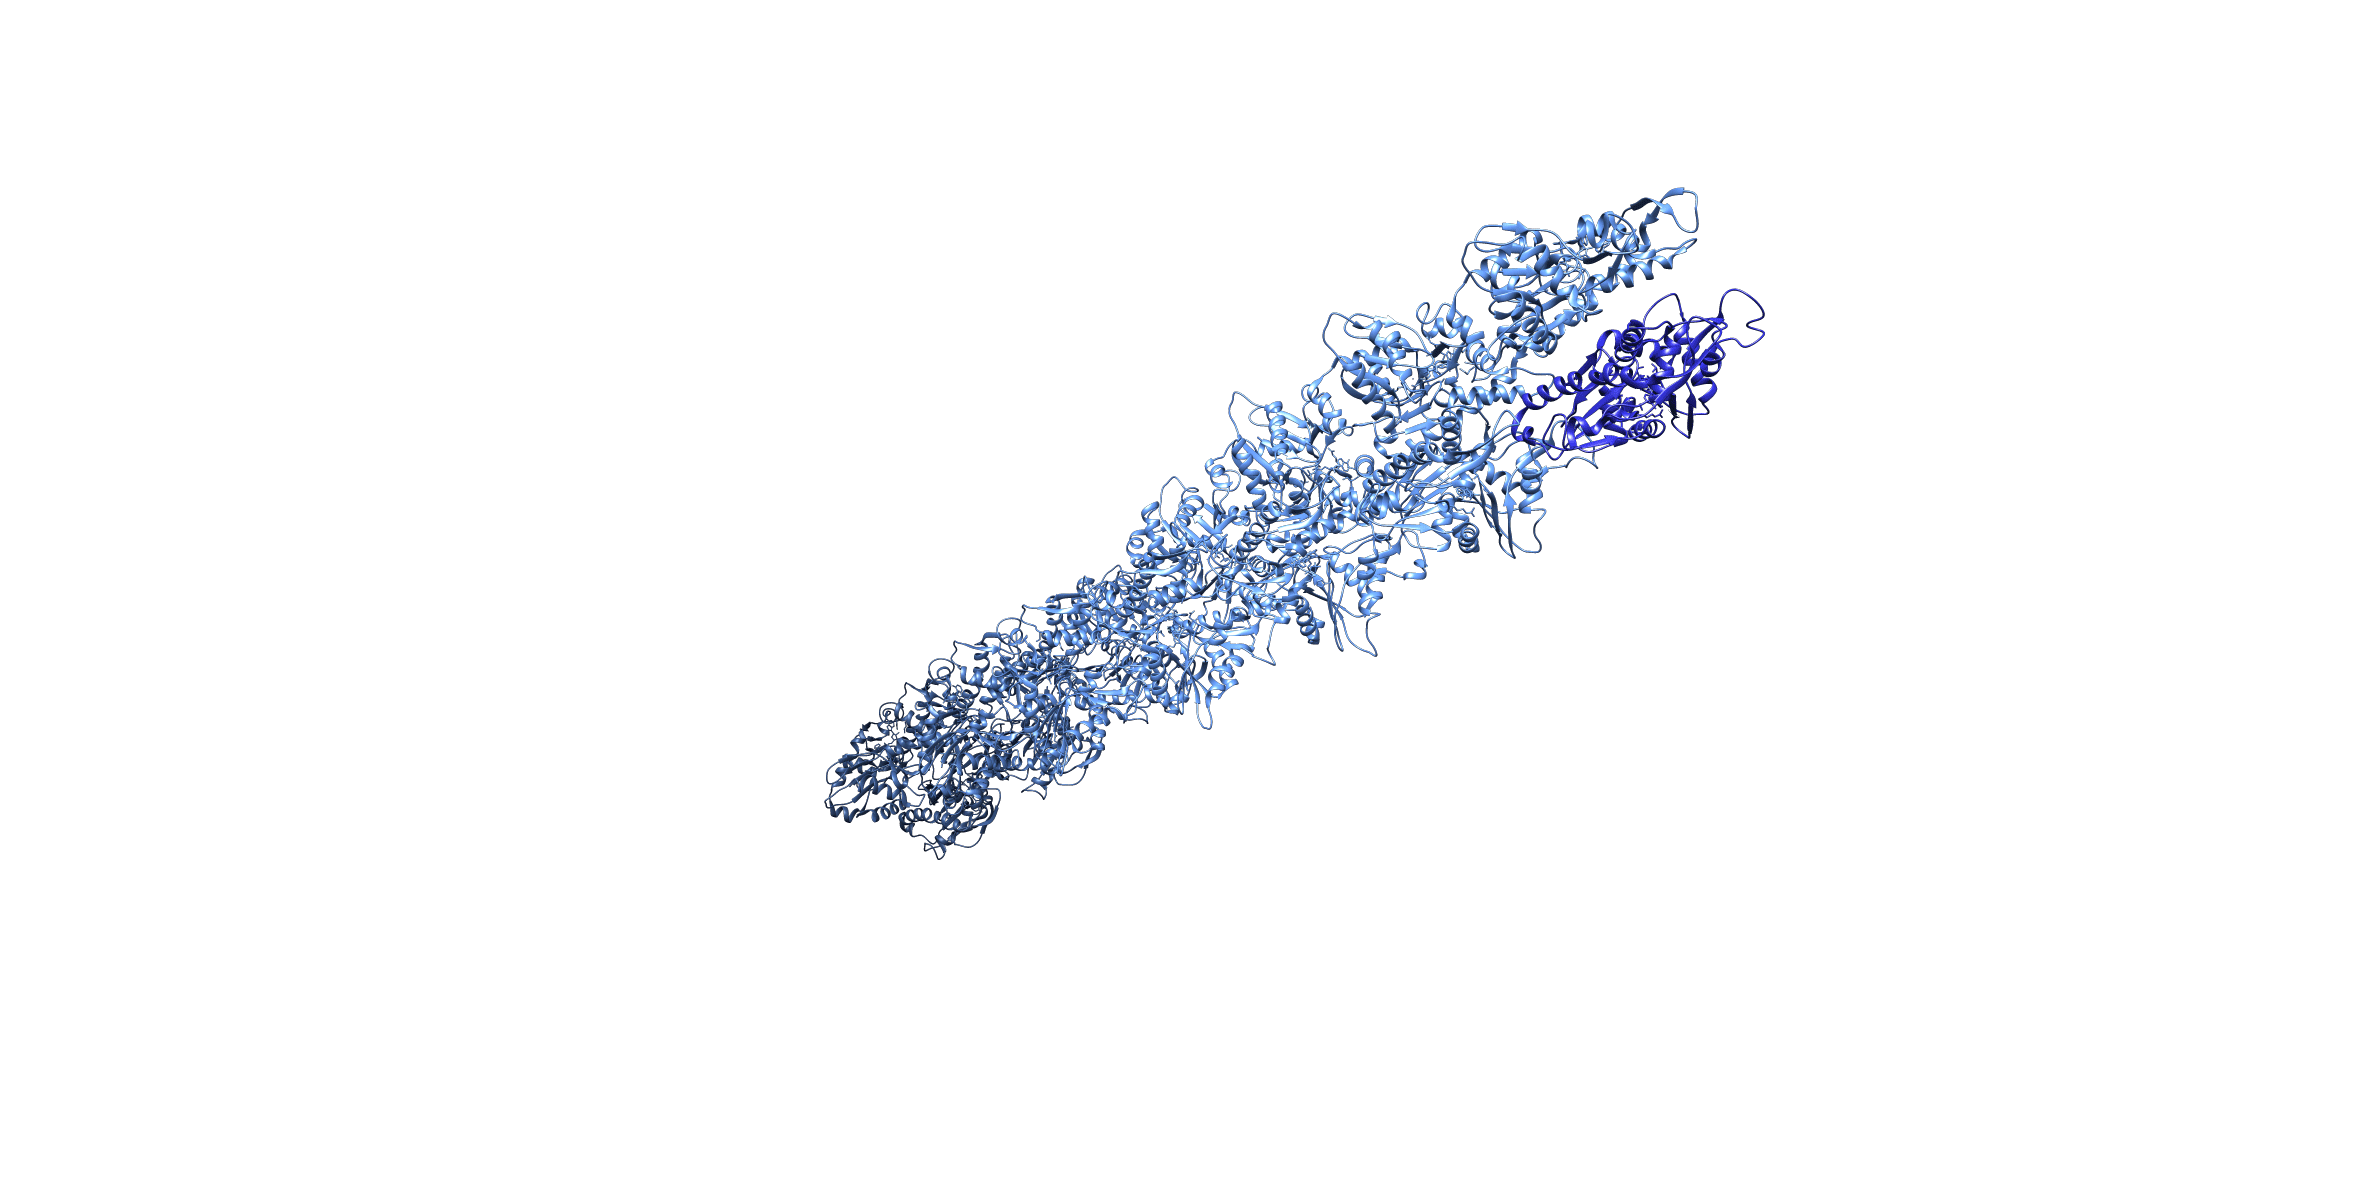
\includegraphics{img/schematics/7_6_1}

\href{http://rcsb.org/structure/5JYG}{\emph{PDB: 5JYG}}
MamK, like its eukaryotic homologue, actin, polymerizes into double-stranded filaments like this one from \emph{Magnetospirillum magneticum} \citep{bergeron2017}. Unlike eukaryotic actin, though, the two strands are in register, rather than being staggered to pack more tightly.

\hypertarget{further-reading-6}{%
\section{Further Reading}\label{further-reading-6}}

Berg (1988). \emph{A physicist looks at bacterial chemotaxis} \citep{berg1988}.

Hazelbauer et al. (2008). \emph{Bacterial chemoreceptors: High-performance signaling in networked arrays} \citep{hazelbauer2008}.

Lower and Bazylinski (2013). \emph{The bacterial magnetosome: A unique prokaryotic organelle} \citep{lower2013}.

Schuergers et al. (2016). \emph{Cyanobacteria use micro-optics to sense light direction} \citep{schuergers2016}.

\hypertarget{lifecycle}{%
\chapter{Lifecycle}\label{lifecycle}}

\begin{quote}
``the microbial world consists almost entirely of bacteria in various degrees of starvation.''
- John Postgate \citep{postgate1994}
\end{quote}

\hypertarget{stationary-phase}{%
\section{Stationary Phase}\label{stationary-phase}}

Your cell is fairly well optimized now. It can grow, divide, and find fuel to repeat the process. But what happens when there is no food is to be found? Natural environments offer famine more often than feast. And conditions can become harsh (high temperature, low pH, little water). For minor shortages of carbon or phosphate, your cell can fall back on its storage granules. But what about more prolonged starvation or stress? To outlast these conditions, your cell would do well to hunker down and conserve its remaining energy. Cells have evolved just such a mechanism: a stationary (non-growing) state. When conditions are no longer optimal for growth, the cell stops protein production and compacts its nucleoid to protect the DNA from damage, as you can see in this \emph{Caulobacter crescentus}. The cell also shrinks its cytoplasm either by dividing at a smaller size, or by digesting nonessential components and cinching down its membrane (stressed cells often contain more cytoplasmic vesicles). Some diderm bacteria, including \emph{C. crescentus}, also remodel their cell walls and outer membranes (releasing extracellular vesicles). Others, like \emph{Escherichia coli}, do not, resulting in a larger periplasm. In stationary phase, rod-shaped cells become more round. Nonessential protein assemblies are lost; note the missing surface layer on this cell. When cells no longer have energy to spare to power motility, they also lose their flagella (see them floating next to these cells) and dismantle their chemosensory arrays. The cell now plays a waiting game. If the environment changes, your cell can resume active growth. Or the death of a neighboring cell, like the one you see here, might release a burst of nutrients that your cell can use for one more round of growth and division, producing progeny that might find a better life. Unlike in a well-maintained laboratory culture, in Nature bacteria and archaea spend most of their time in stationary phase, awaiting fleeting opportunities for growth.



\hypertarget{htmlwidget-4d21de747c7141448a0e}{}

\label{fig:8-1}\protect\hyperlink{tree}{Caulobacter crescentus} Collected by: \protect\hyperlink{prabha_dias}{Prabha Dias} Movie DOI: \href{https://doi.org/10.22002/D1.1553}{10.22002/D1.1553}

\hypertarget{genome-protection}{%
\section{Genome Protection}\label{genome-protection}}

Remember that the most critical part of your cell is its instruction manual--the genome. Ensuring that the instructions remain intact is paramount to your cell in stationary phase. To do this, all cells have proteins (RecA in bacteria, RadA in archaea, and Rad51 in eukaryotes) that repair DNA damage caused by reactive oxygen species, UV (or other) radiation, heat, or other sources. RecA (and related) proteins form complexes with the DNA they protect. These ordered arrays can become quite extensive in stationary phase cells, like this \emph{Helicobacter pylori}.

This cell exhibits other hallmarks of stationary phase: its shrinking membranes have produced vesicles and it has shed its flagella. It has not yet (at least fully) digested its chemosensory array. Note also the relatively weak association of the outer membrane with this pathogenic diderm, allowing the cell to curl up inside.



\hypertarget{htmlwidget-bb51a932edaac4113c34}{}

\label{fig:8-2}\protect\hyperlink{tree}{Helicobacter pylori} Collected by: \protect\hyperlink{yi-wei_chang}{Yi-Wei Chang} Movie DOI: \href{https://doi.org/10.22002/D1.1554}{10.22002/D1.1554}

\hypertarget{archaeal-stationary-phase}{%
\section{Archaeal Stationary Phase}\label{archaeal-stationary-phase}}

Stationary phase in archaea looks much the same as in bacteria, as you can see in this \emph{Thermococcus kodakaraensis}. The cell has shrunk to about half its size in active growth, partly by shedding vesicles, and much of the surface layer has been dismantled. It has lost its archaella (though the conical plate in the cytoplasm remains) and degraded its chemosensory array, and is protecting its genome with RadA filaments. Now it waits for things to get better.



\hypertarget{htmlwidget-b43a5d5b857bcf8590ec}{}

\label{fig:8-3}\protect\hyperlink{tree}{Thermococcus kodakaraensis} Collected by: \protect\hyperlink{debnath_ghosal}{Debnath Ghosal} Movie DOI: \href{https://doi.org/10.22002/D1.1555}{10.22002/D1.1555}

\hypertarget{differentiation}{%
\section{Differentiation}\label{differentiation}}

While all cells go through cycles of growth and quiescence in response to changes in their environment, some species have gone a step further to evolve a programmed set of states--a lifecycle. In some cases, as you will see in the next chapter, a lifecycle allows bacteria to prey efficiently on other cells, including ours. In other cases, such as these \emph{Caulobacter crescentus}, it allows the bacterium to thrive in an environment with low nutrient levels. \emph{C. crescentus} has a dimorphic (``two form'') lifecycle. Newborn cells start out life as swarmers, with a polar flagellum. They swim through the environment (either freshwater or saltwater) until they (hopefully) reach a favorable spot to put down roots, which they do by first transiently attaching to a surface with pili, then making the attachment permanent with a polymer of a sticky protein called ``holdfast,'' which currently holds the record for the strongest known biological adhesive \protect\hyperlink{Holdfast}{More: Holdfast}. They shed their flagellum and grow a stalk in its place. Only after growing a stalk, completing the process of differentiation, will the cell begin to divide. The stalked cell will remain attached to the surface for the rest of its life, dividing asymmetrically to produce new swarmer cells, which swim away to try their luck elsewhere. Here you see a swarmer cell on the bottom, and a stalked cell on the top, in the process of dividing to produce another swarmer that would swim off to the right. You saw a similar dimorphic lifecycle in Chapter 5, in sessile (non-motile) \emph{Hyphomonas neptunium} that bud to produce motile daughters. This kind of lifecycle helps prevent related cells from competing with one another for scarce local nutrients.



\hypertarget{htmlwidget-568d0a69760a0d0fcb2f}{}

\label{fig:8-4}\protect\hyperlink{tree}{Caulobacter crescentus} Collected by: \protect\hyperlink{zhuo_li}{Zhuo Li} Movie DOI: \href{https://doi.org/10.22002/D1.1556}{10.22002/D1.1556}

\hypertarget{Holdfast}{%
\subsection*{More: Holdfast}\label{Holdfast}}
\addcontentsline{toc}{subsection}{More: Holdfast}

\emph{Prosthecobacter vanneervenii} is a stalked bacterium like \emph{Caulobacter crescentus}, and attaches to surfaces by the same mechanism: a sticky ball of holdfast at the tip of its stalk. Here you see four cells whose stalks have attached to one another. Unlike its cousin \emph{C. crescentus}, however, \emph{P. vanneervenii} is non-motile (no flagellum) and does not have a dimorphic life cycle. It divides symmetrically.



\hypertarget{htmlwidget-b7b64ae27d6c256abaf1}{}

\label{fig:8-4a}\protect\hyperlink{tree}{Prosthecobacter vanneervenii} Collected by: \protect\hyperlink{martin_pilhofer}{Martin Pilhofer} Movie DOI: \href{https://doi.org/10.22002/D1.1564}{10.22002/D1.1564}

\hypertarget{sporulation}{%
\section{Sporulation}\label{sporulation}}

The strategies we just discussed can help your cell deal with lean times. But what if things get \emph{really} bad? Maybe you need to build your cell a survivalist bunker. Several species of bacteria do just this, using a modified cell division program to create a special reinforced daughter cell called a spore. Spores are extremely resistant to dehydration, acid, heat and other dangers. They are a purely dormant cell form, neither growing nor dividing, but simply waiting for improved conditions.

Some bacterial species form exospores, which are released directly to the environment as in a normal division. Others, like monoderm \emph{Bacillus subtilis}, form endospores, which mature inside the protective envelope of the mother cell. As you can see in this cell, the first step resembles an asymmetric (closer to one pole) but otherwise normal cell division, with a septum of cell wall separating the compartment that will become the spore. Unlike in regular monoderm division, though, in which the septum is the same thickness as the rest of the cell wall, the sporulation septum is thinner, containing fewer layers of peptidoglycan. Also unlike division, the septum seems to form very rapidly \protect\hyperlink{Sporulation_septum_formation}{More: Sporulation septum formation}.

\emph{Note that this cell (and the ones on the next two pages) is narrower than normal }B. subtilis\emph{; a cell wall remodeling enzyme has been removed from its genome, leaving essential functions like cell wall growth and division (and sporulation) intact, but making the cells narrower and therefore better to image by cryoET.}



\hypertarget{htmlwidget-edcfe283e2e813cb8169}{}

\label{fig:8-5}\protect\hyperlink{tree}{Bacillus subtilis} Collected by: \protect\hyperlink{elitza_tocheva}{Elitza Tocheva} Movie DOI: \href{https://doi.org/10.22002/D1.1557}{10.22002/D1.1557}

\hypertarget{Sporulation_septum_formation}{%
\subsection*{More: Sporulation septum formation}\label{Sporulation_septum_formation}}
\addcontentsline{toc}{subsection}{More: Sporulation septum formation}

From hundreds of sporulating \emph{Bacillus subtilis} we imaged by cryoET, this is the only cell captured in the process of forming a septum. As you can see, it is at a very early stage in the process. The fact that we do not see more intermediates suggests that once the septum starts to form, it quickly proceeds to completion.



\hypertarget{htmlwidget-34c7e98a841a86706dd3}{}

\label{fig:8-5a}\protect\hyperlink{tree}{Bacillus subtilis} Collected by: \protect\hyperlink{elitza_tocheva}{Elitza Tocheva} Movie DOI: \href{https://doi.org/10.22002/D1.1565}{10.22002/D1.1565}

\hypertarget{sporulation-contd.}{%
\section{Sporulation (cont'd.)}\label{sporulation-contd.}}

Once the septum is in place, it is then extended, as you can see in this \emph{Bacillus subtilis} cell, enlarging the nascent spore and ultimately separating it from the mother cell envelope. Note that the monoderm mother is producing a diderm spore, surrounded by two layers of its mother's membrane. As this occurs, a copy of the genome is pumped through a specialized protein nanomachine. The increased turgor pressure from the highly-concentrated DNA helps the spore round and expand. Usually, the mother cell membrane closes off at the cell pole, but occasionally this occurs instead on the side of the mother cell \protect\hyperlink{Spore_engulfment}{More: Spore engulfment}.

When the process of engulfment is finished, the spore's cell wall is reinforced and expanded into a tough ``cortex,'' and an extra protein coat is added to the outside, completing the sturdy envelope that will protect the spore from harsh environments \protect\hyperlink{Spore_coating}{More: Spore coating}. Finally, when the spore is ready, the mother cell lyses, releasing the time capsule to its fate.



\hypertarget{htmlwidget-2c7e7b8d268e798ff99e}{}

\label{fig:8-6}\protect\hyperlink{tree}{Bacillus subtilis} Collected by: \protect\hyperlink{elitza_tocheva}{Elitza Tocheva} Movie DOI: \href{https://doi.org/10.22002/D1.1558}{10.22002/D1.1558}

\hypertarget{Spore_engulfment}{%
\subsection*{More: Spore engulfment}\label{Spore_engulfment}}
\addcontentsline{toc}{subsection}{More: Spore engulfment}

The process of spore engulfment by the mother cell membrane culminates in closure of the membranes, creating an outer spore membrane and an inner spore membrane on either side of the sporulation septum. The final point of separation is usually at the center of the cell pole, but not always, as you can see in this \emph{Bacillus subtilis} spore being engulfed from the side of the mother cell. The layer to the right of the developing spore may be a precursor of the coat \protect\hyperlink{Spore_coating}{More: Spore coating}.



\hypertarget{htmlwidget-129b304f9703180a3bf0}{}

\label{fig:8-6a}\protect\hyperlink{tree}{Bacillus subtilis} Collected by: \protect\hyperlink{elitza_tocheva}{Elitza Tocheva} Movie DOI: \href{https://doi.org/10.22002/D1.1566}{10.22002/D1.1566}

\hypertarget{Spore_coating}{%
\subsection*{More: Spore coating}\label{Spore_coating}}
\addcontentsline{toc}{subsection}{More: Spore coating}

In this later stage of sporulation, you can see that the \emph{Bacillus subtilis} spore has now separated completely from the mother cell envelope. It has also moved away from the cell pole. The layer flanking the spore may be the assembling spore coat.



\hypertarget{htmlwidget-6ce8c4d6264bada93ee1}{}

\label{fig:8-6b}\protect\hyperlink{tree}{Bacillus subtilis} Collected by: \protect\hyperlink{elitza_tocheva}{Elitza Tocheva} Movie DOI: \href{https://doi.org/10.22002/D1.1567}{10.22002/D1.1567}

\hypertarget{spores}{%
\section{Spores}\label{spores}}

Fully mature \emph{Bacillus subtilis} spores like this one are ovoid, and swollen with armor, including the thick cortex and multilayered coat. This dense shield protects the cargo within from drying out, or denaturing in heat or acid. (It also makes it hard to make out much internal detail in images.)

Once released, the spore will remain dormant as long as necessary, protected by its carbohydrate and protein armor, waiting for optimal conditions of water, temperature and pH to germinate. The wait can be long, sometimes very, very, \emph{very} long. In one case, \emph{Bacillus subtilis} spores were revived from a salt crystal thought to have formed 250 million years ago.



\hypertarget{htmlwidget-4527c82de3acad038c7f}{}

\label{fig:8-7}\protect\hyperlink{tree}{Bacillus subtilis} Collected by: \protect\hyperlink{elitza_tocheva}{Elitza Tocheva} Movie DOI: \href{https://doi.org/10.22002/D1.1559}{10.22002/D1.1559}

\hypertarget{germination}{%
\section{Germination}\label{germination}}

When conditions become conducive to growth, the spore will return to a vegetative state, shedding its protein coat and outer membrane and dismantling its cortex to allow outgrowth of the now-active cell, as you see in this reviving (or ``germinating'') \emph{Bacillus subtilis} spore.

The ready transition between a monoderm cell with a thick cell wall and a diderm spore with a thin septal wall may provide a hint to the origin of diderm bacterial cells. Perhaps a spore, maybe released prematurely from its mother before its septum had thickened into a full cortex, kept growing and dividing with both membranes and a thin cell wall. Evolution could then tinker with the second membrane, specializing it into the modern bacterial outer membrane.



\hypertarget{htmlwidget-b5fee365f74c106bf978}{}

\label{fig:8-8}\protect\hyperlink{tree}{Bacillus subtilis} Collected by: \protect\hyperlink{elitza_tocheva}{Elitza Tocheva} Movie DOI: \href{https://doi.org/10.22002/D1.1560}{10.22002/D1.1560}

\hypertarget{diderm-sporulation}{%
\section{Diderm Sporulation}\label{diderm-sporulation}}

Sporulation is not limited to monoderms. A few species of diderm bacteria also form spores (some exospores and others endospores). The process is much the same as in monoderms, despite the different cell envelope structure. It begins with an asymmetric septum close to one pole of the cell, as you can see in this \emph{Acetonema longum}. As in monoderms, the septum contains a thin layer of peptidoglycan (remember that diderms have a thin cell wall, though, so the thickness is about the same).



\hypertarget{htmlwidget-c8b628a6a8e400928b99}{}

\label{fig:8-9}\protect\hyperlink{tree}{Acetonema longum} Collected by: \protect\hyperlink{elitza_tocheva}{Elitza Tocheva} Movie DOI: \href{https://doi.org/10.22002/D1.1561}{10.22002/D1.1561}

\hypertarget{diderm-sporulation-contd.}{%
\section{Diderm Sporulation (cont'd.)}\label{diderm-sporulation-contd.}}

Engulfment also proceeds similarly, as you can see in this \emph{Acetonema longum} cell, with the septum expanding and moving to cinch off at the pole of the mother cell \protect\hyperlink{Complete_engulfment}{More: Complete engulfment}. As the cell wall is remodeled to accomplish this, the rod shape of the mother is lost. Note also how the outer membrane of the mother cell ruffles and expands, apparently having detached from the cell wall. Compared to a daughter cell produced by division, there is something quite interesting about the envelope of the endospore. Look carefully at the membranes. Both the inner and outer membranes of the spore derive from the inner membrane of the mother cell. This implies a surprising interchangeability of the two membrane types, and lends further credence to the idea that the outer membrane of some or all diderm bacteria originally came from a monoderm spore that failed to shed its second membrane.

As you saw in \emph{Bacillus subtilis}, once engulfment is complete, the thin septal wall will be expanded and reinforced into a thick cortex and a protective protein coat will be added before the mature spore is released by lysis of the mother cell \protect\hyperlink{Mature_spore}{More: Mature spore}. \emph{A. longum} spores are round, but other rod-shaped diderms form ovoid spores \protect\hyperlink{Sporomusa_acidovorans_sporulation}{More: Sporomusa acidovorans sporulation}.



\hypertarget{htmlwidget-eb29fc049df21809c53b}{}

\label{fig:8-10}\protect\hyperlink{tree}{Acetonema longum} Collected by: \protect\hyperlink{elitza_tocheva}{Elitza Tocheva} Movie DOI: \href{https://doi.org/10.22002/D1.1562}{10.22002/D1.1562}

\hypertarget{Complete_engulfment}{%
\subsection*{More: Complete engulfment}\label{Complete_engulfment}}
\addcontentsline{toc}{subsection}{More: Complete engulfment}

This \emph{Acetonema longum} cell has completed engulfment, creating a ``forespore.'' \emph{Acetonema longum} forespores (and mature spores) typically contain several granules, likely storing poly-phosphate. These may help power outgrowth when the spore germinates. Spores from other species, though, like \emph{Bacillus subtilis}, do not contain obvious storage granules, so they may serve another, species-specific role.



\hypertarget{htmlwidget-9fe1350715a2cfeba357}{}

\label{fig:8-10a}\protect\hyperlink{tree}{Acetonema longum} Collected by: \protect\hyperlink{elitza_tocheva}{Elitza Tocheva} Movie DOI: \href{https://doi.org/10.22002/D1.1568}{10.22002/D1.1568}

\hypertarget{Mature_spore}{%
\subsection*{More: Mature spore}\label{Mature_spore}}
\addcontentsline{toc}{subsection}{More: Mature spore}

This mature \emph{Acetonema longum} spore has been released by lysis of its mother cell. Note its extensive armor: a thick cortex between the membranes, and a multilayered protein coat.



\hypertarget{htmlwidget-ea379fd6ed8d8865b982}{}

\label{fig:8-10b}\protect\hyperlink{tree}{Acetonema longum} Collected by: \protect\hyperlink{elitza_tocheva}{Elitza Tocheva} Movie DOI: \href{https://doi.org/10.22002/D1.1569}{10.22002/D1.1569}

\hypertarget{Sporomusa_acidovorans_sporulation}{%
\subsection*{More: Sporomusa acidovorans sporulation}\label{Sporomusa_acidovorans_sporulation}}
\addcontentsline{toc}{subsection}{More: Sporomusa acidovorans sporulation}

This diderm \emph{Sporomusa acidovorans} cell is in the process of forming an ovoid endospore. Note also what may be an early stage of cortex formation at the end of the spore, as well as novel structures at the points of cell wall remodeling. We do not know what they are, but they may be involved in engulfment.



\hypertarget{htmlwidget-8fc9e482f41d8640ba5f}{}

\label{fig:8-10c}\protect\hyperlink{tree}{Sporomusa acidovorans} Collected by: \protect\hyperlink{elitza_tocheva}{Elitza Tocheva} Movie DOI: \href{https://doi.org/10.22002/D1.1570}{10.22002/D1.1570}

\hypertarget{diderm-germination}{%
\section{Diderm Germination}\label{diderm-germination}}

Again, when the spore encounters favorable conditions, it will germinate, as this \emph{Acetonema longum} spore is doing. Unlike the \emph{Bacillus subtilis} you saw earlier, germinating diderm spores do not shed their outer membrane. Instead, they remodel their cortex back into a thin cell wall (compare to the mature spore on the previous page). This process is a good reminder of the similarity of monoderm and diderm cell walls; they may look very different, but their fundamental architecture is the same, just with more sheets of material in monoderms (and spores). After the remodel, the cell then sheds its protein coat, as you see here, and starts to grow.

Some archaea also have resistant forms similar to bacterial spores. For instance, when water levels drop in its salty environment, rod-shaped \emph{Halobacterium salinarum} uses a variant division process to produce three or four hardy spherical cells that can survive dormant in halite crystals for tens of thousands of years, awaiting water to revive.

Sporulation may seem like a highly specialized function practiced by relatively few species, but there is reason to think that it may have evolved long ago and been key to the success of life on Earth. Conditions today are extremely clement compared to what they likely were a few billion years ago, when the last common ancestor of all modern cells (called LUCA, for Last Universal Common Ancestor) may have lived. It is quite possible that LUCA was a spore, the only form of life hardy enough to survive conditions volatile and violent enough to kill off the spore's ancestors. If so, most modern lineages of bacteria and archaea simply lost the ability to form spores when it was no longer essential to their survival. It is further possible that a LUCA spore was formed by a cell somewhere else in the solar system and delivered to Earth on one of the asteroids that bombarded the planet in its infancy. We may never know, but the possibilities are fun to consider.



\hypertarget{htmlwidget-1ced21eea9821a1a2bf6}{}

\label{fig:8-11}\protect\hyperlink{tree}{Acetonema longum} Collected by: \protect\hyperlink{elitza_tocheva}{Elitza Tocheva} Movie DOI: \href{https://doi.org/10.22002/D1.1563}{10.22002/D1.1563}

\hypertarget{further-reading-7}{%
\section{Further Reading}\label{further-reading-7}}

Fendrihan et al. (2006). \emph{Extremely halophilic archaea and the issue of long-term microbial survival} \citep{fendrihan2006}.

Pletnev et al. (2015). \emph{Survival guide: Escherichia coli in the stationary phase} \citep{pletnev2015}.

Tocheva et al. (2016). \emph{Sporulation, bacterial cell envelopes and the origin of life} \citep{tocheva2016}.

Vreeland et al. (2000). \emph{Isolation of a 250 million-year-old halotolerant bacterium from a primary salt crystal} \citep{vreeland2000}.

\hypertarget{interaction}{%
\chapter{Interaction}\label{interaction}}

\begin{quote}
``We do not have solitary beings. Every creature is, in some sense, connected to and dependent on the rest.''
- Lewis Thomas \citep{thomas1974}
\end{quote}

\hypertarget{biofilms}{%
\section{Biofilms}\label{biofilms}}

So far we have largely ignored a major part of a cell's environment: other organisms. Your cell is far from alone out there. It shares space and resources with cells of the same species (some its own mothers/sisters/daughters), other species, and even other domains. Think about strategies that could help your cell thrive in such a crowded world. For starters, why can't we all just get along? Cooperation is common in Nature, often in the form of biofilms--communal groups of microorganisms. Biofilms offer advantages to their members, shielding cells on the interior from harsh conditions or antibiotics, and ensuring that nutrients produced by cells' metabolism or released by their death are readily available to others. Biofilms should be familiar to you; think of the scum on your teeth, or the nearest pond. In fact, the earliest physical evidence we have of life on earth is in the form of stromatolites (``layered rocks'')--meter-scale fossilized biofilms of cyanobacteria (you can see still-growing stromatolites in Shark Bay, Australia).

To attach to a biofilm, cells use strategies we have already discussed, including pili and holdfast. \emph{Agrobacterium tumefaciens} like this one use a holdfast-like polymer called Unipolar polysaccharide, or UPP. Some bacteria, including this one, also contribute to the superstructure of the biofilm by secreting cellulose fibers that help form the non-living matrix of the community.



\hypertarget{htmlwidget-254687ced05ddd09f2b2}{}

\label{fig:9-1}\protect\hyperlink{tree}{Agrobacterium tumefaciens} Collected by: \protect\hyperlink{elitza_tocheva}{Elitza Tocheva} Movie DOI: \href{https://doi.org/10.22002/D1.1571}{10.22002/D1.1571}

\hypertarget{biofilms-contd.}{%
\section{Biofilms (cont'd.)}\label{biofilms-contd.}}

Individual cellulose fibers associate into bundles to form a 3D matrix for the cells, as you can see in this thin slice through a \emph{Gluconacetobacter hansenii} biofilm. Not all biofilms contain cellulose, but all have an extracellular matrix, typically made of proteins secreted by the component cells. These proteins have properties that help cells aggregate, like the unipolar polysaccharide you just saw. They may also have other properties useful to the community; for instance, \emph{Bacillus subtilis} secretes a hydrophobic protein that forms a resistant coat around the biofilm. Matrices also contain lipids and extracellular DNA, and dead cells contribute material to the superstructure. Keep in mind that the lab-grown biofilm you see here consists of a single species, but in Nature a biofilm often contains multiple species.



\hypertarget{htmlwidget-f20544d41b63180d94c3}{}

\label{fig:9-2}\protect\hyperlink{tree}{Gluconacetobacter hansenii} Collected by: \protect\hyperlink{william_nicolas}{William Nicolas} Movie DOI: \href{https://doi.org/10.22002/D1.1572}{10.22002/D1.1572}

\hypertarget{type-ii-and-type-iv-secretion}{%
\section{Type II and Type IV Secretion}\label{type-ii-and-type-iv-secretion}}

How else might your cell deal with the crowd? Well, if you can't join them, maybe you should try to beat (and eat) them. Bacteria have evolved an impressive arsenal of molecular weaponry. In fact, most of the antibiotics we use were invented by bacteria. In many cases, cells simply release these antibiotics to the environment, either directly or in membrane vesicles, which may travel further. For more specific targeting, though, cells employ a varied array of secretion systems. You already saw some of these nanomachines in Chapter 6: a type III secretion system assembles the flagellum and a type II secretion system makes (and unmakes) type IV pili. Other family members have evolved more militaristic functions.

Type II secretion systems (T2SSs) in \emph{Legionella pneumophila} like this pump out effector proteins that enable a complex pathogenic lifecycle. \emph{L. pneumophila} live in several environments: inside amoebae, outside cells (but sometimes with others in biofilms), and inside \emph{our} cells, where they cause the severe pneumonia known as Legionnaires' disease. In each environment, the T2SS pumps out proteins that facilitate growth there. For instance, once we inhale \emph{L. pneumophila} with water droplets, they are internalized by our macrophages. They then use their T2SSs to secrete proteins that prevent their pockets in the cell (called \emph{Legionella}-containing vacuoles) from being degraded, and suppress our innate immune response. This gives the bacteria time to replicate and establish a persistent colony. The T2SSs also secrete a toxin protein that breaks down lung tissue.

Unlike the secretion systems in Chapter 6, the T2SS does not build an extracellular appendage. Instead, it is thought to work by pumping proteins through the envelope channel using a short piston-like ``pseudo-pilus'' \protect\hyperlink{Legionella_T2SS_structure}{Schematic: Legionella T2SS structure}, pushing the molecules into the extracellular space. (Keep in mind that for these intracellular pathogens, their extracellular space is the interior of the host cell.)

\emph{L. pneumophila} also use another, unrelated machine, a type IV secretion system (T4SS), to deliver more than 400(!) different kinds of effector proteins into host cells to promote infection. You can see multiple T4SSs primed for action in this cell \protect\hyperlink{Legionella_T4SS_structure}{Schematic: Legionella T4SS structure}. We do not yet know what they look like during active secretion, so the mechanism remains unclear. In another human pathogen, \emph{Helicobacter pylori}, inactive T4SSs are sometimes seen next to mysterious extracellular tubes, raising the intriguing possibility that the structures are somehow related \protect\hyperlink{Helicobacter_pylori_tubes}{More: Helicobacter pylori tubes}.

This \emph{L. pneumophila} cell is not unusual; it is common for pathogenic bacteria to employ multiple types of secretion systems. The bristling arsenal of bacteria is a fearsome thing.



\hypertarget{htmlwidget-b98e3103a4bb799948be}{}

\label{fig:9-3}\protect\hyperlink{tree}{Legionella pneumophila} Collected by: \protect\hyperlink{debnath_ghosal}{Debnath Ghosal} Movie DOI: \href{https://doi.org/10.22002/D1.1573}{10.22002/D1.1573}

\hypertarget{Legionella_T2SS_structure}{%
\subsection*{Schematic: Legionella T2SS structure}\label{Legionella_T2SS_structure}}
\addcontentsline{toc}{subsection}{Schematic: Legionella T2SS structure}

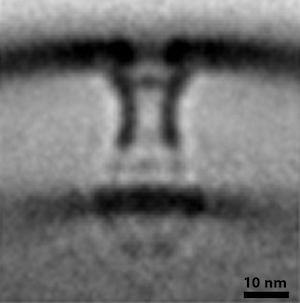
\includegraphics{img/schematics/9_3_1}

\href{https://www.ebi.ac.uk/pdbe/entry/emdb/EMD-20712}{\emph{EMD-20712}} \href{https://www.ebi.ac.uk/pdbe/entry/emdb/EMD-20713}{\emph{EMD-20713}}
This average of type II secretion systems from many \emph{Legionella pneumophila} cells shows the overall structure: a channel through the cell envelope, gated near the outer membrane \citep{ghosal2019}. The pseudo-pilus can be seen in individual T2SSs, extending from the inner membrane to the bottom of the main channel. It gets washed out in the average, though, indicating that it is relatively flexible (i.e.~not always in the same position). We still need to figure out exactly how the system works, including whether the pseudo-pilus does act like a piston, and how the gate opens.

\hypertarget{Legionella_T4SS_structure}{%
\subsection*{Schematic: Legionella T4SS structure}\label{Legionella_T4SS_structure}}
\addcontentsline{toc}{subsection}{Schematic: Legionella T4SS structure}

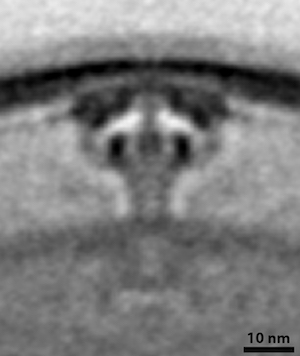
\includegraphics{img/schematics/9_3_2}

\href{https://www.ebi.ac.uk/pdbe/entry/emdb/EMD-0566}{\emph{EMD-0566}}
This average of type IV secretion systems from many \emph{Legionella pneumophila} cells shows the overall structure \citep{ghosal2019a}. We do not yet know how secretion works, but one possibility is that effectors are transported either straight through the channel from the cytoplasm and/or first into the periplasm and from there into the windowed chamber just inside the outer membrane before finally being escorted out of the cell.

\hypertarget{Helicobacter_pylori_tubes}{%
\subsection*{More: Helicobacter pylori tubes}\label{Helicobacter_pylori_tubes}}
\addcontentsline{toc}{subsection}{More: Helicobacter pylori tubes}

This \emph{Helicobacter pylori} cell was cultured together with human gastric epithelial cells, its target for infection. It contains inactive type IV secretion systems, as well as several mysterious tubes. The tubes are formed from the outer membrane, but we do not know what scaffolds them (they have a consistent diameter of 37 nm), or what makes the portals along their length. The fact that we sometimes see tubes near primed T4SSs, and the fact that the tubes are missing from mutant cells lacking T4SS components suggests a relationship, but the details are unclear. Much remains mysterious about this structure and its potential role in infection.



\hypertarget{htmlwidget-07ba7d77bf7cd804c250}{}

\label{fig:9-3a}\protect\hyperlink{tree}{Helicobacter pylori} Collected by: \protect\hyperlink{yi-wei_chang}{Yi-Wei Chang} Movie DOI: \href{https://doi.org/10.22002/D1.1582}{10.22002/D1.1582}

\hypertarget{type-iii-secretion}{%
\section{Type III Secretion}\label{type-iii-secretion}}

What if your cell wanted to go a step further and deliver toxins directly into its target? Perhaps it needs a syringe. One of the most common, and best-studied, pathogenic secretion systems is the type III secretion system (T3SS) that assembles a needle-like toxin delivery system called the injectisome. T3SS injectisomes and flagellar motors are closely related, and the basal machines have similar structures \protect\hyperlink{Injectisome_structure}{Schematic: Injectisome structure}. Rather than assembling a long helical filament for motility, though, injectisomes form a shorter needle, which you can see on this \emph{Pseudomonas aeruginosa}. The needle can penetrate a eukaryotic cell, delivering effectors directly into its cytoplasm that block the immune response of the host, and lead to cell lysis.

\emph{It would be wasteful, or detrimental, for your cell to secrete toxins all the time. Pathogens typically have multi-stage lifecycles, often passing through an intermediate host and/or the environment. Pathogenic machinery like secretion systems are typically only produced when conditions signal that the cell has reached its target (e.g.~increased temperature or salt concentration). Until then, the genes encoding the protein components are turned off. This cell is missing a protein (ExsD) that turns off expression of these injectisome components. As a result, the strain makes injectisomes even outside the host, enabling us to image their structure.}

T3SSs are closely related to type II secretion systems (T2SSs) and share a common element: the channel embedded in the outer membrane, formed by many copies of a protein called a Secretin \protect\hyperlink{Secretin_structure}{Schematic: Secretin structure}. As you can see, though, the rest of the machine looks very different.



\hypertarget{htmlwidget-21ba2d73d6ac8917497f}{}

\label{fig:9-4}\protect\hyperlink{tree}{Pseudomonas aeruginosa} Collected by: \protect\hyperlink{steven_wang}{Steven Wang} Movie DOI: \href{https://doi.org/10.22002/D1.1574}{10.22002/D1.1574}

\hypertarget{Injectisome_structure}{%
\subsection*{Schematic: Injectisome structure}\label{Injectisome_structure}}
\addcontentsline{toc}{subsection}{Schematic: Injectisome structure}

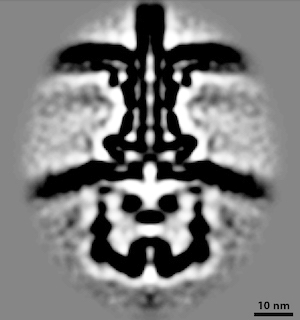
\includegraphics{img/schematics/9_4_1}

\href{https://www.ebi.ac.uk/pdbe/entry/emdb/EMD-20611}{\emph{EMD-20611}}
This average of T3SS injectisomes from many \emph{Shigella flexneri} cells shows the overall structure, including the large ``sorting platform'' in the cytoplasm which selects proteins for secretion through the channel of the needle \citep{tachiyama2019}.

\hypertarget{Secretin_structure}{%
\subsection*{Schematic: Secretin structure}\label{Secretin_structure}}
\addcontentsline{toc}{subsection}{Schematic: Secretin structure}

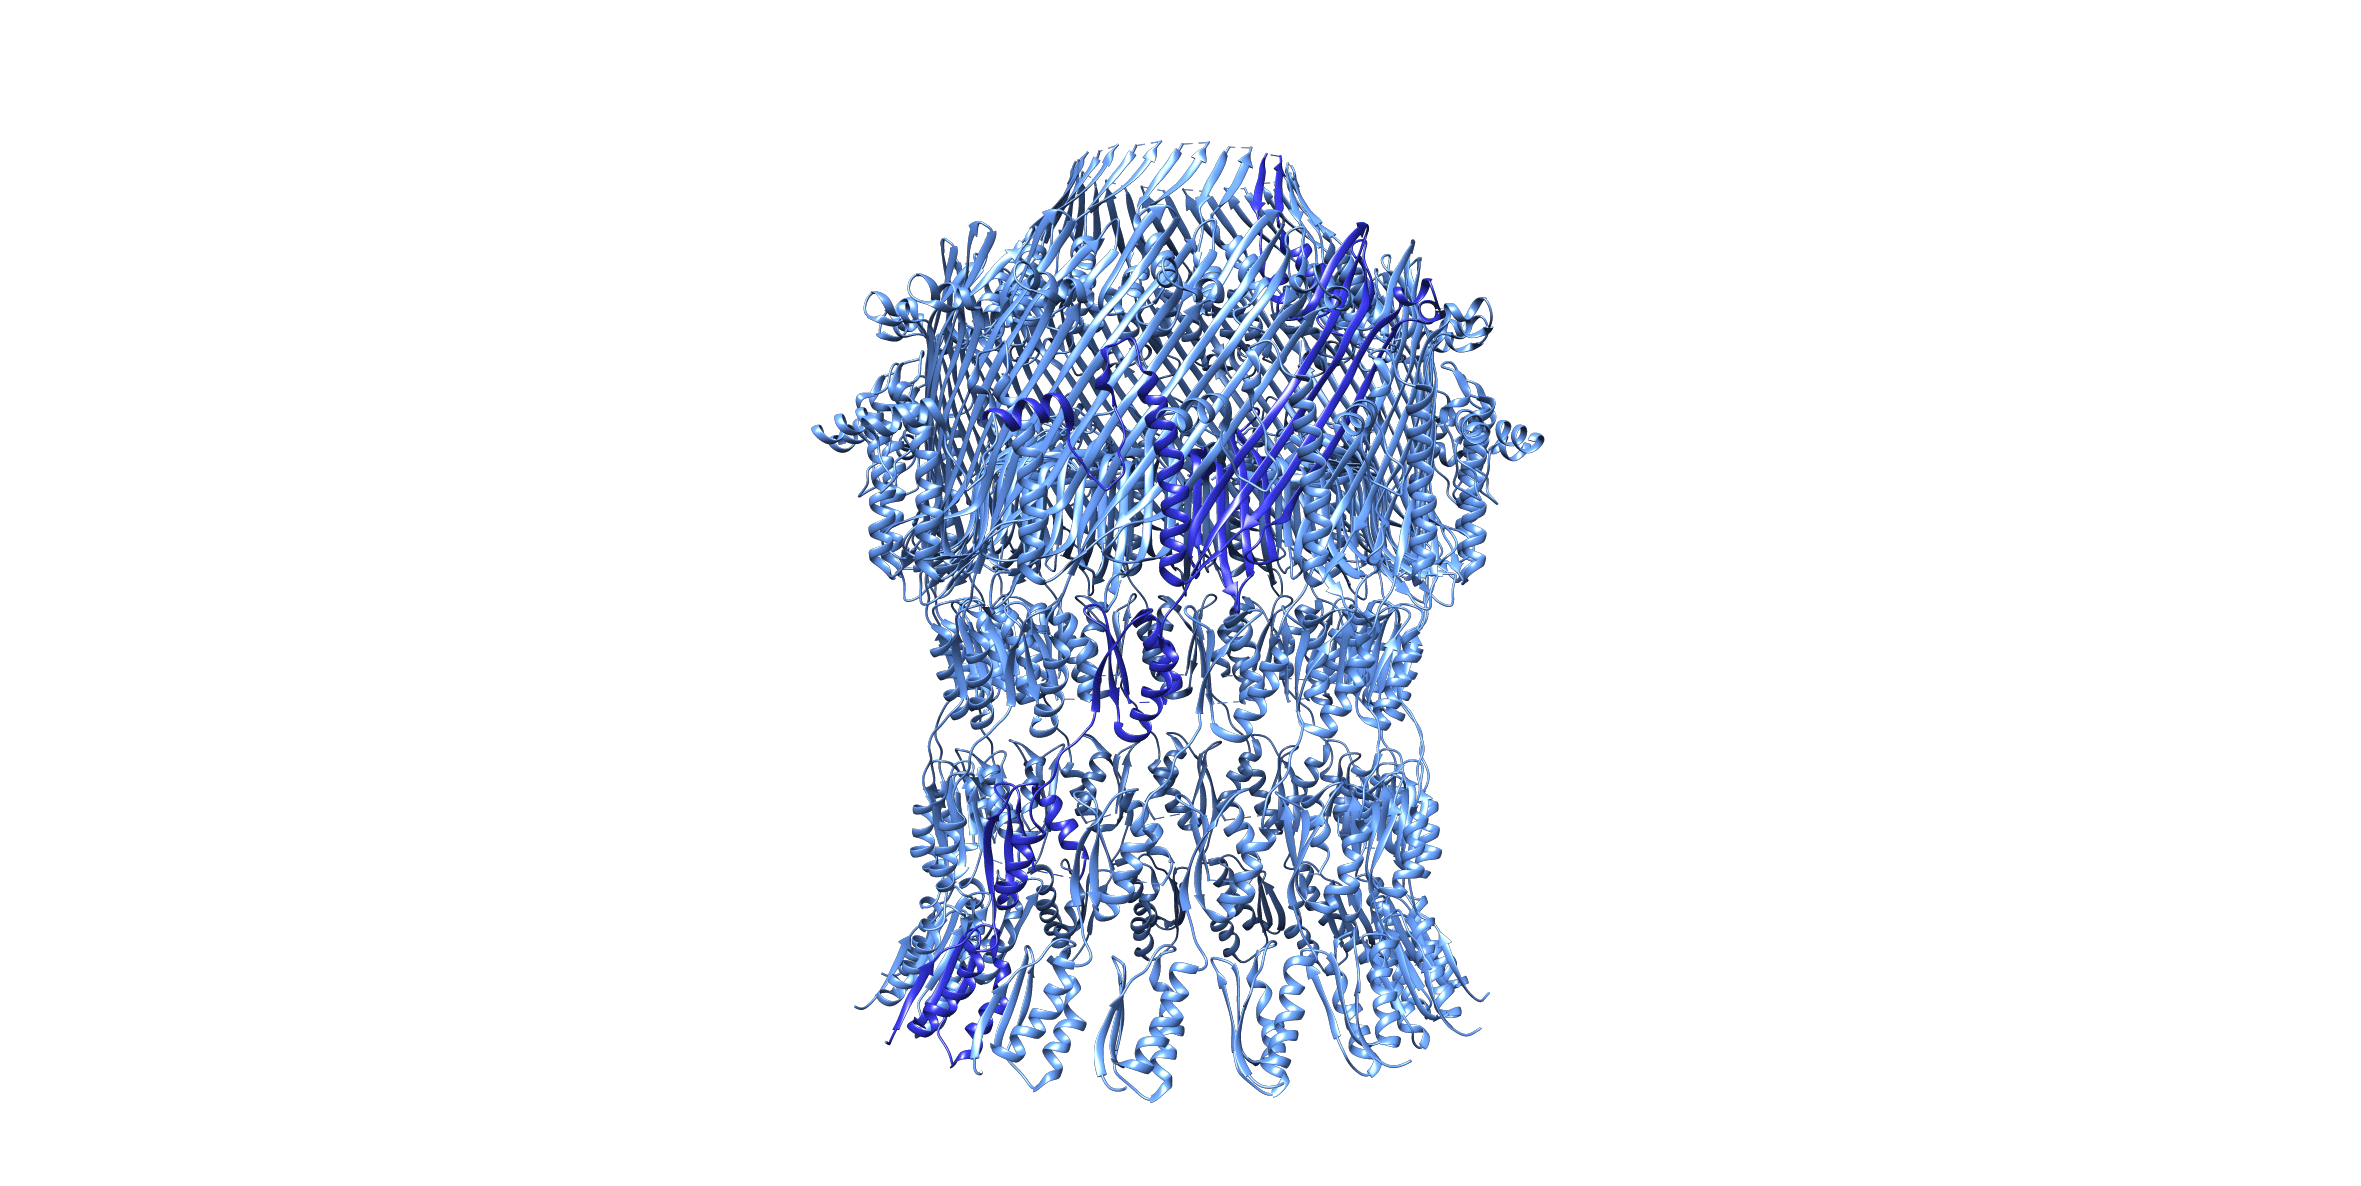
\includegraphics{img/schematics/9_4_2}

\href{http://rcsb.org/structure/5WQ8}{\emph{PDB: 5WQ8}}
Many copies of a Secretin protein come together to form a channel, as in this one from \emph{Vibrio cholerae} \citep{yan2017a}. In addition to the main channel situated in the outer membrane, different domains of the protein form a series of rings in the periplasm that interact with other components of the system.

\hypertarget{type-v-secretion}{%
\section{Type V Secretion}\label{type-v-secretion}}

Other secretion systems independently evolved similar mechanisms, though using very different structures. Some strains of \emph{Escherichia coli} have an ability, called ``Contact-Dependent Inhibition'' or CDI, to inhibit the growth of neighboring diderm bacterial cells. They do this by coopting a pore in the outer membrane of the target cell to introduce a toxin that halts its growth. To safeguard themselves, they make an antitoxin that binds to the toxin and renders it harmless. Such antidote system are common for microbe-produced toxins.

To deliver the toxin to the target, the cells use type V secretion systems (T5SSs) like the ones on this \emph{Escherichia coli}. In contrast to the nanomachines you have been seeing, which contain dozens of unique components, this system is elegantly spare: a channel formed by several copies of one protein (CdiB) in the outer membrane secretes another protein, CdiA. Or rather, it secretes half of it. The first half of CdiA forms the stick you see here, with the second half keeping the toxin domain at the end of the protein sequestered in the periplasm. The tip of the stick contains the domain that recognizes and docks to the receptor pore on the target. When it bumps into a neighboring cell and locks on, the second half of CdiA is secreted, whipping the toxin like a tetherball into the other cell.

\emph{This cell belongs to a strain that is normally incapable of CDI, but has been genetically engineered to produce the T5SS components. Once again, this lets us image the machines more easily; in this case, the CDI-practicing strain has a thicker layer of extracellular proteins, which obscures the needles in a visual haystack.}



\hypertarget{htmlwidget-6c5cd0806ac39d18d12a}{}

\label{fig:9-5}\protect\hyperlink{tree}{Escherichia coli} Collected by: \protect\hyperlink{poorna_subramanian}{Poorna Subramanian} Movie DOI: \href{https://doi.org/10.22002/D1.1575}{10.22002/D1.1575}

\hypertarget{type-vi-secretion}{%
\section{Type VI Secretion}\label{type-vi-secretion}}

How else could your cell deliver a toxin to a nearby competitor? As usual, Nature has provided another, even more entertaining, option: the poison dart gun. Many diderm bacteria, including \emph{Myxococcus xanthus} like this, use type VI secretion systems (T6SSs) to launch effector proteins into neighboring cells. The effectors vary--from toxins that cause lysis to factors that promote biofilm formation. The target range of the T6SS is similarly broad, including monoderm and diderm bacteria and eukaryotic cells.

This primed T6SS consists of a hollow outer tube, with a narrower dart inside \protect\hyperlink{Primed_T6SS_structure}{Schematic: Primed T6SS structure}. The effector protein is loaded at the tip of the dart, where the machine is anchored in the cell envelope. In a few cells, including this one, we see additional filaments flanking the primed T6SS. They are lacking in other cells even of the same species, and their identity and function remain unknown.



\hypertarget{htmlwidget-1eedf4f9703c3c7f411f}{}

\label{fig:9-6}\protect\hyperlink{tree}{Myxococcus xanthus} Collected by: \protect\hyperlink{yi-wei_chang}{Yi-Wei Chang} Movie DOI: \href{https://doi.org/10.22002/D1.1576}{10.22002/D1.1576}

\hypertarget{Primed_T6SS_structure}{%
\subsection*{Schematic: Primed T6SS structure}\label{Primed_T6SS_structure}}
\addcontentsline{toc}{subsection}{Schematic: Primed T6SS structure}

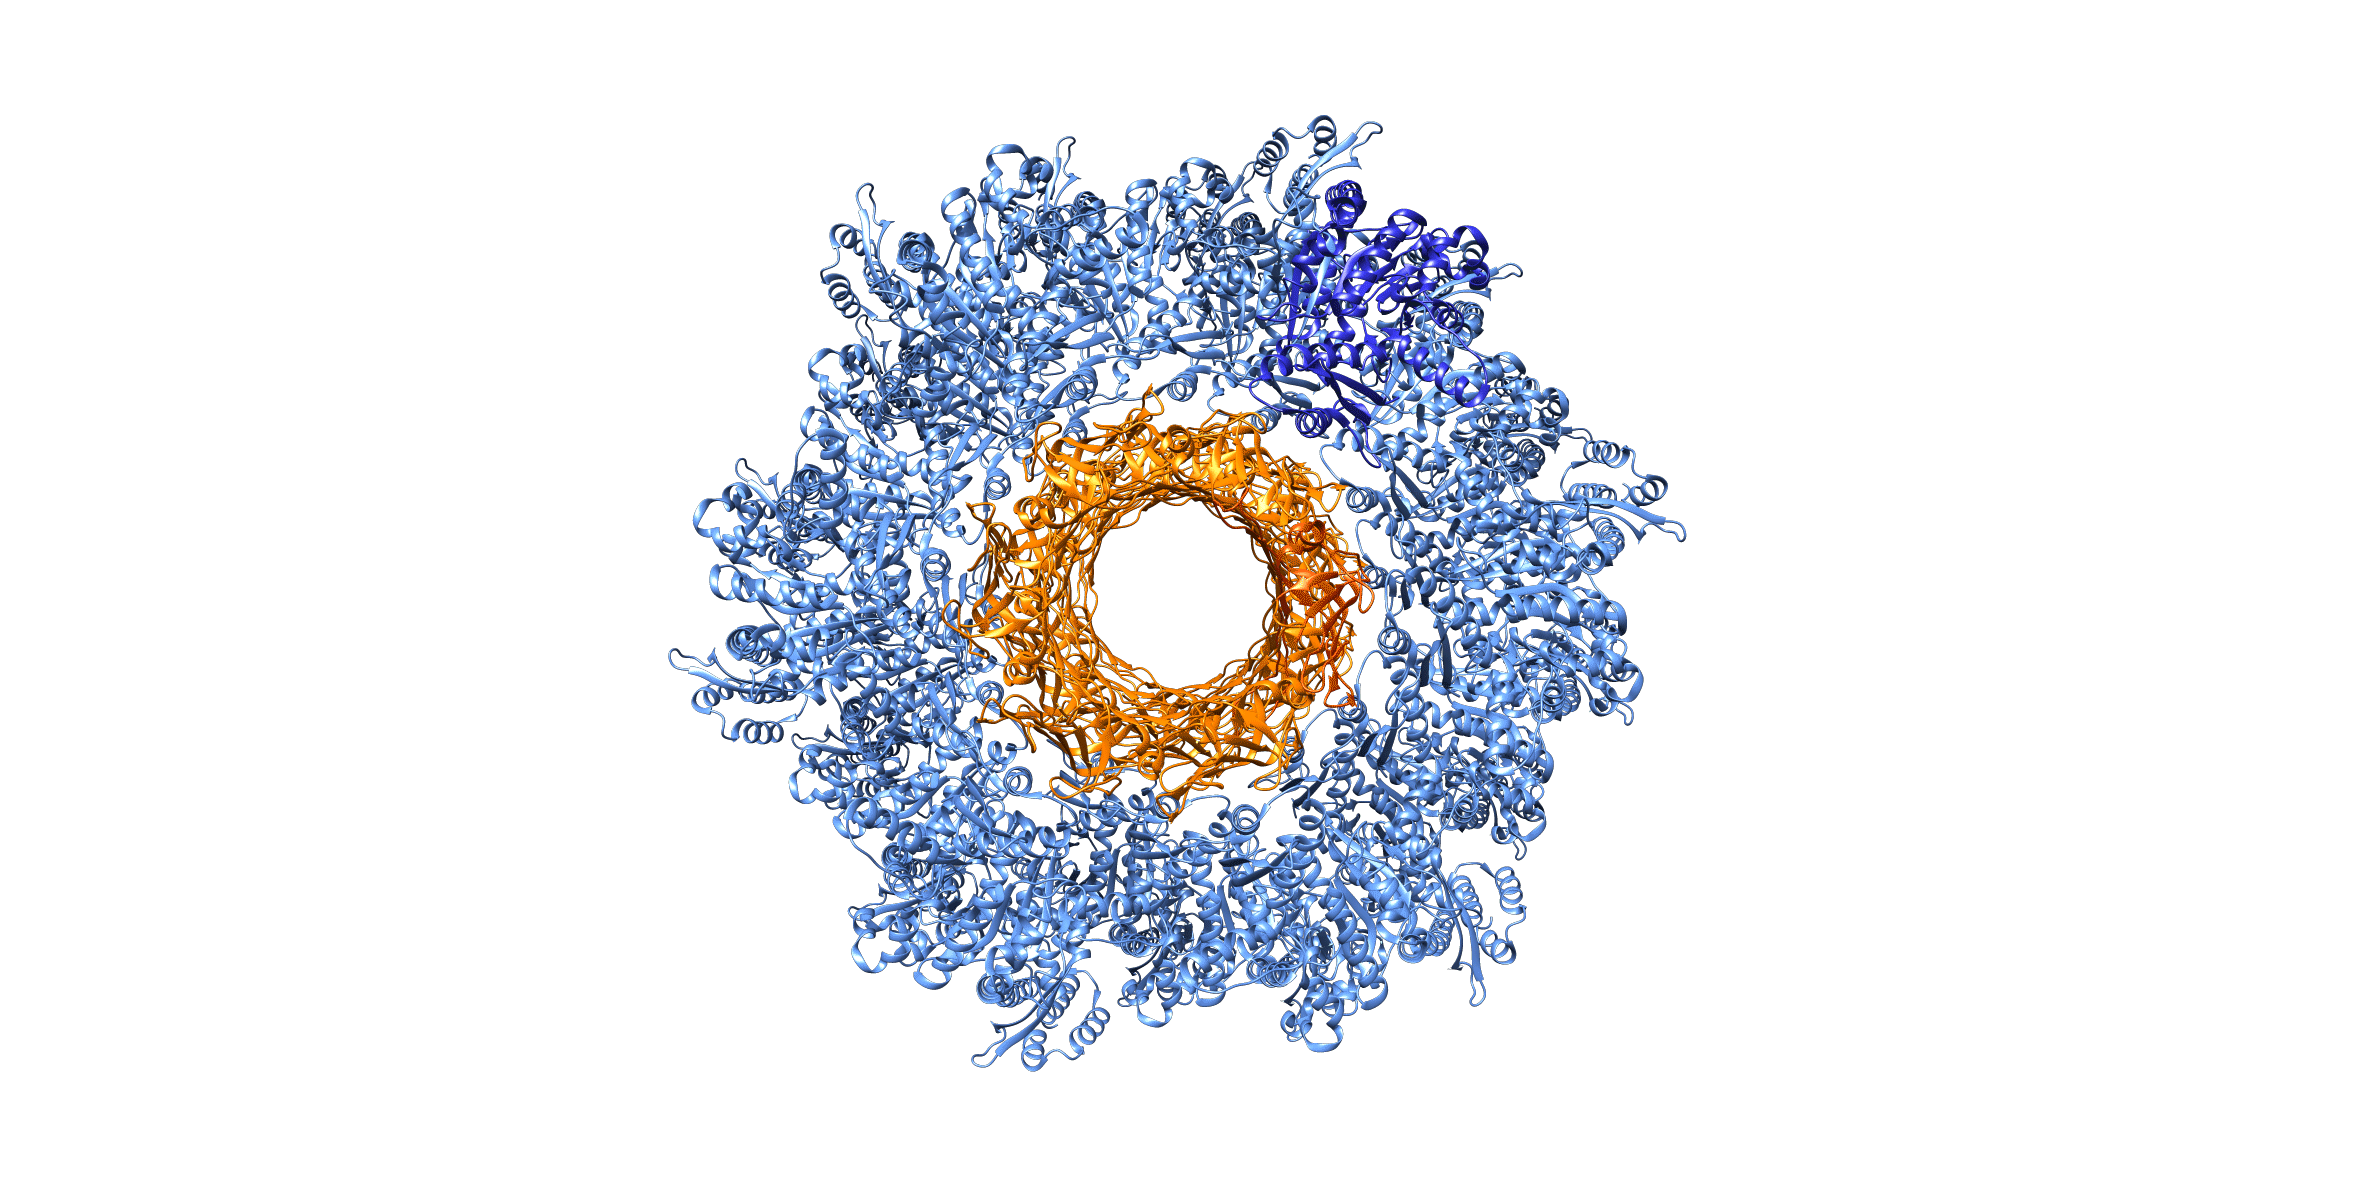
\includegraphics{img/schematics/9_6_1}

\href{http://rcsb.org/structure/5URW}{\emph{PDB: 5URW}}
In a primed T6SS, the projectile rod (orange) nests inside the contractile sheath (blue), as in this section of a T6SS from \emph{Myxococcus xanthus} \citep{chang2017}.

\hypertarget{type-vi-secretion-contd.}{%
\section{Type VI Secretion (cont'd.)}\label{type-vi-secretion-contd.}}

When the T6SS fires, the helical outer sheath twists into a shorter, wider form, a conformational change that provides the energy to explosively propel the inner dart, cargo-first, out and into its target \protect\hyperlink{Fired_T6SS_structure}{Schematic: Fired T6SS structure}. In some species, like this \emph{Vibrio cholerae}, the outer sheath will then be recycled, broken down into building blocks that can be used to rapidly assemble a new machine. Other species build again from scratch, translating new protein building blocks. Warfare is dynamic, with cells rapidly assembling and firing T6SSs. Cells have even been observed to engage in T6SS duels, with an attacked cell building and firing a T6SS back in the direction from which it was hit. Some species even assemble batteries of parallel T6SSs \protect\hyperlink{T6SS_battery}{More: T6SS battery}.

These contractile weapons evolved from the ``tail'' structure viruses called phage use to inject their genetic material into bacteria and archaea (more on that in the next chapter). Some related bacterial weapons are even closer to the phage tail, in that they are released to the environment in a primed state, waiting to bump into a target cell to fire. The target is recognized by filamentous proteins called ``tail fibers,'' the same identification mechanism used by phage. Other members of this evolutionary family are even stranger, like the Morphogenesis-Associated Contractile structures (MACs) released by a marine bacterium which play a key role in the lifecycle of a (eukaryotic) worm \protect\hyperlink{MACs}{More: MACs}; \protect\hyperlink{MAC_array_structure}{Schematic: MAC array structure}.



\hypertarget{htmlwidget-fb29eb1613f150600713}{}

\label{fig:9-7}\protect\hyperlink{tree}{Vibrio cholerae} Collected by: \protect\hyperlink{martin_pilhofer}{Martin Pilhofer} Movie DOI: \href{https://doi.org/10.22002/D1.1577}{10.22002/D1.1577}

\hypertarget{Fired_T6SS_structure}{%
\subsection*{Schematic: Fired T6SS structure}\label{Fired_T6SS_structure}}
\addcontentsline{toc}{subsection}{Schematic: Fired T6SS structure}

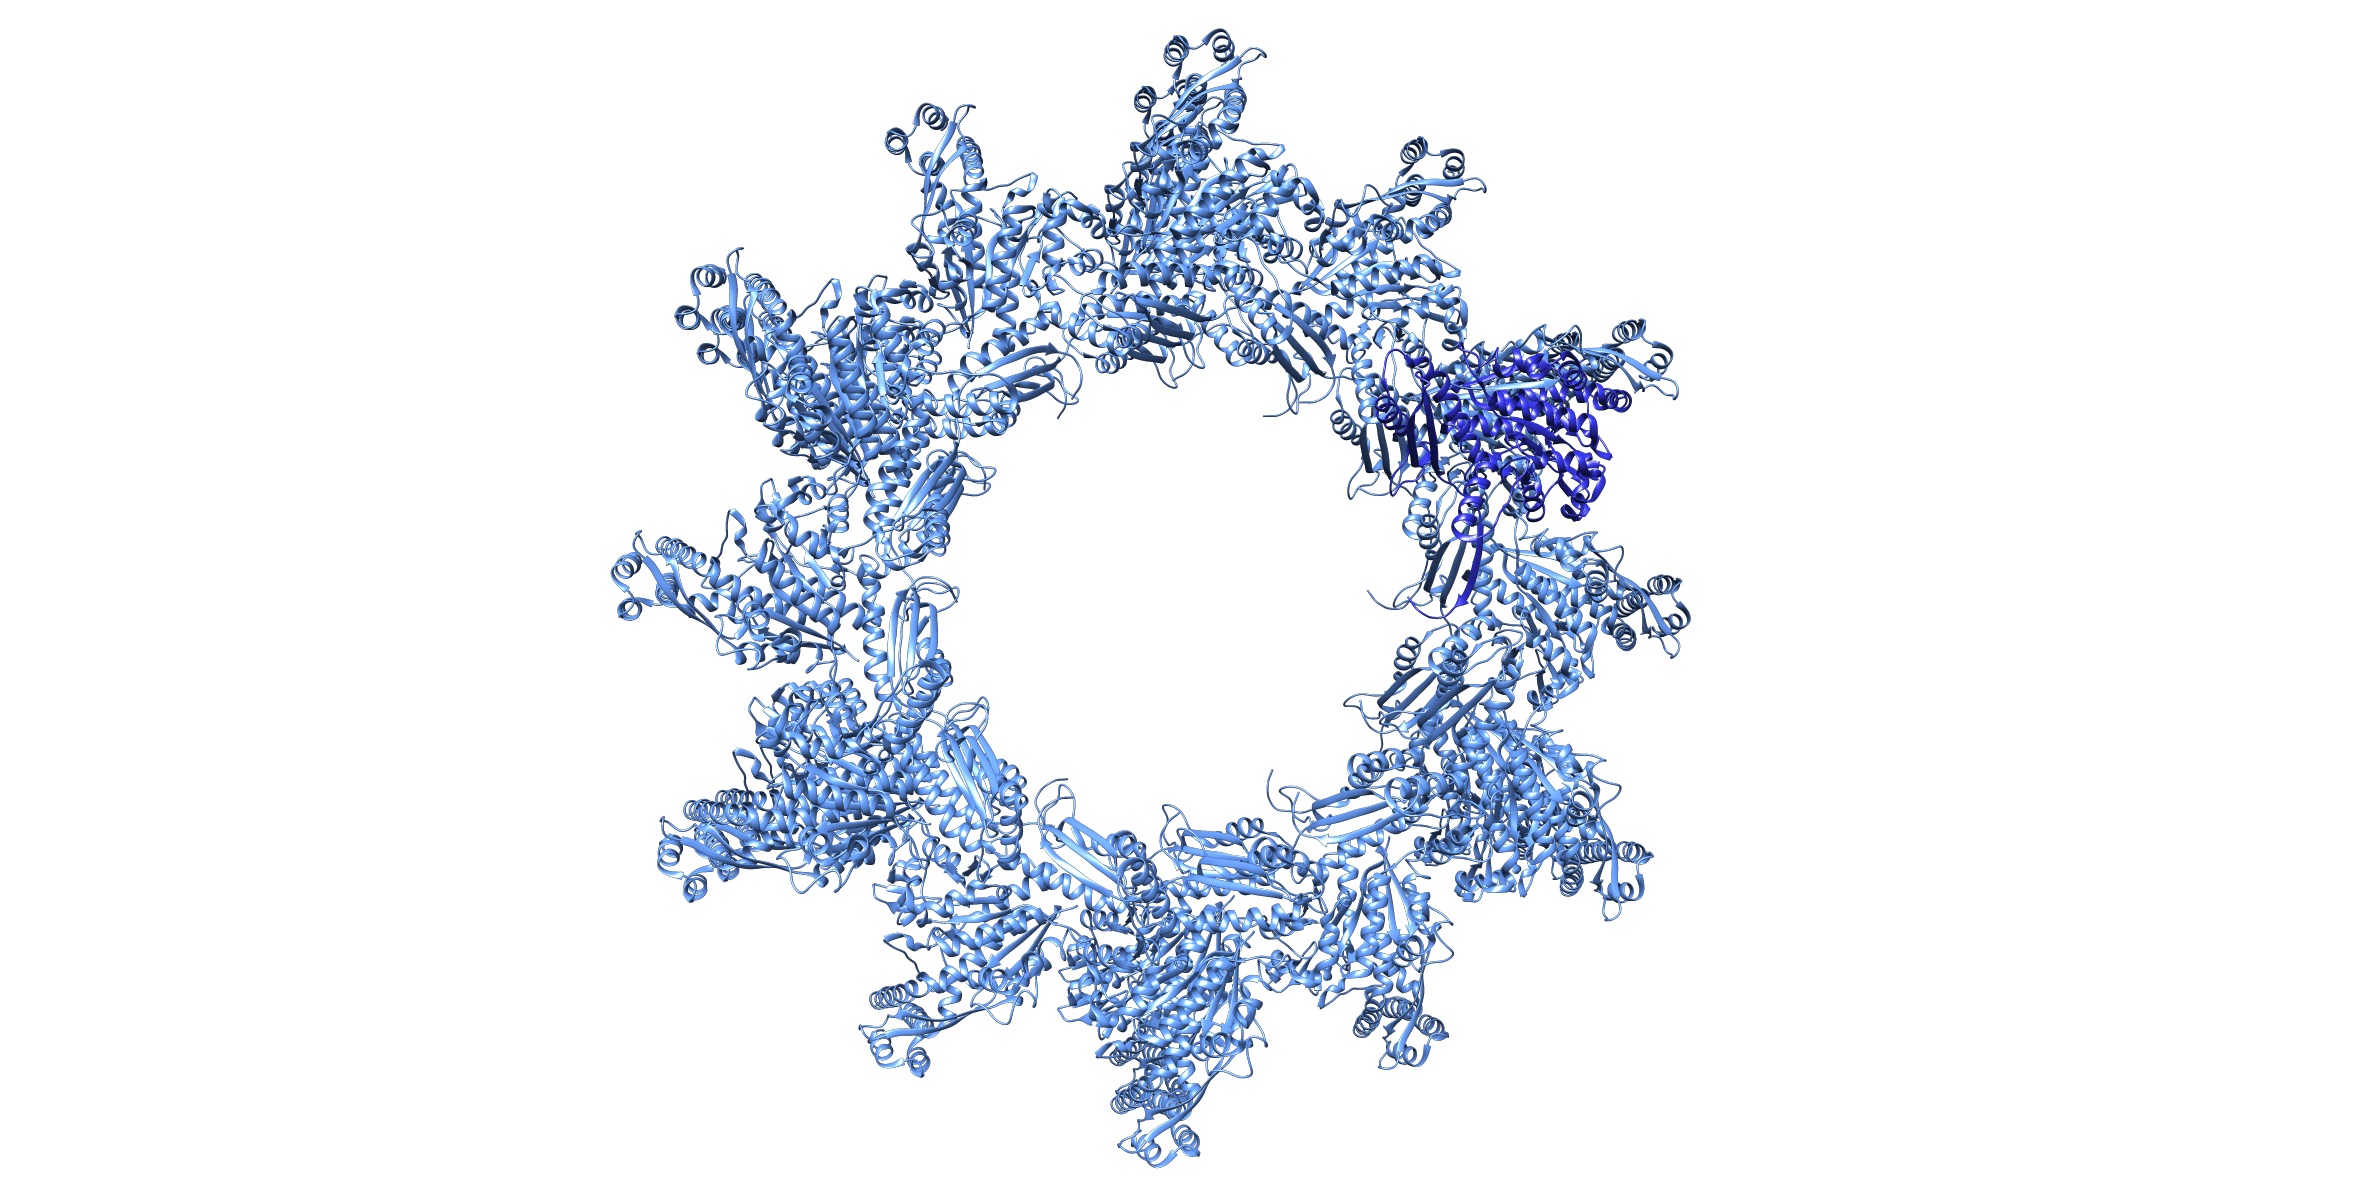
\includegraphics{img/schematics/9_7_1}

\href{http://rcsb.org/structure/5URX}{\emph{PDB: 5URX}}
A conformational change in the T6SS sheath provides the energy to fire the inner rod toward its target. The remaining sheath is shorter and wider than in its primed state, as in this section of a fired T6SS from \emph{Myxococcus xanthus} \citep{chang2017}.

\hypertarget{T6SS_battery}{%
\subsection*{More: T6SS battery}\label{T6SS_battery}}
\addcontentsline{toc}{subsection}{More: T6SS battery}

Some cells assemble a few, scattered type VI secretion systems. Other species, like this \emph{Amoebophilus asiaticus} build ordered arrays of parallel machines. These diderm bacteria live symbiotically inside amoebae. Their T6SS batteries help them colonize their host, perhaps by rupturing the membrane of the host phagosome that encloses them after they are engulfed, releasing them into the host cytoplasm. The number of T6SSs in each array varies, but can reach a few dozen.



\hypertarget{htmlwidget-4c250db5505e345e1849}{}

\label{fig:9-7a}\protect\hyperlink{tree}{Amoebophilus asiaticus} Collected by: \protect\hyperlink{martin_pilhofer}{Martin Pilhofer} Movie DOI: \href{https://doi.org/10.22002/D1.1583}{10.22002/D1.1583}

\hypertarget{MACs}{%
\subsection*{More: MACs}\label{MACs}}
\addcontentsline{toc}{subsection}{More: MACs}

\emph{Pseudoalteromonas luteoviolacea} produce massive arrays of MACs, contractile machines related to T6SSs. Cells lyse to release the arrays, like the one you see here, which can contain 100 individual MACs and extend more than 1 µm across. The arrays are highly ordered, with the tail fibers of the MACs networked into a hexagonal array that may help synchronize firing \protect\hyperlink{MAC_array_structure}{Schematic: MAC array structure}. MAC arrays serve an important function for larvae of the marine tubeworm \emph{Hydroides elegans}, and likely the larvae of other invertebrates such as sea urchins and corals as well. They signal to the larva that it is the right place to settle down and differentiate into a sessile (surface-attached) adult. The function of MAC arrays for the bacterium is less clear. It may be that the invertebrates benefit the lysed cell's surviving relatives in the biofilm. Or perhaps the MACs play another, completely unrelated role.

\emph{Note that this MAC array was produced by a cell lacking genes encoding other contractile weaponry (type VI secretion systems and bacteriocins). This was done to make it easier to identify the MACs.}



\hypertarget{htmlwidget-e9d9f06b3d7338b64e91}{}

\label{fig:9-7b}\protect\hyperlink{tree}{Pseudoalteromonas luteoviolacea} Collected by: \protect\hyperlink{martin_pilhofer}{Martin Pilhofer} Movie DOI: \href{https://doi.org/10.22002/D1.1584}{10.22002/D1.1584}

\hypertarget{MAC_array_structure}{%
\subsection*{Schematic: MAC array structure}\label{MAC_array_structure}}
\addcontentsline{toc}{subsection}{Schematic: MAC array structure}

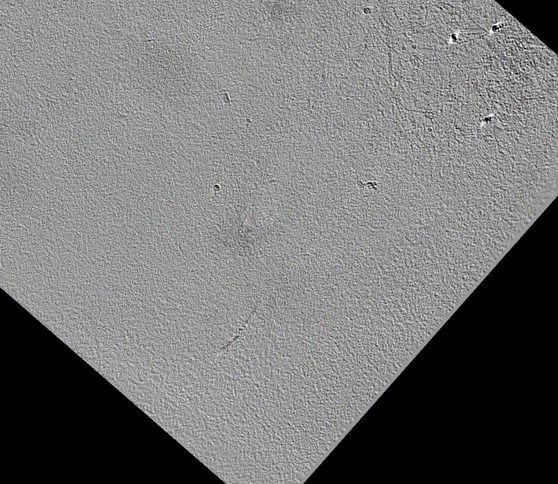
\includegraphics{img/schematics/9_7_2}

This digital segmentation of a MAC array shows the overall order of the structure \citep{shikuma2014}. Outer sheaths are in blue, inner rods in green, tail fibers in orange, and networking fibers in white.

\hypertarget{type-ix-secretion}{%
\section{Type IX Secretion}\label{type-ix-secretion}}

Instead of going to all the trouble of launching a weapon, why not just turn yourself into the weapon? \emph{Porphyromonas gingivalis} like this one use yet another secretion system, the type IX secretion system (T9SS), to secrete proteins called gingipains to the cell surface, where they are anchored to the outer membrane. Gingipains are peptidases, enzymes that chop up other proteins. In their lifestyle as human oral pathogens, the cells use gingipains to block host immune system signals and digest host biomolecules for food, causing the tissue damage of periodontitis.

In Chapter 6 you saw another T9SS with a very different function, in the gliding motility of \emph{Flavobacterium johnsoniae}. In that case, instead of gingipains, the machine secretes adhesive filaments which are also anchored to the cell surface.



\hypertarget{htmlwidget-2326f3b59ccd9d1326a6}{}

\label{fig:9-8}\protect\hyperlink{tree}{Porphyromonas gingivalis} Collected by: \protect\hyperlink{poorna_subramanian}{Poorna Subramanian} Movie DOI: \href{https://doi.org/10.22002/D1.1578}{10.22002/D1.1578}

\hypertarget{predation}{%
\section{Predation}\label{predation}}

Some bacteria take the strategy of eating the neighbors to a whole new level. Remember the pack-based hunting of \emph{Myxococcus xanthus} in Chapter 7 (chasing their prey with type IV pilus-based twitching motility)? There are also solitary hunters, like \emph{Bdellovibrio bacteriovorus}, which has evolved an elaborate vampiric lifestyle centered around its prey. You have already seen examples of \emph{B. bacteriovorus} cells on the prowl, in what is called ``attack phase.'' Their bodies are ideally shaped and sized for rapid flagellum-propelled swimming and all superfluous functions like growth and division are halted (remember the highly condensed nucleoid you saw at the end of Chapter 2). When a cell finds a diderm bacterium--\emph{Vibrio cholerae} in this case--it uses its type IV pili to lock on and pull itself closer, as you can see here.



\hypertarget{htmlwidget-8192a6f2dad05ade4bea}{}

\label{fig:9-9}\protect\hyperlink{tree}{Bdellovibrio bacteriovorus / Vibrio cholerae} Collected by: \protect\hyperlink{yi-wei_chang}{Yi-Wei Chang} Movie DOI: \href{https://doi.org/10.22002/D1.1579}{10.22002/D1.1579}

\hypertarget{predation-contd.}{%
\section{Predation (cont'd.)}\label{predation-contd.}}

Once a \emph{Bdellovibrio bacteriovorus} like this one has latched onto its unfortunate host, it opens a portal in the host's outer membrane, secreting a cocktail of enzymes that alter the host cell wall, causing the cell to round up and enlarge the periplasmic space. The \emph{B. bacteriovorus} quickly slides into the host periplasm through the portal \protect\hyperlink{Bdellovibrio_bacteriovorus_entry}{More: Bdellovibrio bacteriovorus entry} and seals the door behind it. In the process of preparing for entry, the cell dismantles equipment that is no longer necessary, including its chemosensory array and flagellum. As you can see here, the sheathed flagellum dislocates from the motor and is pulled into the periplasm, where the filament is degraded.

\emph{Note that the prey here--the small, round cell--comes from a mutant strain of} Escherichia coli \emph{that has an altered form of the shape-regulating protein MreB, which results in thinner cells. It is also lacking the Min system that positions the division plane at midcell. As a result, division occurs randomly along the length of the cell. The cells that divide near the pole produce ``minicells'' like this one. Minicells do not contain a genome and are not viable cells, but they can be useful for experiments. In this case, the reduced thickness of the sample improves the quality of cryoET imaging. It also lets us capture intermediates in the }B. bacteriovorus \emph{entry process \protect\hyperlink{Bdellovibrio_bacteriovorus_entry}{More: Bdellovibrio bacteriovorus entry}.}



\hypertarget{htmlwidget-dc3e5b141e1fca5bb500}{}

\label{fig:9-10}\protect\hyperlink{tree}{Bdellovibrio bacteriovorus / Escherichia coli} Collected by: \protect\hyperlink{yi-wei_chang}{Yi-Wei Chang} Movie DOI: \href{https://doi.org/10.22002/D1.1580}{10.22002/D1.1580}

\hypertarget{Bdellovibrio_bacteriovorus_entry}{%
\subsection*{More: Bdellovibrio bacteriovorus entry}\label{Bdellovibrio_bacteriovorus_entry}}
\addcontentsline{toc}{subsection}{More: Bdellovibrio bacteriovorus entry}

We still do not know exactly how \emph{Bdellovibrio bacteriovorus} enters its host, but the process is extremely rapid. In order to catch a snapshot, we mixed \emph{B. bacteriovorus} with miniaturized prey (see details above). As the \emph{B. bacteriovorus} cell cannot fit inside the prey, it remains stuck half-in and half-out. Note the tight collar of host outer membrane around the invader. How this seal is maintained throughout invasion remains a mystery.



\hypertarget{htmlwidget-4b8c098f7d3ec84bdc1f}{}

\label{fig:9-10a}\protect\hyperlink{tree}{Bdellovibrio bacteriovorus / Escherichia coli} Collected by: \protect\hyperlink{yi-wei_chang}{Yi-Wei Chang} Movie DOI: \href{https://doi.org/10.22002/D1.1585}{10.22002/D1.1585}

\hypertarget{predation-contd.-1}{%
\section{Predation (cont'd.)}\label{predation-contd.-1}}

Once inside its host, \emph{Bdellovibrio bacteriovorus} has the leisure to grow and replicate. From its position in the periplasm, the \emph{B. bacteriovorus} cell proceeds to digest the contents of the host cytoplasm, which shrinks down to a dense ball of (presumably undigestible) material. This meal provides the fuel necessary for the \emph{B. bacteriovorus} to grow to several times its original length and undergo a synchronous division to produce several (usually between 2 and 7) daughters. The number of progeny depends on the size of the host cell: two in the case of this relatively small \emph{Vibrio cholerae}. The progeny, reset to the attack phase (note the condensed nucleoids), finally lyse what is left of the host to escape and swim off in search of their next victims.



\hypertarget{htmlwidget-39c862c8d03a8d9b6b3a}{}

\label{fig:9-11}\protect\hyperlink{tree}{Bdellovibrio bacteriovorus / Vibrio cholerae} Collected by: \protect\hyperlink{yi-wei_chang}{Yi-Wei Chang} Movie DOI: \href{https://doi.org/10.22002/D1.1581}{10.22002/D1.1581}

\hypertarget{further-reading-8}{%
\section{Further Reading}\label{further-reading-8}}

Christie (2019). \emph{The rich tapestry of bacterial protein translocation systems} \citep{christie2019}.

Flemming et al. (2016). \emph{Biofilms: An emergent form of bacterial life} \citep{flemming2016}.

Patz et al. (2019). \emph{Phage tail-like particles are versatile bacterial nanomachines} \citep{patz2019}.

Sockett (2009). \emph{Predatory lifestyle of Bdellovibrio bacteriovorus} \citep{sockett2009}.

\hypertarget{viruses}{%
\chapter{Viruses}\label{viruses}}

\begin{quote}
``Phages are the winners in the game of life.''
- Forest Rohwer \citep{rohwer2014}
\end{quote}

\hypertarget{phage}{%
\section{Phage}\label{phage}}

Life is a battlefield for your cell, and other cells are not the only enemy. Attack can come from another front: viruses called phage (short for bacteriophage, or ``bacterium eaters'' because they were first identified infecting and killing bacteria). Like all viruses, phage use cells as vehicles for their replication. And, just like eukaryotic viruses, there is an army of different phage that prey on bacteria and archaea. No species is known to be immune.

The basic strategy of a phage is to inject its genome into a host cell, use the cell's machinery to replicate the genome and manufacture the proteins it encodes, then use these materials to build the next generation of phage. Since the phage is dependent on the cell's machinery for replication, it does not fulfill the criteria for a living organism. (Despite this distinction, we still talk about the viral ``lifecycle.'') By cleverly outsourcing, phage can be highly streamlined structurally, little more than a genome in an envelope en route to its next destination. All phage have a genome (either double or single-stranded DNA or RNA), tightly packed inside a protective envelope of either protein (forming a ``capsid'') or lipid, or both. The genome-containing shell is called the ``head'' of the phage. Many phage also have a tail, like this myophage attacking \emph{Shewanella oneidensis}. Fibers at the tip of the tail recognize features on their target host and allow the phage to dock.



\hypertarget{htmlwidget-702a1eb187a01a5aa785}{}

\label{fig:10-1}\protect\hyperlink{tree}{Shewanella oneidensis} Collected by: \protect\hyperlink{poorna_subramanian}{Poorna Subramanian} Movie DOI: \href{https://doi.org/10.22002/D1.1586}{10.22002/D1.1586}

\hypertarget{tails}{%
\section{Tails}\label{tails}}

Once docked, the phage delivers its cargo. The tails of some, but not all, phage are contractile, punching a channel through the cell's envelope to inject the genome, emptying the capsid as you see in this myophage infecting a \emph{Bacteroidetes} cell. This syringe-like mechanism should be familiar from the type VI secretion system and related weapons discussed in the last chapter. Evolution coopted phage tails for those structures, likely taking advantage of viral genes integrated into the genome of a bacterial host (more on that in a few pages).



\hypertarget{htmlwidget-eb706053f11d35d7c4dc}{}

\label{fig:10-2}\protect\hyperlink{tree}{Bacteroidetes JT5} Collected by: \protect\hyperlink{elitza_tocheva}{Elitza Tocheva} Movie DOI: \href{https://doi.org/10.22002/D1.1587}{10.22002/D1.1587}

\hypertarget{tails-contd.}{%
\section{Tails (cont'd.)}\label{tails-contd.}}

Some phage have tails that are not contractile, like this siphophage attacking a \emph{Shewanella oneidensis} cell. The long, flexible tail still serves the essential function of crossing the barrier of the cell's envelope, providing a conduit for the genome to enter the cell.

Note that we already saw a different type of phage attacking \emph{S. oneidensis}. While most phage are adapted to infect one or a few closely-related species of bacteria or archaea, there are often multiple different types of phage adapted to attack each species. The diversity of phage is staggering; one type lacks a single gene with detectable homology to any other in any known virus or cell.



\hypertarget{htmlwidget-698999dcd5776e135997}{}

\label{fig:10-3}\protect\hyperlink{tree}{Shewanella oneidensis} Collected by: \protect\hyperlink{poorna_subramanian}{Poorna Subramanian} Movie DOI: \href{https://doi.org/10.22002/D1.1588}{10.22002/D1.1588}

\hypertarget{variation-1}{%
\section{Variation}\label{variation-1}}

Not all phage tails are so long. Podophage (which this unidentified attacker of a \emph{Vibrio cholerae} may be) have short tails that extend after docking to cross the host envelope. Other phage lack tails entirely.

Similarly, heads can look very different. The unique rocket-ship shape of this phage's capsid highlights the diversity of phage morphology. Some, mostly infecting archaea in extreme environments, have heads shaped like bottles or lemons. Others take the form of long, thin filaments.



\hypertarget{htmlwidget-a841d2dfb9a64f2a35cb}{}

\label{fig:10-4}\protect\hyperlink{tree}{Vibrio cholerae} Collected by: \protect\hyperlink{yi-wei_chang}{Yi-Wei Chang} Movie DOI: \href{https://doi.org/10.22002/D1.1589}{10.22002/D1.1589}

\hypertarget{targeting}{%
\section{Targeting}\label{targeting}}

Unlike your cell, phage cannot direct their movement. They simply ride the currents of Brownian motion, waiting to bump into a target receptor they can latch onto. Their abundance helps; in the ocean, there are about ten times as many phage as bacteria. Still, it might be a long wait, so evolution has fashioned some mechanisms to speed things up. One strategy is to target a receptor not on the cell body itself, but on a long, more easily-encountered cell appendage.

Some species of bacteria, including this \emph{Escherichia coli} use ``competence pili'' assembled by a Type IV Secretion System to take up DNA from other cells. This ``horizontal gene transfer'' (in contrast to ``vertical'' heredity from mother to daughter) lets asexually-reproducing cells mix and match genes to potential advantage. It also blurs the line between species (more about that in the \protect\hyperlink{tree}{Phylogenetic Tree}). And in this case, it offers an advantage to these MS2 leviphage, which have evolved to recognize the pilus and inject their own RNA into the nucleic acid uptake channel.



\hypertarget{htmlwidget-230bb6b16bac85993164}{}

\label{fig:10-5}\protect\hyperlink{tree}{Escherichia coli} Collected by: \protect\hyperlink{yi-wei_chang}{Yi-Wei Chang} Movie DOI: \href{https://doi.org/10.22002/D1.1590}{10.22002/D1.1590}

\hypertarget{targeting-contd.}{%
\section{Targeting (cont'd.)}\label{targeting-contd.}}

Other phage use bacterial appendages in an even cleverer way. These φCb13 myophage take advantage of the cell's motility to hitch a ride to the cell. They have a filament on their head that wraps into the helical groove of the \emph{Caulobacter crescentus} flagellum. Remember that flagella can spin either clockwise or counter-clockwise. If this single polar flagellum spins clockwise, pushing the cell body, the attached phage would unscrew like a nut off the end of the flagellum. But if the flagellum spins counter-clockwise, the nut will instead spin down to the cell body, where its tail fibers will find their receptors and its tail will inject the genome \protect\hyperlink{ux3c6Cb13_infection}{More: φCb13 infection}.



\hypertarget{htmlwidget-2ee09562bdb0a61cdf98}{}

\label{fig:10-6}\protect\hyperlink{tree}{Caulobacter crescentus} Collected by: \protect\hyperlink{elizabeth_wright}{Elizabeth Wright} Movie DOI: \href{https://doi.org/10.22002/D1.1591}{10.22002/D1.1591}

\hypertarget{ux3c6Cb13_infection}{%
\subsection*{More: φCb13 infection}\label{ux3c6Cb13_infection}}
\addcontentsline{toc}{subsection}{More: φCb13 infection}

Here you see several φCb13 phage that have successfully reached their target receptors at the pole of a \emph{Caulobacter crescentus} and are in the process of infecting the cell (note the mix of filled capsids that have not yet released their genome and empty capsids that have).



\hypertarget{htmlwidget-07a4b8280d02356217d8}{}

\label{fig:10-6a}\protect\hyperlink{tree}{Caulobacter crescentus} Collected by: \protect\hyperlink{elizabeth_wright}{Elizabeth Wright} Movie DOI: \href{https://doi.org/10.22002/D1.1596}{10.22002/D1.1596}

\hypertarget{replication}{%
\section{Replication}\label{replication}}

Once inside a cell, phage adopt one of two strategies. The first is to go through a straightforward round of replication, using their host's machinery. The second is to stick around a while. To do that, the phage inserts its genome into that of its host, creating an addition called a ``prophage'' that will be propagated indefinitely through cell replication. At some point in the future, usually in response to a stress that threatens the host, the prophage uses special DNA sequences at its ends akin to an ejection seat to pop its genes back out of the host genome, and carry out a normal viral replication and release cycle. Prophage are not simply passengers, though. Some confer a beneficial function on the host; a filamentous inophage carries the disease-causing ``cholera toxin'' in the \emph{Vibrio cholerae} genome. Prophage also offer a source of genetic diversity to their host. Mutations sometimes alter the ejection sequences, rendering a prophage a permanent part of the genome, or genetic recombination may shuffle some or part of the prophage into a different part of the genome. Further evolution may then put these pieces to new use. This is likely how bacteria got the contractile weapons you saw in the last chapter, repurposing genes encoding phage tail components.

Whether the phage replicates immediately or waits a while as a prophage first, the cycle of replication and release is rapid. The virus hijacks the cell's protein-making machinery to churn out packaging proteins like capsid, and its replication machinery to churn out copies of the genome. Genomes are quickly (and very densely) packed into new heads, tails attached if necessary, and the mature phage released. Not all phage lyse their hosts; some filamentous phage (which are commonly beneficial) use secretion machinery to exit without harm. Most, though, use proteins that self-assemble into ports in the inner membrane, allowing another phage-encoded protein to access and chew up the cell wall, causing the cell to lyse. Here you can see a snapshot of this process in a \emph{Vibrio cholerae} cell infected by a phage that is not its virulence-enhancing friend. The phage is replicating, and has just lysed the cell to make its escape.



\hypertarget{htmlwidget-2d8cb0435b5934f5521a}{}

\label{fig:10-7}\protect\hyperlink{tree}{Vibrio cholerae} Collected by: \protect\hyperlink{poorna_subramanian}{Poorna Subramanian} Movie DOI: \href{https://doi.org/10.22002/D1.1592}{10.22002/D1.1592}

\hypertarget{release}{%
\section{Release}\label{release}}

Some archaeal phage make an even more dramatic exit, through virus-associated pyramids, or VAPs. You can see these escape hatches in this \emph{Sulfolobus solfataricus} cell infected with \emph{Sulfolobus} Turreted Icosahedral Virus (STIV) \protect\hyperlink{STIV_structure}{Schematic: STIV structure}. The VAPs are made from a single phage-encoded protein that self-assembles into a seven-sided pyramid in the membrane. Note how the VAPs poke through and disrupt the cell's surface layer. Note also the many, many copies the phage has made. We sometimes see storage granules inside VAPs, likely simply pushed there by excluding forces from the densely-packed nucleoid and assembling viral capsids in the center of the cell.



\hypertarget{htmlwidget-5848aa254035fed53c1a}{}

\label{fig:10-8}\protect\hyperlink{tree}{Sulfolobus solfataricus} Collected by: \protect\hyperlink{lu_gan}{Lu Gan} Movie DOI: \href{https://doi.org/10.22002/D1.1593}{10.22002/D1.1593}

\hypertarget{STIV_structure}{%
\subsection*{Schematic: STIV structure}\label{STIV_structure}}
\addcontentsline{toc}{subsection}{Schematic: STIV structure}

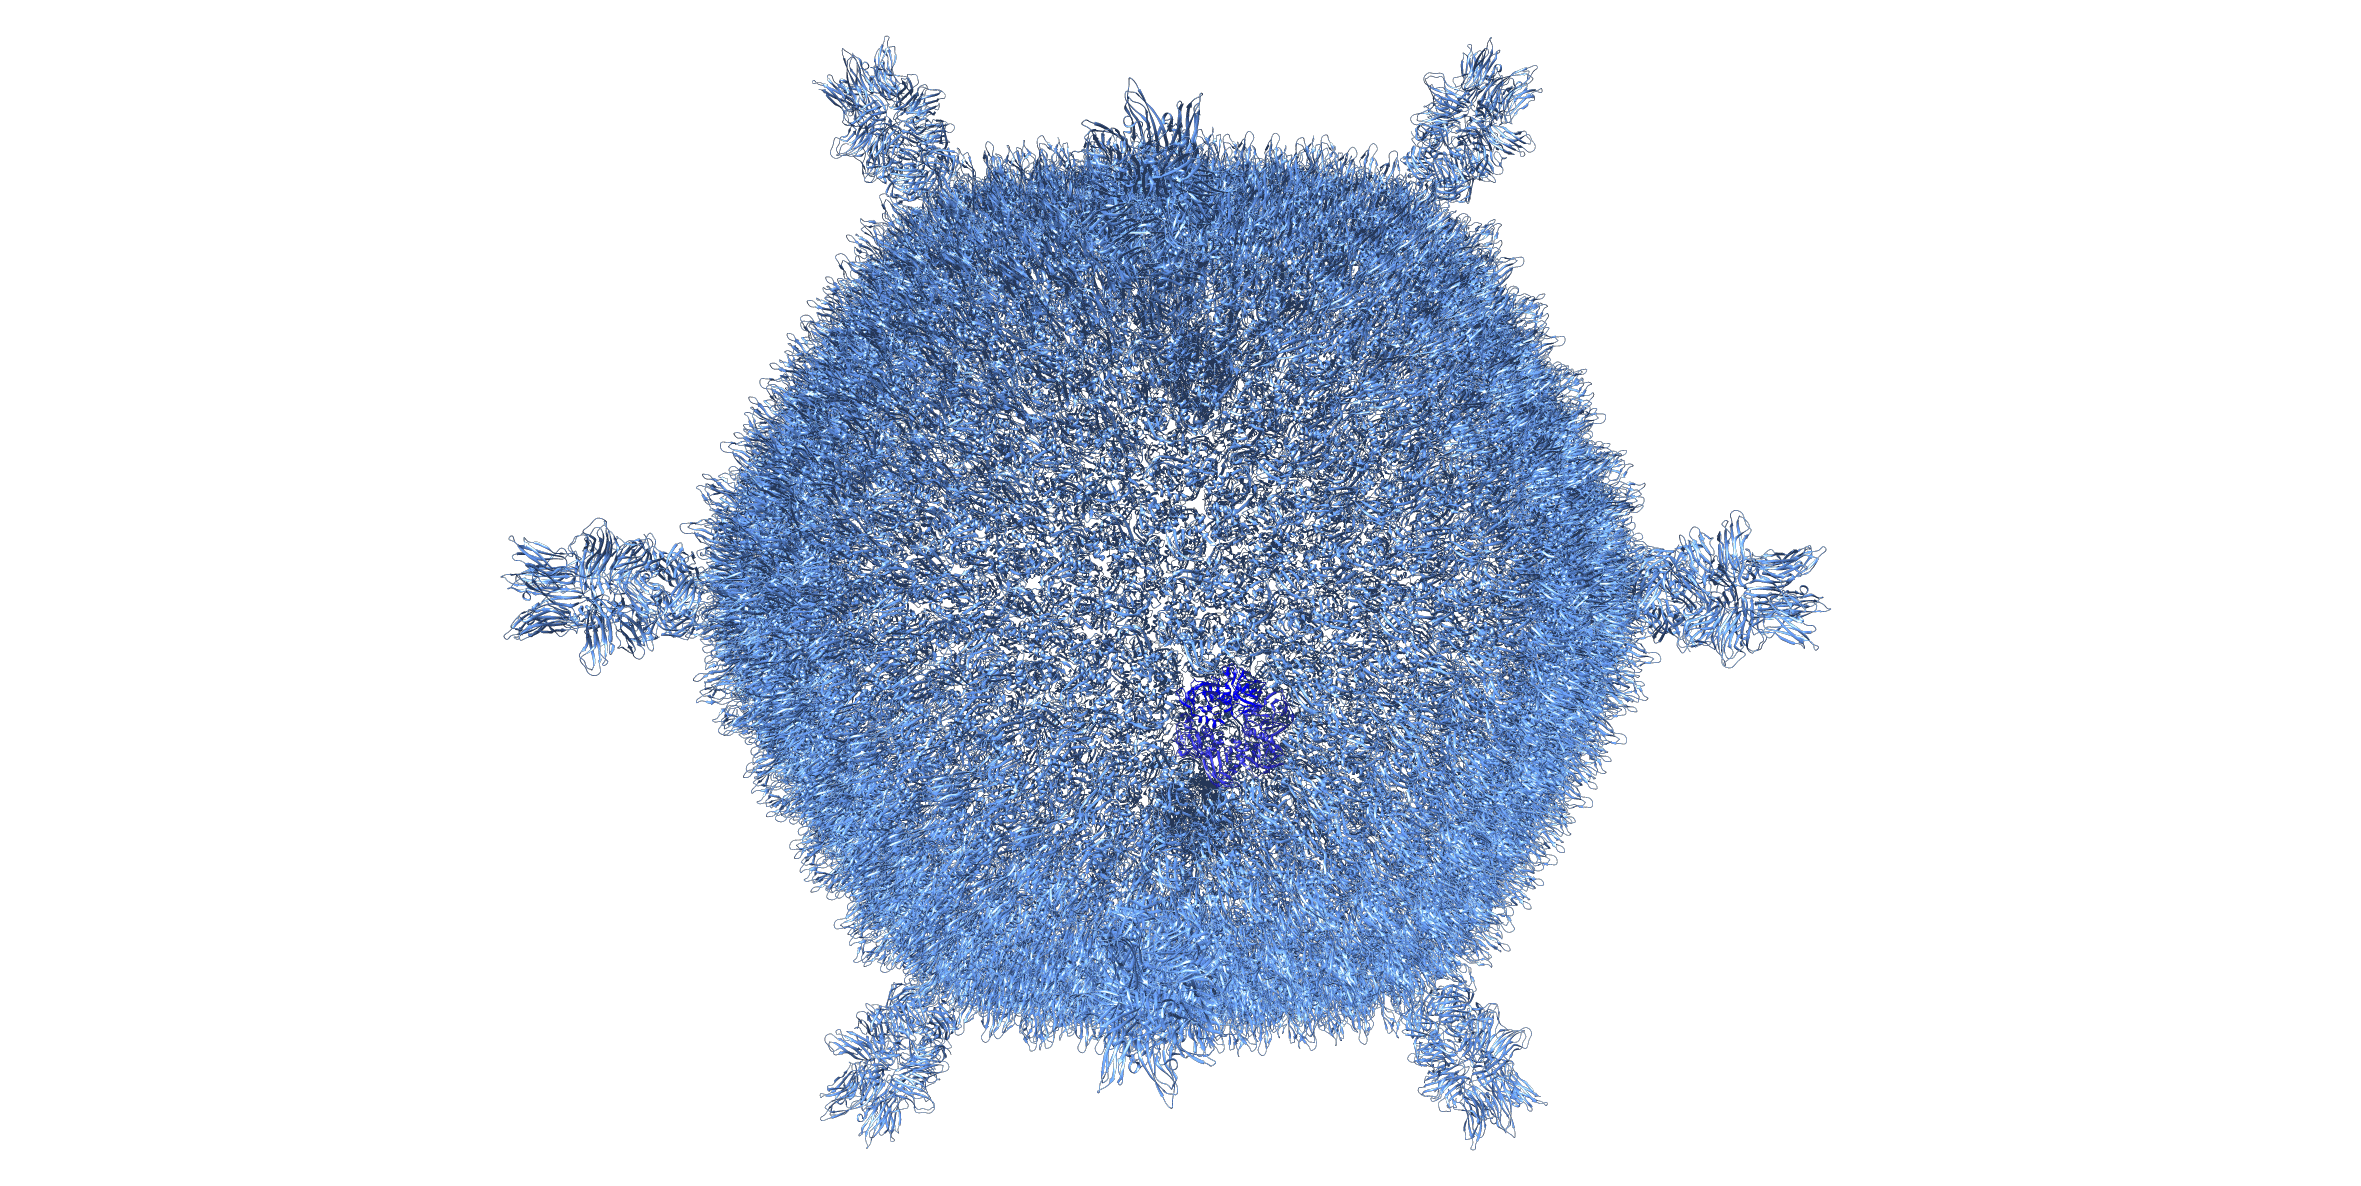
\includegraphics{img/schematics/10_8_1}

\href{http://rcsb.org/structure/3J31}{\emph{PDB: 3J31}}
As their name implies, STIV have icosahedral capsids with protruding turrets. The hexameric repeating unit in the shell is formed by three copies of a double-lobed protein, as you can see in this structure \citep{veesler2013}.

\hypertarget{release-contd.}{%
\section{Release (cont'd.)}\label{release-contd.}}

When the STIV phage is ready to make its great escape, a still-unknown signal triggers the pyramids to open along their seams, peeling back to create 100 nm-wide holes for the phage, and all the other contents of the cell, to pour out, as you can see in this lysed \emph{Sulfolobus solfataricus} cell infected with the same virus.



\hypertarget{htmlwidget-453691e2402f8c1d81f8}{}

\label{fig:10-9}\protect\hyperlink{tree}{Sulfolobus solfataricus} Collected by: \protect\hyperlink{lu_gan}{Lu Gan} Movie DOI: \href{https://doi.org/10.22002/D1.1594}{10.22002/D1.1594}

\hypertarget{cellular-defense}{%
\section{Cellular Defense}\label{cellular-defense}}

So what can your cell do to protect itself from these attackers? The most well-known defense is the CRISPR-Cas system now widely used to edit genomes across the tree of life. Its original function, though, is as an immune system similar to our own. Bacterial and archaeal cells ``record'' snippets of the genes of infecting phage in their own genome, enabling the cell to rapidly identify and chop up matching genes in future infections, much as our immune system stores the memory of antigen fragments for rapid neutralization in the future.

Defense can also be structural. Surface layers may protect cells from some phage. And then there is always distraction. One function of extracellular vesicles may be to provide decoys for phage to attack, as you can see with this myophage attacking a \emph{Shewanella oneidensis} outer membrane vesicle. The war between cells and viruses is an ancient one, and continually raging. Despite your cell's best efforts, it is very likely that it will end its life in a burst of phage. It is far from alone in this fate, though. In the ocean off Florida, it has been estimated that every day phage kill off half the bacterial population. But each lysed cell provides a feast for a starving neighbor, and DNA for more evolutionary tinkering, continuing to shape the weird, wonderful microbial world.



\hypertarget{htmlwidget-2a6705e046271bb3f67d}{}

\label{fig:10-10}\protect\hyperlink{tree}{Shewanella oneidensis} Collected by: \protect\hyperlink{lauren_ann_metskas}{Lauren Ann Metskas} Movie DOI: \href{https://doi.org/10.22002/D1.1595}{10.22002/D1.1595}

\hypertarget{further-reading-9}{%
\section{Further Reading}\label{further-reading-9}}

Keen (2015). \emph{A century of phage research: Bacteriophages and the shaping of modern biology} \citep{keen2015}.

Prangishvili et al. (2017). \emph{The enigmatic archaeal virosphere} \citep{prangishvili2017}.

Rohwer et al. (2014). \emph{Life in Our Phage World} \citep{rohwer2014}.

\hypertarget{appendix-appendix}{%
\appendix}


\hypertarget{feature-index}{%
\chapter{Feature Index}\label{feature-index}}

Click on a feature in the sidebar to see examples in different species.

\hypertarget{adhe-spirosomes}{%
\section*{AdhE spirosomes}\label{adhe-spirosomes}}
\addcontentsline{toc}{section}{AdhE spirosomes}

Clostridium thermocellum \ref{fig:4-5}

\hypertarget{adhesion-complexes-and-filaments}{%
\section*{Adhesion complexes and filaments}\label{adhesion-complexes-and-filaments}}
\addcontentsline{toc}{section}{Adhesion complexes and filaments}

Flavobacterium johnsoniae \ref{fig:6-11}

Mycoplasma genitalium \ref{fig:2-1}

Mycoplasma pneumoniae \ref{fig:6-12}

\hypertarget{archaella}{%
\section*{Archaella}\label{archaella}}
\addcontentsline{toc}{section}{Archaella}

Halobacterium salinarum \ref{fig:3-7a}

Halobacterium salinarum \ref{fig:6-9c}

Haloferax gibbonsii \ref{fig:4-10a}

Halohasta litchfieldiae \ref{fig:4-10b}

Halorubrum litoreum \ref{fig:4-10}

Methanobacterium formicicum \ref{fig:2-7d}

Methanoregula formicica \ref{fig:6-8}

Methanoregula formicica \ref{fig:3-2b}

Methanospirillum hungatei \ref{fig:2-8}

Methanospirillum hungatei \ref{fig:7-3}

Sulfolobus acidocaldarius \ref{fig:5-11}

Sulfolobus acidocaldarius \ref{fig:5-12}

Thermococcus kodakaraensis \ref{fig:6-9}

Thermococcus kodakaraensis \ref{fig:6-9a}

Thermococcus kodakaraensis \ref{fig:6-9b}

\hypertarget{archaellar-cone}{%
\section*{Archaellar cone}\label{archaellar-cone}}
\addcontentsline{toc}{section}{Archaellar cone}

Thermococcus kodakaraensis \ref{fig:6-9}

Thermococcus kodakaraensis \ref{fig:6-9a}

Thermococcus kodakaraensis \ref{fig:6-9b}

Thermococcus kodakaraensis \ref{fig:8-3}

\hypertarget{carboxysomes-1}{%
\section*{Carboxysomes}\label{carboxysomes-1}}
\addcontentsline{toc}{section}{Carboxysomes}

Halothiobacillus neapolitanus \ref{fig:4-7a}

Halothiobacillus neapolitanus \ref{fig:4-9b}

Hydrogenovibrio crunogenus \ref{fig:4-7b}

Hydrogenovibrio crunogenus \ref{fig:4-9a}

Thiomonas intermedia \ref{fig:4-7}

Thiomonas intermedia \ref{fig:5-1}

\hypertarget{cdv-belt}{%
\section*{Cdv belt}\label{cdv-belt}}
\addcontentsline{toc}{section}{Cdv belt}

Sulfolobus acidocaldarius \ref{fig:5-11}

Sulfolobus acidocaldarius \ref{fig:5-12}

\hypertarget{cell-wall-diderm}{%
\section*{Cell wall (diderm)}\label{cell-wall-diderm}}
\addcontentsline{toc}{section}{Cell wall (diderm)}

Acetonema longum \ref{fig:4-6}

Acetonema longum \ref{fig:4-6}

Acetonema longum \ref{fig:8-10}

Acetonema longum \ref{fig:8-10a}

Acetonema longum \ref{fig:8-11}

Acetonema longum \ref{fig:8-9}

Agrobacterium tumefaciens \ref{fig:4-9}

Agrobacterium tumefaciens \ref{fig:5-8}

Agrobacterium tumefaciens \ref{fig:9-1}

Amoebophilus asiaticus \ref{fig:9-7a}

Azospirillum brasilense \ref{fig:7-4a}

Bacteroidetes JT5 \ref{fig:10-2}

Bdellovibrio bacteriovorus \ref{fig:2-10}

Bdellovibrio bacteriovorus \ref{fig:6-2}

Bdellovibrio bacteriovorus \ref{fig:6-2a}

Bdellovibrio bacteriovorus \ref{fig:9-10}

Bdellovibrio bacteriovorus \ref{fig:9-10a}

Bdellovibrio bacteriovorus \ref{fig:9-11}

Bdellovibrio bacteriovorus \ref{fig:9-9}

Borrelia burgdorferi \ref{fig:2-4a}

Borrelia burgdorferi \ref{fig:2-4b}

Borrelia burgdorferi \ref{fig:3-5a}

Borrelia burgdorferi \ref{fig:6-7}

Brucella abortus \ref{fig:3-2a}

Campylobacter jejuni \ref{fig:3-5}

Campylobacter jejuni \ref{fig:6-4}

Caulobacter crescentus \ref{fig:2-6}

Caulobacter crescentus \ref{fig:3-4}

Caulobacter crescentus \ref{fig:4-1}

Caulobacter crescentus \ref{fig:5-10}

Caulobacter crescentus \ref{fig:5-2}

Caulobacter crescentus \ref{fig:5-7}

Caulobacter crescentus \ref{fig:5-7a}

Caulobacter crescentus \ref{fig:10-6}

Caulobacter crescentus \ref{fig:10-6a}

Caulobacter crescentus \ref{fig:8-1}

Caulobacter crescentus \ref{fig:8-4}

Chloroflexi \ref{fig:4-4}

Chloroflexi \ref{fig:5-6b}

Cupriavidus necator \ref{fig:4-8}

Cupriavidus necator \ref{fig:5-9}

Cupriavidus necator \ref{fig:5-9a}

Cupriavidus necator \ref{fig:3-2}

Delftia acidovorans \ref{fig:2-6a}

Escherichia coli \ref{fig:2-3a}

Escherichia coli \ref{fig:10-5}

Escherichia coli \ref{fig:9-5}

Flavobacterium johnsoniae \ref{fig:6-11}

Gluconacetobacter hansenii \ref{fig:9-2}

Halothiobacillus neapolitanus \ref{fig:4-7a}

Halothiobacillus neapolitanus \ref{fig:4-9b}

Helicobacter hepaticus \ref{fig:6-6}

Helicobacter pylori \ref{fig:6-4a}

Helicobacter pylori \ref{fig:8-2}

Helicobacter pylori \ref{fig:9-3a}

Hydrogenovibrio crunogenus \ref{fig:2-3}

Hydrogenovibrio crunogenus \ref{fig:4-7b}

Hydrogenovibrio crunogenus \ref{fig:4-9a}

Hylemonella gracilis \ref{fig:3-3}

Hylemonella gracilis \ref{fig:6-3}

Hyphomonas neptunium \ref{fig:5-3}

Hyphomonas neptunium \ref{fig:5-3a}

Hyphomonas neptunium \ref{fig:5-3b}

Idiomarina loihiensis \ref{fig:5-6}

Legionella pneumophila \ref{fig:9-3}

Lysobacter antibioticus \ref{fig:4-8a}

Magnetospirillum magneticum \ref{fig:7-6}

Methylomicrobium alcaliphilum \ref{fig:2-7a}

Methyloprofundus sedimenti \ref{fig:4-3a}

Mycobacterium marinum \ref{fig:2-5}

Myxococcus xanthus \ref{fig:2-4}

Myxococcus xanthus \ref{fig:2-4c}

Myxococcus xanthus \ref{fig:6-10}

Myxococcus xanthus \ref{fig:9-6}

Porphyromonas gingivalis \ref{fig:9-8}

Prosthecobacter debontii \ref{fig:2-4d}

Prosthecobacter vanneervenii \ref{fig:3-6a}

Prosthecobacter vanneervenii \ref{fig:8-4a}

Proteus mirabilis \ref{fig:6-5a}

Pseudomonas aeruginosa \ref{fig:6-3a}

Pseudomonas aeruginosa \ref{fig:9-4}

Pseudomonas flexibilis \ref{fig:6-5}

Rhodopseudomonas palustris \ref{fig:4-3}

Salmonella typhimurium \ref{fig:7-2}

Shewanella oneidensis \ref{fig:4-2}

Shewanella oneidensis \ref{fig:10-1}

Shewanella oneidensis \ref{fig:10-3}

Shewanella oneidensis \ref{fig:7-1}

Sphingopyxis alaskensis \ref{fig:5-6a}

Sporomusa acidovorans \ref{fig:8-10c}

Thiomonas intermedia \ref{fig:5-1}

Treponema primitia \ref{fig:6-7a}

Verrucomicrobium spinosum \ref{fig:3-6}

Vibrio cholerae \ref{fig:10-4}

Vibrio cholerae \ref{fig:10-7}

Vibrio cholerae \ref{fig:7-4}

Vibrio cholerae \ref{fig:7-5a}

Vibrio cholerae \ref{fig:9-7}

\hypertarget{cell-wall-monoderm}{%
\section*{Cell wall (monoderm)}\label{cell-wall-monoderm}}
\addcontentsline{toc}{section}{Cell wall (monoderm)}

Bacillus subtilis \ref{fig:2-2a}

Bacillus subtilis \ref{fig:8-5}

Bacillus subtilis \ref{fig:8-5a}

Bacillus subtilis \ref{fig:8-6}

Bacillus subtilis \ref{fig:8-6a}

Bacillus subtilis \ref{fig:8-6b}

Clostridium thermocellum \ref{fig:2-7b}

Clostridium thermocellum \ref{fig:4-5}

Listeria monocytogenes \ref{fig:2-2}

Methanobacterium formicicum \ref{fig:2-2c}

Staphylococcus aureus \ref{fig:5-4}

Tetrasphaera remsis \ref{fig:5-5}

\hypertarget{cellulose}{%
\section*{Cellulose}\label{cellulose}}
\addcontentsline{toc}{section}{Cellulose}

Agrobacterium tumefaciens \ref{fig:9-1}

Gluconacetobacter hansenii \ref{fig:9-2}

\hypertarget{chemosensory-arrays-membrane-bound}{%
\section*{Chemosensory arrays (membrane-bound)}\label{chemosensory-arrays-membrane-bound}}
\addcontentsline{toc}{section}{Chemosensory arrays (membrane-bound)}

Acetonema longum \ref{fig:4-6}

Acetonema longum \ref{fig:8-9}

Azospirillum brasilense \ref{fig:7-4a}

Bacillus subtilis \ref{fig:8-5}

Bdellovibrio bacteriovorus \ref{fig:2-10}

Bdellovibrio bacteriovorus \ref{fig:6-2}

Bdellovibrio bacteriovorus \ref{fig:9-10}

Bdellovibrio bacteriovorus \ref{fig:9-9}

Campylobacter jejuni \ref{fig:3-5}

Campylobacter jejuni \ref{fig:6-4}

Caulobacter crescentus \ref{fig:10-6}

Caulobacter crescentus \ref{fig:2-6}

Caulobacter crescentus \ref{fig:8-4}

Cupriavidus necator \ref{fig:5-9}

Helicobacter hepaticus \ref{fig:6-6}

Helicobacter pylori \ref{fig:6-4a}

Helicobacter pylori \ref{fig:8-2}

Helicobacter pylori \ref{fig:9-3a}

Hydrogenovibrio crunogenus \ref{fig:4-7b}

Hydrogenovibrio crunogenus \ref{fig:4-9a}

Hylemonella gracilis \ref{fig:3-3}

Hylemonella gracilis \ref{fig:6-3}

Magnetospirillum magneticum \ref{fig:7-6}

Methanoregula formicica \ref{fig:3-2b}

Methanospirillum hungatei \ref{fig:2-8}

Methanospirillum hungatei \ref{fig:7-3}

Proteus mirabilis \ref{fig:6-5a}

Pseudomonas aeruginosa \ref{fig:6-3a}

Salmonella typhimurium \ref{fig:7-2}

Shewanella oneidensis \ref{fig:10-1}

Shewanella oneidensis \ref{fig:4-2}

Shewanella oneidensis \ref{fig:7-1}

Thermococcus kodakaraensis \ref{fig:6-9a}

Thermococcus kodakaraensis \ref{fig:6-9b}

Treponema primitia \ref{fig:6-7a}

Vibrio cholerae \ref{fig:10-4}

Vibrio cholerae \ref{fig:10-7}

Vibrio cholerae \ref{fig:7-4}

Vibrio cholerae \ref{fig:7-5a}

Vibrio cholerae \ref{fig:9-7}

\hypertarget{chemosensory-arrays-cytoplasmic}{%
\section*{Chemosensory arrays (cytoplasmic)}\label{chemosensory-arrays-cytoplasmic}}
\addcontentsline{toc}{section}{Chemosensory arrays (cytoplasmic)}

Methanoregula formicica \ref{fig:3-2b}

Methanoregula formicica \ref{fig:7-5}

Vibrio cholerae \ref{fig:7-5a}

\hypertarget{chlorosomes}{%
\section*{Chlorosomes}\label{chlorosomes}}
\addcontentsline{toc}{section}{Chlorosomes}

Chloroflexi \ref{fig:4-4}

\hypertarget{ctp-synthase-filaments}{%
\section*{CTP synthase filaments}\label{ctp-synthase-filaments}}
\addcontentsline{toc}{section}{CTP synthase filaments}

Caulobacter crescentus \ref{fig:3-4}

\hypertarget{division-plane}{%
\section*{Division plane}\label{division-plane}}
\addcontentsline{toc}{section}{Division plane}

Agrobacterium tumefaciens \ref{fig:5-8}

Caulobacter crescentus \ref{fig:4-1}

Caulobacter crescentus \ref{fig:5-10}

Caulobacter crescentus \ref{fig:5-2}

Caulobacter crescentus \ref{fig:8-4}

Cupriavidus necator \ref{fig:3-2}

Cupriavidus necator \ref{fig:4-8}

Cupriavidus necator \ref{fig:5-9}

Cupriavidus necator \ref{fig:5-9a}

Halohasta litchfieldiae \ref{fig:4-10b}

Listeria monocytogenes \ref{fig:2-2}

Porphyromonas gingivalis \ref{fig:9-8}

Sphingopyxis alaskensis \ref{fig:5-6a}

Staphylococcus aureus \ref{fig:5-4}

Sulfolobus acidocaldarius \ref{fig:5-11}

Sulfolobus acidocaldarius \ref{fig:5-12}

Thiomonas intermedia \ref{fig:5-1}

\hypertarget{division-septum}{%
\section*{Division septum}\label{division-septum}}
\addcontentsline{toc}{section}{Division septum}

Tetrasphaera remsis \ref{fig:5-5}

\hypertarget{dna-1}{%
\section*{DNA}\label{dna-1}}
\addcontentsline{toc}{section}{DNA}

Haloarcula argentinensis \ref{fig:2-9}

Hyphomonas neptunium \ref{fig:5-3}

Vibrio cholerae \ref{fig:10-7}

\hypertarget{flagella-external-unsheathed}{%
\section*{Flagella (external, unsheathed)}\label{flagella-external-unsheathed}}
\addcontentsline{toc}{section}{Flagella (external, unsheathed)}

Acetonema longum \ref{fig:4-6}

Acetonema longum \ref{fig:8-9}

Agrobacterium tumefaciens \ref{fig:9-1}

Amoebophilus asiaticus \ref{fig:9-7a}

Azospirillum brasilense \ref{fig:7-4a}

Bacillus subtilis \ref{fig:8-6a}

Campylobacter jejuni \ref{fig:3-5}

Campylobacter jejuni \ref{fig:6-1}

Campylobacter jejuni \ref{fig:6-4}

Caulobacter crescentus \ref{fig:10-6}

Caulobacter crescentus \ref{fig:5-7}

Caulobacter crescentus \ref{fig:8-1}

Caulobacter crescentus \ref{fig:8-4}

Escherichia coli \ref{fig:9-10a}

Helicobacter pylori \ref{fig:6-4a}

Hydrogenovibrio crunogenus \ref{fig:2-3}

Hylemonella gracilis \ref{fig:3-3}

Hylemonella gracilis \ref{fig:6-3}

Hyphomonas neptunium \ref{fig:5-3b}

Listeria monocytogenes \ref{fig:2-2}

Methylomicrobium alcaliphilum \ref{fig:2-7a}

Proteus mirabilis \ref{fig:6-5a}

Pseudomonas flexibilis \ref{fig:6-5}

Salmonella typhimurium \ref{fig:7-2}

Shewanella oneidensis \ref{fig:10-1}

Shewanella oneidensis \ref{fig:10-10}

Shewanella oneidensis \ref{fig:4-2}

Shewanella oneidensis \ref{fig:7-1}

Sporomusa acidovorans \ref{fig:8-10c}

\hypertarget{flagella-periplasmic}{%
\section*{Flagella (periplasmic)}\label{flagella-periplasmic}}
\addcontentsline{toc}{section}{Flagella (periplasmic)}

Borrelia burgdorferi \ref{fig:2-4a}

Borrelia burgdorferi \ref{fig:2-4b}

Borrelia burgdorferi \ref{fig:3-5a}

Borrelia burgdorferi \ref{fig:6-7}

Treponema primitia \ref{fig:6-7a}

\hypertarget{flagella-sheathed}{%
\section*{Flagella (sheathed)}\label{flagella-sheathed}}
\addcontentsline{toc}{section}{Flagella (sheathed)}

Bdellovibrio bacteriovorus \ref{fig:2-10}

Bdellovibrio bacteriovorus \ref{fig:6-2}

Bdellovibrio bacteriovorus \ref{fig:9-10}

Helicobacter hepaticus \ref{fig:6-6}

Vibrio cholerae \ref{fig:7-4}

Vibrio cholerae \ref{fig:7-5a}

Vibrio cholerae \ref{fig:9-11}

Vibrio cholerae \ref{fig:9-7}

\hypertarget{flagellar-motor-assembling}{%
\section*{Flagellar motor (assembling)}\label{flagellar-motor-assembling}}
\addcontentsline{toc}{section}{Flagellar motor (assembling)}

Hylemonella gracilis \ref{fig:6-3}

\hypertarget{flagellar-motor-disassembled}{%
\section*{Flagellar motor (disassembled)}\label{flagellar-motor-disassembled}}
\addcontentsline{toc}{section}{Flagellar motor (disassembled)}

Caulobacter crescentus \ref{fig:2-6}

Helicobacter pylori \ref{fig:8-2}

Hylemonella gracilis \ref{fig:3-3}

Pseudomonas aeruginosa \ref{fig:6-3a}

Vibrio cholerae \ref{fig:7-4}

Vibrio cholerae \ref{fig:7-5a}

Vibrio cholerae \ref{fig:9-9}

\hypertarget{flagellar-motors}{%
\section*{Flagellar motors}\label{flagellar-motors}}
\addcontentsline{toc}{section}{Flagellar motors}

Bdellovibrio bacteriovorus \ref{fig:2-10}

Bdellovibrio bacteriovorus \ref{fig:6-2}

Bdellovibrio bacteriovorus \ref{fig:6-2a}

Borrelia burgdorferi \ref{fig:2-4a}

Borrelia burgdorferi \ref{fig:3-5a}

Borrelia burgdorferi \ref{fig:6-7}

Campylobacter jejuni \ref{fig:6-1}

Campylobacter jejuni \ref{fig:6-4}

Helicobacter hepaticus \ref{fig:6-6}

Helicobacter pylori \ref{fig:6-4a}

Hylemonella gracilis \ref{fig:3-3}

Hylemonella gracilis \ref{fig:6-3}

Proteus mirabilis \ref{fig:6-5a}

Pseudomonas aeruginosa \ref{fig:6-3a}

Pseudomonas flexibilis \ref{fig:6-5}

Shewanella oneidensis \ref{fig:7-1}

Treponema primitia \ref{fig:6-7a}

Vibrio cholerae \ref{fig:7-4}

Vibrio cholerae \ref{fig:7-5a}

Vibrio cholerae \ref{fig:9-7}

\hypertarget{ftsz-filaments}{%
\section*{FtsZ filaments}\label{ftsz-filaments}}
\addcontentsline{toc}{section}{FtsZ filaments}

Caulobacter crescentus \ref{fig:5-10}

Cupriavidus necator \ref{fig:5-9}

\hypertarget{gas-vesicles}{%
\section*{Gas vesicles}\label{gas-vesicles}}
\addcontentsline{toc}{section}{Gas vesicles}

Halobacterium salinarum \ref{fig:3-7a}

Haloquadratum walsbyi \ref{fig:3-7}

\hypertarget{gingipains}{%
\section*{Gingipains}\label{gingipains}}
\addcontentsline{toc}{section}{Gingipains}

Porphyromonas gingivalis \ref{fig:9-8}

\hypertarget{holdfast}{%
\section*{Holdfast}\label{holdfast}}
\addcontentsline{toc}{section}{Holdfast}

Prosthecobacter vanneervenii \ref{fig:8-4a}

\hypertarget{intracytoplasmic-membrane}{%
\section*{Intracytoplasmic membrane}\label{intracytoplasmic-membrane}}
\addcontentsline{toc}{section}{Intracytoplasmic membrane}

Methylomicrobium alcaliphilum \ref{fig:2-7a}

Methyloprofundus sedimenti \ref{fig:4-3a}

Rhodopseudomonas palustris \ref{fig:4-3}

\hypertarget{invasion-portal}{%
\section*{Invasion portal}\label{invasion-portal}}
\addcontentsline{toc}{section}{Invasion portal}

Bdellovibrio bacteriovorus \ref{fig:9-10}

\hypertarget{macs}{%
\section*{MACs}\label{macs}}
\addcontentsline{toc}{section}{MACs}

Pseudoalteromonas luteoviolacea \ref{fig:9-7b}

\hypertarget{magnetosomes}{%
\section*{Magnetosomes}\label{magnetosomes}}
\addcontentsline{toc}{section}{Magnetosomes}

Magnetospirillum magneticum \ref{fig:7-6}

\hypertarget{mamk-filaments}{%
\section*{MamK filaments}\label{mamk-filaments}}
\addcontentsline{toc}{section}{MamK filaments}

Magnetospirillum magneticum \ref{fig:7-6}

\hypertarget{membrane-inner}{%
\section*{Membrane (inner)}\label{membrane-inner}}
\addcontentsline{toc}{section}{Membrane (inner)}

Acetonema longum \ref{fig:4-6}

Acetonema longum \ref{fig:8-10}

Acetonema longum \ref{fig:8-10a}

Acetonema longum \ref{fig:8-11}

Acetonema longum \ref{fig:8-9}

Agrobacterium tumefaciens \ref{fig:4-9}

Agrobacterium tumefaciens \ref{fig:5-8}

Agrobacterium tumefaciens \ref{fig:9-1}

Amoebophilus asiaticus \ref{fig:9-7a}

Azospirillum brasilense \ref{fig:7-4a}

Bacteroidetes \ref{fig:10-2}

Bdellovibrio bacteriovorus \ref{fig:2-10}

Bdellovibrio bacteriovorus \ref{fig:6-2}

Bdellovibrio bacteriovorus \ref{fig:6-2a}

Bdellovibrio bacteriovorus \ref{fig:9-10}

Bdellovibrio bacteriovorus \ref{fig:9-10a}

Bdellovibrio bacteriovorus \ref{fig:9-11}

Bdellovibrio bacteriovorus \ref{fig:9-9}

Borrelia burgdorferi \ref{fig:2-4a}

Borrelia burgdorferi \ref{fig:2-4b}

Borrelia burgdorferi \ref{fig:3-5a}

Borrelia burgdorferi \ref{fig:6-7}

Brucella abortus \ref{fig:3-2a}

Campylobacter jejuni \ref{fig:3-5}

Campylobacter jejuni \ref{fig:6-4}

Caulobacter crescentus \ref{fig:10-6}

Caulobacter crescentus \ref{fig:10-6a}

Caulobacter crescentus \ref{fig:2-6}

Caulobacter crescentus \ref{fig:3-4}

Caulobacter crescentus \ref{fig:4-1}

Caulobacter crescentus \ref{fig:5-10}

Caulobacter crescentus \ref{fig:5-2}

Caulobacter crescentus \ref{fig:5-7}

Caulobacter crescentus \ref{fig:5-7a}

Caulobacter crescentus \ref{fig:8-1}

Caulobacter crescentus \ref{fig:8-4}

Chloroflexi \ref{fig:4-4}

Chloroflexi \ref{fig:5-6b}

Cupriavidus necator \ref{fig:3-2}

Cupriavidus necator \ref{fig:4-8}

Cupriavidus necator \ref{fig:5-9}

Cupriavidus necator \ref{fig:5-9a}

Delftia acidovorans \ref{fig:2-6a}

Escherichia coli \ref{fig:10-5}

Escherichia coli \ref{fig:9-5}

Flavobacterium johnsoniae \ref{fig:6-11}

Gluconacetobacter hansenii \ref{fig:9-2}

Halothiobacillus neapolitanus \ref{fig:4-7a}

Halothiobacillus neapolitanus \ref{fig:4-9b}

Helicobacter hepaticus \ref{fig:6-6}

Helicobacter pylori \ref{fig:6-4a}

Helicobacter pylori \ref{fig:8-2}

Helicobacter pylori \ref{fig:9-3a}

Hydrogenovibrio crunogenus \ref{fig:2-3}

Hydrogenovibrio crunogenus \ref{fig:4-7b}

Hydrogenovibrio crunogenus \ref{fig:4-9a}

Hylemonella gracilis \ref{fig:3-3}

Hylemonella gracilis \ref{fig:6-3}

Hyphomonas neptunium \ref{fig:5-3}

Hyphomonas neptunium \ref{fig:5-3a}

Hyphomonas neptunium \ref{fig:5-3b}

Idiomarina loihiensis \ref{fig:5-6}

Legionella pneumophila \ref{fig:9-3}

Lysobacter antibioticus \ref{fig:4-8a}

Magnetospirillum magneticum \ref{fig:7-6}

Methylomicrobium alcaliphilum \ref{fig:2-7a}

Methyloprofundus sedimenti \ref{fig:4-3a}

Mycobacterium marinum \ref{fig:2-5}

Myxococcus xanthus \ref{fig:2-4}

Myxococcus xanthus \ref{fig:2-4c}

Myxococcus xanthus \ref{fig:6-10}

Myxococcus xanthus \ref{fig:9-6}

Porphyromonas gingivalis \ref{fig:9-8}

Prosthecobacter debontii \ref{fig:2-4d}

Prosthecobacter vanneervenii \ref{fig:3-6a}

Prosthecobacter vanneervenii \ref{fig:8-4a}

Proteus mirabilis \ref{fig:6-5a}

Pseudomonas aeruginosa \ref{fig:6-3a}

Pseudomonas aeruginosa \ref{fig:9-4}

Pseudomonas flexibilis \ref{fig:6-5}

Rhodopseudomonas palustris \ref{fig:4-3}

Salmonella typhimurium \ref{fig:7-2}

Shewanella oneidensis \ref{fig:10-1}

Shewanella oneidensis \ref{fig:10-3}

Shewanella oneidensis \ref{fig:4-2}

Shewanella oneidensis \ref{fig:7-1}

Simkania negevensis \ref{fig:3-1}

Sphingopyxis alaskensis \ref{fig:5-6a}

Sporomusa acidovorans \ref{fig:8-10c}

Thiomonas intermedia \ref{fig:5-1}

Treponema primitia \ref{fig:6-7a}

Verrucomicrobium spinosum \ref{fig:3-6}

Vibrio cholerae \ref{fig:10-4}

Vibrio cholerae \ref{fig:10-7}

Vibrio cholerae \ref{fig:7-4}

Vibrio cholerae \ref{fig:7-5a}

Vibrio cholerae \ref{fig:9-7}

\hypertarget{membrane-monoderm}{%
\section*{Membrane (monoderm)}\label{membrane-monoderm}}
\addcontentsline{toc}{section}{Membrane (monoderm)}

Bacillus subtilis \ref{fig:8-5}

Bacillus subtilis \ref{fig:8-5a}

Bacillus subtilis \ref{fig:8-6}

Bacillus subtilis \ref{fig:8-6a}

Bacillus subtilis \ref{fig:8-6b}

Clostridium thermocellum \ref{fig:2-7b}

Clostridium thermocellum \ref{fig:4-5}

Haloarcula argentinensis \ref{fig:2-9}

Halobacterium salinarum \ref{fig:3-7a}

Halobacterium salinarum \ref{fig:6-9c}

Haloferax gibbonsii \ref{fig:4-10a}

Halohasta litchfieldiae \ref{fig:4-10b}

Halomicrobium mukohataei \ref{fig:2-4e}

Haloquadratum walsbyi \ref{fig:3-7}

Halorubrum litoreum \ref{fig:4-10}

Listeria monocytogenes \ref{fig:2-2}

Methanobacterium formicicum \ref{fig:2-2c}

Methanoregula formicica \ref{fig:2-7d}

Methanoregula formicica \ref{fig:3-2b}

Methanoregula formicica \ref{fig:6-8}

Methanoregula formicica \ref{fig:7-5}

Methanospirillum hungatei \ref{fig:2-8}

Methanospirillum hungatei \ref{fig:7-3}

Mycoplasma genitalium \ref{fig:2-1}

Mycoplasma pneumoniae \ref{fig:6-12}

Nitrosopumilus maritimus \ref{fig:2-7c}

Staphylococcus aureus \ref{fig:5-4}

Sulfolobus acidocaldarius \ref{fig:5-11}

Sulfolobus acidocaldarius \ref{fig:5-12}

Sulfolobus solfataricus \ref{fig:10-8}

Sulfolobus solfataricus \ref{fig:10-9}

Sulfolobus solfataricus \ref{fig:2-7}

Tetrasphaera remsis \ref{fig:5-5}

Thermococcus kodakaraensis \ref{fig:6-9}

Thermococcus kodakaraensis \ref{fig:6-9a}

Thermococcus kodakaraensis \ref{fig:6-9b}

Thermococcus kodakaraensis \ref{fig:8-3}

\hypertarget{membrane-outer}{%
\section*{Membrane (outer)}\label{membrane-outer}}
\addcontentsline{toc}{section}{Membrane (outer)}

Acetonema longum \ref{fig:4-6}

Acetonema longum \ref{fig:4-6}

Acetonema longum \ref{fig:8-10}

Acetonema longum \ref{fig:8-10a}

Acetonema longum \ref{fig:8-11}

Acetonema longum \ref{fig:8-9}

Agrobacterium tumefaciens \ref{fig:4-9}

Agrobacterium tumefaciens \ref{fig:5-8}

Agrobacterium tumefaciens \ref{fig:9-1}

Amoebophilus asiaticus \ref{fig:9-7a}

Azospirillum brasilense \ref{fig:7-4a}

Bacteroidetes \ref{fig:10-2}

Bdellovibrio bacteriovorus \ref{fig:2-10}

Bdellovibrio bacteriovorus \ref{fig:6-2}

Bdellovibrio bacteriovorus \ref{fig:6-2a}

Bdellovibrio bacteriovorus \ref{fig:9-10}

Bdellovibrio bacteriovorus \ref{fig:9-10a}

Bdellovibrio bacteriovorus \ref{fig:9-11}

Bdellovibrio bacteriovorus \ref{fig:9-9}

Borrelia burgdorferi \ref{fig:2-4a}

Borrelia burgdorferi \ref{fig:2-4b}

Borrelia burgdorferi \ref{fig:3-5a}

Borrelia burgdorferi \ref{fig:6-7}

Brucella abortus \ref{fig:3-2a}

Campylobacter jejuni \ref{fig:3-5}

Campylobacter jejuni \ref{fig:6-1}

Campylobacter jejuni \ref{fig:6-4}

Caulobacter crescentus \ref{fig:10-6}

Caulobacter crescentus \ref{fig:10-6a}

Caulobacter crescentus \ref{fig:2-6}

Caulobacter crescentus \ref{fig:3-4}

Caulobacter crescentus \ref{fig:4-1}

Caulobacter crescentus \ref{fig:5-10}

Caulobacter crescentus \ref{fig:5-2}

Caulobacter crescentus \ref{fig:5-7}

Caulobacter crescentus \ref{fig:5-7a}

Caulobacter crescentus \ref{fig:8-1}

Caulobacter crescentus \ref{fig:8-4}

Chloroflexi \ref{fig:4-4}

Chloroflexi \ref{fig:5-6b}

Cupriavidus necator \ref{fig:3-2}

Cupriavidus necator \ref{fig:4-8}

Cupriavidus necator \ref{fig:5-9}

Cupriavidus necator \ref{fig:5-9a}

Delftia acidovorans \ref{fig:2-6a}

Escherichia coli \ref{fig:10-5}

Escherichia coli \ref{fig:9-5}

Flavobacterium johnsoniae \ref{fig:6-11}

Gluconacetobacter hansenii \ref{fig:9-2}

Halothiobacillus neapolitanus \ref{fig:4-7a}

Halothiobacillus neapolitanus \ref{fig:4-9b}

Helicobacter hepaticus \ref{fig:6-6}

Helicobacter pylori \ref{fig:6-4a}

Helicobacter pylori \ref{fig:8-2}

Helicobacter pylori \ref{fig:9-3a}

Hydrogenovibrio crunogenus \ref{fig:2-3}

Hydrogenovibrio crunogenus \ref{fig:4-7b}

Hydrogenovibrio crunogenus \ref{fig:4-9a}

Hylemonella gracilis \ref{fig:3-3}

Hylemonella gracilis \ref{fig:6-3}

Hyphomonas neptunium \ref{fig:5-3}

Hyphomonas neptunium \ref{fig:5-3a}

Hyphomonas neptunium \ref{fig:5-3b}

Idiomarina loihiensis \ref{fig:5-6}

Legionella pneumophila \ref{fig:9-3}

Lysobacter antibioticus \ref{fig:4-8a}

Magnetospirillum magneticum \ref{fig:7-6}

Methylomicrobium alcaliphilum \ref{fig:2-7a}

Methyloprofundus sedimenti \ref{fig:4-3a}

Mycobacterium marinum \ref{fig:2-5}

Myxococcus xanthus \ref{fig:2-4}

Myxococcus xanthus \ref{fig:2-4c}

Myxococcus xanthus \ref{fig:6-10}

Myxococcus xanthus \ref{fig:9-6}

Porphyromonas gingivalis \ref{fig:9-8}

Prosthecobacter debontii \ref{fig:2-4d}

Prosthecobacter vanneervenii \ref{fig:3-6a}

Prosthecobacter vanneervenii \ref{fig:8-4a}

Proteus mirabilis \ref{fig:6-5a}

Pseudomonas aeruginosa \ref{fig:6-3a}

Pseudomonas aeruginosa \ref{fig:9-4}

Pseudomonas flexibilis \ref{fig:6-5}

Rhodopseudomonas palustris \ref{fig:4-3}

Salmonella typhimurium \ref{fig:7-2}

Shewanella oneidensis \ref{fig:10-1}

Shewanella oneidensis \ref{fig:10-3}

Shewanella oneidensis \ref{fig:4-2}

Shewanella oneidensis \ref{fig:7-1}

Simkania negevensis \ref{fig:3-1}

Sphingopyxis alaskensis \ref{fig:5-6a}

Sporomusa acidovorans \ref{fig:8-10c}

Thiomonas intermedia \ref{fig:5-1}

Treponema primitia \ref{fig:6-7a}

Verrucomicrobium spinosum \ref{fig:3-6}

Vibrio cholerae \ref{fig:10-4}

Vibrio cholerae \ref{fig:10-7}

Vibrio cholerae \ref{fig:7-4}

Vibrio cholerae \ref{fig:7-5a}

Vibrio cholerae \ref{fig:9-7}

\hypertarget{cellulose-1}{%
\section*{Cellulose}\label{cellulose-1}}
\addcontentsline{toc}{section}{Cellulose}

Agrobacterium tumefaciens \ref{fig:9-1}

Gluconacetobacter hansenii \ref{fig:9-2}

\hypertarget{metal-deposits}{%
\section*{Metal deposits}\label{metal-deposits}}
\addcontentsline{toc}{section}{Metal deposits}

Shewanella oneidensis \ref{fig:4-2}

\hypertarget{microtubules}{%
\section*{Microtubules}\label{microtubules}}
\addcontentsline{toc}{section}{Microtubules}

Prosthecobacter debontii \ref{fig:2-4d}

Prosthecobacter vanneervenii \ref{fig:3-6a}

Prosthecobacter vanneervenii \ref{fig:8-4a}

\hypertarget{nanopods}{%
\section*{Nanopods}\label{nanopods}}
\addcontentsline{toc}{section}{Nanopods}

Delftia acidovorans \ref{fig:2-6a}

\hypertarget{nanowires}{%
\section*{Nanowires}\label{nanowires}}
\addcontentsline{toc}{section}{Nanowires}

Shewanella oneidensis \ref{fig:4-2}

\hypertarget{nucleoid-1}{%
\section*{Nucleoid}\label{nucleoid-1}}
\addcontentsline{toc}{section}{Nucleoid}

Bdellovibrio bacteriovorus \ref{fig:2-10}

Bdellovibrio bacteriovorus \ref{fig:6-2}

Bdellovibrio bacteriovorus \ref{fig:9-10}

Bdellovibrio bacteriovorus \ref{fig:9-10a}

Bdellovibrio bacteriovorus \ref{fig:9-11}

Bdellovibrio bacteriovorus \ref{fig:9-9}

Caulobacter crescentus \ref{fig:8-1}

Vibrio cholerae \ref{fig:10-7}

\hypertarget{pdu-microcompartments}{%
\section*{Pdu microcompartments}\label{pdu-microcompartments}}
\addcontentsline{toc}{section}{Pdu microcompartments}

Acetonema longum \ref{fig:4-6}

Acetonema longum \ref{fig:8-9}

\hypertarget{phage-capsids}{%
\section*{Phage capsids}\label{phage-capsids}}
\addcontentsline{toc}{section}{Phage capsids}

Bacteroidetes \ref{fig:10-2}

Caulobacter crescentus \ref{fig:10-6}

Caulobacter crescentus \ref{fig:10-6a}

Escherichia coli \ref{fig:10-5}

Pseudomonas aeruginosa \ref{fig:9-4}

Shewanella oneidensis \ref{fig:10-1}

Shewanella oneidensis \ref{fig:10-10}

Shewanella oneidensis \ref{fig:10-3}

Sulfolobus solfataricus \ref{fig:10-8}

Vibrio cholerae \ref{fig:10-4}

Vibrio cholerae \ref{fig:10-7}

\hypertarget{phage-head-fibers}{%
\section*{Phage head fibers}\label{phage-head-fibers}}
\addcontentsline{toc}{section}{Phage head fibers}

Caulobacter crescentus \ref{fig:10-6}

\hypertarget{phage-tail-fibers}{%
\section*{Phage tail fibers}\label{phage-tail-fibers}}
\addcontentsline{toc}{section}{Phage tail fibers}

Bacteroidetes \ref{fig:10-2}

Shewanella oneidensis \ref{fig:10-1}

Shewanella oneidensis \ref{fig:10-10}

Shewanella oneidensis \ref{fig:10-3}

Vibrio cholerae \ref{fig:10-4}

\hypertarget{phage-tails}{%
\section*{Phage tails}\label{phage-tails}}
\addcontentsline{toc}{section}{Phage tails}

Bacteroidetes \ref{fig:10-2}

Caulobacter crescentus \ref{fig:10-6}

Caulobacter crescentus \ref{fig:10-6a}

Pseudomonas aeruginosa \ref{fig:9-4}

Shewanella oneidensis \ref{fig:10-1}

Shewanella oneidensis \ref{fig:10-10}

Shewanella oneidensis \ref{fig:10-3}

Vibrio cholerae \ref{fig:10-7}

\hypertarget{pili}{%
\section*{Pili}\label{pili}}
\addcontentsline{toc}{section}{Pili}

Amoebophilus asiaticus \ref{fig:9-7a}

Bacteroidetes \ref{fig:10-2}

Caulobacter crescentus \ref{fig:10-6a}

Caulobacter crescentus \ref{fig:2-6}

Caulobacter crescentus \ref{fig:8-1}

Clostridium thermocellum \ref{fig:2-7b}

Cupriavidus necator \ref{fig:5-9}

Escherichia coli \ref{fig:10-5}

Escherichia coli \ref{fig:9-10}

Escherichia coli \ref{fig:9-10a}

Halothiobacillus neapolitanus \ref{fig:4-7a}

Hydrogenovibrio crunogenus \ref{fig:2-3}

Methanoregula formicica \ref{fig:6-8}

Methanospirillum hungatei \ref{fig:2-8}

Methanospirillum hungatei \ref{fig:7-3}

Prosthecobacter debontii \ref{fig:2-4d}

Prosthecobacter vanneervenii \ref{fig:8-4a}

Pseudomonas flexibilis \ref{fig:6-5}

Shewanella oneidensis \ref{fig:10-1}

Shewanella oneidensis \ref{fig:7-1}

Sulfolobus solfataricus \ref{fig:10-8}

Sulfolobus solfataricus \ref{fig:10-9}

Sulfolobus solfataricus \ref{fig:2-7}

Thiomonas intermedia \ref{fig:4-7}

Thiomonas intermedia \ref{fig:5-1}

Treponema primitia \ref{fig:6-7a}

Verrucomicrobium spinosum \ref{fig:3-6}

Vibrio cholerae \ref{fig:10-7}

Vibrio cholerae \ref{fig:9-7}

\hypertarget{pili-type-iv}{%
\section*{Pili (Type IV)}\label{pili-type-iv}}
\addcontentsline{toc}{section}{Pili (Type IV)}

Bdellovibrio bacteriovorus \ref{fig:2-10}

Bdellovibrio bacteriovorus \ref{fig:6-2}

Bdellovibrio bacteriovorus \ref{fig:9-9}

Myxococcus xanthus \ref{fig:2-4}

Myxococcus xanthus \ref{fig:6-10}

Myxococcus xanthus \ref{fig:9-6}

\hypertarget{popz}{%
\section*{PopZ}\label{popz}}
\addcontentsline{toc}{section}{PopZ}

Caulobacter crescentus \ref{fig:5-2}

Caulobacter crescentus \ref{fig:5-7}

\hypertarget{recarada-filaments}{%
\section*{RecA/RadA filaments}\label{recarada-filaments}}
\addcontentsline{toc}{section}{RecA/RadA filaments}

Helicobacter pylori \ref{fig:8-2}

Thermococcus kodakaraensis \ref{fig:8-3}

\hypertarget{ribosomes}{%
\section*{Ribosomes}\label{ribosomes}}
\addcontentsline{toc}{section}{Ribosomes}

Acetonema longum \ref{fig:4-6}

Acetonema longum \ref{fig:8-11}

Acetonema longum \ref{fig:8-9}

Agrobacterium tumefaciens \ref{fig:4-9}

Agrobacterium tumefaciens \ref{fig:5-8}

Agrobacterium tumefaciens \ref{fig:9-1}

Amoebophilus asiaticus \ref{fig:9-7a}

Azospirillum brasilense \ref{fig:7-4a}

Bacillus subtilis \ref{fig:8-6a}

Bacillus subtilis \ref{fig:8-7}

Bacteroidetes \ref{fig:10-2}

Bdellovibrio bacteriovorus \ref{fig:2-10}

Bdellovibrio bacteriovorus \ref{fig:6-2}

Bdellovibrio bacteriovorus \ref{fig:9-10}

Bdellovibrio bacteriovorus \ref{fig:9-10a}

Bdellovibrio bacteriovorus \ref{fig:9-11}

Bdellovibrio bacteriovorus \ref{fig:9-9}

Borrelia burgdorferi \ref{fig:2-4a}

Borrelia burgdorferi \ref{fig:2-4b}

Borrelia burgdorferi \ref{fig:3-5a}

Borrelia burgdorferi \ref{fig:6-7}

Campylobacter jejuni \ref{fig:3-5}

Campylobacter jejuni \ref{fig:6-4}

Caulobacter crescentus \ref{fig:10-6}

Caulobacter crescentus \ref{fig:10-6a}

Caulobacter crescentus \ref{fig:2-6}

Caulobacter crescentus \ref{fig:3-4}

Caulobacter crescentus \ref{fig:4-1}

Caulobacter crescentus \ref{fig:5-10}

Caulobacter crescentus \ref{fig:5-2}

Caulobacter crescentus \ref{fig:5-7}

Caulobacter crescentus \ref{fig:5-7a}

Caulobacter crescentus \ref{fig:8-1}

Caulobacter crescentus \ref{fig:8-4}

Chloroflexi \ref{fig:4-4}

Chloroflexi \ref{fig:5-6b}

Clostridium thermocellum \ref{fig:2-7b}

Clostridium thermocellum \ref{fig:4-5}

Cupriavidus necator \ref{fig:3-2}

Cupriavidus necator \ref{fig:4-8}

Cupriavidus necator \ref{fig:5-9}

Escherichia coli \ref{fig:10-5}

Escherichia coli \ref{fig:9-5}

Flavobacterium johnsoniae \ref{fig:6-11}

Gluconacetobacter hansenii \ref{fig:9-2}

Halobacterium salinarum \ref{fig:3-7a}

Halobacterium salinarum \ref{fig:6-9c}

Haloferax gibbonsii \ref{fig:4-10a}

Halohasta litchfieldiae \ref{fig:4-10b}

Halomicrobium mukohataei \ref{fig:2-4e}

Haloquadratum walsbyi \ref{fig:3-7}

Halorubrum litoreum \ref{fig:4-10}

Halothiobacillus neapolitanus \ref{fig:4-7a}

Halothiobacillus neapolitanus \ref{fig:4-9b}

Helicobacter hepaticus \ref{fig:6-6}

Helicobacter pylori \ref{fig:6-4a}

Helicobacter pylori \ref{fig:8-2}

Helicobacter pylori \ref{fig:9-3a}

Hydrogenovibrio crunogenus \ref{fig:2-3}

Hydrogenovibrio crunogenus \ref{fig:4-7b}

Hydrogenovibrio crunogenus \ref{fig:4-9a}

Hylemonella gracilis \ref{fig:3-3}

Hylemonella gracilis \ref{fig:6-3}

Hyphomonas neptunium \ref{fig:5-3}

Hyphomonas neptunium \ref{fig:5-3a}

Hyphomonas neptunium \ref{fig:5-3b}

Idiomarina loihiensis \ref{fig:5-6}

Legionella pneumophila \ref{fig:9-3}

Listeria monocytogenes \ref{fig:2-2}

Lysobacter antibioticus \ref{fig:4-8a}

Magnetospirillum magneticum \ref{fig:7-6}

Methanobacterium formicicum \ref{fig:2-2c}

Methanoregula formicica \ref{fig:2-7d}

Methanoregula formicica \ref{fig:3-2b}

Methanospirillum hungatei \ref{fig:2-8}

Methanospirillum hungatei \ref{fig:7-3}

Methyloprofundus sedimenti \ref{fig:4-3a}

Mycobacterium marinum \ref{fig:2-5}

Mycoplasma genitalium \ref{fig:2-1}

Mycoplasma pneumoniae \ref{fig:6-12}

Myxococcus xanthus \ref{fig:2-4c}

Myxococcus xanthus \ref{fig:6-10}

Myxococcus xanthus \ref{fig:9-6}

Nitrosopumilus maritimus \ref{fig:2-7c}

Porphyromonas gingivalis \ref{fig:9-8}

Prosthecobacter debontii \ref{fig:2-4d}

Prosthecobacter vanneervenii \ref{fig:3-6a}

Prosthecobacter vanneervenii \ref{fig:8-4a}

Proteus mirabilis \ref{fig:6-5a}

Pseudomonas aeruginosa \ref{fig:6-3a}

Pseudomonas aeruginosa \ref{fig:9-4}

Pseudomonas flexibilis \ref{fig:6-5}

Salmonella typhimurium \ref{fig:7-2}

Shewanella oneidensis \ref{fig:10-1}

Shewanella oneidensis \ref{fig:10-3}

Shewanella oneidensis \ref{fig:4-2}

Shewanella oneidensis \ref{fig:7-1}

Simkania negevensis \ref{fig:3-1}

Sphingopyxis alaskensis \ref{fig:5-6a}

Sporomusa acidovorans \ref{fig:8-10c}

Staphylococcus aureus \ref{fig:5-4}

Sulfolobus acidocaldarius \ref{fig:5-11}

Sulfolobus acidocaldarius \ref{fig:5-12}

Tetrasphaera remsis \ref{fig:5-5}

Thermococcus kodakaraensis \ref{fig:6-9}

Thermococcus kodakaraensis \ref{fig:6-9a}

Thermococcus kodakaraensis \ref{fig:6-9b}

Thermococcus kodakaraensis \ref{fig:8-3}

Thiomonas intermedia \ref{fig:4-7}

Thiomonas intermedia \ref{fig:5-1}

Treponema primitia \ref{fig:6-7a}

Vibrio cholerae \ref{fig:10-4}

Vibrio cholerae \ref{fig:10-7}

Vibrio cholerae \ref{fig:7-4}

Vibrio cholerae \ref{fig:7-5a}

Vibrio cholerae \ref{fig:9-7}

\hypertarget{sheath-1}{%
\section*{Sheath}\label{sheath-1}}
\addcontentsline{toc}{section}{Sheath}

Methanospirillum hungatei \ref{fig:2-8}

Methanospirillum hungatei \ref{fig:7-3}

\hypertarget{spore-coat}{%
\section*{Spore coat}\label{spore-coat}}
\addcontentsline{toc}{section}{Spore coat}

Acetonema longum \ref{fig:8-10b}

Acetonema longum \ref{fig:8-11}

Bacillus subtilis \ref{fig:8-7}

Bacillus subtilis \ref{fig:8-8}

\hypertarget{spore-cortex}{%
\section*{Spore cortex}\label{spore-cortex}}
\addcontentsline{toc}{section}{Spore cortex}

Acetonema longum \ref{fig:8-10}

Acetonema longum \ref{fig:8-10a}

Acetonema longum \ref{fig:8-10b}

Bacillus subtilis \ref{fig:8-6b}

Bacillus subtilis \ref{fig:8-7}

Bacillus subtilis \ref{fig:8-8}

\hypertarget{spore-membrane-inner}{%
\section*{Spore membrane (inner)}\label{spore-membrane-inner}}
\addcontentsline{toc}{section}{Spore membrane (inner)}

Acetonema longum \ref{fig:8-10}

Acetonema longum \ref{fig:8-10a}

Acetonema longum \ref{fig:8-10b}

Bacillus subtilis \ref{fig:8-6b}

Bacillus subtilis \ref{fig:8-7}

Bacillus subtilis \ref{fig:8-8}

\hypertarget{spore-membrane-outer}{%
\section*{Spore membrane (outer)}\label{spore-membrane-outer}}
\addcontentsline{toc}{section}{Spore membrane (outer)}

Acetonema longum \ref{fig:8-10}

Acetonema longum \ref{fig:8-10a}

Acetonema longum \ref{fig:8-10b}

Bacillus subtilis \ref{fig:8-6b}

Bacillus subtilis \ref{fig:8-7}

Bacillus subtilis \ref{fig:8-8}

\hypertarget{sporulation-plane}{%
\section*{Sporulation plane}\label{sporulation-plane}}
\addcontentsline{toc}{section}{Sporulation plane}

Bacillus subtilis \ref{fig:8-5a}

\hypertarget{sporulation-septum}{%
\section*{Sporulation septum}\label{sporulation-septum}}
\addcontentsline{toc}{section}{Sporulation septum}

Acetonema longum \ref{fig:8-9}

Bacillus subtilis \ref{fig:8-5}

Bacillus subtilis \ref{fig:8-6}

Bacillus subtilis \ref{fig:8-6a}

\hypertarget{stalk-bands}{%
\section*{Stalk bands}\label{stalk-bands}}
\addcontentsline{toc}{section}{Stalk bands}

Caulobacter crescentus \ref{fig:4-1}

\hypertarget{storage-granules}{%
\section*{Storage granules}\label{storage-granules}}
\addcontentsline{toc}{section}{Storage granules}

Acetonema longum \ref{fig:8-10}

Acetonema longum \ref{fig:8-10a}

Acetonema longum \ref{fig:8-10b}

Acetonema longum \ref{fig:8-11}

Acetonema longum \ref{fig:8-9}

Agrobacterium tumefaciens \ref{fig:4-9}

Agrobacterium tumefaciens \ref{fig:5-8}

Agrobacterium tumefaciens \ref{fig:9-1}

Azospirillum brasilense \ref{fig:7-4a}

Bacteroidetes \ref{fig:10-2}

Bdellovibrio bacteriovorus \ref{fig:6-2}

Bdellovibrio bacteriovorus \ref{fig:9-10}

Bdellovibrio bacteriovorus \ref{fig:9-10a}

Bdellovibrio bacteriovorus \ref{fig:9-11}

Bdellovibrio bacteriovorus \ref{fig:9-9}

Brucella abortus \ref{fig:3-2a}

Campylobacter jejuni \ref{fig:3-5}

Campylobacter jejuni \ref{fig:6-4}

Caulobacter crescentus \ref{fig:2-6}

Caulobacter crescentus \ref{fig:3-4}

Caulobacter crescentus \ref{fig:4-1}

Caulobacter crescentus \ref{fig:5-10}

Caulobacter crescentus \ref{fig:5-2}

Caulobacter crescentus \ref{fig:5-7}

Caulobacter crescentus \ref{fig:5-7a}

Caulobacter crescentus \ref{fig:8-1}

Caulobacter crescentus \ref{fig:8-4}

Cupriavidus necator \ref{fig:3-2}

Cupriavidus necator \ref{fig:4-8}

Cupriavidus necator \ref{fig:5-9}

Cupriavidus necator \ref{fig:5-9a}

Escherichia coli \ref{fig:9-5}

Flavobacterium johnsoniae \ref{fig:6-11}

Gluconacetobacter hansenii \ref{fig:9-2}

Haloarcula argentinensis \ref{fig:2-9}

Haloferax gibbonsii \ref{fig:4-10a}

Halohasta litchfieldiae \ref{fig:4-10b}

Haloquadratum walsbyi \ref{fig:3-7}

Halorubrum litoreum \ref{fig:4-10}

Halothiobacillus neapolitanus \ref{fig:4-7a}

Halothiobacillus neapolitanus \ref{fig:4-9b}

Helicobacter hepaticus \ref{fig:6-6}

Helicobacter pylori \ref{fig:6-4a}

Helicobacter pylori \ref{fig:8-2}

Hydrogenovibrio crunogenus \ref{fig:2-3}

Hydrogenovibrio crunogenus \ref{fig:4-7b}

Hydrogenovibrio crunogenus \ref{fig:4-9a}

Hyphomonas neptunium \ref{fig:5-3a}

Legionella pneumophila \ref{fig:9-3}

Lysobacter antibioticus \ref{fig:4-8a}

Magnetospirillum magneticum \ref{fig:7-6}

Methanospirillum hungatei \ref{fig:2-8}

Methanospirillum hungatei \ref{fig:7-3}

Methylomicrobium alcaliphilum \ref{fig:2-7a}

Methyloprofundus sedimenti \ref{fig:4-3a}

Mycobacterium marinum \ref{fig:2-5}

Myxococcus xanthus \ref{fig:2-4c}

Myxococcus xanthus \ref{fig:6-10}

Myxococcus xanthus \ref{fig:9-6}

Prosthecobacter debontii \ref{fig:2-4d}

Prosthecobacter vanneervenii \ref{fig:3-6a}

Prosthecobacter vanneervenii \ref{fig:8-4a}

Pseudomonas aeruginosa \ref{fig:6-3a}

Pseudomonas aeruginosa \ref{fig:9-4}

Pseudomonas flexibilis \ref{fig:6-5}

Rhodopseudomonas palustris \ref{fig:4-3}

Sphingopyxis alaskensis \ref{fig:5-6a}

Sulfolobus acidocaldarius \ref{fig:5-11}

Sulfolobus acidocaldarius \ref{fig:5-12}

Sulfolobus solfataricus \ref{fig:10-8}

Sulfolobus solfataricus \ref{fig:2-7}

Tetrasphaera remsis \ref{fig:5-5}

Thiomonas intermedia \ref{fig:4-7}

Thiomonas intermedia \ref{fig:5-1}

Verrucomicrobium spinosum \ref{fig:3-6}

Vibrio cholerae \ref{fig:10-4}

Vibrio cholerae \ref{fig:9-7}

\hypertarget{surface-layer-1}{%
\section*{Surface layer}\label{surface-layer-1}}
\addcontentsline{toc}{section}{Surface layer}

Caulobacter crescentus \ref{fig:10-6}

Caulobacter crescentus \ref{fig:10-6a}

Caulobacter crescentus \ref{fig:2-6}

Caulobacter crescentus \ref{fig:3-4}

Caulobacter crescentus \ref{fig:4-1}

Caulobacter crescentus \ref{fig:5-10}

Caulobacter crescentus \ref{fig:5-2}

Caulobacter crescentus \ref{fig:5-7}

Caulobacter crescentus \ref{fig:5-7a}

Caulobacter crescentus \ref{fig:8-4}

Clostridium thermocellum \ref{fig:2-7b}

Clostridium thermocellum \ref{fig:4-5}

Delftia acidovorans \ref{fig:2-6a}

Haloarcula argentinensis \ref{fig:2-9}

Halobacterium salinarum \ref{fig:3-7a}

Halobacterium salinarum \ref{fig:6-9c}

Haloferax gibbonsii \ref{fig:4-10a}

Halohasta litchfieldiae \ref{fig:4-10b}

Halomicrobium mukohataei \ref{fig:2-4e}

Haloquadratum walsbyi \ref{fig:3-7}

Halorubrum litoreum \ref{fig:4-10}

Methanoregula formicica \ref{fig:2-7d}

Methanoregula formicica \ref{fig:3-2b}

Methanoregula formicica \ref{fig:6-8}

Methanoregula formicica \ref{fig:7-5}

Methanospirillum hungatei \ref{fig:2-8}

Methanospirillum hungatei \ref{fig:7-3}

Methylomicrobium alcaliphilum \ref{fig:2-7a}

Methyloprofundus sedimenti \ref{fig:4-3a}

Nitrosopumilus maritimus \ref{fig:2-7c}

Sulfolobus acidocaldarius \ref{fig:5-11}

Sulfolobus acidocaldarius \ref{fig:5-12}

Sulfolobus solfataricus \ref{fig:10-8}

Sulfolobus solfataricus \ref{fig:10-9}

Sulfolobus solfataricus \ref{fig:2-7}

Thermococcus kodakaraensis \ref{fig:6-9}

Thermococcus kodakaraensis \ref{fig:6-9a}

Thermococcus kodakaraensis \ref{fig:6-9b}

Thermococcus kodakaraensis \ref{fig:8-3}

Thiomonas intermedia \ref{fig:4-7}

Thiomonas intermedia \ref{fig:5-1}

\hypertarget{terminal-organelles}{%
\section*{Terminal organelles}\label{terminal-organelles}}
\addcontentsline{toc}{section}{Terminal organelles}

Mycoplasma genitalium \ref{fig:2-1}

Mycoplasma pneumoniae \ref{fig:6-12}

\hypertarget{type-ii-secretion-systems}{%
\section*{Type II secretion systems}\label{type-ii-secretion-systems}}
\addcontentsline{toc}{section}{Type II secretion systems}

Legionella pneumophila \ref{fig:9-3}

Shewanella oneidensis \ref{fig:10-1}

Vibrio cholerae \ref{fig:10-4}

\hypertarget{type-iii-secretion-systems}{%
\section*{Type III secretion systems}\label{type-iii-secretion-systems}}
\addcontentsline{toc}{section}{Type III secretion systems}

Pseudomonas aeruginosa \ref{fig:9-4}

\hypertarget{type-iv-secretion-systems}{%
\section*{Type IV secretion systems}\label{type-iv-secretion-systems}}
\addcontentsline{toc}{section}{Type IV secretion systems}

Helicobacter pylori \ref{fig:9-3a}

Legionella pneumophila \ref{fig:9-3}

\hypertarget{type-v-secretion-systems}{%
\section*{Type V secretion systems}\label{type-v-secretion-systems}}
\addcontentsline{toc}{section}{Type V secretion systems}

Escherichia coli \ref{fig:9-5}

\hypertarget{type-vi-secretion-systems}{%
\section*{Type VI secretion systems}\label{type-vi-secretion-systems}}
\addcontentsline{toc}{section}{Type VI secretion systems}

Agrobacterium tumefaciens \ref{fig:9-1}

Azospirillum brasilense \ref{fig:9-7a}

Myxococcus xanthus \ref{fig:9-6}

Proteus mirabilis \ref{fig:6-5a}

Vibrio cholerae \ref{fig:9-7}

\hypertarget{type-ix-secretion-systems}{%
\section*{Type IX secretion systems}\label{type-ix-secretion-systems}}
\addcontentsline{toc}{section}{Type IX secretion systems}

Porphyromonas gingivalis \ref{fig:9-8}

\hypertarget{unipolar-polysaccharide}{%
\section*{Unipolar polysaccharide}\label{unipolar-polysaccharide}}
\addcontentsline{toc}{section}{Unipolar polysaccharide}

Agrobacterium tumefaciens \ref{fig:9-1}

\hypertarget{unknown-structures}{%
\section*{Unknown structures}\label{unknown-structures}}
\addcontentsline{toc}{section}{Unknown structures}

Acetonema longum \ref{fig:4-6}

Acetonema longum \ref{fig:8-9}

Agrobacterium tumefaciens \ref{fig:9-1}

Amoebophilus asiaticus \ref{fig:9-7a}

Bacillus subtilis \ref{fig:8-6a}

Bacillus subtilis \ref{fig:8-6b}

Bdellovibrio bacteriovorus \ref{fig:2-10}

Bdellovibrio bacteriovorus \ref{fig:6-2}

Borrelia burgdorferi \ref{fig:3-5a}

Campylobacter jejuni \ref{fig:3-5}

Campylobacter jejuni \ref{fig:6-4}

Caulobacter crescentus \ref{fig:8-4}

Chloroflexi \ref{fig:4-4}

Chloroflexi \ref{fig:5-6b}

Cupriavidus necator \ref{fig:5-9}

Flavobacterium johnsoniae \ref{fig:6-11}

Haloarcula argentinensis \ref{fig:2-9}

Halohasta litchfieldiae \ref{fig:4-10b}

Haloquadratum walsbyi \ref{fig:3-7}

Halorubrum litoreum \ref{fig:4-10}

Halothiobacillus neapolitanus \ref{fig:4-9b}

Helicobacter pylori \ref{fig:6-4a}

Helicobacter pylori \ref{fig:9-3a}

Hydrogenovibrio crunogenus \ref{fig:4-7b}

Hydrogenovibrio crunogenus \ref{fig:4-9a}

Listeria monocytogenes \ref{fig:2-2}

Methanoregula formicica \ref{fig:2-7d}

Methanoregula formicica \ref{fig:3-2b}

Methanoregula formicica \ref{fig:6-8}

Methanoregula formicica \ref{fig:7-5}

Methylomicrobium alcaliphilum \ref{fig:2-7a}

Mycobacterium marinum \ref{fig:2-5}

Myxococcus xanthus \ref{fig:2-4}

Myxococcus xanthus \ref{fig:9-6}

Nitrosopumilus maritimus \ref{fig:2-7c}

Prosthecobacter debontii \ref{fig:2-4d}

Pseudoalteromonas luteoviolacea \ref{fig:9-7b}

Sporomusa acidovorans \ref{fig:8-10c}

Sulfolobus acidocaldarius \ref{fig:5-12}

Thermococcus kodakaraensis \ref{fig:6-9}

Thermococcus kodakaraensis \ref{fig:6-9a}

Thermococcus kodakaraensis \ref{fig:6-9b}

Treponema primitia \ref{fig:6-7a}

Vibrio cholerae \ref{fig:10-4}

Vibrio cholerae \ref{fig:10-7}

Vibrio cholerae \ref{fig:9-7}

\hypertarget{vesicles-cytoplasmic}{%
\section*{Vesicles (cytoplasmic)}\label{vesicles-cytoplasmic}}
\addcontentsline{toc}{section}{Vesicles (cytoplasmic)}

Acetonema longum \ref{fig:8-9}

Agrobacterium tumefaciens \ref{fig:4-9}

Amoebophilus asiaticus \ref{fig:9-7a}

Azospirillum brasilense \ref{fig:7-4a}

Bdellovibrio bacteriovorus \ref{fig:9-10}

Bdellovibrio bacteriovorus \ref{fig:9-10a}

Bdellovibrio bacteriovorus \ref{fig:9-11}

Brucella abortus \ref{fig:3-2a}

Caulobacter crescentus \ref{fig:10-6a}

Caulobacter crescentus \ref{fig:3-4}

Caulobacter crescentus \ref{fig:5-2}

Caulobacter crescentus \ref{fig:5-7a}

Caulobacter crescentus \ref{fig:8-1}

Escherichia coli \ref{fig:10-5}

Escherichia coli \ref{fig:9-5}

Gluconacetobacter hansenii \ref{fig:9-2}

Halobacterium salinarum \ref{fig:6-9c}

Halomicrobium mukohataei \ref{fig:2-4e}

Helicobacter pylori \ref{fig:6-4a}

Helicobacter pylori \ref{fig:8-2}

Legionella pneumophila \ref{fig:9-3}

Listeria monocytogenes \ref{fig:2-2}

Methanospirillum hungatei \ref{fig:2-8}

Methanospirillum hungatei \ref{fig:7-3}

Myxococcus xanthus \ref{fig:2-4c}

Prosthecobacter debontii \ref{fig:2-4d}

Prosthecobacter vanneervenii \ref{fig:3-6a}

Proteus mirabilis \ref{fig:6-5a}

Pseudomonas aeruginosa \ref{fig:6-3a}

Pseudomonas flexibilis \ref{fig:6-5}

Shewanella oneidensis \ref{fig:10-1}

Shewanella oneidensis \ref{fig:10-3}

Shewanella oneidensis \ref{fig:4-2}

Simkania negevensis \ref{fig:3-1}

Sporomusa acidovorans \ref{fig:8-10c}

Treponema primitia \ref{fig:6-7a}

Vibrio cholerae \ref{fig:9-7}

\hypertarget{vesicles-extracellular}{%
\section*{Vesicles (extracellular)}\label{vesicles-extracellular}}
\addcontentsline{toc}{section}{Vesicles (extracellular)}

Acetonema longum \ref{fig:4-6}

Acetonema longum \ref{fig:8-11}

Agrobacterium tumefaciens \ref{fig:9-1}

Bdellovibrio bacteriovorus \ref{fig:9-11}

Borrelia burgdorferi \ref{fig:2-4a}

Borrelia burgdorferi \ref{fig:2-4b}

Cupriavidus necator \ref{fig:3-2}

Haloferax gibbonsii \ref{fig:4-10a}

Halomicrobium mukohataei \ref{fig:2-4e}

Haloquadratum walsbyi \ref{fig:3-7}

Helicobacter pylori \ref{fig:8-2}

Hylemonella gracilis \ref{fig:3-3}

Hyphomonas neptunium \ref{fig:5-3b}

Idiomarina loihiensis \ref{fig:5-6}

Myxococcus xanthus \ref{fig:2-4}

Myxococcus xanthus \ref{fig:2-4c}

Prosthecobacter debontii \ref{fig:2-4d}

Pseudomonas aeruginosa \ref{fig:9-4}

Pseudomonas flexibilis \ref{fig:6-5}

Shewanella oneidensis \ref{fig:10-10}

Shewanella oneidensis \ref{fig:7-1}

Sulfolobus solfataricus \ref{fig:2-7}

Thermococcus kodakaraensis \ref{fig:8-3}

Treponema primitia \ref{fig:6-7a}

Vibrio cholerae \ref{fig:10-4}

\hypertarget{vesicles-periplasmic}{%
\section*{Vesicles (periplasmic)}\label{vesicles-periplasmic}}
\addcontentsline{toc}{section}{Vesicles (periplasmic)}

Agrobacterium tumefaciens \ref{fig:5-8}

Hydrogenovibrio crunogenus \ref{fig:4-7b}

Prosthecobacter vanneervenii \ref{fig:3-6a}

\hypertarget{virus-associated-pyramids}{%
\section*{Virus-associated pyramids}\label{virus-associated-pyramids}}
\addcontentsline{toc}{section}{Virus-associated pyramids}

Sulfolobus solfataricus \ref{fig:10-8}

Sulfolobus solfataricus \ref{fig:10-9}

\hypertarget{scientist-profiles}{%
\chapter{Scientist Profiles}\label{scientist-profiles}}

Click on a name in the sidebar to learn a little about them.

\hypertarget{morgan_beeby}{%
\section*{Morgan Beeby}\label{morgan_beeby}}
\addcontentsline{toc}{section}{Morgan Beeby}

\hypertarget{ariane_briegel}{%
\section*{Ariane Briegel}\label{ariane_briegel}}
\addcontentsline{toc}{section}{Ariane Briegel}

\hypertarget{yi-wei_chang}{%
\section*{Yi-Wei Chang}\label{yi-wei_chang}}
\addcontentsline{toc}{section}{Yi-Wei Chang}

\hypertarget{songye_chen}{%
\section*{Songye Chen}\label{songye_chen}}
\addcontentsline{toc}{section}{Songye Chen}

\hypertarget{georges_chreifi}{%
\section*{Georges Chreifi}\label{georges_chreifi}}
\addcontentsline{toc}{section}{Georges Chreifi}

\hypertarget{prabha_dias}{%
\section*{Prabha Dias}\label{prabha_dias}}
\addcontentsline{toc}{section}{Prabha Dias}

\hypertarget{lu_gan}{%
\section*{Lu Gan}\label{lu_gan}}
\addcontentsline{toc}{section}{Lu Gan}

\hypertarget{debnath_ghosal}{%
\section*{Debnath Ghosal}\label{debnath_ghosal}}
\addcontentsline{toc}{section}{Debnath Ghosal}

\hypertarget{gregory_henderson}{%
\section*{Gregory Henderson}\label{gregory_henderson}}
\addcontentsline{toc}{section}{Gregory Henderson}

\hypertarget{cristina_iancu}{%
\section*{Cristina Iancu}\label{cristina_iancu}}
\addcontentsline{toc}{section}{Cristina Iancu}

\hypertarget{grant_jensen}{%
\section*{Grant Jensen}\label{grant_jensen}}
\addcontentsline{toc}{section}{Grant Jensen}

Grant J. Jensen is a Professor of Biology and Biophysics at Caltech. He earned his doctorate in Biophysics from Stanford, working on electron microscopy of RNA polymerase and other protein complexes with Dr.~Roger Kornberg. He continued his work in protein electron microscopy as a Damon Runyon-Walter Winchell post-doctoral fellow under the supervision of Dr.~Kenneth Downing at the Lawrence Berkeley National Lab. Here his interests expanded to include electron tomography of whole cells. Grant launched his own lab at Caltech in 2002, where his research has focused on three main areas: the ultrastructure of small cells, the structural biology of HIV, and the further development of cryoEM technology.

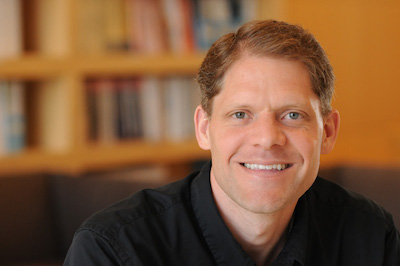
\includegraphics{img/bios/grant_jensen}

\hypertarget{mohammed_kaplan}{%
\section*{Mohammed Kaplan}\label{mohammed_kaplan}}
\addcontentsline{toc}{section}{Mohammed Kaplan}

\hypertarget{zhuo_li}{%
\section*{Zhuo Li}\label{zhuo_li}}
\addcontentsline{toc}{section}{Zhuo Li}

\hypertarget{shrawan_mageswaran}{%
\section*{Shrawan Mageswaran}\label{shrawan_mageswaran}}
\addcontentsline{toc}{section}{Shrawan Mageswaran}

\hypertarget{alasdair_mcdowall}{%
\section*{Alasdair McDowall}\label{alasdair_mcdowall}}
\addcontentsline{toc}{section}{Alasdair McDowall}

\hypertarget{lauren_ann_metskas}{%
\section*{Lauren Ann Metskas}\label{lauren_ann_metskas}}
\addcontentsline{toc}{section}{Lauren Ann Metskas}

\hypertarget{gavin_murphy}{%
\section*{Gavin Murphy}\label{gavin_murphy}}
\addcontentsline{toc}{section}{Gavin Murphy}

\hypertarget{william_nicolas}{%
\section*{William Nicolas}\label{william_nicolas}}
\addcontentsline{toc}{section}{William Nicolas}

\hypertarget{catherine_oikonomou}{%
\section*{Catherine Oikonomou}\label{catherine_oikonomou}}
\addcontentsline{toc}{section}{Catherine Oikonomou}

Catherine M. Oikonomou is a research scientist and science writer at Caltech. She received her doctorate from the Rockefeller University, where she worked with Dr.~Frederick Cross on cell cycle control in budding yeast. In 2012, she joined the lab of Dr.~Grant Jensen at Caltech, where she has been exploring microbial cell biology through cryo-electron tomography.

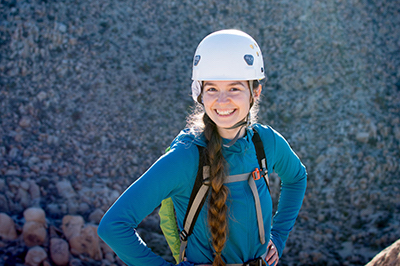
\includegraphics{img/bios/catherine_oikonomou}

\hypertarget{martin_pilhofer}{%
\section*{Martin Pilhofer}\label{martin_pilhofer}}
\addcontentsline{toc}{section}{Martin Pilhofer}

\hypertarget{sahand_pirbadian}{%
\section*{Sahand Pirbadian}\label{sahand_pirbadian}}
\addcontentsline{toc}{section}{Sahand Pirbadian}

\hypertarget{rasika_ramdasi}{%
\section*{Rasika Ramdasi}\label{rasika_ramdasi}}
\addcontentsline{toc}{section}{Rasika Ramdasi}

\hypertarget{jian_shi}{%
\section*{Jian Shi}\label{jian_shi}}
\addcontentsline{toc}{section}{Jian Shi}

\hypertarget{poorna_subramanian}{%
\section*{Poorna Subramanian}\label{poorna_subramanian}}
\addcontentsline{toc}{section}{Poorna Subramanian}

\hypertarget{matthew_swulius}{%
\section*{Matthew Swulius}\label{matthew_swulius}}
\addcontentsline{toc}{section}{Matthew Swulius}

\hypertarget{elitza_tocheva}{%
\section*{Elitza Tocheva}\label{elitza_tocheva}}
\addcontentsline{toc}{section}{Elitza Tocheva}

\hypertarget{steven_wang}{%
\section*{Steven Wang}\label{steven_wang}}
\addcontentsline{toc}{section}{Steven Wang}

\hypertarget{elizabeth_wright}{%
\section*{Elizabeth Wright}\label{elizabeth_wright}}
\addcontentsline{toc}{section}{Elizabeth Wright}

\hypertarget{qing_yao}{%
\section*{Qing Yao}\label{qing_yao}}
\addcontentsline{toc}{section}{Qing Yao}

\hypertarget{tree}{%
\chapter{Phylogenetic Tree}\label{tree}}

A species is a unique group of organisms and is the first rung on the ladder of taxonomic classifications that stretches all the way up to the three domains of life: Bacteria, Archaea and Eukarya. How \emph{exactly} a species is defined, though, is a surprisingly complicated question, especially for single-celled organisms. For most animals, species boundaries are defined by the infertility of offspring from matings across that boundary. This does not always work, though, and many species are defined by geographical, rather than reproductive, separation. For organisms that reproduce asexually, the boundaries are even more nebulous and often simply reflect a fairly arbitrary degree of difference, either morphological or genetic. Also, remember that bacteria and archaea frequently exchange genes, or larger stretches of DNA, through horizontal gene transfer (for a familiar example, think of the transfer of antibiotic resistance). This further blurs the lines between species. In an extreme view, perhaps we should think of environments less as collections of species than as pools of genes temporarily stored in a variety of containers. Still, despite its inexactness, taxonomic classification provides a useful way to trace biological traits so we can begin to answer questions like how the machines you see in this book may have evolved.

This phylogenetic tree shows the relatedness of the species in this book. The length of the branches separating two species from their last common ancestor is proportional to the amount of time that they have been evolving separately. Remember that individual species of Bacteria and Archaea can be as evolutionarily divergent from one another as they are from us. The deeper we go into the past, toward the center of the tree, the less accurate the predictions of relatedness become. The branch point between Bacteria/Archaea and Eukaryotes is particularly hazy, and a topic of lively debate. We're still discovering new species, and even higher-order clades, and the computational tools we have to detect genetic relationships are improving, so this tree, too, will continue to evolve.

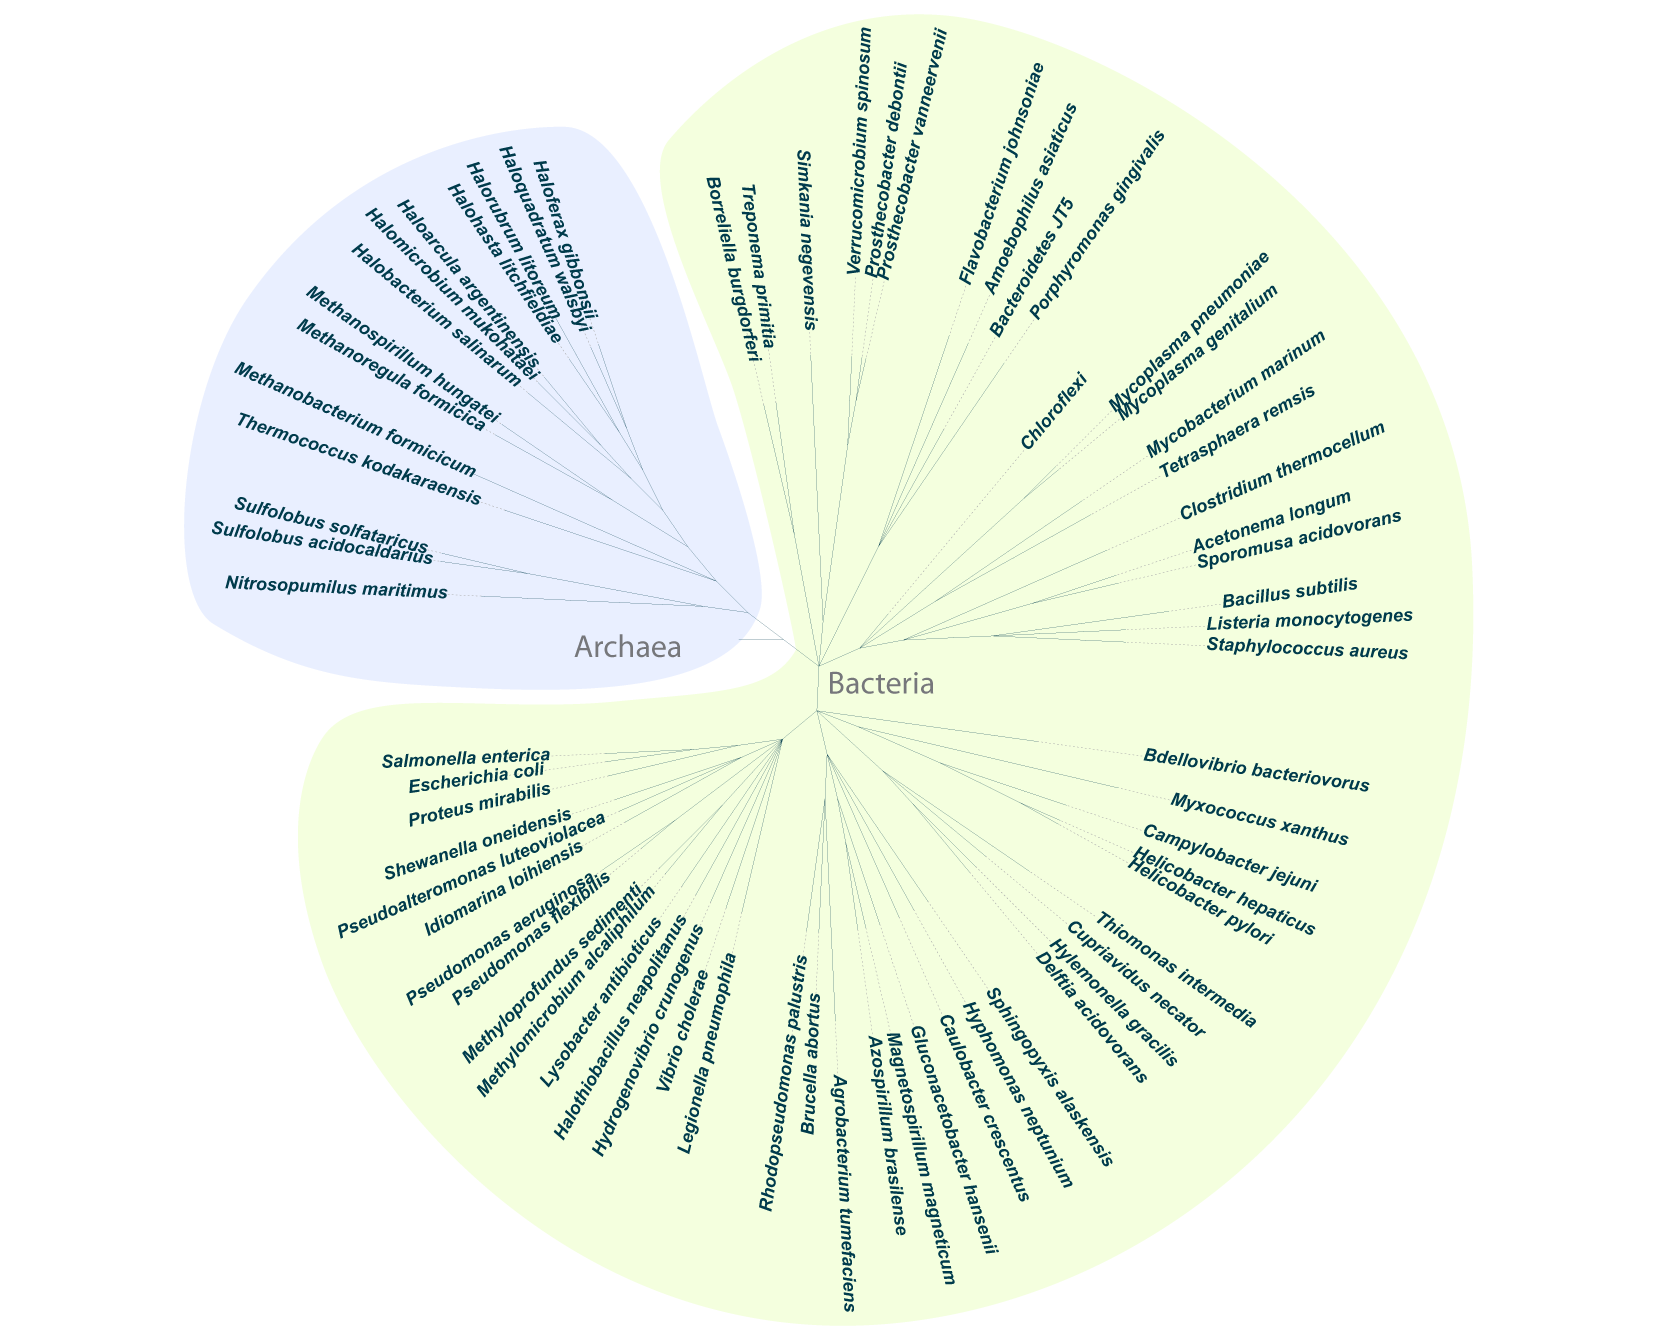
\includegraphics[width=23.06in]{img/Tree}

\hypertarget{references}{%
\chapter{References}\label{references}}

\bibliography{book.bib,packages.bib,AtlasBibTeX.bib}



\end{document}
